\chapter{Linear Algebra} \label{Sec:linearAlgebra}

The techniques of linear algebra are widely used in the field of engineering. Many practical engineering problems often involve solving partial differential equations that can rarely be solved exactly using analytical techniques of calculus. In these cases, the partial differential equations are approximated as a large system of linear equations that can be solved to obtain results that are hopefully accurate enough to make design or operational decisions. In this manner, many of the simulation tools used regularly by engineers involve the techniques of linear algebra, and it is important that engineers using those tools have a basic understanding of the underlying mathematics so as to use them appropriately.

This chapter assumes the reader has had some exposure to linear algebra. It begins by giving a quick review of the fundamental objects of linear algebra: namely matrices and vectors and their fundamental operations. 

The next topic is the change of basis, which is fundamental to understanding conversions between different coordinate systems. A key point for an engineer is that while the physics should yield the same end results, solving problems in one coordinate system versus another may prove to be significantly simpler. 

Next, linear systems of algebraic equations are covered along with a few common algorithmic techniques used to solve them. These fall into two categories: direct methods and iterative methods. The former will yield the solution (should such a unique solution exist), but is often prohibitive for the large systems of equations encountered in routine engineering calculations. The special case of the direct solve for the tridiagonal matrix is also shown, which occurs commonly in approximate solutions of differential equations. The iterative solution methods, which under certain conditions that are discussed, provide successively more accurate estimates of the solution.

Finally, the chapter reviews eigenvalues and eigenvectors. First, this concept is fundamental to understanding a key quantity in nuclear engineering: the effective multiplication factor of a system containing fissionable material, which is an eigenvalue. Furthermore, eigenvalues and eigenvectors are incredibly useful for solving linear systems of ordinary differential equations, which is discussed in the following chapter.


%%%%%%%%%%%%%%%%%%%%%%%%%%%%%%%%%%%%%%%%%%%%%%%%%%%%%%%%%%%%%%%%%%%%%%%%%%%%%%%%%%%%%%%%%%%%%%%
%%%%%%%%%%%%%%%%%%%%%%%%%%%%%%%%%%%%%%%%%%%%%%%%%%%%%%%%%%%%%%%%%%%%%%%%%%%%%%%%%%%%%%%%%%%%%%%
\section{Matrices}

A matrix is an two-dimensional object containing information. A matrix has dimensions $N$$\times$$M$, where $N$ is the number of rows and $M$ is the number of columns. A matrix can be represented as
\begin{align}
  \mathbf{A}_{N \times M} = \mathbf{A} =
  \left[ \begin{array}{c c c c} a_{1,1} & a_{1,2} & \cdots & a_{1,M} \\
  								a_{2,1} & a_{2,2} & \cdots & a_{2,M} \\
								\vdots  & \vdots  & \ddots & \vdots  \\
								a_{N,1} & a_{N,2} & \cdots & a_{N,M} \\ \end{array} \right].
\end{align}
The size subscript is given here for emphasis, but is almost always excluded.

%Certain matrices have a specific structure and are considered ``special'' because they satisfy certain properties. A list of some of these ``special'' matrices are:
%\begin{enumerate}
%  \item Square. A matrix is square if it has an equal number of rows and columns, i.e., an $N$$\times$$N$ matrix. Square matrices have special properties related to matrix multiplication and many other special matrices are square.
%  \item Symmetric. A matrix is symmetric if square and $a_{i,j} = a_{j,i}$ for all $j$ and $i$.
%  \item Diagonal. A diagonal matrix has $a_{i,j}
%\end{enumerate}

%%%%%%%%%%%%%%%%%%%%%%%%%%%%%%%%%%%%%%%%%%%%%%%%%%%%%%%%%%%%%%%%%%%%%%%%%%%%%%%%%%%%%%%%%%%%%%%
\subsection{Matrix Transpose}

The transpose operator takes a $N$$\times$$M$ matrix and constructs a $M$$\times$$N$ matrix by flipping the indices of the elements. The transpose is defined as:
\begin{align}
  \mathbf{A}^\top &= 
    \left[ \begin{array}{c c c c} a_{1,1} & a_{1,2} & \cdots & a_{1,M} \\
  		  	 					  a_{2,1} & a_{2,2} & \cdots & a_{2,M} \\
								  \vdots  & \vdots  & \ddots & \vdots  \\
								  a_{N,1} & a_{N,2} & \cdots & a_{N,M} \\ \end{array} \right]^\top 
 = \left[ \begin{array}{c c c c}  a_{1,1} & a_{2,1} & \cdots & a_{M,1} \\
  		  	 					  a_{1,2} & a_{2,2} & \cdots & a_{M,2} \\
								  \vdots  & \vdots  & \ddots & \vdots  \\
								  a_{1,N} & a_{2,N} & \cdots & a_{M,N} \\ \end{array} \right].		
\end{align}
Note that $\top$ superscript. In other words, the elements of $\mathbf{A}^\top$ are $a_{j,i}$.

The transpose satisfies several properties related to matrix addition, multiplication, and inverses that is discussed in the subsequent sections. An important property is that the transpose operation applied twice produces the original matrix:
\begin{align}
  \left( \mathbf{A}^\top \right)^\top = \mathbf{A}.
\end{align}

The transpose is mostly used when the elements are strictly real. In fields such as quantum mechanics, complex numbers of the form $a + bi$ where $i = \sqrt{-1}$, the imaginary unit, are regularly encountered. In cases where the matrix elements are complex, it is common to take the \emph{conjugate transpose} instead of just the transpose. The conjugate transpose is exactly like the transpose, in that it saws the rows and columns, but also takes the complex conjugate of each element in the resulting matrix $a + bi \rightarrow a - bi$. The conjugate transpose is denoted by a star superscript or $\mathbf{A}^*$. 

For example, consider the following matrix
\begin{align}
  \mathbf{A}  = \left[ \begin{array}{c c c} 1 & 2 + i & 0 \\ 4 & -3i & i \\ \end{array} \right] . \nonumber
\end{align}
Its conjugate transpose is
\begin{align}
  \mathbf{A}^*  = \left[ \begin{array}{c c} 1 & 4 \\ 2 - i & 3i \\ 0 & -i \end{array} \right] . \nonumber
\end{align}


%%%%%%%%%%%%%%%%%%%%%%%%%%%%%%%%%%%%%%%%%%%%%%%%%%%%%%%%%%%%%%%%%%%%%%%%%%%%%%%%%%%%%%%%%%%%%%%
\subsection{Special Types of Matrices}

Some matrices have particular forms that occur regularly in scientific and engineering applications. Furthermore, when a matrix has a particular form, it often has useful properties. In this section, a few important classes of matrices are defined. (There are numerous others that are not mentioned here.)

A matrix is said to be a \emph{square matrix} if the number of its rows and columns are equal, $N = M$. An example of a square matrix is
\begin{align}
  \mathbf{A} = 
  \left[ \begin{array}{c c c} 1 & 2 & 3 \\ 4 & 5 & 6 \\ 7 & 8 & 9 \end{array} \right]. \nonumber
\end{align}
Specifically, this is a 3$\times$3 matrix.

A matrix is said to be a \emph{diagonal matrix} if it is both a square matrix and all $a_{ij} = 0, i \ne j$. In other words, all the off-diagonal elements are zero. Three examples of diagonal matrices are
\begin{align}
  \mathbf{D} = 
  \left[ \begin{array}{c c c c} 1 & 0 & 0 & 0 \\ 0 & 2 & 0 & 0 \\ 0 & 0 & 3 & 0 \\ 0 & 0 & 0 & 4 \end{array} \right], \quad \nonumber
  \mathbf{I} = 
  \left[ \begin{array}{c c c} 1 & 0 & 0 \\ 0 & 1 & 0 \\ 0 & 0 & 1 \end{array} \right], \quad \nonumber
  \mathbf{0} = 
  \left[ \begin{array}{c c} 0 & 0  \\ 0 & 0 \end{array} \right]. \nonumber
\end{align}
The first of these is a 4$\times$4 diagonal matrix. The second example is a 3$\times$3 diagonal matrix where all elements on the diagonal are one. This is called an \emph{identity matrix}, which has special properties for matrix multiplication. The third example is a 2$\times$2 matrix where all the elements are zero. In addition to being a diagonal matrix, this is also a \emph{zero matrix}, which has special properties for matrix addition and multiplication. Note that identity matrices are always diagonal matrices whereas zero matrices can be of any size, where the latter is when all elements $a_{ij} = 0$.

A matrix is said to be a \emph{symmetric matrix} when $A = A^\top$ or $a_{ij} = a_{ji}, i \ne j$. This requires the matrix to also be a square matrix. Note that diagonal matrices are always symmetric matrices. An example of a symmetric matrix is
\begin{align}
  \mathbf{S} = 
  \left[ \begin{array}{c c c} 1 & 2 & 3 \\ 2 & 5 & 6 \\ 3 & 6 & 9 \end{array} \right]. \nonumber
\end{align}

For the case when the matrix elements are complex, we can define a \emph{Hermitian matrix} as one that is equal to its own conjugate transpose. For example, the following matrix is Hermitian:
\begin{align}
    \mathbf{H} = 
  \left[ \begin{array}{c c c} 1 & 2i & 3 - i \\ -2i & 2 & -1 \\ 3 + i & -1 & 3 \end{array} \right]. \nonumber
\end{align}
Note that a real, symmetric matrix is also Hermitian since the complex conjugate of a real number is itself.

%%%%%%%%%%%%%%%%%%%%%%%%%%%%%%%%%%%%%%%%%%%%%%%%%%%%%%%%%%%%%%%%%%%%%%%%%%%%%%%%%%%%%%%%%%%%%%%
\subsection{Column and Row Vectors}

Two special cases of matrices that are particularly important are called column and row vectors. A column vector is a matrix with a single column and $N$ rows, i.e., a $N$$\times$1 matrix and can be represented as
\begin{align}
  \mathbf{a} = 
  \left[ \begin{array}{c} a_{1} \\
  						  a_{2} \\
						  \vdots \\
						  a_{N} \end{array} \right].
\end{align}
Conversely, a row vector is a 1$\times$$N$ matrix, which may be represented as
\begin{align}
  \mathbf{a}^\top = 
  \left[ \begin{array}{c c c c} a_{1} & a_{2} & \cdots & a_{N} \end{array} \right].
\end{align}
Note the $\top$ superscript on the vector, which is the transpose operator discussed previously. The column vector is sometimes referred to as a (ordinary) vector and a row vector is sometimes called a co-vector. Both of these have geometrical interpretations that will be discussed.


%%%%%%%%%%%%%%%%%%%%%%%%%%%%%%%%%%%%%%%%%%%%%%%%%%%%%%%%%%%%%%%%%%%%%%%%%%%%%%%%%%%%%%%%%%%%%%%
\subsection{Matrix Addition, Subtraction, and Scaling}

We can add two matrices of the same dimension. If $\mathbf{A}$ and $\mathbf{B}$ are both $N$$\times$$M$, then
\begin{align}
  \mathbf{A} + \mathbf{B} &= 
    \left[ \begin{array}{c c c c} a_{1,1} & a_{1,2} & \cdots & a_{1,M} \\
  		  						  a_{2,1} & a_{2,2} & \cdots & a_{2,M} \\
		  						  \vdots  & \vdots  & \ddots & \vdots  \\
								  a_{N,1} & a_{N,2} & \cdots & a_{N,M} \\ \end{array} \right]
  +	\left[ \begin{array}{c c c c} b_{1,1} & b_{1,2} & \cdots & b_{1,M} \\
  		  						  b_{2,1} & b_{2,2} & \cdots & b_{2,M} \\
		  						  \vdots  & \vdots  & \ddots & \vdots  \\
								  b_{N,1} & b_{N,2} & \cdots & b_{N,M} \\ \end{array} \right] \nonumber	\\		
  &= \left[ \begin{array}{c c c c} a_{1,1} + b_{1,1} & a_{1,2} + b_{1,2} & \cdots & a_{1,M} + b_{1,M} \\
  		  						   a_{2,1} + b_{2,1} & a_{2,2} + b_{2,2} & \cdots & a_{2,M} + b_{2,M} \\
		  						   \vdots  & \vdots  & \ddots & \vdots  \\
								   a_{N,1} + b_{N,1} & a_{N,2} + b_{N,2} & \cdots & a_{N,M} + b_{N,M} \\ \end{array} \right] .
\end{align}
Matrix subtraction follows similarly:
\begin{align}
  \mathbf{A} - \mathbf{B} &= 
    \left[ \begin{array}{c c c c} a_{1,1} & a_{1,2} & \cdots & a_{1,M} \\
  		  						  a_{2,1} & a_{2,2} & \cdots & a_{2,M} \\
		  						  \vdots  & \vdots  & \ddots & \vdots  \\
								  a_{N,1} & a_{N,2} & \cdots & a_{N,M} \\ \end{array} \right]
  -	\left[ \begin{array}{c c c c} b_{1,1} & b_{1,2} & \cdots & b_{1,M} \\
  		  						  b_{2,1} & b_{2,2} & \cdots & b_{2,M} \\
		  						  \vdots  & \vdots  & \ddots & \vdots  \\
								  b_{N,1} & b_{N,2} & \cdots & b_{N,M} \\ \end{array} \right] \nonumber	\\		
  &= \left[ \begin{array}{c c c c} a_{1,1} - b_{1,1} & a_{1,2} - b_{1,2} & \cdots & a_{1,M} - b_{1,M} \\
  		  						   a_{2,1} - b_{2,1} & a_{2,2} - b_{2,2} & \cdots & a_{2,M} - b_{2,M} \\
		  						   \vdots  & \vdots  & \ddots & \vdots  \\
								   a_{N,1} - b_{N,1} & a_{N,2} - b_{N,2} & \cdots & a_{N,M} - b_{N,M} \\ \end{array} \right] .
\end{align}
If the two matrices being added are not the same size, then neither addition nor subtraction are defined.

Matrix addition is commutative:
\begin{align}
  \mathbf{A} + \mathbf{B} = \mathbf{B} + \mathbf{A}.
\end{align}
By extension, it is also associative:
\begin{align}
  \mathbf{A} + ( \mathbf{B} + \mathbf{C} ) = ( \mathbf{A} + \mathbf{B} ) + \mathbf{C} .
\end{align}
In other words, the order that matrices are added does not matter.

It is always possible to add the zero matrix of the appropriate size to a matrix and get the same result
\begin{align}
  \mathbf{A} + \mathbf{0} = \mathbf{A} .
\end{align}
This property is useful because many mathematical derivations involve adding $\mathbf{A} - \mathbf{A}$ to a side of an equation, which then allows for some simplification to occur.

The product of a number and a matrix simply scales all of the elements of the matrix:
\begin{align}
  r \mathbf{A} &= 
    r \left[ \begin{array}{c c c c} a_{1,1} & a_{1,2} & \cdots & a_{1,M} \\
  		  						  a_{2,1} & a_{2,2} & \cdots & a_{2,M} \\
		  						  \vdots  & \vdots  & \ddots & \vdots  \\
								  a_{N,1} & a_{N,2} & \cdots & a_{N,M} \\ \end{array} \right] \nonumber \\	
  &= \left[ \begin{array}{c c c c} r a_{1,1} & r a_{1,2} & \cdots & r a_{1,M} \\
  		  						   r a_{2,1} & r a_{2,2} & \cdots & r a_{2,M} \\
		  						   \vdots  & \vdots  & \ddots & \vdots  \\
								   r a_{N,1} & r a_{N,2} & \cdots & r a_{N,M} \\ \end{array} \right] .
\end{align}
Scalar multiplication and addition can be combined to show that matrices satisfy the distributive property:
\begin{align}
  r ( \mathbf{A} + \mathbf{B} ) = r \mathbf{A} + r \mathbf{B}.
\end{align}
In other words, we are free to add and scale or scale and then add. Note that matrix subtraction is simply a compact way of stating addition of a matrix by another matrix that has been scaled by a factor of $-1$.

If the scalar $0$ is multiplied by any matrix, the result will be the zero matrix of the same size:
\begin{align}
  0 \mathbf{A} = \mathbf{0} .
\end{align}

The matrix transpose is distributive under addition and scaling:
\begin{subequations}
\begin{align}
  &( \mathbf{A} + \mathbf{B} )^\top = \mathbf{A}^\top + \mathbf{B}^\top , \\
  &( r \mathbf{A} )^\top = r \mathbf{A}^\top.
\end{align}
\end{subequations}

%INSERT EXAMPLE HERE

%%%%%%%%%%%%%%%%%%%%%%%%%%%%%%%%%%%%%%%%%%%%%%%%%%%%%%%%%%%%%%%%%%%%%%%%%%%%%%%%%%%%%%%%%%%%%%%
\subsection{Matrix Multiplication}

The multiplication between two matrices is not as straightforward as the rules for addition, subtraction, and scaling. Suppose we have two matrices $\mathbf{A}$, which has dimension $N$$\times$$M$, and $\mathbf{B}$, which has dimension $L$$\times$$K$. We can only take the product of $\mathbf{AB}$ (note the order!) if number of columns $M$ of matrix $\mathbf{A}$ is equal to the number of rows $L$ of matrix $\mathbf{B}$, i.e., $M = L$. The result of the matrix multiplication produces an $N$$\times$$K$ matrix. If this is not the case, then matrix multiplication is not defined.

The rule for matrix multiplication is
\begin{align}
  \mathbf{C} = \mathbf{AB} &=
  \left[ \begin{array}{c c c c} a_{1,1} & a_{1,2} & \cdots & a_{1,M} \\
  								a_{2,1} & a_{2,2} & \cdots & a_{2,M} \\
								\vdots  & \vdots  & \ddots & \vdots  \\
								a_{N,1} & a_{N,2} & \cdots & a_{N,M} \\ \end{array} \right]
  \left[ \begin{array}{c c c c} b_{1,1} & b_{1,2} & \cdots & b_{1,K} \\
  								b_{2,1} & b_{2,2} & \cdots & b_{2,K} \\
								\vdots  & \vdots  & \ddots & \vdots  \\
								b_{M,1} & b_{M,2} & \cdots & b_{M,K} \\ \end{array} \right] \nonumber \\
  &= \left[ \begin{array}{c c c c} c_{1,1} & a_{1,2} & \cdots & a_{1,K} \\
  								   c_{2,1} & a_{2,2} & \cdots & a_{2,K} \\
								  \vdots  & \vdots  & \ddots & \vdots  \\
								   c_{N,1} & a_{N,2} & \cdots & a_{N,K} \\ \end{array} \right] , \nonumber \\
  &\hspace{-1cm} c_{i,j} = \sum_{k=1}^M a_{i,k} b_{k,j}.
\end{align}

Unlike multiplication between numbers, the order that the matrices are multiplied matters. In many cases, the matrix multiplication will not be defined. 

In the common case where the matrices are square (number of rows equals the number of columns) both $\mathbf{AB}$ and $\mathbf{BA}$ are defined, but {\bf not} the same. In other words, matrix multiplication is \emph{non-commutative} except for certain special cases:
\begin{align}
  \mathbf{AB} \ne \mathbf{BA}.
\end{align}
For this reason, it is important to state whether the multiplication occurs on the left or on the right. In this case matrix $\mathbf{A}$ left multiplies $\mathbf{B}$ and $\mathbf{B}$ right multiplies $\mathbf{A}$.

Matrix multiplication is associative. Suppose the product $\mathbf{ABC}$ is defined. The same result will be produced by either taking the product of $\mathbf{A}$ and $\mathbf{B}$ first and then left multiplying the result on $\mathbf{C}$ or taking the product of $\mathbf{B}$ and $\mathbf{C}$ first and then right multiplying the result on $\mathbf{A}$. In other words,
\begin{align}
  ( \mathbf{AB} ) \mathbf{C} = \mathbf{A} ( \mathbf{BC} ) .
\end{align}

Matrix multiplication is distributive so long as the multiplication is applied consistently on the left or right:
\begin{subequations}
\begin{align}
  \mathbf{A} ( \mathbf{B} + \mathbf{C} ) &= \mathbf{AB} + \mathbf{AC}, \\
  ( \mathbf{A} + \mathbf{B} ) \mathbf{C} &= \mathbf{AC} + \mathbf{BC}. 
\end{align}
\end{subequations}

Multiplication of a matrix on the left and right by the appropriately sized (square) identity matrix yields the same matrix:
\begin{align}
  \mathbf{I}_{N \times N} \mathbf{A}_{N \times M} = \mathbf{A}_{N \times M} \mathbf{I}_{M \times M} = \mathbf{A}_{N \times M}.
\end{align}
Here $\mathbf{A}$ is a N$\times$M matrix and subscripts are given to explicitly denote their size.

Likewise, multiplication of an N$\times$M matrix by an appropriately-sized zero matrix on either size yields another zero matrix:
\begin{subequations}
\begin{align}
  \mathbf{0}_{L \times N} \mathbf{A}_{N \times M} = \mathbf{0}_{L \times M}, \\
  \mathbf{A}_{N \times M} \mathbf{0}_{M \times L} = \mathbf{0}_{N \times L}.
\end{align}
\end{subequations}
Here again the subscripts are included to emphasize the sizes for didactic purposes, but are normally excluded.

Additionally, the transpose operator is distributive under matrix multiplication:
\begin{align}
  ( \mathbf{AB} )^\top = \mathbf{A}^\top \mathbf{B}^\top
\end{align}

%%%%%%%%%%%%%%%%%%%%%%%%%%%%%%%%%%%%%%%%%%%%%%%%%%%%%%%%%%%%%%%%%%%%%%%%%%%%%%%%%%%%%%%%%%%%%%%
\subsection{Linear Mapping}

Matrix multiplication has at least two geometric interpretations that are discussed in the notes. One of these is the notion of a linear map. (The other involves covectors and the discussion of that interpretation will be deferred until that section.) The notion of a linear map is important to understand coordinate transformations.

Formally, a linear map must satisfy \emph{linearity}. This implies a matrix $\mathbf{T}$ multiplied by a vectors must satisfy the following:
\begin{subequations}
\begin{align}
  &\mathbf{T}( \mathbf{x} + \mathbf{y} ) = \mathbf{Tx} + \mathbf{Ty}, \\
  &\mathbf{T}( r \mathbf{x} ) = r \mathbf{Tx}.
\end{align}
\end{subequations}
The first equation states that we may add the vectors $\mathbf{x}$ and $\mathbf{y}$ and then multiply by $\mathbf{T}$ or multiply first and then add. The second states that we may scale the vector and multiply or multiply and then scale.

To understand the linear map geometrically, let us consider the identity matrix $\mathbf{I}$ as a square $N$$\times$$N$ matrix. The columns of $\mathbf{I}$ can be thought of as unit vectors along the principal axes. In 2-D these unit vectors can be added in both orders to draw a unit square, in 3-D a unit cube, and the geometrical analogs for higher dimensions. If we then multiply $\mathbf{I}$ by $\mathbf{T}$ on the left, $\mathbf{TI} = \mathbf{T}$. The columns of the result $\mathbf{T}$ can also be interpreted and added both ways to form a parallelogram. The linear map for matrix
\begin{align}
  \mathbf{T} = 
  \left[ \begin{array}{c c}  2 &  1 \\
  							 1 & -1 \\ \end{array} \right] \nonumber
\end{align}
 maps the area within the unit square to a parallelogram described by that product. This is illustrated in Fig.~\ref{Fig:linearAlgebra_illustrationOfLinearMap} with the unprimed to the single primed basis vectors.
 
In general, suppose $\mathbf{A}$ is another square 2$\times$2 matrix that describes a parallelogram, then the multiplication $\mathbf{TA}$ maps that parallelogram to another parallelogram. In other words, all points (or differential area elements) within the parallelogram $\mathbf{A}$ are each uniquely moved to corresponding points (or differential area elements) within the parallelogram described by $\mathbf{TA}$.
 
\begin{figure}[htb!]
\begin{center}
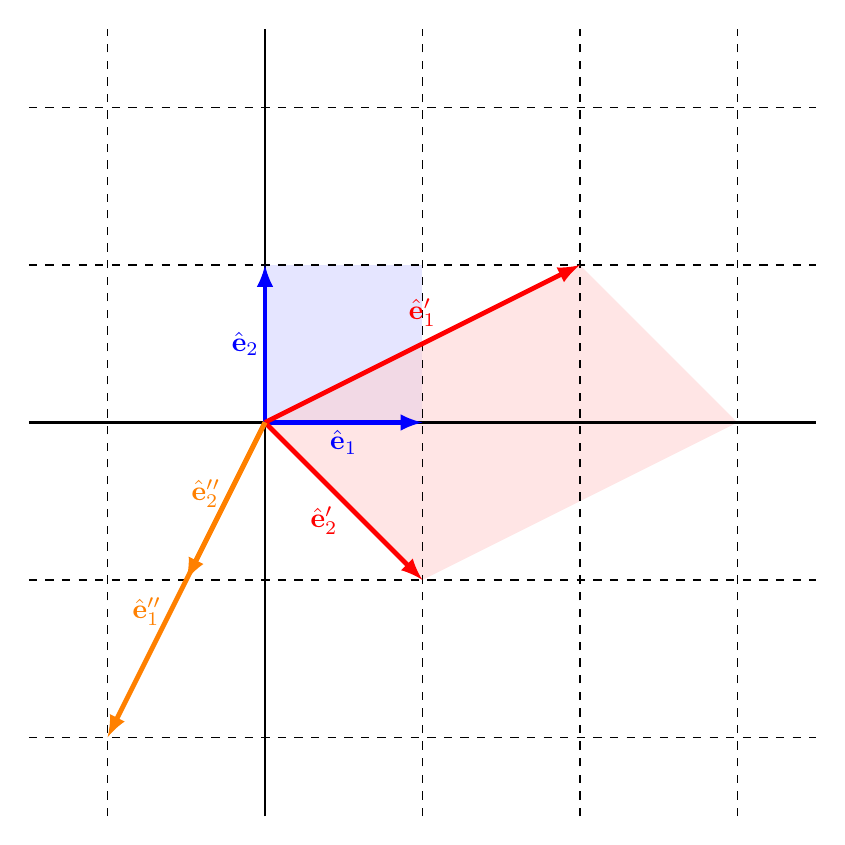
\begin{tikzpicture}
  \fill[color=blue!20,opacity=0.5] (0,0) -- (2,0) -- (2,2) -- (0,2) -- cycle;
  \fill[color=red!20,opacity=0.5]  (0,0) -- (4,2) -- (6,0) -- (2,-2) -- cycle;
  \draw[thick] (-3,0) -- (7,0);
  \draw[thick] (0,-5) -- (0,5);
  \foreach \x in {-2,0,2,4,6}
    \draw[dashed] (\x,-5) -- (\x,5);
  \foreach \y in {-4,-2,0,2,4}
    \draw[dashed] (-3,\y) -- (7,\y);
  \draw[-latex,line width=0.6mm,color=blue] (0,0) -- (2,0);
  \draw[-latex,line width=0.6mm,color=blue] (0,0) -- (0,2);
  \node[color=blue] at (1.0,-0.25) {$\hat{\mathbf{e}}_1$};
  \node[color=blue] at (-0.25,1.0) {$\hat{\mathbf{e}}_2$};
%%%  
  \draw[-latex,line width=0.6mm,color=red]  (0,0) -- (4,2);
  \draw[-latex,line width=0.6mm,color=red]  (0,0) -- (2,-2);
  \node[color=red] at (2.0,1.4)  {$\hat{\mathbf{e}}_1'$};
  \node[color=red] at (0.75,-1.25)  {$\hat{\mathbf{e}}_2'$};
%%%
  \draw[-latex,line width=0.6mm,color=orange]  (0,0) -- (-2,-4);
  \draw[-latex,line width=0.6mm,color=orange]  (0,0) -- (-1,-2);
  \node[color=orange] at (-1.5,-2.4)  {$\hat{\mathbf{e}}_1''$};
  \node[color=orange] at (-0.75,-0.9)  {$\hat{\mathbf{e}}_2''$};
\end{tikzpicture}
\caption{Illustration of a linear map of the unit square (unprimed basis vectors) to a parallelogram (single primed basis vectors) and to a line segment (double primed basis vectors).}
\label{Fig:linearAlgebra_illustrationOfLinearMap}
\end{center}
\end{figure}

This mapping can be readily extended to 3-D or any higher dimensions. In 3-D, for example, the product $\mathbf{TA}$ maps the parallelepiped described by all six combinations of sums of vectors described by the columns of $\mathbf{A}$ to another parallelepiped.

Thus far, we have looked at the case where a linear map takes an $N$ dimensional parallelotope (an $N$ dimensional analog of parallelogram) into another $N$ dimensional parallelotope. It is also possible for an $N$$\times$$N$ matrix $\mathbf{T}$ to map to a lower dimensional space. Consider the matrix,
\begin{align}
  \mathbf{T} = 
  \left[ \begin{array}{c c} -1 & -\rfrac{1}{2} \\
  							-2 & -1 \\ \end{array} \right] . \nonumber 
\end{align}
Adding the columns of $\mathbf{A}$ in both orders forms parallelogram with zero width, which is a 1-D line segment. In other words, all points (or differential area elements) in the unit square have been mapped to points (or differential line elements) on the line. This is illustrated in Fig.~\ref{Fig:linearAlgebra_illustrationOfLinearMap} with the unprimed to the double primed basis vectors.

The matrix $\mathbf{A}$ for linear maps need not be square. In these cases, the linear map will change the dimensionality of the set of vectors being operated upon.


%%%%%%%%%%%%%%%%%%%%%%%%%%%%%%%%%%%%%%%%%%%%%%%%%%%%%%%%%%%%%%%%%%%%%%%%%%%%%%%%%%%%%%%%%%%%%%%
\subsection{Matrix Determinant} \label{Sec:linearAlgebra_Matrices_MatrixDeterminant}

In this section we define an operation called the matrix determinant, which acts only on square $N$$\times$$N$ matrices denoted by
\begin{align}
  \det{A} = 
  \left| \begin{array}{c c c c} a_{1,1} & a_{1,2} & \cdots & a_{1,N} \\
  								a_{2,1} & a_{2,2} & \cdots & a_{2,N} \\
								\vdots  & \vdots  & \ddots & \vdots  \\
								a_{N,1} & a_{N,2} & \cdots & a_{N,N} \\ \end{array} \right|.
\end{align}
Note the square braces have been replaced by vertical bars.

To understand the determinant, consider the linear map discussed in the previous section, which, takes one parallelotope and transforms it into another parallelotope. In general, this linear map does not preserve the volume. (Here volume is used to mean length, area, volume, etc. depending on the dimensionality of the space) The determinant is the ratio of the volume of the transformed parallelotope to the volume of the original parallelotope, or the volume scaling factor with a sign. This sign denotes whether or not there is a flip in orientation.

The determinant of a scalar or 1$\times$1 matrix is simply the value of the scalar and just denotes that the length of the unit line is scaled by that amount.

The determinant of a 2$\times$2 matrix is the area of the parallelogram defined by the vectors in the columns of $\mathbf{A}$. The formula for the determinant is given by
\begin{align} \label{Eqn:linearAlgebra_2x2Determinant}
  \left| \begin{array}{c c} a_{1,1} & a_{1,2} \\ a_{2,1} & a_{2,2} \\ \end{array} \right| = a_{1,1} a_{2,2} - a_{1,2} a_{2,1}.
\end{align}
This formula is equivalent to the area of a parallelogram defined by the addition of the two column vectors of $\mathbf{A}$ in both orders.

A 3$\times$3 matrix can be written as the sum of three 2$\times$2 determinants:
\begin{align}
  \left| \begin{array}{c c c} a_{1,1} & a_{1,2} & a_{1,3} \\ a_{2,1} & a_{2,2} & a_{2,3} \\ a_{3,1} & a_{3,2} & a_{3,3} \\ \end{array} \right| 
  = a_{1,1} \left| \begin{array}{c c} a_{2,2} & a_{2,3} \\ a_{3,2} & a_{3,3} \\ \end{array} \right|
  - a_{1,2} \left| \begin{array}{c c} a_{2,1} & a_{2,3} \\ a_{3,1} & a_{3,3} \\ \end{array} \right|
  + a_{1,3} \left| \begin{array}{c c} a_{2,1} & a_{2,2} \\ a_{3,1} & a_{3,3} \\ \end{array} \right| .
\end{align}
Here each term includes a factor from the top row of the matrix and a 2$\times$2 determinant containing the second and third rows while excluding the column of the factor. Also note that the second term has a minus sign as opposed to a plus sign.

From these example of a 3$\times$3 determinant, we can extend the calculation of the determinant to an arbitrary number of dimensions. First, we define the quantity called the minor $M_{i,j}$ of matrix $\mathbf{A}$, which is the determinant of a submatrix $\mathbf{A}$ with the $i$th row and the $j$th column deleted. From the previous expression for a 3$\times$3 determinant, we can write, 
\begin{align}
  M_{1,1} = \left| \begin{array}{c c} a_{2,2} & a_{2,3} \\ a_{3,2} & a_{3,3} \\ \end{array} \right| , \quad
  M_{1,2} = \left| \begin{array}{c c} a_{2,1} & a_{2,3} \\ a_{3,1} & a_{3,3} \\ \end{array} \right| , \quad
  M_{1,3} = \left| \begin{array}{c c} a_{2,1} & a_{2,2} \\ a_{3,1} & a_{3,3} \\ \end{array} \right| .
\end{align}
The 2$\times$2 determinants can be evaluated using Eq.~\eqref{Eqn:linearAlgebra_2x2Determinant}. The expression for the determinant of a square matrix of size greater than 2$\times$2 is then
\begin{align}
  \det{A} = \sum_{j=1}^N (-1)^{i+j} a_{i,j} M_{i,j} ,
\end{align}
for any choice of row $i$ (usually chosen to be one). This expression is called the Laplace expansion and must be evaluated recursively, as the minors require the computation of determinants, which may themselves require computation of more determinants, reducing in size until a set of determinants of 2$\times$2 matrices can be evaluated. 

Determinants follow a few useful identities. The determinant of an N$\times$N matrix times a scaling factor $r$ is the determinant of that matrix times $r^N$,
\begin{align}
  \mathrm{det}( r \mathbf{A}_{N \times N} ) = r^N \mathrm{det}( \mathbf{A}_{N \times N} ) .
\end{align}
The determinant of a matrix is equal to the determinant of the transpose:
\begin{align}
  \mathrm{det}( \mathbf{A}^\top ) = \det{ A  } .
\end{align}
The determinant of the product of two matrices is the product of the determinants:
\begin{align}
  \det{ A B } = \det{ A } \det{ B } .
\end{align}

%The extension to higher dimensions follows in the sense that the determinant of an $N$$\times$$N$ matrix may be written as the alternating signed sum $(+-+-+\cdots)$ of $N$ determinants of $(N-1)$$\times$$(N-1)$ matrices until a sum of 2$\times$2 determinants is reached. For example, the 4$\times$4 determinant is
%\begin{align}
%  \left| \begin{array}{c c c c} a_{1,1} & a_{1,2} & a_{1,3} & a_{1,4} \\ a_{2,1} & a_{2,2} & a_{2,3} & a_{2,4} 
%                             \\ a_{3,1} & a_{3,2} & a_{3,3} & a_{3,4} \\ a_{4,1} & a_{4,2} & a_{4,3} & a_{4,4} \\ \end{array} \right| 
%  &= a_{1,1} \left| \begin{array}{c c c} a_{2,2} & a_{2,3} & a_{2,4} \\ a_{3,2} & a_{3,3} & a_{3,4} \\ a_{4,2} & a_{4,3} & a_{4,4} \\ \end{array} \right| 
%   - a_{1,2} \left| \begin{array}{c c c} a_{2,1} & a_{2,3} & a_{2,4} \\ a_{3,1} & a_{3,3} & a_{3,4} \\ a_{4,1} & a_{4,3} & a_{4,4} \\ \end{array} \right| \nonumber \\
%  &+ a_{1,3} \left| \begin{array}{c c c} a_{2,1} & a_{2,2} & a_{2,4} \\ a_{3,1} & a_{3,2} & a_{3,4} \\ a_{4,1} & a_{4,2} & a_{4,4} \\ \end{array} \right| 
%   - a_{1,4} \left| \begin{array}{c c c} a_{2,1} & a_{2,2} & a_{2,3} \\ a_{3,1} & a_{3,2} & a_{3,3} \\ a_{4,1} & a_{4,2} & a_{4,3} \\ \end{array} \right| . 
%\end{align}
%The 3$\times$3 determinants may each be expanded into three 2$\times$2 determinants, which can then be evaluated.




%The pseudocode of the recursive algorithm for computing the determinant of an $N$$\times$$N$ matrix is as follows:
%\begin{verbatim}
% function det(A)
%   if ( N == 2 )
%     return A(1,1)*A(2,2) - A(1,2)*A(2,1)
%   else
%     s = 0
%     p = 1
%     for j=1:N
%       B = new N-1 by N-1 matrix
%       m = 1
%       for i=2:N, i != j
%         for k=1
%         B(k,m) = A(k,j)
%         
%     s += p * A(1,j) * det(B)
%     p *= -1
%   return s
%\end{verbatim}

%%%%%%%%%%%%%%%%%%%%%%%%%%%%%%%%%%%%%%%%%%%%%%%%%%%%%%%%%%%%%%%%%%%%%%%%%%%%%%%%%%%%%%%%%%%%%%%
\subsection{Matrix Inverse} \label{Sec:linearAlgebra_Matrices_MatrixInverse}

If $\mathbf{A}$ is square, then we {\bf might} be able to find an inverse $\mathbf{A}^{-1}$ that satisfies the following property:
\begin{align}
  \mathbf{A}^{-1} \mathbf{A} = \mathbf{A} \mathbf{A}^{-1} = \mathbf{I}.
\end{align}
If the matrix is not square, then there is no such inverse matrix.

To show a case where the inverse does not exist, consider the matrix
\begin{align}
  \mathbf{T} = 
  \left[ \begin{array}{c c}  2 &  1 \\
  							 4 &  2 \\ \end{array} \right] . \nonumber 
\end{align}
This matrix maps the unit square onto a parallelogram of zero area, or a line segment. Now let's try to restore the unit square given by the columns of the identity matrix $\mathbf{I}$ by applying a transformation matrix $\mathbf{T}^{-1}$. For this to be true,
\begin{align}
  \mathbf{T}^{-1} \mathbf{T} &= 
     \left[ \begin{array}{c c}  a &  b \\
  							    c &  d \\ \end{array} \right]
     \left[ \begin{array}{c c}  2 &  1 \\
  				  			    4 &  2 \\ \end{array} \right] \nonumber \\
  &= \left[ \begin{array}{c c}  2a + 4b &  a + 2b \\
  				  			    2c + 4d &  c + 2d \\ \end{array} \right] 
   = \left[ \begin{array}{c c}  1 &  0 \\
  				  			    0 &  1 \\ \end{array} \right] .				   
\end{align}
The first row of the resultant matrix produces two equations:
\begin{subequations}
\begin{align}
  2a + 4b = 1, \\
   a + 2b = 0.
\end{align}
\end{subequations}
Solving the second equation yields $a = -2b$, plugging into the first gives $-4b + 4b = 0 = 1$. Since zero cannot obviously equal one, these equations are inconsistent or contradictory. It is therefore impossible to find a matrix that maps points (or differential lengths) along a line to unique points (or differential areas) within the unit square.

Recall that the resulting area of the ``parallelogram'' produced by applying matrix $\mathbf{T}$ has zero area. Therefore $\det{T} = 0$, which means the volume scaling factor is zero, and multiplication of $\mathbf{T}$ by another matrix maps any parallelogram to a line (which has zero area). By extension, it can be said that $\mathbf{T}^{-1}$ exists if and only if $\det{T} \ne 0$. Note that a matrix is said to be \emph{singular} if its inverse does not exist.

There are a few cases for which computing the inverse by solving a system of equations directly is not too difficult. The first case is the 2$\times$2 matrix. We write the equation $\mathbf{A} \mathbf{A}^{-1} = \mathbf{I}$ in the following form:
\begin{align}
  \left[ \begin{array}{c c}  a &  b \\
  							 c &  d \\ \end{array} \right]
  \left[ \begin{array}{c c}  w &  x \\
  							 y &  z \\ \end{array} \right] =
  \left[ \begin{array}{c c}  1 &  0 \\
  							 0 &  1 \\ \end{array} \right]	.						 
\end{align}
where $\left\{ a, b, c, d \right\}$ are known and $\left\{ w, x, y, z \right\}$ are unknowns. Expanding this out gives the following four equations:
\begin{subequations}
\begin{align}
  aw + by &= 1, \\
  cw + dy &= 0, \\
  ax + bz &= 0, \\
  cx + dz &= 1.
\end{align}
\end{subequations}
These are two sets of two equations with two unknowns that can be solved algebraically. Taking the first set with unknowns $w$ and $y$, we obtain,
\begin{subequations}
\begin{align}
  w &= \frac{d}{ad - bc}, \\
  y &= \frac{-c}{ad - bc},
\end{align}
and for the second set with unknowns $x$ and $z$ give,
\begin{align}
  x &= \frac{-c}{ad - bc}, \\
  z &= \frac{a}{ad - bc}.
\end{align}
\end{subequations}
Based on this result, we can write the following solution for the inverse of a 2$\times$2 matrix:
\begin{align}
  \mathbf{A}      = \left[ \begin{array}{c c} a_{1,1} & a_{1,2} \\ a_{2,1} & a_{2,2} \\ \end{array} \right], \quad
  \mathbf{A}^{-1} = \frac{1}{a_{1,1} a_{2,2} - a_{1,2} a_{2,1} } \left[ \begin{array}{c c} a_{2,2} & -a_{1,2} \\ -a_{2,1} & a_{1,1} \\ \end{array} \right] .
\end{align}
In other words, the diagonal elements are flipped, the off-diagonal elements are given a minus sign, and then the result is divided by the determinant of the original matrix. The other simple case that can be obtained directly using the direct solution approach is the inverse of a diagonal matrix:
\begin{align}
  \mathbf{D}      = \left[ \begin{array}{c c c c} d_1 & 0   & \cdots & 0 \\ 
  													0 & d_2 & \cdots & 0 \\ 
											   \vdots & \vdots & \ddots & \vdots \\
											  	    0 & 0   & \cdots & d_N \\ \end{array} \right], \quad
  \mathbf{D}^{-1} = \left[ \begin{array}{c c c c} \frac{1}{d_1} & 0   & \cdots & 0 \\ 
  													0 & \frac{1}{d_2} & \cdots & 0 \\ 
											   \vdots & \vdots & \ddots & \vdots \\
											  	    0 & 0   & \cdots & \frac{1}{d_N} \\ \end{array} \right] . \quad
\end{align}
That is, the inverse of a diagonal matrix has all of its elements being the reciprocal. 

The inverse of an arbitrary square matrix $\mathbf{A}$ can be obtained the expression:
\begin{align}
  \mathbf{A}^{-1} = \frac{1}{\det{A}} \mathbf{C}^\top,
\end{align}
provided $\det{A} \ne 0$, where $\mathbf{C}$ is called the cofactor matrix (its transpose, as in the above expression, is called the adjugate matrix). The elements of the cofactor matrix are the minors $M_{i,j}$ defined for taking the determinant (see Sec.~\ref{Sec:linearAlgebra_Matrices_MatrixDeterminant}) times a factor of $(-1)^{i+j}$. The cofactor matrix can be expressed as
\begin{align}
  \mathbf{C} = \left[ \begin{array}{c c c c c} 
      +M_{1,1} & -M_{1,2} & +M_{1,3} & \cdots & (-1)^{1+N} M_{1,N} \\ 
      -M_{2,1} & +M_{2,2} & -M_{2,3} & \cdots & (-1)^{2+N} M_{2,N} \\
      +M_{3,1} & -M_{3,2} & +M_{3,3} & \cdots & (-1)^{3+N} N_{3,N} \\
      \vdots   & \vdots   & \vdots   & \ddots & \vdots             \\
      (-1)^{N+1} M_{N,1} & (-1)^{N+2} M_{N,2} & (-1)^{N+3} M_{N,3} & \cdots &  +M_{N,N} \\ \end{array} \right] .
\end{align}
It is not too difficult to verify that the solutions for the inverses of 2$\times$2 and diagonal matrices are special cases of this result. 

While this equation provides a compact definition of the matrix inverse, it requires computation of the cofactor matrix, which involves the computation of numerous determinants. This is extremely tedious for even modestly-sized matrices and therefore this approach is not used much in practice. Rather, an algorithm computing the inverse of a matrix via a technique called Gaussian elimination is used to solve the equation $\mathbf{A} \mathbf{A}^{-1}  = \mathbf{I}$. This is discussed in Sec.~\ref{Sec:linearAlgebra_SystemsOfLinearEquations_MatrixInversion}. 

The matrix inverse has several useful properties. First, the inverse of the inverse matrix is the original matrix:
\begin{align}
  ( \mathbf{A}^{-1} )^{-1} = \mathbf{A} .
\end{align}
Also, the following scaling property is satisfied:
\begin{align}
  \left( r \mathbf{A} \right)^{-1} = \frac{1}{r} \mathbf{A}^{-1} .
\end{align}
The inverse of a product of matrices is the product of the inverse matrices in the reverse order:
\begin{align}
  ( \mathbf{AB} )^{-1} = \mathbf{B}^{-1} \mathbf{A}^{-1} .
\end{align}
The inverse of the transpose of the matrix is the transpose of the inverse matrix:
\begin{align}
  \left( \mathbf{A}^{-1} \right)^\top = \left( \mathbf{A}^\top \right)^{-1} .
\end{align}
The determinant of the inverse of a matrix is one over the determinant of the matrix:
\begin{align}
  \mathrm{det} \left( \mathbf{A}^{-1} \right) = \frac{1}{\det{A}} .
\end{align}

There is also another important special case where all the rows and columns of a square matrix are orthogonal to each other, i.e., when the sum of the products of the respective elements of all the different rows or columns of a matrix are zero (see Sec.~\ref{Sec:linearAlgebra_Vectors_Orthogonality}). If this is true, then the inverse is equal to the transpose divided by the determinant of the matrix:
\begin{align}
  \mathbf{A}^{-1} = \frac{1}{\det{A}} \mathbf{A}^\top, \quad \text{ if the rows and columns of $\mathbf{A}$ are orthogonal.}
\end{align}
A matrix is said to be an \emph{orthogonal matrix} if the inverse of the matrix is equal to its transpose, which also requires the determinant to be one in addition to what was stated above. This case arises in transformations to and from orthogonal coordinate systems. This includes all rotations as well as transformations between Cartesian, cylindrical, and spherical coordinates. (In all of these listed cases, the systems are also orthonormal, so the determinant is equal to one.) Because of this, once the transformation matrix is known in one direction, the inverse transformation in the opposite direction is simple to calculate.

In the case where the elements are complex, a matrix is said to be \emph{unitary} if the matrix times its conjugate transpose is equal to the identity matrix:
\begin{align}
  \mathbf{U} \mathbf{U}^* = \mathbf{U}^* \mathbf{U} = \mathbf{I} .
\end{align}
In other words, the conjugate transpose is its own inverse. This is a extension of the notion of an orthogonal matrix to complex elements. Note that a real orthogonal matrix is also a unitary matrix. However, a matrix with complex elements can be orthogonal but not unitary, since the transpose is not the same as the conjugate transpose. The importance of unitary matrices in quantum mechanics is that it ensures that under any transformation, the probability 


%%%%%%%%%%%%%%%%%%%%%%%%%%%%%%%%%%%%%%%%%%%%%%%%%%%%%%%%%%%%%%%%%%%%%%%%%%%%%%%%%%%%%%%%%%%%%%%
\subsection{Matrix Trace} \label{Sec:linearAlgebra_Matrices_MatrixTrace}

Another operation that sometimes arises is taking the trace of a square matrix. The trace is simply the sum of the diagonal elements:
\begin{align}
  \text{tr}( \mathbf{A} ) = \sum_{i=1}^N a_{ii} .
\end{align}
An important property is that the trace of a matrix is equal to the sum of its eigenvalues, which will be discussed later in this chapter.

%%%%%%%%%%%%%%%%%%%%%%%%%%%%%%%%%%%%%%%%%%%%%%%%%%%%%%%%%%%%%%%%%%%%%%%%%%%%%%%%%%%%%%%%%%%%%%%
%%%%%%%%%%%%%%%%%%%%%%%%%%%%%%%%%%%%%%%%%%%%%%%%%%%%%%%%%%%%%%%%%%%%%%%%%%%%%%%%%%%%%%%%%%%%%%%
\section{Vectors}

A commonly used mathematical object used to describe physical quantities such as force, momentum, electric and magnetic fields, etc. is a vector. In 3-D Cartesian coordinates, vectors are can be written in the form:
\begin{align}
  \mathbf{a} = a_x \ihat + a_y \jhat + a_z \khat.
\end{align}
This object can be represented as an arrow in three dimensional space with $a_x$ units in the $x$ direction, $a_y$ units in the $y$ direction, and $a_z$ units in the $z$ direction. Here $\ihat$, $\jhat$, and $\khat$ represent unit vectors along the respective $x$, $y$, and $z$ axes.

%Geometrically, a vector can be described by an arrow with lengths in each direction corresponding to the vector components. For example, the vector $\mathbf{a} = 2 \ihat - 3 \jhat$ can be visualized as follows: \\
%
%INSERT FIGURE HERE \\

In general 3-D coordinates, we can write a vector as
\begin{align}
  \mathbf{a} = a_1 \evec_1 + a_2 \evec_2 + a_3 \evec_3,
\end{align}
where $\evec_i$ is a vector describing the coordinate system.

In the context of matrices, the vector $\mathbf{a}$ is represented as a $N$$\times$$1$ vector or column vector. For 3-D Cartesian coordinates:
\begin{align}
  \left[ \begin{array}{c} a_x \\ a_y \\ a_z \end{array} \right] 
  = a_x \left[ \begin{array}{c} 1 \\ 0 \\ 0 \end{array} \right] 
  + a_y \left[ \begin{array}{c} 0 \\ 1 \\ 0 \end{array} \right] 
  + a_z \left[ \begin{array}{c} 0 \\ 0 \\ 1 \end{array} \right] .
\end{align}

\subsection{Addition and Scaling of Vectors}

Since vectors are a special case of a matrix, they satisfy this same addition and scaling rules. The addition (and subtraction) of two vectors is
\begin{align}
  \mathbf{a} + \mathbf{b} = ( a_x + b_x ) \ihat + ( a_y + b_y ) \jhat + ( a_z + b_z ) \khat
\end{align}
and the multiplication of a scalar $r$ and a vector is
\begin{align}
  r \mathbf{a} = r a_x \ihat + r a_y \jhat + r a_z \khat.
\end{align}


\subsection{Magnitude and Unit Vector}

A vector has a length known as is magnitude. Sometimes this is referred to as the norm, Euclidian norm, or L2-norm. The expression for computing the magnitude in \emph{Cartesian coordinates} is
\begin{align}
  | \mathbf{a} | = \sqrt{ a_x^2 + a_y^2 + a_z^2 }.
\end{align}
Here $| \cdot |$ is an operator for computing the magnitude of the vector.

A unit vector is a vector with a magnitude of one and often denoted with a hat. Given a vector $\mathbf{a}$, the corresponding unit vector may be computed as
\begin{align}
  \hat{\mathbf{a}} = \frac{ \mathbf{a} }{ | \mathbf{a} | }.
\end{align}

\subsection{Dot (Inner) Product} \label{Sec:linearAlgebra_Vectors_DotProduct}

A closely related concept to the magnitude is the \emph{dot product}, which is also called the \emph{inner product} (the dot product is a special case of the more general mathematical concept of the inner product). The dot product maps two vectors and returns a scalar. The dot product between two vectors is given as
\begin{align} \label{Eqn:linearAlgebra_DotProductDefinition}
  \mathbf{a} \cdot \mathbf{b} = | \mathbf{a} | | \mathbf{b} | \cos \theta,
\end{align}
where $\theta$ is the angle between the two vectors. Note that the definition implies commutativity of the dot product:
\begin{align}
  \mathbf{a} \cdot \mathbf{b} = \mathbf{b} \cdot \mathbf{a}.
\end{align}

To illustrate, suppose $\mathbf{a}$ and $\mathbf{b}$ are 2-D vectors in Cartesian coordinates. The dot product between them can be written as
\begin{align}
  \mathbf{a} \cdot \mathbf{b} 
  &= ( a_x \ihat + a_y \jhat ) \cdot ( b_x \ihat + b_y \jhat ) \nonumber \\
  &= a_x b_x ( \ihat \cdot \ihat ) + a_x b_y ( \ihat \cdot \jhat ) + a_y b_x ( \jhat \cdot \ihat ) + a_y b_y ( \jhat \cdot \jhat ) \nonumber \\
  &= a_x b_x ( \ihat \cdot \ihat ) + ( a_x b_y + a_y b_x ) ( \ihat \cdot \jhat ) + a_y b_y ( \jhat \cdot \jhat ) .
\end{align}
The dot products of the unit vectors can be understood through applying the right hand side of Eq.~\eqref{Eqn:linearAlgebra_DotProductDefinition}. Since $\ihat$ and $\jhat$ are unit vectors, their magnitudes are one. Furthermore, the angle between a vector and itself is $0^\circ$, which implies the dot product of the a unit vector with itself is one, i.e., $\ihat \cdot \ihat = 1, \jhat \cdot \jhat = 1$. Further, $\ihat$ and $\jhat$ are aligned along the $x$ and $y$ axes respectively, which are $90^\circ$ apart. Since $\cos 90^\circ = 0$, then $\ihat \cdot \jhat = 0$. 

By extension to 3-D (or any other number of dimensions), in Cartesian coordinates, the dot product between two vectors can be written as
\begin{align}
  \mathbf{a} \cdot \mathbf{b} = a_x b_x + a_y b_y + a_z b_z.
\end{align}
Note that this expression does {\bf not} hold in other coordinate systems, since the unit vectors may not cancel in the same way.

From a linear algebra perspective, the dot product may be written as
\begin{align}
  \mathbf{a} \cdot \mathbf{b} = \mathbf{a}^\top \mathbf{b} = 
  \left[ \begin{array}{c c c} a_x & a_y & a_z \end{array} \right] \left[ \begin{array}{c} b_x \\ b_y \\ b_z \end{array} \right] .
\end{align}
Here $\mathbf{a}^\top$ is the transpose of the vector $\mathbf{a}$.

An operation related to the dot product is finding the projection of one vector onto other. The projection of a vector $\mathbf{v}$ onto $\mathbf{u}$ is given as
\begin{align} \label{Eqn:linearAlgebra_VectorProjection}
  \text{proj}_\mathbf{u}(\mathbf{v}) = \left( \frac{ \mathbf{u} \cdot \mathbf{v} }{ \mathbf{u} \cdot \mathbf{u} } \right) \mathbf{u} .
\end{align}
The term in parentheses is a scaling factor denoting the length that $\mathbf{v}$ shadows a line through $\mathbf{u}$. The projection operator is most commonly used to generate a set of orthogonal vectors, which will be discussed later.

\subsection{Orthogonality and Orthornormality} \label{Sec:linearAlgebra_Vectors_Orthogonality}

Two different vectors are said to be orthogonal if the vectors are both of non-zero magnitude and their dot product is zero. This implies $\cos \theta = 0$, which occurs when $\theta = 90^\circ = \rfrac{\pi}{2}$ or $\theta = 270^\circ = \rfrac{3\pi}{2}$. (More generally, two different mathematical objects, e.g., functions, are orthogonal if their inner product is zero, which requires a definition of the inner product.) Given a set of orthogonal vectors $\mathbf{u}_i$, the following holds:
\begin{align}
  \mathbf{u}_i \cdot \mathbf{u}_j = c_i \delta_{ij} = \left\{ \begin{array}{c l} c_i & \quad i = j \\ 0 & \quad i \ne j \\ \end{array} \right. ,
\end{align}
with constant $c_i \ne 0$. Here $\delta_{ij}$ is called the Kronecker delta, which is one when $i = j$ and zero otherwise. The first condition for $i = j$ of this expression is a bit obvious, since the dot product of a vector with itself will always be positive (except if it is the zero vector). It is the second condition for $i \ne j$ that is not immediately apparent for an arbitrary set of vectors and is the one that should be focused on in demonstrating orthogonality and understanding the importance of this result.

Two different vectors are orthonormal if in addition to being orthogonal, they are both unit vectors (have a magnitude of one). This implies that $c_i = 1$ for all $i$ if the vectors are orthonormal.

The set of basis vectors $\mathbf{e}_i$ of the standard coordinate systems, Cartesian, cylindrical, and spherical, are orthonormal. Most work in science and engineering is in these coordinate systems, but occasionally it is more convenient to work in a coordinate system that is not. %In many applications we take a complicated domain in 2-D or 3-D and represent it approximately as a collection of triangles

The more general definition of orthogonality involving functions is useful as well and will be revisited in solutions of partial differential equations. The short version is that it is sometimes easier to solve for the integrals of the product of some orthogonal functions with the function of interest than it is to solve for that function directly.

\subsection{Cross Product} \label{Sec:linearAlgebra_Vectors_CrossProduct}

Another common application in engineering applications is the \emph{cross product}, which is denoted by $\mathbf{u} \times \mathbf{v}$. The cross product gives another vector $\mathbf{c} = \mathbf{a} \times \mathbf{b}$ that is perpendicular to $\mathbf{a}$ and $\mathbf{b}$. 

Since in 3-D space there are two vectors that are $180^\circ$ apart for each other and perpendicular to any given pair of vectors, we require a convention to pick which one. The typical convention to select this vector is the \emph{right-hand rule}. Note that this rule implies that the if we switch the order of $\mathbf{a}$ and $\mathbf{b}$, we would pick the other vector, therefore the cross product is anti-commutative, i.e.,
\begin{align}
  \mathbf{a} \times \mathbf{b} = - ( \mathbf{b} \times \mathbf{a} ).
\end{align}
Another important observation about the cross product is the it has the unusual property of being non-associative:
\begin{align}
  \mathbf{a} \times ( \mathbf{b} \times \mathbf{c} ) \ne ( \mathbf{a} \times  \mathbf{b} ) \times \mathbf{c} .
\end{align}

Computing the cross product in Cartesian coordinates involves taking the 3$\times$3 determinant. This proceeds as follows:
\begin{align}
  \mathbf{a} \times \mathbf{b} 
  &= \left| \begin{array}{c c c} \ihat & \jhat & \khat \\ a_x & a_y & a_z \\ b_x & b_y & b_z \end{array} \right|  \nonumber \\*
  &= \ihat \left| \begin{array}{c c} a_y & a_z \\ b_y & b_z \end{array} \right|
   - \jhat \left| \begin{array}{c c} a_x & a_z \\ b_x & b_z \end{array} \right|
   + \khat \left| \begin{array}{c c} a_x & a_y \\ b_x & b_y \end{array} \right| \nonumber \\*
  &= ( a_y b_z - a_z b_y ) \ihat - ( a_x b_z - a_z b_x ) \jhat + ( a_x b_y - a_z b_y ) \khat .
\end{align}
The determinant expression does not hold in non-Cartesian coordinate systems.

The cross product can also be written similarly to the dot product as
\begin{align} \label{Eqn:linearAlgebra_CrossProductDefinition}
  \mathbf{a} \times \mathbf{b} = | \mathbf{a} | | \mathbf{b} | \sin \theta \hspace{0.1cm} \nhat.
\end{align}
This expression for the cross product differs for the dot product of Eq.~\eqref{Eqn:linearAlgebra_DotProductDefinition} in two ways. First, instead of the cosine of the angle between the vector, the equation uses the sine. Secondly, the expression includes some unit vector $\nhat$, which is a unit vector perpendicular to $\mathbf{a}$ and $\mathbf{b}$.

Equation~\eqref{Eqn:linearAlgebra_CrossProductDefinition} provides a geometric interpretation of the cross product. By taking the magnitude of the cross product, $| \mathbf{a} \times \mathbf{b} |$, the right hand side becomes the area of the parallelogram formed by $\mathbf{a}$ and $\mathbf{b}$.

\subsection{Tensor (Outer) Product}

Thus far, we have studies two types of multiplication. The dot product takes two vectors and produces a scalar. The cross product takes two vectors and produces another vector perpendicular to them. There is a third type of product that produces a matrix or bivector. This is called the \emph{outer product}. The outer product of two vectors is denoted by
\begin{align}
  \mathbf{a} \otimes \mathbf{b} = \mathbf{a} \mathbf{b}^\top.
\end{align}
In the context of equations where all vectors are exclusively column vectors (common in mathematical physiscs), the product of two vectors is sometimes defined equivalently 
\begin{align}
  \mathbf{a b} \equiv \mathbf{a} \otimes \mathbf{b} .
\end{align}
This notation is called the dyadic form.

The left hand side is the product of two column vectors from linear algebra, giving a matrix. The outer product takes all combinations of component products of the two vectors and places them in the matrix. To illustrate, consider the unit vectors in 2-D space:
\begin{subequations}
\begin{align}
  \ihat \otimes \ihat &= \ihat \ihat^\top
  = \left[ \begin{array}{c} 1 \\ 0 \end{array} \right] \left[ \begin{array}{c c} 1 & 0 \end{array} \right] 
  = \left[ \begin{array}{c c} 1 & 0 \\ 0 & 0 \end{array} \right] \\
%----
  \ihat \otimes \jhat &= \ihat \jhat^\top
  = \left[ \begin{array}{c} 1 \\ 0 \end{array} \right] \left[ \begin{array}{c c} 0 & 1 \end{array} \right] 
  = \left[ \begin{array}{c c} 0 & 1 \\ 0 & 0 \end{array} \right] \\
%----
  \jhat \otimes \ihat &= \jhat \ihat^\top
  = \left[ \begin{array}{c} 0 \\ 1 \end{array} \right] \left[ \begin{array}{c c} 1 & 0 \end{array} \right] 
  = \left[ \begin{array}{c c} 0 & 0 \\ 1 & 0 \end{array} \right] \\
%----
  \jhat \otimes \jhat &= \jhat \jhat^\top
  = \left[ \begin{array}{c} 0 \\ 1 \end{array} \right] \left[ \begin{array}{c c} 0 & 1 \end{array} \right] 
  = \left[ \begin{array}{c c} 0 & 0 \\ 0 & 1 \end{array} \right] .
\end{align}
\end{subequations}
Therefore, the outer product of $\mathbf{a}$ and $\mathbf{b}$ is
\begin{align}
  \mathbf{a} \otimes \mathbf{b} 
  &= ( a_x \ihat + a_y \jhat ) \otimes ( b_x \ihat + b_y \jhat ) \nonumber \\
  &= a_x b_x ( \ihat \otimes \ihat ) + a_x b_y ( \ihat \otimes \jhat ) + a_y b_x ( \jhat \otimes \ihat ) + a_y b_y ( \jhat \otimes \jhat ) \nonumber \\
  &= a_x b_x \left[ \begin{array}{c c} 1 & 0 \\ 0 & 0 \end{array} \right] 
   + a_x b_y \left[ \begin{array}{c c} 0 & 1 \\ 0 & 0 \end{array} \right]
   + a_y b_x \left[ \begin{array}{c c} 0 & 0 \\ 1 & 0 \end{array} \right] 
   + a_y b_y \left[ \begin{array}{c c} 0 & 0 \\ 0 & 1 \end{array} \right] \nonumber \\
  &= \left[ \begin{array}{c c} a_x b_x & a_x b_y \\ a_y b_x & a_y b_y \end{array} \right] .
\end{align}
The generalization to 3-D follows the same procedure and yields a 3$\times$3 matrix.

Similar to the cross product, the outer product is not commutative. Switching the order of the outer product results in the transpose of the matrix:
\begin{align}
  \mathbf{a} \otimes \mathbf{b} = ( \mathbf{b} \otimes \mathbf{a} )^\top .
\end{align}
The outer product (unlike the cross product) is associative:
\begin{align}
  \mathbf{a} \otimes ( \mathbf{b} \otimes \mathbf{c} ) = ( \mathbf{a} \otimes \mathbf{b} ) \otimes \mathbf{c} .
\end{align}

The dot product of the a vector with the outer product of two other vectors is a vector. This arises with relative frequency in applications of fluid dynamics. The following simplification is often used based on associative rules:
\begin{align}
  \mathbf{a} \cdot ( \mathbf{b} \otimes \mathbf{c} ) = ( \mathbf{a} \cdot \mathbf{b} ) \mathbf{c} .
\end{align}
Recall the dot product is a scalar, so the overall expression is a vector.

\subsection{Scalar Triple Product}

\begin{figure}[tb!]
\begin{center}
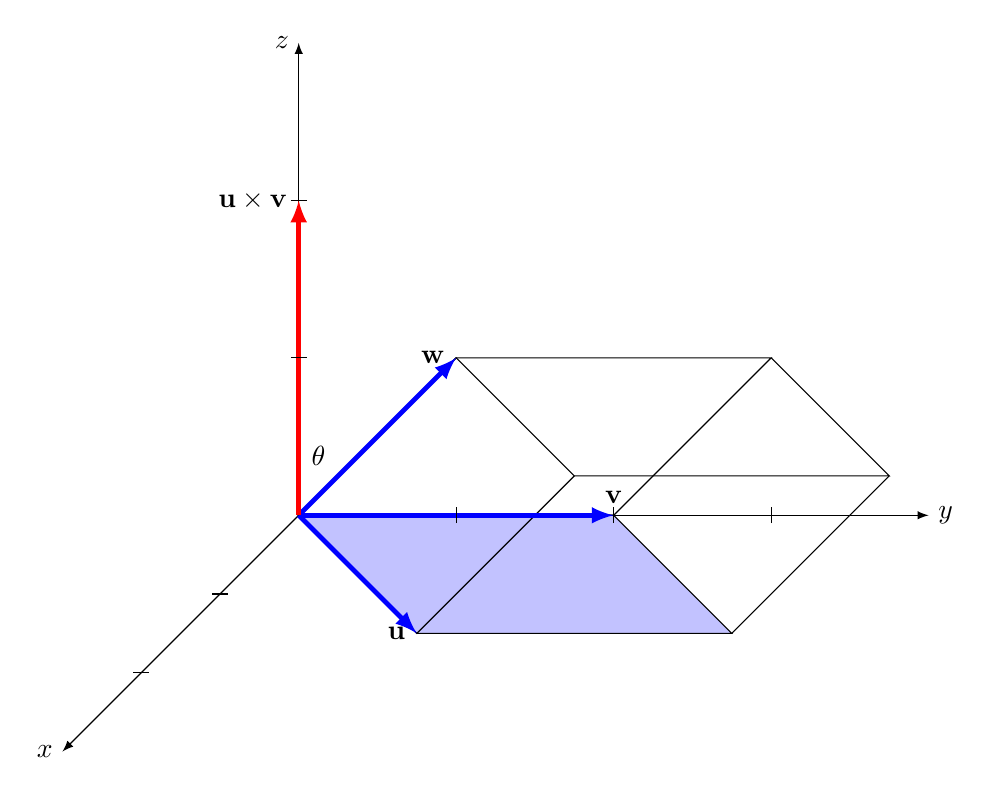
\begin{tikzpicture}[x=1cm, y=1cm, z=-0.5cm, rotate around y=0]
    % Axes
    \draw[-latex] (0,0,0) -- (8,0,0) node [right] {$y$};
    \draw[-latex] (0,0,0) -- (0,6,0) node [left] {$z$};
    \draw[-latex] (0,0,0) -- (0,0,6) node [left] {$x$};
	% Dots for atoms
%	\filldraw (0,0,0) circle (3pt);
%	\filldraw (4,0,0) circle (3pt);
%	\filldraw (0,4,0) circle (3pt);	
%	\filldraw (0,0,4) circle (3pt);	
%	\filldraw (4,4,0) circle (3pt);
% 	\filldraw (4,0,4) circle (3pt);
%	\filldraw (0,4,4) circle (3pt);
%	\filldraw (4,4,4) circle (3pt);
%	\filldraw (2,2,2) circle (3pt);
    % Vectors
    \fill[color=blue!60, opacity=0.4] (0,0,0) -- (4,0,0) -- (7,0,3) -- (3,0,3) -- cycle;

    \draw (0,0,0) -- (4,0,0) -- (7,0,3) -- (3,0,3) -- cycle;
    \draw (0,0,0) -- (2,2,0) -- (6,2,0) -- (4,0,0) -- cycle;
    \draw (0,0,0) -- (2,2,0) -- (5,2,3) -- (3,0,3) -- cycle;
    \draw (6,2,0) -- (9,2,3) -- (5,2,3);
    \draw (7,0,3) -- (9,2,3);

    \draw[-latex, line width=0.6mm,color=blue] (0,0,0) -- (3,0,3) node [left,color=black]  {$\mathbf{u}$};    
    \draw[-latex, line width=0.6mm,color=blue] (0,0,0) -- (4,0,0) node [above,color=black] {$\mathbf{v}$};
    \draw[-latex, line width=0.6mm,color=blue] (0,0,0) -- (2,2,0) node [left,color=black]  {$\mathbf{w}$};
    
    \draw[-latex, line width=0.6mm,color=red] (0,0,0) -- (0,4,0) node [left,color=black]  {$\mathbf{u} \times \mathbf{v}$};
    
    \node at (0.25,0.75,0) {$\theta$};
    
    % Ticks
        \foreach \i in {2,4}
    {
    \draw (-0.1,\i,0) -- ++ (0.2,0,0);
    \draw (\i,-0.1,0) -- ++ (0,0.2,0);
    \draw (-0.1,0,\i) -- ++ (0.2,0,0);
    }
    \draw (6,-0.1,0) -- ++ (0,0.2,0);
    % Dashed lines side atoms
%    \draw [loosely dashed]
%        (0,4,0) -- (4,4,0) -- (4,0,0)
%        (0,0,4) -- (4,0,4) -- (4,0,0)
%        (0,0,4) -- (0,4,4) -- (0,4,0)
%        (4,0,4) -- (4,4,4) -- (4,4,0)
%        (0,4,4) -- (4,4,4);
%    % Dashed lines center atom
%    \draw [loosely dashed]
%        (0,2,0) -- (2,2,0) -- (2,0,0)
%        (0,0,2) -- (2,0,2) -- (2,0,0)
%        (0,0,2) -- (0,2,2) -- (0,2,0)
%        (2,0,2) -- (2,2,2) -- (2,2,0)
%        (0,2,2) -- (2,2,2);
%%    % Labels
%     \node [right] at (2,2,0) {$\begin{bmatrix}
%                                2\\2\\0
%                               \end{bmatrix}$};
%   \node [below] at (2,0,1) {$\begin{bmatrix}
%                               2\\0\\1
%                              \end{bmatrix}$};
\end{tikzpicture}
\caption{Illustration of the scalar triple product as a computation of the volume of a parallelepided.}
\label{Fig:linearAlgebra_scalarTripleProduct_volumeParallelepided}
\end{center}
\end{figure}

The dot and cross product can be mixed to calculate the volume of a three-dimensional box with arbitrarily aligned axes called a parallelepiped. If we have three vectors defining the parallelepiped, then the signed volume can be calculated using the scalar triple product:
\begin{align}
  V = \mathbf{a} \cdot ( \mathbf{b} \times \mathbf{c} ) .
\end{align}
The sign of $V$ depends upon the orientation of the vectors, and the volume is simply the absolute value.

The interpretation of the scalar triple product as the volume is illustrated in Fig.~\ref{Fig:linearAlgebra_scalarTripleProduct_volumeParallelepided}. The vectors $\mathbf{u}$ and $\mathbf{v}$ reside in the $x$-$y$ plane and form a parallelogram (shaded in blue in the figure). The cross product between $\mathbf{u}$ and $\mathbf{v}$ (red vector) points in the $z$ direction with a magnitude corresponding to the area of this parallelogram. The vector $\mathbf{w}$ is in the $y$-$z$ plane at angle $\theta$ from the vector $\mathbf{u} \times \mathbf{v}$. Recall the dot product of these two can be expressed as is
\begin{align}
   \mathbf{w} \cdot ( \mathbf{u} \times \mathbf{v} ) = | \mathbf{u} \times \mathbf{v} | | \mathbf{w} | \cos\theta .
\end{align}
Again, the magnitude of $\mathbf{u} \times \mathbf{v}$ is the area of the base of the parallelepidped. The quantity $| \mathbf{w} | \cos\theta$ is the magnitude of the projection onto the $z$-axis (or $\mathbf{u} \times \mathbf{v}$) and is the height with respect to the base. The product of this area and height gives the volume.

In Cartesian coordinates, the scalar triple product can be computed simply by taking the determinant of a 3$\times$3 matrix where either the rows or columns correspond to the vector components. To see this we expand out the determinant for $\mathbf{b} \times \mathbf{c}$:
\begin{align}
  \mathbf{b} \times \mathbf{c} &= \left| \begin{array}{c c c} \ihat & \jhat & \khat \\ b_x & b_y & b_z \\ c_x & c_y & c_z \end{array} \right| \nonumber \\
 &= \ihat \left| \begin{array}{c c} b_y & b_z \\ c_y & c_z \end{array} \right| 
  - \jhat \left| \begin{array}{c c} b_x & b_z \\ c_x & c_z \end{array} \right|
  + \khat \left| \begin{array}{c c} b_x & b_y \\ c_x & c_y \end{array} \right| . \nonumber
\end{align}
Taking the dot product with $\mathbf{a}$ leads to the unit basis vectors being replaced the the components
\begin{align}
  \mathbf{a} \cdot ( \mathbf{b} \times \mathbf{c} ) &=
    a_x \left| \begin{array}{c c} b_y & b_z \\ c_y & c_z \end{array} \right| 
  - a_y \left| \begin{array}{c c} b_x & b_z \\ c_x & c_z \end{array} \right|
  + a_z \left| \begin{array}{c c} b_x & b_y \\ c_x & c_y \end{array} \right| . \nonumber
\end{align}
Therefore, rewriting the three minor determinants of 2$\times$2 matrices as a single 3$\times$3 determinant gives the result: 
\begin{align}
  \mathbf{a} \cdot ( \mathbf{b} \times \mathbf{c} ) = 
  \left| \begin{array}{c c c} a_x & a_y & a_z \\ b_x & b_y & b_z \\ c_x & c_y & c_z \end{array} \right| .
\end{align}
Again, it is important to note that the above expression is only valid in Cartesian coordinates.

It is not difficult to show from the determinant form, that the scalar triple product can be reordered using a circular shift, such that
\begin{align}
  \mathbf{a} \cdot ( \mathbf{b} \times \mathbf{c} ) = \mathbf{c} \cdot ( \mathbf{a} \times \mathbf{b} ) = \mathbf{b} \cdot ( \mathbf{c} \times \mathbf{a} ) .
\end{align}
A circular shift is pushing each vector forward one position in the expression and moving the entry on the end to the beginning. The cross product of any of these can be reordered with a minus sign given the anticommutativity of the cross product.

\subsection{Vector Triple Product}

Given the scalar triple product defined with the dot product of a cross product, it may be instructive to consider taking the cross product of another cross product. (Taking the cross product of a dot product does not make sense, or a dot product of a dot product does not make sense either if considering vectors.) This arises in physics when, for example, calculating centrifugal forces in a rotating coordinate system and occurs frequently in electrodynamics. The vector triple product produces another vector and is
\begin{align}
  \mathbf{v} = \mathbf{a} \times ( \mathbf{b} \times \mathbf{c} ) .
\end{align}
The computation of this can be a bit unwieldy to work out, but there is a very important vector identity to recast this vector product in terms of much simpler dot products. This identity is referred to as the ``BAC-CAB rule'', which is a useful nemonic:
\begin{align}
  \mathbf{a} \times ( \mathbf{b} \times \mathbf{c} ) = \mathbf{b} \left( \mathbf{a} \cdot \mathbf{c} \right)  - \mathbf{c} \left( \mathbf{a} \cdot \mathbf{b} \right) .
\end{align}
Note the ordering has the vector out front of the scalar in the nemonic. This identity is frequently used to simplify complex vector equations and makes the numerical computation much simpler. Unlike the scalar triple product, which has a geometric interpretation of computing a volume, there is not an analogous physical interpretation.

%%%%%%%%%%%%%%%%%%%%%%%%%%%%%%%%%%%%%%%%%%%%%%%%%%%%%%%%%%%%%%%%%%%%%%%%%%%%%%%%%%%%%%%%%%%%%%%
%%%%%%%%%%%%%%%%%%%%%%%%%%%%%%%%%%%%%%%%%%%%%%%%%%%%%%%%%%%%%%%%%%%%%%%%%%%%%%%%%%%%%%%%%%%%%%%
\section{Covectors}

If ordinary vectors are matrix equivalents of column vectors, it may be natural to ask if there is an interpretation of row vectors. Indeed there is, and this is called a covector. (In many contexts this is referred to as a linear form or an algebraic 1-form.)

To illustrate the concept, let us consider the 2-D row vector
\begin{align}
  \boldsymbol\alpha = \left[ \begin{array}{c c} 1 & \rfrac{-1}{2} \\ \end{array} \right] . \nonumber
\end{align}
Let this row vector act upon a column vector as follows to yield an equation
\begin{align}
  \left[ \begin{array}{c c} 1 & \rfrac{-1}{2} \\ \end{array} \right] 
  \left[ \begin{array}{c} x \\ y \\ \end{array} \right] = x - \frac{y}{2} = r, \nonumber
\end{align}
here $r$ is some scalar value that is the numerical result for a given values of $(x,y)$. This equation denotes the equation for the line $y = 2x - 2r$. If we plot a series of lines for various values of $r$, we have the geometric representation of the covector (see Fig.~\ref{Fig:linearAlgebra_vectorAndCovectorIllustration}). This can be thought of as a series of contour lines with a provided orientation given by the small black arrows normal to those lines that point toward larger values of $r$. In 3-D the covector is represented graphically a stack of planes with a provided orientation. Covectors may also be represented in a similar manner in higher dimensions, but this is harder to visualize.

Similar to vectors, we can express covectors in terms of basis covectors:
\begin{align}
  \boldsymbol\alpha = \alpha_1 \boldsymbol\epsilon_1 + \alpha_2 \boldsymbol\epsilon_2 + \ldots
\end{align}
In 2-D Cartesian coordinates the basis covectors $\boldsymbol\epsilon_1, \boldsymbol\epsilon_2$ are $\mathbf{e}_1^\top = \ihat^\top$ and $\mathbf{e}_2^\top = \jhat^\top$. These represent the lines $x = r$ and $y = r$ respectively for given parameter $r$ with orientation pointing toward the positive $x$ and $y$ directions.

\begin{figure}[htb!]
\begin{center}
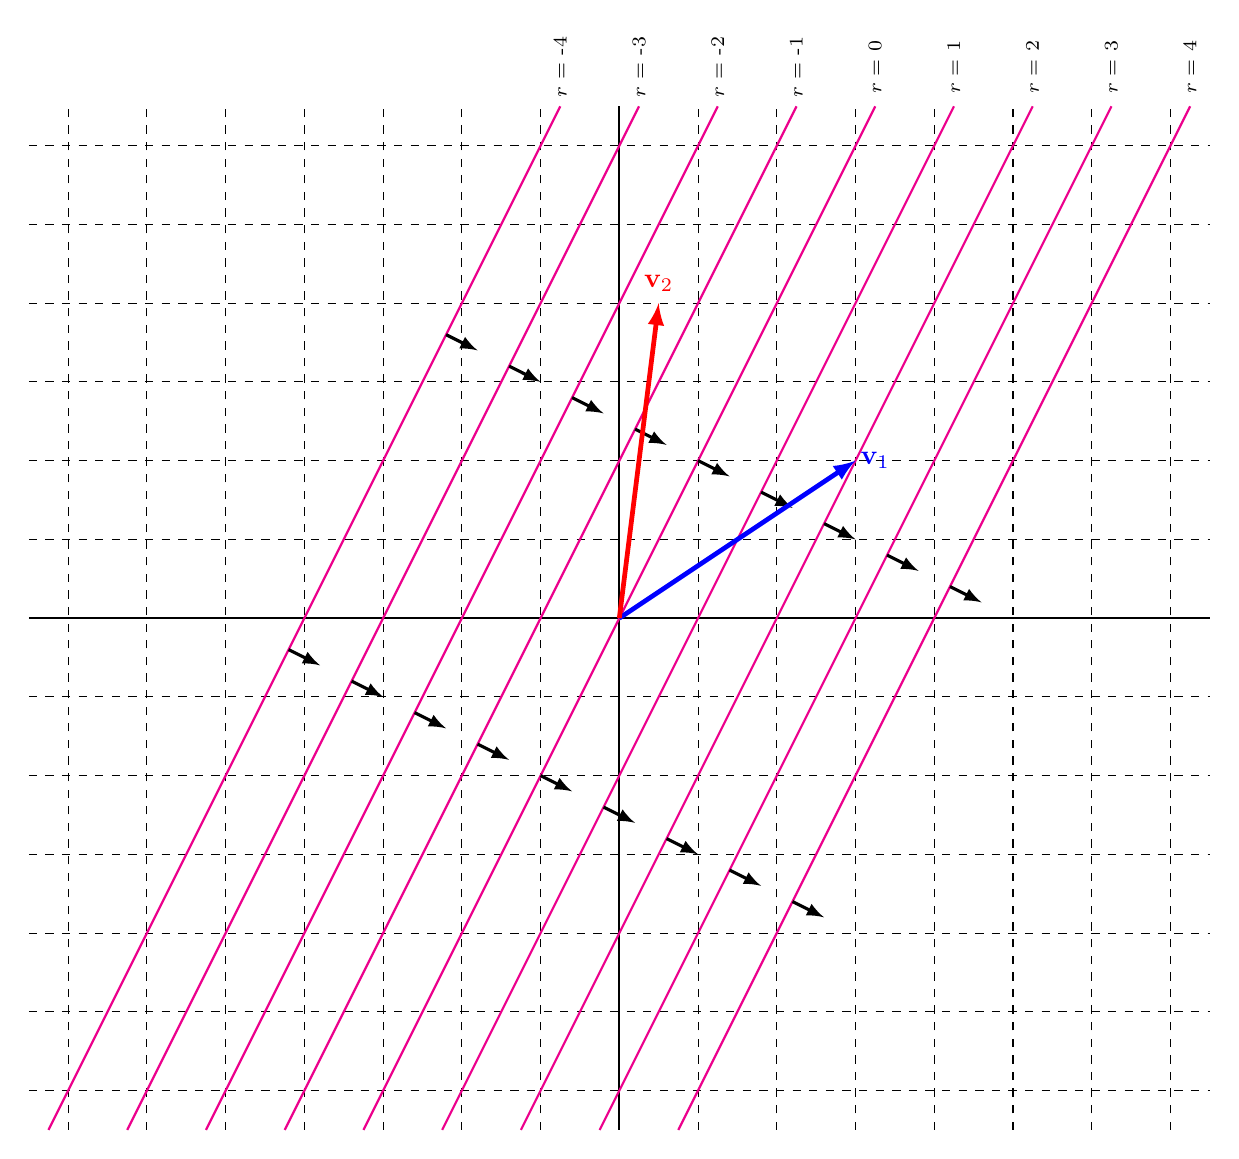
\begin{tikzpicture}
  \draw[thick] (-7.5,0) -- (7.5,0);
  \draw[thick] (0,-6.5) -- (0,6.5);
  \foreach \x in {-7,...,7}
    \draw[dashed] (\x,-6.5) -- (\x,6.5);
  \foreach \y in {-6,...,6}
    \draw[dashed] (-7.5,\y) -- (7.5,\y);
  \foreach \r in {-4,...,4} {
    \draw[thick,color=magenta] (-3.25 + \r,-6.5) -- (3.25 + \r,6.5);
    \node[rotate=90] at (3.25 + \r,7)  {\scriptsize $r = $ \r};
    \draw[-latex,line width=0.4mm] (0.8*\r + 1, -0.4*\r + 2) -- +(0.4,-0.2);
    \draw[-latex,line width=0.4mm] (0.8*\r - 1, -0.4*\r - 2) -- +(0.4,-0.2);
  }
  \draw[-latex,line width=0.6mm,color=blue] (0,0) -- (3,2);
  \draw[-latex,line width=0.6mm,color=red] (0,0) -- (0.5,4);
  \node[color=blue] at (3.25,2) {$\mathbf{v}_1$};
  \node[color=red] at (0.5,4.25) {$\mathbf{v}_2$};
\end{tikzpicture}
\caption{Illustration of vectors and a covector.}
\label{Fig:linearAlgebra_vectorAndCovectorIllustration}
\end{center}
\end{figure}

%\begin{figure}[htb!]
%\begin{center}
%\begin{tikzpicture}
%  \draw[thick] (-4.5,0) -- (4.5,0);
%  \draw[thick] (0,-4.5) -- (0,4.5);
%  \foreach \x in {-4,...,4}
%    \draw[dashed] (\x,-4.5) -- (\x,4.5);
%  \foreach \y in {-4,...,4}
%    \draw[dashed] (-4.5,\y) -- (4.5,\y);
%  \foreach \r in {-2,...,2} {
%    \draw[thick,color=magenta] (-2.25 + \r,-4.5) -- (2.25 + \r,4.5);
%    \node at (2.25 + \r,4.75)  {\scriptsize $r = $ \r};
%    \draw[-latex,line width=0.4mm] (0.8*\r + 1, -0.4*\r + 2) -- +(0.4,-0.2);
%    \draw[-latex,line width=0.4mm] (0.8*\r - 1, -0.4*\r - 2) -- +(0.4,-0.2);
%  }
%  \draw[-latex,line width=0.6mm,color=blue] (0,0) -- (3,2);
%  \draw[-latex,line width=0.6mm,color=red] (0,0) -- (0.5,4);
%  \node[color=blue] at (3.25,2) {$\mathbf{v}_1$};
%  \node[color=red] at (0.5,4.25) {$\mathbf{v}_2$};
%\end{tikzpicture}
%\caption{Illustration of vectors and a covector.}
%\label{Fig:linearAlgebra_vectorAndCovectorIllustration}
%\end{center}
%\end{figure}

%%%%%%%%%%%%%%%%%%%%%%%%%%%%%%%%%%%%%%%%%%%%%%%%%%%%%%%%%%%%%%%%%%%%%%%%%%%%%%%%%%%%%%%%%%%%%%%
\subsection{Covectors and Matrix Multiplication} \label{Sec:linearAlgebra_Covectors_CovectorsAndMatrixMultiplication}

Covector-vector multiplication gives us a second geometric interpretation of matrix multiplication (the first being a linear map).

A covector may operate on a vector to produce a number in the same manner as matrix multiplication or the dot product as follows:
\begin{align}
  \boldsymbol{\alpha}(\mathbf{v}) = \sum_i \alpha_i v_i.
\end{align}
More interesting is the geometric interpretation. Suppose now that our former 2-D covector
\begin{align}
  \boldsymbol\alpha = \left[ \begin{array}{c c} 1 & \rfrac{-1}{2} \\ \end{array} \right]  \nonumber
\end{align}
acts on a vector
\begin{align}
  \mathbf{v}_1 = \left[ \begin{array}{c} 3 \\ 2 \\ \end{array} \right] . \nonumber
\end{align}
The result of $\boldsymbol\alpha(\mathbf{v}_1)$ is 2. This is plotted graphically in Fig.~\ref{Fig:linearAlgebra_vectorAndCovectorIllustration} in blue. We could think of the lines formed by a covector as contour lines on a physical map, which describe lines of constant elevation. The covector-vector multiplication can therefore be thought of as a change in elevation or a kind of signed distance measured with respect to the covector planes. In this specific case, the ``distance'' measured is 2 because the vector travels right up to the second covector line. Also, the length is positive the directionality with respect to the covector (going in the same direction as the small black arrows). Considering another vector
\begin{align}
  \mathbf{v}_2 = \left[ \begin{array}{c} \rfrac{1}{2} \\ 4 \\ \end{array} \right] , \nonumber
\end{align}
$\boldsymbol\alpha(\mathbf{v}_2)$ is $\rfrac{-3}{2}$, which is plotted in Fig.~\ref{Fig:linearAlgebra_vectorAndCovectorIllustration} in red. This means the vector travels a ``distance'' of $\rfrac{3}{2}$ with respect to the covector---the vector crosses one line and gets halfway to the next---but in the negative direction since the vector is crossing the lines in the opposite direction of their orientation. Note that the length is negative despite both components of $\mathbf{v}_2$ being positive; the sign is with respect to the orientation of the covector.

The second geometric interpretation of matrix multiplication $\mathbf{C} = \mathbf{AB}$ is that each element in the resultant matrix $c_{i,j}$ is a signed ``distance'' of a vector defined by column $j$ of $\mathbf{B}$ measured with respect to the planes of the covector defined by row $i$ of $\mathbf{A}$. More precisely ``signed distance'' can be thought of as a change in some quantity in a field, e.g., the work done in the presence of a force field.


%%%%%%%%%%%%%%%%%%%%%%%%%%%%%%%%%%%%%%%%%%%%%%%%%%%%%%%%%%%%%%%%%%%%%%%%%%%%%%%%%%%%%%%%%%%%%%%
%%%%%%%%%%%%%%%%%%%%%%%%%%%%%%%%%%%%%%%%%%%%%%%%%%%%%%%%%%%%%%%%%%%%%%%%%%%%%%%%%%%%%%%%%%%%%%%
\section{Coordinate Systems}

Engineering calculations require making a choice of coordinate system. Most often, the Cartesian coordinate system is sufficient. Other times, we must work in other common coordinate systems such as cylindrical or spherical coordinates. Occasionally, we will need to work in other nonstandard coordinate systems as well. Coordinate systems are described by a set of vectors called basis vectors, which can be thought of as the fundamental building blocks that can be used to construct any vector in that coordinate system. Moving from one coordinate system to another is referred to as a change of basis. The notion of a basis can be extended to not just include vectors, but can also include any object such as polynomials or matrices. This section will review the concepts of linear independence, span, a basis, and then transformations for converting between different coordinate systems.

%%%%%%%%%%%%%%%%%%%%%%%%%%%%%%%%%%%%%%%%%%%%%%%%%%%%%%%%%%%%%%%%%%%%%%%%%%%%%%%%%%%%%%%%%%%%%%%
\subsection{Linear Independence}

Coordinate systems are defined by a set of linearly independent vectors called basis vectors. For this reason, we need to define the concept of linear independence. Suppose we have a set of vectors $\left\{ \mathbf{v}_1, \mathbf{v}_2, \cdots , \mathbf{v}_N \right\}$. We say that some vector in the set $\mathbf{v}_k$ for $k = 1, \ldots , N$ is linearly independent of the others if and only if $\mathbf{v}_k$ cannot be expressed as a linear combination of the others. Conversely, a vector is linearly dependent (not linearly independent) if
\begin{align}
  \mathbf{v}_k = \sum_{\substack{i = 1\\ i\ne k}}^N a_i \mathbf{v}_i ,
\end{align}
for some choice of nonzero coefficients $a_i$.

For example, consider the set of two-dimensional vectors
\begin{align}
  \mathbf{v}_1 = \left[ \begin{array}{c} 1 \\  0 \\ \end{array} \right] , \quad
  \mathbf{v}_2 = \left[ \begin{array}{c} 1 \\ -1 \\ \end{array} \right] , \quad  
  \mathbf{v}_3 = \left[ \begin{array}{c} 2 \\  1 \\ \end{array} \right] .
\end{align}
It is fairly evident that this set of vectors is linearly dependent. To show this, we can find a counterexample. We express $\mathbf{v}_3 = 3 \mathbf{v}_1 - \mathbf{v}_2$ or
\begin{align}
   3 \left[ \begin{array}{c} 1 \\  0 \\ \end{array} \right]
 -   \left[ \begin{array}{c} 1 \\ -1 \\ \end{array} \right] =
     \left[ \begin{array}{c} 3 \\  0 \\ \end{array} \right]  
 +   \left[ \begin{array}{c} -1 \\ 1 \\ \end{array} \right] =
   \left[ \begin{array}{c} 2 \\  1 \\ \end{array} \right]
\end{align}
Note that if we pick any two of the vectors from this set, those vectors are linearly independent. This is very simple to show since there is no single scalar that we can multiply by one of the vectors to get the other. 

An important observation is that if the vectors in the set are $N$ dimensional, then if there are more than $N$ vectors in the set, the set cannot be linearly independent. The converse is not true. Just because there are $N$ or fewer $N$-dimensional vectors in the set, that does not imply the vectors are linearly independent.

For another example, consider the set of vectors
\begin{align}
  \mathbf{v}_1 = \left[ \begin{array}{c} 1 \\  0 \\ 2 \\ \end{array} \right] , \quad
  \mathbf{v}_2 = \left[ \begin{array}{c} 1 \\ -1 \\ 0 \\ \end{array} \right] , \quad  
  \mathbf{v}_3 = \left[ \begin{array}{c} 0 \\  1 \\ 1 \\ \end{array} \right] .
\end{align}
We can show that $\mathbf{v}_1$ cannot be written as a linear combination of $\mathbf{v}_2$ and $\mathbf{v}_3$. Let us suppose that there exists nonzero coefficients $a_1$ and $a_2$ such that
\begin{align}
  \left[ \begin{array}{c} 1 \\  0 \\ 2 \\ \end{array} \right] \stackrel{?}{=} 
  a_1  \left[ \begin{array}{c} 1 \\ -1 \\ 0 \\ \end{array} \right] + a_2 \left[ \begin{array}{c} 0 \\  1 \\ 1 \\ \end{array} \right] . \nonumber
\end{align}
This forms the linear system of equations
\begin{align}
  a_1 = 1, \quad a_2 - a_1 = 0, \quad a_2 = 2, \nonumber
\end{align}
The first and third equations are inconsistent with the second, since $2 - 1 \ne 0$. Therefore, $\mathbf{v}_1$ is linearly independent of $\mathbf{v}_2$ and $\mathbf{v}_3$.

A test for whether a set of $N$ vectors each having a length $N$ is linearly independent is to check whether the determinant of a matrix having the columns be given by those vectors is nonzero. Using the previous example
\begin{align}
  \left| \begin{array}{c c c}  
    1 &  1 &  0 \\
    0 & -1 &  1 \\
    2 &  0 &  1 \\ \end{array} \right| = (1)(-1 - 0) - (1)(0 - 2) + (0)( -1 - 0 ) = -1 + 2 = 1 . \nonumber
\end{align}
By this test, the vectors are linearly independent.

A very similar, but non-trivial case where the vectors are linearly dependent is
\begin{align}
  \mathbf{v}_1 = \left[ \begin{array}{c} 1 \\  0 \\ 2 \\ \end{array} \right] , \quad
  \mathbf{v}_2 = \left[ \begin{array}{c} 1 \\ -1 \\ 0 \\ \end{array} \right] , \quad  
  \mathbf{v}_3 = \left[ \begin{array}{c} 0 \\  1 \\ 2 \\ \end{array} \right] . \label{Eqn:linearAlgebra_linearIndepndence_dependentVectors}
\end{align}
The only difference from the previous example is the vector $\mathbf{v}_3$. This can be simply shown by forming the linear system as before
\begin{align}
  a_1 = 1, \quad a_2 - a_1 = 0, \quad 2 a_2 = 2 . \nonumber
\end{align}
This time $a_1 = 1$ and $a_2 = 1$, so the second equation is satisfied. Therefore, the system is linearly dependent. Alternatively, we can compute the determinant
\begin{align}
  \left| \begin{array}{c c c}  
    1 &  1 &  0 \\
    0 & -1 &  1 \\
    2 &  0 &  2 \\ \end{array} \right| = (1)(-2 - 0) - (1)(0 - 2) + (0)( -1 - 0 ) = -2 + 2 = 0 . \nonumber
\end{align}

\begin{figure}[tb!]
\begin{center}
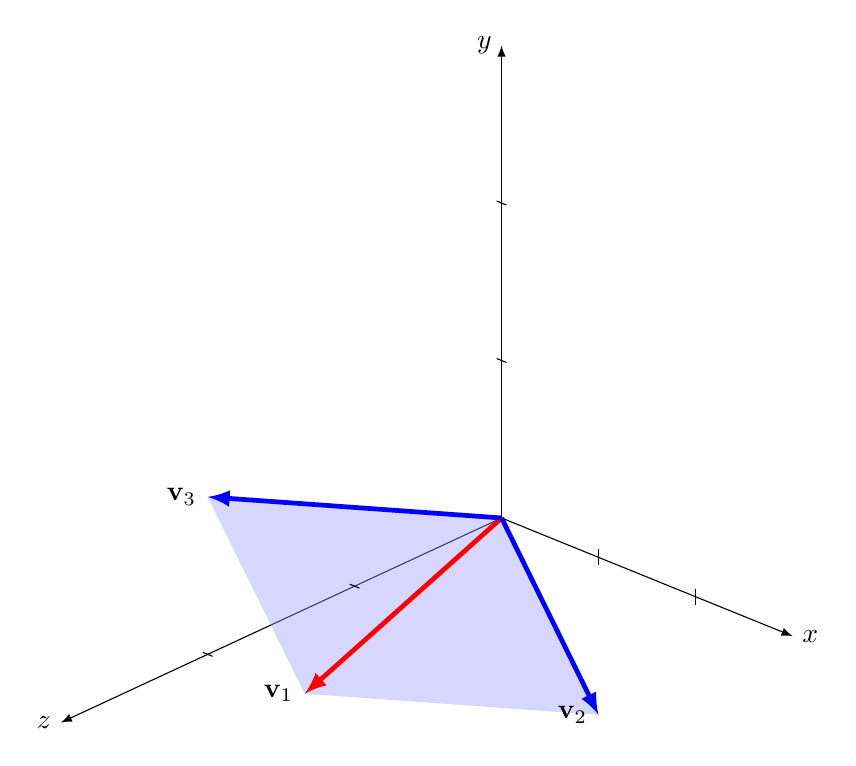
\begin{tikzpicture}[x=1cm, y=1cm, z=-0.5cm, rotate around y=-30]
    % Axes
    \draw[-latex] (0,0,0) -- (6,0,0) node [right] {$x$};
    \draw[-latex] (0,0,0) -- (0,6,0) node [left] {$y$};
    \draw[-latex] (0,0,0) -- (0,0,6) node [left] {$z$};
    % Plane
    \fill[color=blue!40, opacity=0.4] (0,0,0) -- (2,-2,0) -- (2,0,4) -- (0,2,4) -- cycle;
    % Vectors
    \draw[-latex, line width=0.6mm,color=red]  (0,0,0) -- (2, 0,4) node [left,color=black]  {$\mathbf{v}_1$};
    \draw[-latex, line width=0.6mm,color=blue] (0,0,0) -- (2,-2,0) node [left,color=black]  {$\mathbf{v}_2$};
    \draw[-latex, line width=0.6mm,color=blue] (0,0,0) -- (0, 2,4) node [left,color=black]  {$\mathbf{v}_3$};
    % Ticks
        \foreach \i in {2,4}
    {
    \draw (-0.1,\i,0) -- ++ (0.2,0,0);
    \draw (\i,-0.1,0) -- ++ (0,0.2,0);
    \draw (-0.1,0,\i) -- ++ (0.2,0,0);
    }
\end{tikzpicture}
\caption{Example of linearly dependent vectors where $\mathbf{v}_1$ is on the plane formed by $\mathbf{v}_2$ and $\mathbf{v}_3$.}
\label{Fig:linearAlgebra_linearIndepndenceGeometric_example}
\end{center}
\end{figure}

Before proceeding, let us consider the geometric interpretation by way of looking at the example where the vectors are linearly dependent. The vectors $\mathbf{v}_2$ and $\mathbf{v}_3$ can be used to form a plane in 3-D space. The vector $\mathbf{v}_1$ is within this plane. This is illustrated in Fig.~\ref{Fig:linearAlgebra_linearIndepndenceGeometric_example}. Geometrically, three vectors that are linearly independent do not exist in the same plane.

%%%%%%%%%%%%%%%%%%%%%%%%%%%%%%%%%%%%%%%%%%%%%%%%%%%%%%%%%%%%%%%%%%%%%%%%%%%%%%%%%%%%%%%%%%%%%%%%
\subsection{Basis and Span}

A basis can be thought of as the fundamental linearly independent building blocks (e.g., vectors) that can be used to construct a particular class of objects by way of a linear combination. The span is the smallest set of these vectors that can be used to create the class.

The most common example encountered in engineering applications is the set of all real numbers in 3-D space, denoted by $\mathbb{R}^3$. This can be described by the unit basis vectors $\{ \ihat, \jhat, \khat \}$. Equivalently all 3-D vectors can be defined by
\begin{align}
  \text{span} \left\{ 
    \left[ \begin{array}{c} 1 \\  0 \\ 0 \\ \end{array} \right] ,
    \left[ \begin{array}{c} 0 \\  1 \\ 0 \\ \end{array} \right] ,
    \left[ \begin{array}{c} 0 \\  0 \\ 1 \\ \end{array} \right] \right\}
  = a_1 \left[ \begin{array}{c} 1 \\  0 \\ 0 \\ \end{array} \right] 
  + a_2 \left[ \begin{array}{c} 0 \\  1 \\ 0 \\ \end{array} \right]
  + a_3 \left[ \begin{array}{c} 0 \\  0 \\ 1 \\ \end{array} \right] .
\end{align}
Note that the unit basis vectors are a convenient choice for the span of $\mathbb{R}^3$. In reality, any three linearly independent 3-dimensional vectors would suffice.

Another example is the space of all vectors that live in a plane in 3-D space. Considering the vectors from Eq.~\eqref{Eqn:linearAlgebra_linearIndepndence_dependentVectors}, we can compute the equation for the plane that intersects the origin by taking the cross product of two of the vectors with the coefficients being the components of that vector:
\begin{align}
  2x + 2y - z = 0. \nonumber
\end{align}
The span of all vectors on this plane consists of any two linearly independent vectors. For instance, the vectors $\mathbf{v}_1$ and $\mathbf{v}_2$ satisfy this criteria:
\begin{align}
  \text{span} \left\{ 
    \left[ \begin{array}{c} 1 \\  0 \\ 2 \\ \end{array} \right] ,
    \left[ \begin{array}{c} 1 \\ -1 \\ 0 \\ \end{array} \right] \right\}
  = a_1 \left[ \begin{array}{c} 1 \\  0 \\ 2 \\ \end{array} \right] 
  + a_2 \left[ \begin{array}{c} 1 \\ -1 \\ 0 \\  \end{array} \right] .
\end{align}
Any other pair of linearly independent vectors on the plane would suffice as arguments of the span.

\begin{figure}[htb!]
\begin{center}
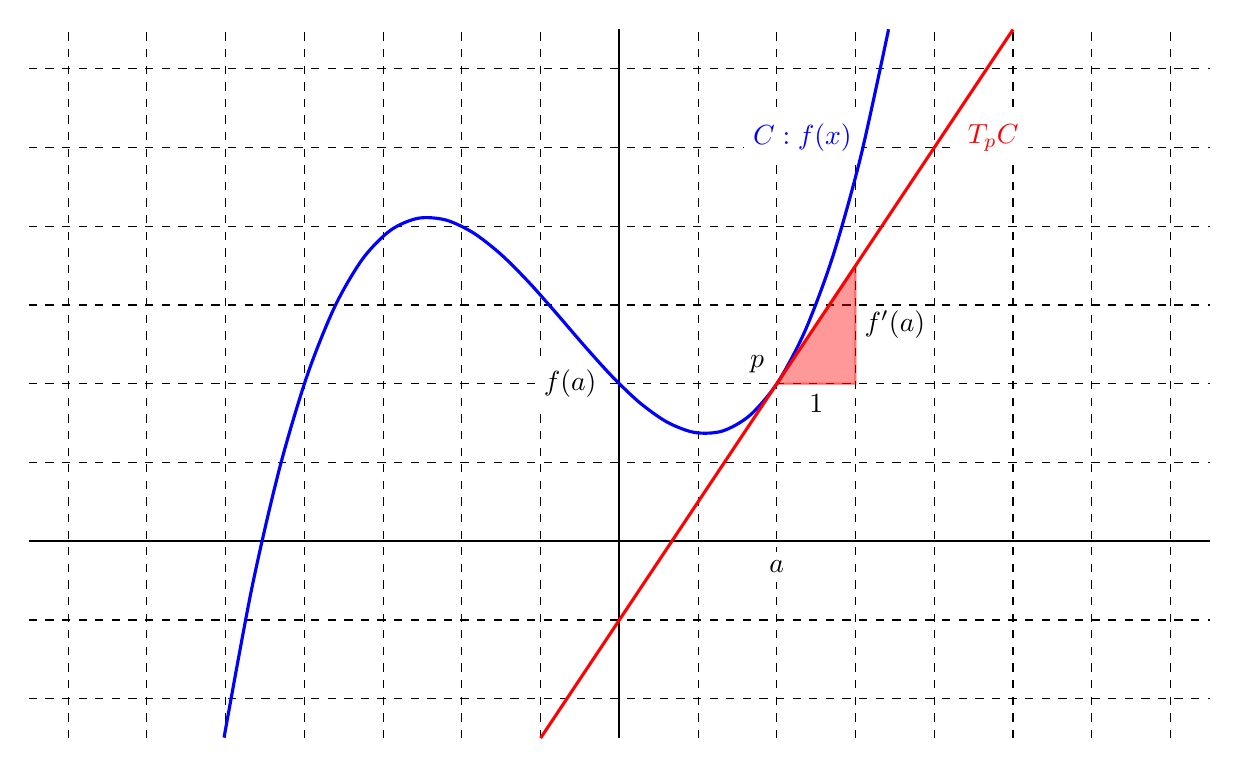
\begin{tikzpicture}
  \draw[thick] (-7.5,0) -- (7.5,0);
  \draw[thick] (0,-2.5) -- (0,6.5);
  \foreach \x in {-7,...,7}
    \draw[dashed] (\x,-2.5) -- (\x,6.5);
  \foreach \y in {-2,...,6}
    \draw[dashed] (-7.5,\y) -- (7.5,\y);

  \node[fill=white] at (-0.625,2) {$f(a)$};
  \node[fill=white] at (2,-0.325) {$a$};
  \node[color=blue,fill=white] at (2.325,5.125) {$C : f(x)$};
  \node[color=red,fill=white]  at (4.75, 5.125) {$T_p C$};
  \filldraw[thick,red,opacity=0.4] (2,2) -- (3,2) -- (3,3.5) -- cycle;
  \draw[line width=0.4mm,blue]   plot[smooth,domain=-5.02:3.42] (\x, {0.125*\x*\x*\x + 0.25*\x*\x - \x + 2});
  \draw[line width=0.4mm,red]   plot[smooth,domain=-1:5] (\x, {1.5*\x - 1});
  
  \node at (2.5,1.75) {$1$};
  \node at (3.5,2.75) {$f'(a)$};
  \node[fill=white] at (1.75,2.25) {$p$};

  %\draw[scale=0.5, domain=-3:3, smooth, variable=\x, blue] plot ({\x}, {\x*\x*\x - \x + 1});
%  \foreach \r in {-4,...,4} {
%    \draw[thick,color=magenta] (-3.25 + \r,-6.5) -- (3.25 + \r,6.5);
%    \node[rotate=90] at (3.25 + \r,7)  {\scriptsize $r = $ \r};
%    \draw[-latex,line width=0.4mm] (0.8*\r + 1, -0.4*\r + 2) -- +(0.4,-0.2);
%    \draw[-latex,line width=0.4mm] (0.8*\r - 1, -0.4*\r - 2) -- +(0.4,-0.2);
%  }
%  \draw[-latex,line width=0.6mm,color=blue] (0,0) -- (3,2);
%  \draw[-latex,line width=0.6mm,color=red] (0,0) -- (0.5,4);
%  \node[color=blue] at (3.25,2) {$\mathbf{v}_1$};
%  \node[color=red] at (0.5,4.25) {$\mathbf{v}_2$};
\end{tikzpicture}
\caption{Illustration of the tangent space of a curve.}
\label{Fig:linearAlgebra_basisSpan_tangentSpace}
\end{center}
\end{figure}

The notion of linear independence and span is connected to geometry and vector calculus as well. For now, let us consider a curve $C$ described by a function $f(x)$. The set of all points along that curve can be described by the pair $(a,f(a))$. We often consider the set of all vectors tangent to the curve at some point $p$ in a local coordinate system with the origin at $p$. This is called the tangent space of curve $C$ at point $p$ denoted by $T_p C$.

Figure~\ref{Fig:linearAlgebra_basisSpan_tangentSpace} gives an illustration. The curve $C$ defined by $f(x)$ is in blue. Suppose the point $p$ is at $x = a, y = f(a)$. We can draw a line in red that is tangent to the curve at $x = a$. Any vector tangent to the curve at $(a,f(a))$ along that line is in the tangent space $T_p C$. Writing this vector component wise can be done by looking at the shaded triangle. Suppose the $x$ component is set to one, then the $y$ component is then the slope, which is obtained from taking the first derivative of $f(x)$ and evaluating it at $x = a$. We can then write the span of $T_p C$ as having a single 2-D vector
\begin{align}
  \text{span} \left\{ 
    \left[ \begin{array}{c} 1 \\  f'(a) \\ \end{array} \right] \right\}
  = c \left[ \begin{array}{c} 1 \\  f'(a) \\ \end{array} \right]  ,
\end{align}
where $c$ is an arbitrary nonzero scalar and $f'(a)$ is the derivative evaluated at $x = a$.

Note that the notion of a tangent space generalizes to higher dimensions. For example, if we have some arbitrary curved 2-D surface in 3-D space, at any point $p$, we can define a plane that is tangent with respect to the surface at that point. The basis of the tangent space in this context contains two linearly independent vectors that reside on the plane. This notion will become important when we study vector calculus.

From these three examples, there is an observation that can be made regarding $\mathbb{R}^3$ a three-dimensional vectors: A span of three linearly independent vectors gives all possible vectors in three-dimensional space; a span of two linearly independent vectors gives the space of all vectors within a plane within $\mathbb{R}^3$; and a span of one linearly independent vector gives the space of all vectors along a line in $\mathbb{R}^3$. These conclusions can be extended to an arbitrary number of dimensions. For example, if we are in $\mathbb{R}^n$, then having a span of $n$ linearly independent vectors gives all vectors in $n$-dimensional space.

These examples described the basis in terms of vectors. The notion of a basis is very general. For example, polynomials can be described using a basis of monomials $x^k$. For example, all quadratic polynomials are spanned by
\begin{align}
  \text{span} \left\{ 1, x, x^2 \right\}
  = a_0 + a_1 x + a_2 x^2 .
\end{align}

%%%%%%%%%%%%%%%%%%%%%%%%%%%%%%%%%%%%%%%%%%%%%%%%%%%%%%%%%%%%%%%%%%%%%%%%%%%%%%%%%%%%%%%%%%%%%%%
\subsection{Example: Quantum Spin and the SU(2) Group}

An example that of a basis that is important in quantum mechanics and the description of spin in an electromagnetic field. This is called the \emph{Special Unity Group} of degree 2 or SU(2). This describes all 2$\times$2 matrices that are unitary (all matrices where the inverse is its conjugate transpose) and have a sum along the diagonal or trace of zero. 

Similar to SU(2), we can describe the space of all 2$\times$2 Hermitian (not necessarily unitary) matrices with zero trace as a linear combination of three 2$\times$2 matrices called the Pauli matrices. Here the Pauli matrices are the basis objects forming the group. The span of these matrices is
\begin{align}
  &\text{span} \left\{ 
    \left[ \begin{array}{c c} 
      0 & 1 \\ 
      1 & 0 \\ \end{array} \right] ,
    \left[ \begin{array}{c c} 
      0 & -i \\ 
      i & 0 \\ \end{array} \right] ,
    \left[ \begin{array}{c c} 
      1 &  0 \\ 
      0 & -1 \\ \end{array} \right] \right\} \nonumber \\
 &= a_1     \left[ \begin{array}{c c} 
      0 & 1 \\ 
      1 & 0 \\ \end{array} \right] 
  + a_2     \left[ \begin{array}{c c} 
      0 & -i \\ 
      i & 0 \\ \end{array} \right]
  + a_3    \left[ \begin{array}{c c} 
      1 &  0 \\ 
      0 & -1 \\ \end{array} \right] \nonumber \\
 &= \left[ \begin{array}{c c} 
      a_3 			&  a_1 - a_2 i \\ 
      a_1 + a_2 i 	& -a_3 			\\ \end{array} \right] .
\end{align}
Here the coefficients $a_k$ are real numbers and $i = \sqrt{-1}$, the imaginary unit. (We call the set of numbers that the coefficients may have the base field.) The resulting matrix is Hermitian because it is equal to its conjugate transpose. Its trace, or sum of the diagonals, is zero since $a_3 - a_3 = 0$.

The resulting matrix times its conjugate transpose is the sum of the squares of the coefficients times the identity matrix:
\begin{align}
 \left[ \begin{array}{c c} 
      a_3 			&  a_1 - a_2 i 	\\ 
      a_1 + a_2 i 	& -a_3 			\\ \end{array} \right] 
    \left[ \begin{array}{c c} 
      a_3 			&  a_1 - a_2 i 	\\ 
      a_1 + a_2 i 	& -a_3 			\\ \end{array} \right]^* 
  = ( a_1^2 + a_2^2 + a_3^2 )     \left[ \begin{array}{c c} 
      1			&  0	\\ 
      0 		& 1		\\ \end{array} \right] .
\end{align}
The matrix is unitary when $a_1^2 + a_2^2 + a_3^2 = 1$. This implies the base field of SU(2) are components of all 3-D real vectors with unit magnitude, which can be geometrically thought of as all vectors that point from the origin to the surface of the unit sphere.

%%%%%%%%%%%%%%%%%%%%%%%%%%%%%%%%%%%%%%%%%%%%%%%%%%%%%%%%%%%%%%%%%%%%%%%%%%%%%%%%%%%%%%%%%%%%%%%
\subsection{Transformation of Vectors and Covectors}

As we saw previously with linear maps, the act of performing matrix multiplication maps one set of vectors to another set. We define a matrix $\mathbf{T}$ as the \emph{forward transformation matrix} that is a tool that can be used to convert basis vectors from one coordinate system to another. Recall that a coordinate system is defined by a set of linearly independent vectors called basis vectors that spans some space (e.g., all real numbers in 3-D space or $\mathbb{R}^3$). The forward transformation matrix $\mathbf{T}$ is constructed by creating a matrix where its columns are the basis vectors of the new coordinate system. 

Note that if we multiply $\mathbf{T}$ onto a matrix containing the standard Cartesian basis vectors $\{ \ihat, \jhat, \khat \}$, which is the identity matrix, then this maps these basis vectors to a new set of basis vectors.

A very simple example is a unit conversion. Suppose in our standard 3-D Cartesian coordinate system we define 1 unit of measurement in each direction to be a foot. Rather, we wish our measurement to be in inches, i.e., in the new coordinate system 1 unit corresponds to 1 inch. To do this, we would need to shorten each basis vector by a factor of 12, since there are 12 inches per foot. The matrix that would do this is a simple scaling on the identity matrix such that all the diagonal elements are $1/12$ and the off-diagonal elements are zero:
\begin{align}
  \mathbf{T} = 
  \left[ \begin{array}{c c c} \rfrac{1}{12} & 0 				& 0  \\
  						      0 			& \rfrac{1}{12} 	& 0  \\
  						      0 			& 0 				& \rfrac{1}{12}  \\ \end{array} \right] . \nonumber 
\end{align}
Let us again emphasize that the matrix $\mathbf{T}$ is called the forward transformation matrix and its purpose is to change the \emph{basis vectors} defining one coordinate system to a set defining another.

We define the forward transformation to be \emph{covariant} with respect to the basis vectors. Said the other way around, the basis vectors change along with (or covary with) the transformation.

A change in the basis or coordinate system does not change the vectors in the sense that we would not expect a purely mathematical operation to change the actual distances, magnitude of the forces, intensities or electric or magnetic fields, etc. If the vector is to remain the same in this sense, then when we change the basis vectors via the forward transformation, we need to adjust the vector components in the precise manner to accomplish this.

Revisiting the example of the conversion from feet to inches. Suppose we have a vector that was 1/2 foot in the $x$ direction, 1 foot in the $y$ direction, and 0 feet in the $z$ direction. Upon doing the change of basis that does the unit conversion by changing the meaning of 1 unit of measurement from a foot to an inch, we would need to convert the vector components from feet to inches. In the new coordinate system, the $x$ component would go from 1/2 foot to 6 inches (or 6 units in the new coordinate system), the $y$ component would go from 1 foot to 12 inches, and the $z$ component would remain at zero. The matrix that accomplishes this via matrix multiplication is a diagonal matrix where all the elements are 12. Note that this is precisely the inverse of $\mathbf{T}$. Therefore, we define a new matrix called the \emph{backward transformation matrix}; which, for our example is
\begin{align}
  \mathbf{T}^{-1} = 
  \left[ \begin{array}{c c c} 12 & 0  & 0  \\
  						      0  & 12 & 0  \\
  						      0  & 0  & 12  \\ \end{array} \right] . \nonumber 
\end{align}
The notion of the backwards transformation matrix for the vector components as the inverse of the forward transformation extends to more complicated coordinate transformations including rotations and skewing.

It bares repeating the key point that a vector is fundamentally unchanged by a change of basis or coordinate transformation. How we measure the vector (i.e., the components) changes to account for the change in basis. The vector components change using the backwards transformation and change against how the basis vectors change to preserve the overall meaning of the vector. We say that the vector components are \emph{contravariant} with respect to the change of basis.

Like vectors, the covectors are fundamentally unchanged by a change of basis, only the covector components. To figure out how, we note that in Cartesian coordinates, the basis covector operating on the basis vector gives
\begin{align}
  \boldsymbol\epsilon_j( \mathbf{e}_i ) = \delta_{ij} = \left\{ \begin{array}{c l} 1 & \quad i = j \\ 0 & \quad i \ne j \\ \end{array} \right. .
\end{align}
Since a change of basis does not impact the vector or covector, merely how they are represented, then this relation must hold in all coordinate systems, i.e., 
\begin{align}
  \boldsymbol\epsilon_j'( \mathbf{e}_i' ) = \boldsymbol\epsilon_j'( \mathbf{T} \mathbf{e}_i ) = \delta_{ij}. 
\end{align}  
To show in 2-D, we can write out the following system:
\begin{subequations}
\begin{align}
  \boldsymbol\epsilon_1'( \mathbf{e}_1' ) &= 
  \left[ \begin{array}{c c} \epsilon_{11}' & \epsilon_{21}' \end{array} \right] 
  \left[ \begin{array}{c c} T_{11} & T_{12} \\ T_{21} & T_{22} \end{array} \right] 
  \left[ \begin{array}{c} 1 \\ 0 \end{array} \right] =
  \left[ \begin{array}{c c} \epsilon_{11}' & \epsilon_{21}' \end{array} \right] 
  \left[ \begin{array}{c} T_{11} \\ T_{21} \end{array} \right] = 1 , \\
%%%%%%
  \boldsymbol\epsilon_1'( \mathbf{e}_2' ) &= 
  \left[ \begin{array}{c c} \epsilon_{11}' & \epsilon_{21}' \end{array} \right] 
  \left[ \begin{array}{c c} T_{11} & T_{12} \\ T_{21} & T_{22} \end{array} \right] 
  \left[ \begin{array}{c} 0 \\ 1 \end{array} \right] =
  \left[ \begin{array}{c c} \epsilon_{11}' & \epsilon_{21}' \end{array} \right] 
  \left[ \begin{array}{c} T_{12} \\ T_{22} \end{array} \right] = 0 , \\
%%%%%%
  \boldsymbol\epsilon_2'( \mathbf{e}_1' ) &= 
  \left[ \begin{array}{c c} \epsilon_{12}' & \epsilon_{22}' \end{array} \right] 
  \left[ \begin{array}{c c} T_{11} & T_{12} \\ T_{21} & T_{22} \end{array} \right] 
  \left[ \begin{array}{c} 1 \\ 0 \end{array} \right] =
  \left[ \begin{array}{c c} \epsilon_{12}' & \epsilon_{22}' \end{array} \right] 
  \left[ \begin{array}{c} T_{11} \\ T_{21} \end{array} \right] = 0 , \\
%%%%%%
  \boldsymbol\epsilon_2'( \mathbf{e}_1' ) &= 
  \left[ \begin{array}{c c} \epsilon_{12}' & \epsilon_{22}' \end{array} \right] 
  \left[ \begin{array}{c c} T_{11} & T_{12} \\ T_{21} & T_{22} \end{array} \right] 
  \left[ \begin{array}{c} 0 \\ 1 \end{array} \right] =
  \left[ \begin{array}{c c} \epsilon_{12}' & \epsilon_{22}' \end{array} \right] 
  \left[ \begin{array}{c} T_{12} \\ T_{22} \end{array} \right] = 1 .
\end{align}
\end{subequations}
The first and second equations can be combined, as can the third and fourth to write the system:
\begin{subequations}
\begin{align}
  \left[ \begin{array}{c c} \epsilon_{11}' & \epsilon_{21}' \end{array} \right] 
  \left[ \begin{array}{c c} T_{11} & T_{12} \\ T_{21} & T_{22} \end{array} \right] =
  \left[ \begin{array}{c c} 1 & 0 \end{array} \right] =
  \left[ \begin{array}{c c} \epsilon_{11} & \epsilon_{21} \end{array} \right], \\
%%%%%%
  \left[ \begin{array}{c c} \epsilon_{12}' & \epsilon_{22}' \end{array} \right] 
  \left[ \begin{array}{c c} T_{11} & T_{12} \\ T_{21} & T_{22} \end{array} \right] =
  \left[ \begin{array}{c c} 0 & 1 \end{array} \right] =
  \left[ \begin{array}{c c} \epsilon_{12} & \epsilon_{22} \end{array} \right] .
\end{align}
\end{subequations}
The backward transformation $\mathbf{T}^{-1}$ may be multiplied on the right, to show the relationship
\begin{align}
  \boldsymbol\epsilon' = \boldsymbol\epsilon \mathbf{T}^{-1}.
\end{align}
This result generalizes to any dimensionality. In other words, to transform the basis covectors, we apply the backward transform, which is opposite to how the basis vectors transform. Therefore, the basis covectors transform contravariantly with respect to the transformation of the basis vectors.

Since, the covectors are not changed under a coordinate transformation and basis covectors transform with the inverse transform, then the covector components must transform with the forward transformation. The covector components transform covariantly with respect to the basis vectors.

To provide a concrete example, let us consider the covector and the two vectors in Sec.~\ref{Sec:linearAlgebra_Covectors_CovectorsAndMatrixMultiplication} on covectors and matrix multiplication:
\begin{align}
  \boldsymbol\alpha &= \left[ \begin{array}{c c} 1 & \rfrac{-1}{2} \\ \end{array} \right] , \hspace{1cm}
  \mathbf{v}_1 = \left[ \begin{array}{c} 3 \\ 2 \\ \end{array} \right] , \hspace{1cm} 
  \mathbf{v}_2 = \left[ \begin{array}{c} \rfrac{1}{2} \\ 4 \\ \end{array} \right]. \nonumber
\end{align}
Now we will apply the (forward) transformation matrix
\begin{align}
  \mathbf{T} = \left[ \begin{array}{c c} 1 & -1 \\ \rfrac{3}{2} & 0 \end{array} \right] . \nonumber
\end{align}
The backwards transformation matrix is its inverse:
\begin{align}
  \mathbf{T}^{-1} = \left[ \begin{array}{c c} 0 & \rfrac{2}{3} \\  -1 & \rfrac{2}{3} \end{array} \right] . \nonumber
\end{align}
The \emph{components} of the vectors $\mathbf{v}_1$ and $\mathbf{v}_2$ transform contravariantly with respect to the basis vectors and therefore use the backwards transform:
\begin{align}
  \mathbf{v}_1' 
  &= \left[ \begin{array}{c c} 0 & \rfrac{2}{3} \\  -1 & \rfrac{2}{3} \end{array} \right] \left[ \begin{array}{c} 3 \\ 2 \\ \end{array} \right] 
   = \left[ \begin{array}{c} \rfrac{4}{3} \\ \rfrac{-5}{3} \\ \end{array} \right], \nonumber \\
%%%%%
  \mathbf{v}_2' 
  &= \left[ \begin{array}{c c} 0 & \rfrac{2}{3} \\  -1 & \rfrac{2}{3} \end{array} \right] \left[ \begin{array}{c} \rfrac{1}{2} \\ 4 \\ \end{array} \right]
   = \left[ \begin{array}{c} \rfrac{8}{3} \\ \rfrac{13}{6} \\ \end{array} \right]. \nonumber
\end{align}
The \emph{components} of the covector $\boldsymbol\alpha$ transform covariantly with respect to the basis vectors and use the forward transformation matrix:
\begin{align}
  \boldsymbol\alpha' 
  = \left[ \begin{array}{c c} 1 & \rfrac{-1}{2} \\ \end{array} \right] \left[ \begin{array}{c c} 1 & -1 \\ \rfrac{3}{2} & 0 \end{array} \right]
  = \left[ \begin{array}{c c} \rfrac{1}{4} & -1 \end{array} \right] . \nonumber
\end{align}
Multiplying the covector and the two vectors in the transformed space gives:
\begin{align}
  \boldsymbol\alpha'( \mathbf{v}_1' ) 
  &= \left[ \begin{array}{c c} \rfrac{1}{4} & -1 \end{array} \right] \left[ \begin{array}{c} \rfrac{4}{3} \\ \rfrac{-5}{3} \\ \end{array} \right]
   = 2, \nonumber \\
%%%%%  
  \boldsymbol\alpha'( \mathbf{v}_2' ) 
  &= \left[ \begin{array}{c c} \rfrac{1}{4} & -1 \end{array} \right] \left[ \begin{array}{c} \rfrac{8}{3} \\ \rfrac{13}{6} \\ \end{array} \right]
   = \rfrac{-3}{2}. \nonumber 
\end{align}
This result is identical to the one from the untransformed coordinate system, which is expected since coordinate transformations do not fundamentally change the vectors and covectors, only their representation.

\begin{figure}[htb!]
\begin{center}
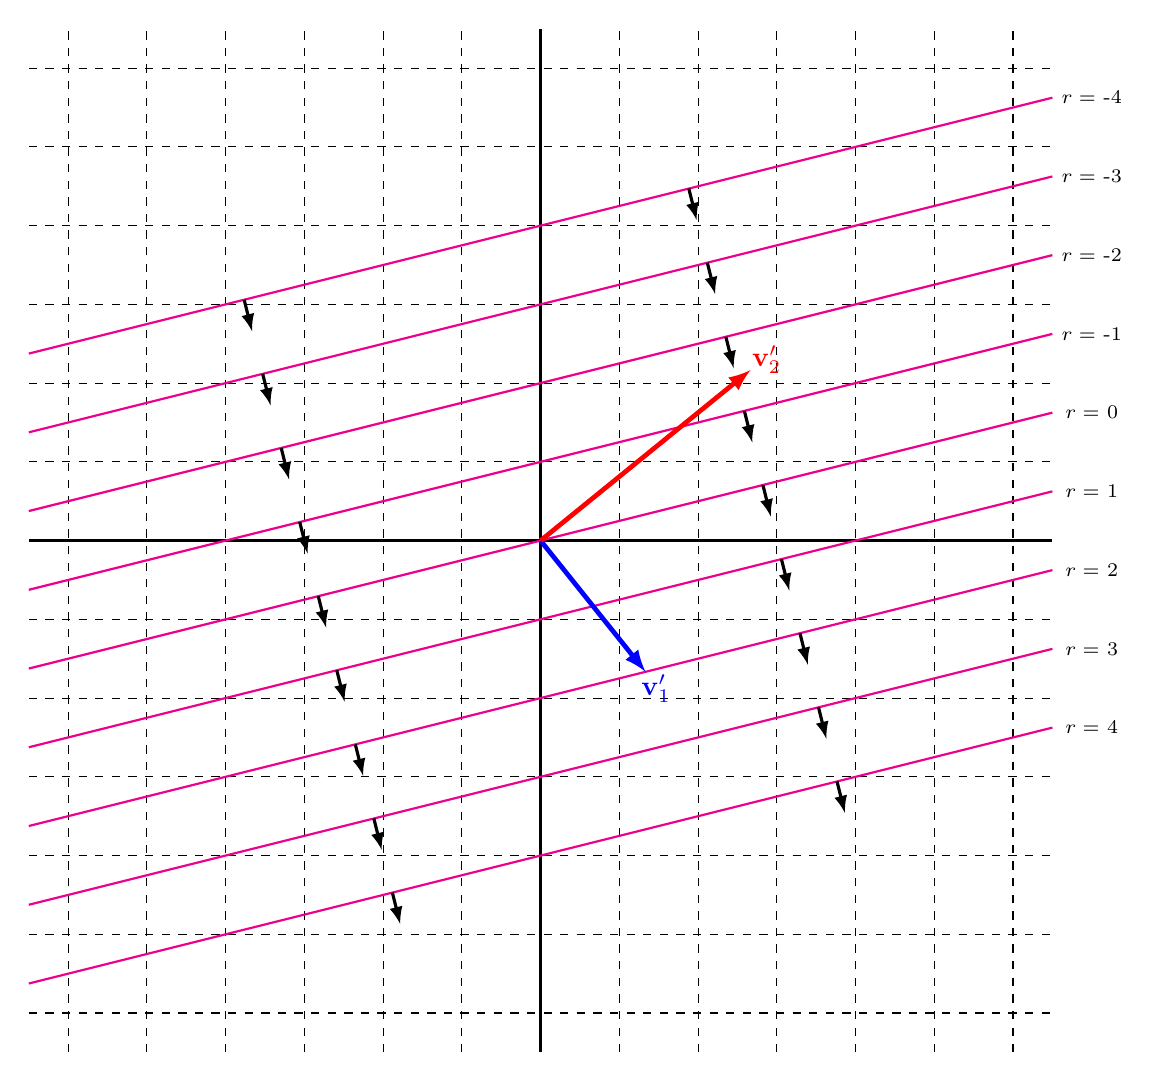
\begin{tikzpicture}
  \draw[thick] (-6.5,0) -- (6.5,0);
  \draw[thick] (0,-6.5) -- (0,6.5);
  \foreach \x in {-6,...,6}
    \draw[dashed] (\x,-6.5) -- (\x,6.5);
  \foreach \y in {-6,...,6}
    \draw[dashed] (-6.5,\y) -- (6.5,\y);
  \foreach \r in {-4,...,4} {
    \draw[thick,color=magenta] (-6.5,-6.5/4 - \r) -- (6.5,6.5/4 - \r);
    \node at (7,6.5/4 - \r)  {\scriptsize $r = $ \r};
%    \draw[thick,color=magenta] (6.5/4 + 3,-6.5) -- (-6.5/4 + 3,6.5);
    \draw[-latex,line width=0.4mm] (4/17*\r + 48/17, -16/17*\r + 12/17) -- +(0.1,-0.4);
    \draw[-latex,line width=0.4mm] (4/17*\r - 48/17, -16/17*\r - 12/17) -- +(0.1,-0.4);
%    \draw[-latex,line width=0.4mm] (4/15*\r + 48/15, -17/4*\r - 21/4) -- +(0.4,-0.2);
  }
  \draw[-latex,line width=0.6mm,color=blue] (0,0) -- (4/3,-5/3);
  \draw[-latex,line width=0.6mm,color=red] (0,0) -- (8/3,13/6);
  \node[color=blue] at ({-4/5*(-5/3-1/6)},{-5/4*(4/3+1/6)}) {$\mathbf{v}_1'$};
  \node[color=red] at ({16/13*(13/6+1/6)},{13/16*(8/3+1/6)}) {$\mathbf{v}_2'$};
\end{tikzpicture}
\caption{Illustration of the vectors and a covector in transformed coordinate system.}
\label{Fig:linearAlgebra_vectorAndCovectorIllustrationTransformedCoordinates}
\end{center}
\end{figure}

An illustration of the vectors and the covector in the transformed coordinate system is given in Fig.~\ref{Fig:linearAlgebra_vectorAndCovectorIllustrationTransformedCoordinates}, similar to what was provided for the untransformed coordinate system (Fig.~\ref{Fig:linearAlgebra_vectorAndCovectorIllustration}). The representation of the vectors in this coordinate system is different, having them both rotated and shortened. The covector is also rotated, but the contour lines are slightly more spread out than in the untransformed coordinate system. Per the result above, both the length of the vectors measured with respect to the covectors are the same in either coordinate system.

This result illustrates an important point in physics: the choice of coordinate system is completely arbitrary and the physical laws and the results we obtain applying them should be identical. For example, the distance traveled between two points should not depend on the coordinate system we choose. If we think of the covector acting on a vector as a measure such a distance, then we expect to get the same results either way and in any other coordinate system. 

The key points from this section may be summarized as follows:
\begin{enumerate}
  \item Neither vectors nor covectors are fundamentally changed by a coordinate transformation or change of basis, merely their representation through the components and basis vectors/covectors;
  \item The \emph{basis vectors} transform \emph{covariantly} with respect to themselves and transform using the \emph{forward transformation matrix}, while the \emph{vector components} transform \emph{contravariantly} with respect to the basis vectors and transform using the \emph{backward transformation matrix}; 
  \item The \emph{basis covectors} transform \emph{contravariantly} with respect to the basis vectors and transform using the \emph{backward transformation matrix}, while the \emph{covector components} transform \emph{covariantly} with respect to the basis vectors and transform using the \emph{forward transformation matrix}.
\end{enumerate}

%\subsection{Transformation of Covectors}
%
%Recall that basis vectors used the forward transform $\mathbf{T}$ and vector components transform contravariant to the basis vectors and use the backward transform $\mathbf{T}^{-1}$. Covectors, on the other hand are opposite. The basis covectors transform contravariant to the basis vectors and the covector components transform in a \emph{covariant} manner with respect to the basis vectors.
%
%To illustrate this, let us apply the following simple transformation matrix:
%\begin{align}
%  \mathbf{T} = 
%  \left[ \begin{array}{c c} 2 & 0   \\
%  						    0 & 2   \\ \end{array} \right] . \nonumber 
%\end{align}
%This transformation scales the basis vectors by a factor of two. Figure~\ref{Fig:linearAlgebra_CovectorTransformation} displays the transformed coordinate space from Fig.~\ref{Fig:linearAlgebra_vectorAndCovectorIllustration}. Notice here the black dashed lines denoting the grid points are now more spread out. (The untransformed grid lines are in light gray for illustration.)
%
%
%\begin{figure}[htb!]
%\begin{center}
%\begin{tikzpicture}
%%  \foreach \x in {-7,...,7}
%%    \draw[dashed,color=gray!50] (\x,-6.5) -- (\x,6.5);
%%  \foreach \y in {-6,...,6}
%%    \draw[dashed,color=gray!50] (-7.5,\y) -- (7.5,\y);
%  \draw[thick] (-7.5,0) -- (7.5,0);
%  \draw[thick] (0,-6.5) -- (0,6.5);
%%%%
%  \foreach \x in {-6,-4,-2,0,2,4,6}
%    \draw[dashed] (\x,-6.5) -- (\x,6.5);
%  \foreach \y in {-6,-4,-2,0,2,4,6}
%    \draw[dashed] (-7.5,\y) -- (7.5,\y);
%  \foreach \r in {-4,...,4} {
%    \draw[thick,color=magenta] (-3.25 + \r,-6.5) -- (3.25 + \r,6.5);
%    \node at (3.25 + \r,6.75)  {\scriptsize $r = $ \r};
%    \draw[-latex,line width=0.4mm] (0.8*\r + 1, -0.4*\r + 2) -- +(0.4,-0.2);
%    \draw[-latex,line width=0.4mm] (0.8*\r - 1, -0.4*\r - 2) -- +(0.4,-0.2);
%  }
%  \draw[-latex,line width=0.6mm,color=blue] (0,0) -- (3,2);
%  \draw[-latex,line width=0.6mm,color=red] (0,0) -- (0.5,4);
%  \node[color=blue] at (3.25,2) {$\mathbf{v}_1$};
%  \node[color=red] at (0.5,4.25) {$\mathbf{v}_2$};
%\end{tikzpicture}
%\caption{Effect of transformation on covectors.}
%\label{Fig:linearAlgebra_CovectorTransformation}
%\end{center}
%\end{figure}
%
%%\begin{figure}[htb!]
%%\begin{center}
%%\begin{tikzpicture}
%%  \foreach \x in {-4,...,4}
%%    \draw[dashed,color=gray!50] (\x,-4.5) -- (\x,4.5);
%%  \foreach \y in {-4,...,4}
%%    \draw[dashed,color=gray!50] (-4.5,\y) -- (4.5,\y);
%%  \draw[thick] (-4.5,0) -- (4.5,0);
%%  \draw[thick] (0,-4.5) -- (0,4.5);
%%%%%
%%  \foreach \x in {-4,-2,0,2,4}
%%    \draw[dashed] (\x,-4.5) -- (\x,4.5);
%%  \foreach \y in {-4,-2,0,2,4}
%%    \draw[dashed] (-4.5,\y) -- (4.5,\y);
%%  \foreach \r in {-2,0,2} {
%%    \draw[thick,color=magenta] (-2.25 + \r,-4.5) -- (2.25 + \r,4.5);
%%    \foreach \s in {0.5*\r}
%%      \node at (2.25 + \r,4.75)  {\scriptsize $r = $ \pgfmathparse{0.5*\r)}\pgfmathprintnumber[precision=1]{\pgfmathresult}};
%%    \draw[-latex,line width=0.4mm] (0.8*\r + 1, -0.4*\r + 2) -- +(0.4,-0.2);
%%    \draw[-latex,line width=0.4mm] (0.8*\r - 1, -0.4*\r - 2) -- +(0.4,-0.2);
%%  }
%%  \draw[-latex,line width=0.6mm,color=blue] (0,0) -- (3,2);
%%  \draw[-latex,line width=0.6mm,color=red] (0,0) -- (0.5,4);
%%  \node[color=blue] at (3.25,2) {$\mathbf{v}_1'$};
%%  \node[color=red] at (0.5,4.25) {$\mathbf{v}_2'$};
%%\end{tikzpicture}
%%\caption{Effect of transformation on covectors.}
%%\label{Fig:linearAlgebra_CovectorTransformation}
%%\end{center}
%%\end{figure}
%
%
%To transform the vector components, we require the backward transformation. This is
%\begin{align}
%  \mathbf{T}^{-1} = 
%  \left[ \begin{array}{c c} \rfrac{1}{2} & 0   			\\
%  						      0 		 & \rfrac{1}{2}  \\  \end{array} \right] . \nonumber 
%\end{align}
%The vectors $\mathbf{v}_1$ and $\mathbf{v}_2$ have their components transformed with the backward transformation:
%\begin{align}
%  \mathbf{v}_1' &= 
%  \left[ \begin{array}{c c} \rfrac{1}{2} 	& 0 			\\
%  						      0 		  	& \rfrac{1}{2} 	\\ \end{array} \right] 
%   \left[ \begin{array}{c} 3 \\ 2 \\ \end{array} \right] =  \left[ \begin{array}{c} \rfrac{3}{2} \\ 1 \\ \end{array} \right]	\nonumber \\	
%%%%%
%  \mathbf{v}_2' &= 
%  \left[ \begin{array}{c c} \rfrac{1}{2} 	& 0 			\\
%  						      0 		  	& \rfrac{1}{2} 	\\ \end{array} \right] 
%   \left[ \begin{array}{c} \rfrac{1}{2} \\ 4 \\ \end{array} \right] =  \left[ \begin{array}{c} \rfrac{1}{4} \\ 2 \\ \end{array} \right]	. \nonumber 
%\end{align}
%The two vectors $\mathbf{v}_1'$ and $\mathbf{v}_2'$ are plotted in Fig.~\ref{Fig:linearAlgebra_CovectorTransformation}. 
%
%Notice that while the vector components are different, the vectors themselves are unchanged by a change of coordinates. The same can be be said about the covectors: the covectors do not change under a change of coordinates, but their components do.


%%%%%%%%%%%%%%%%%%%%%%%%%%%%%%%%%%%%%%%%%%%%%%%%%%%%%%%%%%%%%%%%%%%%%%%%%%%%%%%%%%%%%%%%%%%%%%%
\subsection{Distance, Angles and the Metric Tensor}

The distance we calculate between two points should be the same regardless of our choice of basis. The same applies for the orientation between different objects, i.e., the angles. First, we will focus on the distance calculation, derive an object called the metric tensor, and finally discuss its application to finding angles between vectors.

Two points can be connected with a vector and its length squared can be determined by the dot product of a vector with itself. To illustrate in 2D, the length squared is
\begin{align} \label{Eqn:linearAlgebra_LengthSquared2D}
  r^2 = \mathbf{a} \cdot \mathbf{a} &= ( a_1 \mathbf{e}_1 + a_2 \mathbf{e}_2 ) \cdot ( a_1 \mathbf{e}_1 + a_2 \mathbf{e}_2 ) \nonumber \\
  &= a_1^2 ( \mathbf{e}_1 \cdot \mathbf{e}_1 ) + a_2^2 ( \mathbf{e}_2 \cdot \mathbf{e}_2 ) + 2 a_1 a_2 ( \mathbf{e}_1 \cdot \mathbf{e}_2 ).
\end{align}
For the special case of the Cartesian coordinate system where $\mathbf{e}_1 = \ihat$ and $\mathbf{e}_2 = \jhat$,  we end up with $r^2 = x^2 + y^2$, which is the Pythagorean theorem. (Recall $\ihat \cdot \ihat = 1, \jhat \cdot \jhat = 1, \ihat \cdot \jhat = 0$.) In any other coordinate system, the dot products need to be evaluated properly. As an example, recall the transformed coordinates earlier in this section where the transformed basis vectors are
\begin{align}
  \mathbf{e}_1 = \left[ \begin{array}{c}  1 \\ \rfrac{3}{2} \end{array} \right] , \hspace{1cm}
  \mathbf{e}_2 = \left[ \begin{array}{c} -1 \\ 0 \end{array} \right] . \nonumber
\end{align}
The dot products are
\begin{align}
  \mathbf{e}_1 \cdot \mathbf{e}_1 &= \rfrac{13}{4}, \nonumber \\
  \mathbf{e}_2 \cdot \mathbf{e}_2 &= 1, \nonumber \\
  \mathbf{e}_1 \cdot \mathbf{e}_2 &= -1. \nonumber
\end{align}
The distance formula for the transformed coordinate space is therefore
\begin{align}
  r^2 = \frac{13}{4} a_1^2  + a_2^2 - 2 a_1 a_2 . \nonumber
\end{align}
Now let's check to see if the length squared is the same in both coordinates. Recall the vector
\begin{align}
  \mathbf{v}_1  = \left[ \begin{array}{c} 3 \\ 2 \\ \end{array} \right] , \hspace{1cm} 
  \mathbf{v}_1' = \left[ \begin{array}{c} \rfrac{4}{3} \\ \rfrac{-5}{3} \\ \end{array} \right]. \nonumber
\end{align}
Applying the dot product to both of these with the appropriate basis vectors gives
\begin{align}
  \mathbf{v}_1 \cdot \mathbf{v}_1   &= 3^2 + 2^2 = 13, \nonumber \\
  \mathbf{v}_1' \cdot \mathbf{v}_1' &= \frac{13}{4} \left( \frac{4}{3} \right)^2  + \left( \frac{-5}{3} \right)^2 - 2 \left( \frac{4}{3} \right) \left( \frac{-5}{3} \right) = 13, \nonumber
\end{align}
which is the expected result.

Equation~\eqref{Eqn:linearAlgebra_LengthSquared2D} for the length squared can be rewritten as
\begin{align}
  r^2 = \left[ \begin{array}{c c} a_1 & a_2 \\ \end{array} \right]
        \left[ \begin{array}{c c} \mathbf{e}_1 \cdot \mathbf{e}_1 & \mathbf{e}_1 \cdot \mathbf{e}_2 \\
      							  \mathbf{e}_2 \cdot \mathbf{e}_1 & \mathbf{e}_2 \cdot \mathbf{e}_2 \\ \end{array} \right]
	    \left[ \begin{array}{c} a_1 \\ a_2 \\ \end{array} \right] .
\end{align}
For the specific example the matrix is
\begin{align}
  \mathbf{g} &= \left[ \begin{array}{c c} \rfrac{13}{4} & -1 \\
      							  		 -1			   & 1  \\ \end{array} \right] . \nonumber
\end{align}

This expression may be generalized to any number of dimensions:
\begin{align}
  r^2 = \left[ \begin{array}{c c c c} a_1 & a_2 & \cdots & a_N \\ \end{array} \right]
        \left[ \begin{array}{c c c c} \mathbf{e}_1 \cdot \mathbf{e}_1 & \mathbf{e}_1 \cdot \mathbf{e}_2 & \cdots & \mathbf{e}_1 \cdot \mathbf{e}_N \\
      							      \mathbf{e}_2 \cdot \mathbf{e}_1 & \mathbf{e}_2 \cdot \mathbf{e}_2 & \cdots & \mathbf{e}_2 \cdot \mathbf{e}_N \\ 
							      	  \vdots & \vdots & \ddots & \vdots \\
								      \mathbf{e}_N \cdot \mathbf{e}_1 & \mathbf{e}_N \cdot \mathbf{e}_2 & \cdots & \mathbf{e}_N \cdot \mathbf{e}_N\end{array} \right]
	    \left[ \begin{array}{c} a_1 \\ a_2 \\ \vdots \\ a_N \end{array} \right] .
\end{align}
The matrix in this expression is called the metric tensor and is denoted by
\begin{align}
  \mathbf{g} &= \left[ \begin{array}{c c c c} \mathbf{e}_1 \cdot \mathbf{e}_1 & \mathbf{e}_1 \cdot \mathbf{e}_2 & \cdots & \mathbf{e}_1 \cdot \mathbf{e}_N \\
      							      		  \mathbf{e}_2 \cdot \mathbf{e}_1 & \mathbf{e}_2 \cdot \mathbf{e}_2 & \cdots & \mathbf{e}_2 \cdot \mathbf{e}_N \\ 
							      	  		  \vdots & \vdots & \ddots & \vdots \\
								      		  \mathbf{e}_N \cdot \mathbf{e}_1 & \mathbf{e}_N \cdot \mathbf{e}_2 & \cdots & \mathbf{e}_N \cdot \mathbf{e}_N\end{array} \right] .
\end{align}
The metric tensor is used (as we have seen) for finding lengths of vectors and (as we will soon show) angles between vectors. Note that the inverse metric tensor $\mathbf{g}^{-1}$ can be used to find lengths and angles between covectors.

To find the angle between two vectors, we again use the dot product. Recall,
\begin{align}
  \cos \theta = \frac{ \mathbf{a} \cdot \mathbf{b} }{ | \mathbf{a} | | \mathbf{b} | }. \nonumber
\end{align}
This can be written in terms of the metric tensor as vector-matrix-vector products as
\begin{align}
  \cos \theta = \frac{ \mathbf{a}^\top \mathbf{g} \mathbf{b} }{ ( \mathbf{a}^\top \mathbf{g} \mathbf{a} )^{1/2} \hspace{0.1cm} ( \mathbf{b}^\top \mathbf{g} \mathbf{b} )^{1/2} }. \nonumber
\end{align}

To explore this, let us find the angle between $\mathbf{v}_1$ and $\mathbf{v}_2$ as well as $\mathbf{v}_1'$ and $\mathbf{v}_2'$ from the example. Recall that
\begin{align}
  \mathbf{v}_2  = \left[ \begin{array}{c} \rfrac{1}{2} \\ 4 \\ \end{array} \right] , \hspace{1cm} 
  \mathbf{v}_2' = \left[ \begin{array}{c} \rfrac{8}{3} \\ \rfrac{13}{6} \\ \end{array} \right]. \nonumber
\end{align}
In the untransformed coordinate system:
\begin{align}
  \theta = \cos^{-1} \left[ \frac{ \mathbf{v}_1 \cdot \mathbf{v}_2 }{ ( \mathbf{v}_1 \cdot \mathbf{v}_1 )^{1/2} (  \mathbf{v}_2 \cdot \mathbf{v}_2 )^{1/2} } \right] 
         = \cos^{-1} \left[ \frac{ \rfrac{19}{2} }{ ( 13 )^{1/2} \hspace{0.1cm} (  \rfrac{65}{4} )^{1/2} } \right]
  \approx 49.2^\circ. \nonumber
\end{align}
In the transformed coordinate system
\begin{align}
  \theta = \cos^{-1} \left[ \frac{ \mathbf{v}_1' \cdot \mathbf{v}_2' }{ ( \mathbf{v}_1' \cdot \mathbf{v}_1' )^{1/2} (  \mathbf{v}_2' \cdot \mathbf{v}_2' )^{1/2} } \right] . \nonumber
\end{align}
We have already showed $\mathbf{v}_1' \cdot \mathbf{v}_1' = \mathbf{v}_1 \cdot \mathbf{v}_1 = 13$. It reasons that if the other two dot products are identical, then we will calculate the same angle. Now, using the metric tensor,
\begin{align}
  \mathbf{v}_1' \cdot \mathbf{v}_2' &= 
  		\left[ \begin{array}{c c} \rfrac{4}{3} & \rfrac{-5}{3} \\ \end{array} \right]
        \left[ \begin{array}{c c} \rfrac{13}{4} & -1 \\
      							  		 -1		& 1  \\ \end{array} \right]
	    \left[ \begin{array}{c} \rfrac{8}{3} \\ \rfrac{13}{6} \\ \end{array} \right] = \frac{19}{2}. \nonumber \\
%%%%
  \mathbf{v}_2' \cdot \mathbf{v}_2' &= 
  		\left[ \begin{array}{c c} \rfrac{8}{3} & \rfrac{13}{6} \\ \end{array} \right]
        \left[ \begin{array}{c c} \rfrac{13}{4} & -1 \\
      							  		 -1		& 1  \\ \end{array} \right]
	    \left[ \begin{array}{c} \rfrac{8}{3} \\ \rfrac{13}{6} \\ \end{array} \right] = \frac{65}{4}, \nonumber
\end{align}
we see that indeed the dot products are same, yielding the same angle. In comparing the plots of the vectors in the two coordinate systems in Figs.~\ref{Fig:linearAlgebra_vectorAndCovectorIllustration} and~\ref{Fig:linearAlgebra_vectorAndCovectorIllustrationTransformedCoordinates}, the angles between the two vectors on both plots do not appear identical. If one were to naively calculate the angle in the transformed coordinate without considering the metric tensor, one would get $90.4^\circ$. This may seem odd, but one has to remember that transformations do not change vectors and covectors themselves, only their representation in a particular basis. So while the two appear different, when appropriate measures of lengths and angles for the coordinate systems basis vectors are used, one will get consistent results.


%%%%%%%%%%%%%%%%%%%%%%%%%%%%%%%%%%%%%%%%%%%%%%%%%%%%%%%%%%%%%%%%%%%%%%%%%%%%%%%%%%%%%%%%%%%%%%%
\subsection{Example: Body-Centered Cubic Lattice}

\begin{figure}[tb!]
\begin{center}
\begin{tikzpicture}[x=1cm, y=1cm, z=-0.5cm, rotate around y=-30]
    % Axes
    \draw[-latex] (0,0,0) -- (6,0,0) node [right] {$x$};
    \draw[-latex] (0,0,0) -- (0,6,0) node [left] {$y$};
    \draw[-latex] (0,0,0) -- (0,0,6) node [left] {$z$};
	% Dots for atoms
	\filldraw (0,0,0) circle (3pt);
	\filldraw (4,0,0) circle (3pt);
	\filldraw (0,4,0) circle (3pt);	
	\filldraw (0,0,4) circle (3pt);	
	\filldraw (4,4,0) circle (3pt);
 	\filldraw (4,0,4) circle (3pt);
	\filldraw (0,4,4) circle (3pt);
	\filldraw (4,4,4) circle (3pt);
	\filldraw (2,2,2) circle (3pt);
    % Vectors
    \draw[-latex, line width=0.6mm,color=blue] (0,0,0) -- (4,0,0) node [above,color=black] {$\mathbf{u}$};
    \draw[-latex, line width=0.6mm,color=blue] (0,0,0) -- (0,4,0) node [left,color=black]  {$\mathbf{v}$};
    \draw[-latex, line width=0.6mm,color=blue] (0,0,0) -- (2,2,2) node [left,color=black]  {$\mathbf{w}$};
    % Ticks
        \foreach \i in {2,4}
    {
    \draw (-0.1,\i,0) -- ++ (0.2,0,0);
    \draw (\i,-0.1,0) -- ++ (0,0.2,0);
    \draw (-0.1,0,\i) -- ++ (0.2,0,0);
    }
    % Dashed lines side atoms
    \draw [loosely dashed]
        (0,4,0) -- (4,4,0) -- (4,0,0)
        (0,0,4) -- (4,0,4) -- (4,0,0)
        (0,0,4) -- (0,4,4) -- (0,4,0)
        (4,0,4) -- (4,4,4) -- (4,4,0)
        (0,4,4) -- (4,4,4);
    % Dashed lines center atom
    \draw [loosely dashed]
        (0,2,0) -- (2,2,0) -- (2,0,0)
        (0,0,2) -- (2,0,2) -- (2,0,0)
        (0,0,2) -- (0,2,2) -- (0,2,0)
        (2,0,2) -- (2,2,2) -- (2,2,0)
        (0,2,2) -- (2,2,2);
%    % Labels
%     \node [right] at (2,2,0) {$\begin{bmatrix}
%                                2\\2\\0
%                               \end{bmatrix}$};
%   \node [below] at (2,0,1) {$\begin{bmatrix}
%                               2\\0\\1
%                              \end{bmatrix}$};
\end{tikzpicture}
\caption{Body-Centered Cubic (BCC) Unit Cell and Basis Vectors.}
\label{Fig:linearAlgebra_bccExample_bccLattice}
\end{center}
\end{figure}

Atoms in solids form grains consisting of regular patterns of atoms called a lattice. It is often convenient to write equations in terms of lattice positions, where the integer values correspond to nominal atom sites within the lattice. In most cases, the coordinate system is nonorthogonal. Many calculations such as computing forces and energies involve computing distances between atoms, and the metric tensor is a useful computational tool to quickly calculate distances.

In this example, we consider the body-centered cubic (BCC) lattice as depicted in Fig.~\ref{Fig:linearAlgebra_bccExample_bccLattice}. The basis vectors connect an atom to its neighboring atoms. For this lattice, the basis vectors (see Fig.~\ref{Fig:linearAlgebra_bccExample_bccLattice}) are
\begin{align}
  \mathbf{u} = \left[ \begin{array}{c} 2 \\ 0 \\ 0 \end{array} \right] , \quad 
  \mathbf{v} = \left[ \begin{array}{c} 0 \\ 2 \\ 0 \end{array} \right] , \quad
  \mathbf{w} = \left[ \begin{array}{c} 1 \\ 1 \\ 1 \end{array} \right] .
\end{align}
The basis vectors $\mathbf{u}$ and $\mathbf{v}$ connect atoms on the same face and the basis vector $\mathbf{w}$ connects the face with the center. It is easy to verify by taking dot products that the basis vectors $\mathbf{u}$ and $\mathbf{v}$ are orthogonal to each other, but the basis vector $\mathbf{w}$ is not orthogonal to $\mathbf{u}$ or $\mathbf{v}$. Also it is important to note that the magnitude of $\mathbf{w}$ differs from the magnitudes of $\mathbf{u}$ and $\mathbf{v}$. Taken together, this implies that the distance between two positions given by lattice coordinates would not be given by anything resembling the standard Euclidian distance.

The metric tensor can be used to derive an expression to calculate the distance between any two points in the coordinate system. We can derive the metric tensor by taking dot products of the basis vectors:
\begin{align}
  \mathbf{g} &= \left[ \begin{array}{c c c} \mathbf{u} \cdot \mathbf{u} & \mathbf{u} \cdot \mathbf{v} & \mathbf{u} \cdot \mathbf{w} \\
      							      		\mathbf{v} \cdot \mathbf{u} & \mathbf{v} \cdot \mathbf{v} & \mathbf{v} \cdot \mathbf{w} \\ 
								      		\mathbf{w} \cdot \mathbf{u} & \mathbf{w} \cdot \mathbf{v} & \mathbf{w} \cdot \mathbf{w} \end{array} \right] 
			  = \left[ \begin{array}{c c c} 4 & 0 & 2 \\
      							      		0 & 4 & 2 \\ 
								      		2 & 2 & 3 \end{array} \right] .
\end{align}
Suppose the distance between two arbitrary points is given by the vector
\begin{align}
  a \mathbf{u} + b \mathbf{v} + c \mathbf{w} , \nonumber
\end{align}
The formula for the distance squared (or, equivalently, the magnitude squared of the vector) is then
\begin{align}
  s^2 	&= \left[ \begin{array}{c c c} a & b & c \\ \end{array} \right]
           \left[ \begin{array}{c c c} 4 & 0 & 2 \\
      							      		0 & 4 & 2 \\ 
								      		2 & 2 & 3 \end{array} \right]
		   \left[ \begin{array}{c} a \\ b \\ c \\ \end{array} \right] \nonumber \\
		&= \left[ \begin{array}{c c c} ( 4a + 2c ) & ( 4b + 2c ) & ( 2a + 2b + 3c ) \\ \end{array} \right]
		   \left[ \begin{array}{c} a \\ b \\ c \\ \end{array} \right] \nonumber \\
		&= 4a^2 + 4b^2 + 3c^2 + 4ac + 4bc .
\end{align}
The first collection of terms looks similar to the Euclidian distance, but with different scaling factors. The last two cross terms are different and arise from the nonorthogonality of the coordinate system.

%%%%%%%%%%%%%%%%%%%%%%%%%%%%%%%%%%%%%%%%%%%%%%%%%%%%%%%%%%%%%%%%%%%%%%%%%%%%%%%%%%%%%%%%%%%%%%%
\subsection{Rotation Matrix}

A common operation involving a change of basis involves rotating the coordinate system. Sometimes reorienting the principal axes can simplify the equations that need to be solved.

In 2-D the forward transformation for the basis vectors of the rotation matrix is
\begin{align}
  \mathbf{R} = \left[ \begin{array}{c c} \cos \theta & -\sin \theta \\ \sin \theta & \cos \theta \\ \end{array} \right] .
\end{align}
The backward transformation is
\begin{align}
  \mathbf{R}^{-1} = \left[ \begin{array}{c c} \cos \theta & \sin \theta \\ -\sin \theta & \cos \theta \\ \end{array} \right] .
\end{align}
Note that $\mathbf{R}^{-1} = \mathbf{R}^\top$. This is true of all valid rotation matrices in any number of dimensions.

\begin{figure}[htb!]
\begin{center}
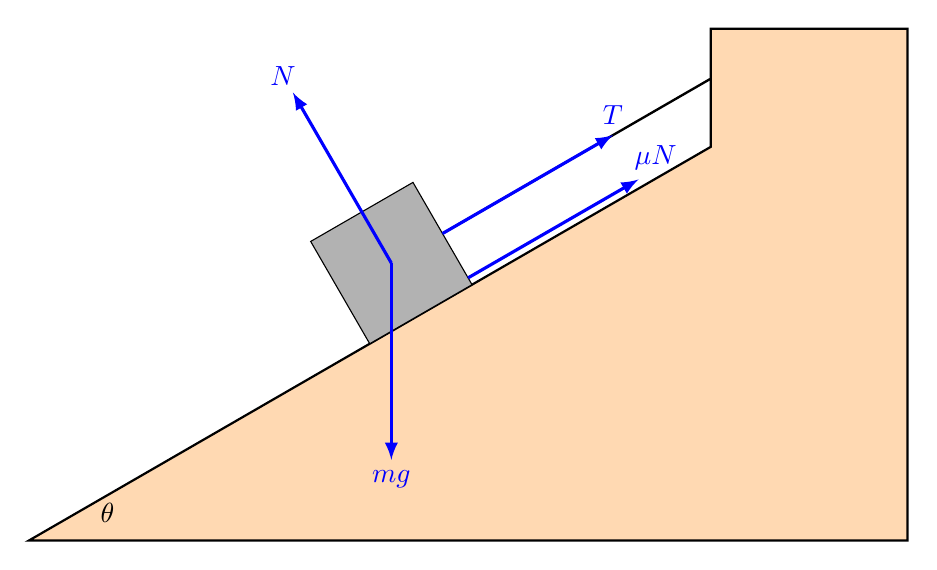
\begin{tikzpicture}
  \draw[thick,fill=orange!30] (0,0) -- ({10*cos(30)},{10*sin(30)}) -- ++(0,1.5) -- ++(2.5,0) -- ++(0,{-1.5 - 10*sin(30)}) -- cycle;
  \draw[fill=gray!60] ({5*cos(30)},{5*sin(30)}) -- ++({1.5*cos(30)},{1.5*sin(30)}) -- ++({1.5*cos(120)},{1.5*sin(120)}) -- ++({-1.5*cos(30)},{-1.5*sin(30)}) -- cycle;
  \draw[line width=0.3mm] ({6.5*cos(30) + 0.75*cos(120)},{6.5*sin(30) + 0.75*sin(120)}) -- ++({3.925*cos(30)},{3.925*sin(30)});
  \node at (1,0.35) {$\theta$};
%%%
  \draw[-latex,line width=0.4mm,color=blue] ({5.75*cos(30) + 0.75*cos(120)},{5.75*sin(30) + 0.75*sin(120)}) -- ++(0,-2.5);
  \node[color=blue] at ({5.75*cos(30) + 0.75*cos(120)},{5.75*sin(30) + 0.75*sin(120) - 2.75}) {$mg$};
%%%%
  \draw[-latex,line width=0.4mm,color=blue] ({5.75*cos(30) + 0.75*cos(120)},{5.75*sin(30) + 0.75*sin(120)}) -- ++({2.5*cos(120)},{2.5*sin(120)});
  \node[color=blue] at ({5.75*cos(30) + 3.5*cos(120)},{5.75*sin(30) + 3.5*sin(120)}) {$N$};
%%%
  \draw[-latex,line width=0.4mm,color=blue] ({6.5*cos(30) + 0.75*cos(120)},{6.5*sin(30) + 0.75*sin(120)}) -- ++({2.5*cos(30)},{2.5*sin(30)});
  \node[color=blue] at ({9.0*cos(30) + 0.75*cos(120)},{9.0*sin(30) + 0.75*sin(120) + 0.25}) {$T$};
%%%
  \draw[-latex,line width=0.4mm,color=blue] ({6.5*cos(30) + 0.1*cos(120)},{6.5*sin(30) + 0.1*sin(120)}) -- ++({2.5*cos(30)},{2.5*sin(30)});
  \node[color=blue] at ({9.25*cos(30) + 0.1*cos(120)},{9.25*sin(30) + 0.1*sin(120) + 0.15}) {$\mu N$};
%%%
\end{tikzpicture}
\caption{Simple statics problem to illustrate rotation matrix.}
\label{Fig:linearAlgebra_staticsExample_RotationMatrix}
\end{center}
\end{figure}

To illustrate where a rotation matrix may be useful, consider the statics problem illustrated in Fig.~\ref{Fig:linearAlgebra_staticsExample_RotationMatrix} where we want to solve for the tension $T$. The force vector components must sum to zero. The force vector is
\begin{align}
  \mathbf{F} = \left[ \begin{array}{c} F_x \\ F_y \\ \end{array} \right] 
  = \left[ \begin{array}{l} T \cos\theta + \mu N \cos\theta - N \sin\theta \\ T \sin\theta + \mu N \sin\theta + N \cos \theta - mg \\ \end{array} \right]
  = \left[ \begin{array}{c} 0 \\ 0  \\ \end{array} \right] . \nonumber
\end{align}
These equations can be simplified considerably if the coordinate system is rotated by angle $\theta$. The components of the force vector transform contravariantly and are transformed using the backwards transformation matrix:
\begin{align}
  \mathbf{R}^{-1} \mathbf{F} = \left[ \begin{array}{c c} \cos \theta & \sin \theta \\ -\sin \theta & \cos \theta \\ \end{array} \right] \left[ \begin{array}{c} F_x \\ F_y \\ \end{array} \right] 
  = \left[ \begin{array}{l} T + \mu N - mg \sin\theta \\ N - mg \cos \theta  \\ \end{array} \right]
  = \left[ \begin{array}{c} 0 \\ 0  \\ \end{array} \right] . \nonumber
\end{align}
The normal force $N$ can be easily eliminated to obtain an expression for the tension:
\begin{align}
  T = mg ( \sin\theta - \mu \cos\theta ) . \nonumber
\end{align}
Now, for a problem such as this, it was probably easier to solve the original equations directly (or to infer the transformed coordinate equations), but this can become considerably more difficult for more complicated problems.

In 3-D rotating about the $x$, $y$, and $z$ axes can be easily deduced. These are:
\begin{subequations}
\begin{align}
  \mathbf{R}_x = \left[ \begin{array}{c c c} 1 & 0 & 0 \\ 0 & \cos \theta & -\sin \theta \\ 0 & \sin \theta & \cos \theta \\ \end{array} \right] , \\
  \mathbf{R}_y = \left[ \begin{array}{c c c} \cos \theta & 0 & \sin \theta \\ 0 & 1 & 0 \\ -\sin \theta & 0 & \cos \theta \\ \end{array} \right] , \\
  \mathbf{R}_z = \left[ \begin{array}{c c c} \cos \theta & -\sin \theta & 0 \\  \sin \theta & \cos \theta & 0 \\ 0 & 0 & 1 \end{array} \right] .
\end{align}
\end{subequations}
Where the backwards transformations are simply the transpose of the matrix. The 3-D general rotation matrix for rotating about an arbitrary axis is complicated to derive, and the derivation is not provided here. Suppose one wishes to rotate an angle $\theta$ about an axis given by vector $\mathbf{u}$, the rotation matrix is
\begin{align}
  \mathbf{R} = \left[ \begin{array}{c c c} 
  \cos\theta + u_x^2 ( 1 - \cos\theta ) 		& u_x u_y ( 1 - \cos\theta ) - u_z \sin\theta 	& u_x u_z ( 1 - \cos\theta ) + u_y \sin\theta 	\\
  u_x u_y ( 1 - \cos\theta ) + u_z \sin\theta 	& \cos\theta + u_y^2 ( 1 - \cos\theta ) 		& u_y u_z ( 1 - \cos\theta ) - u_x \sin\theta 	\\ 
  u_x u_z ( 1 - \cos\theta ) - u_y \sin\theta 	& u_y u_z ( 1 - \cos\theta ) + u_x \sin\theta 	& \cos\theta + u_z^2 ( 1 - \cos\theta ) 		\\ \end{array} \right] .
\end{align}
By setting $\mathbf{u}$ to one of the orthogonal basis vectors, the general 3-D rotation matrix reduces to either of the special cases.


%%%%%%%%%%%%%%%%%%%%%%%%%%%%%%%%%%%%%%%%%%%%%%%%%%%%%%%%%%%%%%%%%%%%%%%%%%%%%%%%%%%%%%%%%%%%%%%
\subsection{Gram-Schmidt Orthogonalization Process} \label{Sec:linearAlgebra_CoordinateSystems_GramSchmidt}

We sometimes find ourselves with a set of linearly independent vectors or basis that are not orthogonal to each other. The question is whether one can devise a scheme to come up with a set of orthogonal vectors. One method of doing this is called the \emph{Gram-Schmidt Orthogonalization Process}. 

Given a set of $k$ vectors $\{ \mathbf{v}_1, \mathbf{v}_2, \ldots , \mathbf{v}_k \}$ (the dimension of the vectors $N$ must be greater than or equal to $k$), we can build the set of $k$ orthogonal vectors $\mathbf{u}$ by
\begin{align}
  \mathbf{u}_1 &= \mathbf{v}_1, \nonumber \\
  \mathbf{u}_2 &= \mathbf{v}_2 - \text{proj}_{ \mathbf{u}_1 }( \mathbf{v}_2 ) , \nonumber \\
  \mathbf{u}_3 &= \mathbf{v}_3 - \text{proj}_{ \mathbf{u}_1 }( \mathbf{v}_3 ) - \text{proj}_{ \mathbf{u}_2 }( \mathbf{v}_3 ) , \nonumber \\
  &\vdots \nonumber \\
  \mathbf{u}_k &= \mathbf{v}_k - \sum_{i=1}^{k-1} \text{proj}_{ \mathbf{u}_i }( \mathbf{v}_k ) .   
\end{align}
The projection operator is defined in Eq.~\eqref{Eqn:linearAlgebra_VectorProjection}. Sometimes it is convenient to rescale the vector $\mathbf{u}_j$ in each step, especially when doing the calculations by hand. This is allowed since a constant scaling does not impact the orthogonality and the projection renormalizes each term anyway. In the same vein, the vectors $\mathbf{u}_j$ are orthogonal, but not naturally normalized; and it is often desired to construct an orthonormal basis:
\begin{align}
  \hat{\mathbf{e}}_j = \frac{ \mathbf{u}_j }{ | \mathbf{u}_j | } .
\end{align}

As an example, consider the space of vectors in $\mathbb{R}^4$ with the following nonorthogonal span:
\begin{align}
  \text{span} \left\{
  \left[ \begin{array}{c}  1 \\  0 \\  1 \\  1 \\ \end{array} \right] ,
  \left[ \begin{array}{c} -1 \\  1 \\  0 \\  0 \\ \end{array} \right] ,
  \left[ \begin{array}{c}  2 \\  1 \\  0 \\  0 \\ \end{array} \right] ,
  \left[ \begin{array}{c}  0 \\  0 \\ -2 \\  1 \\ \end{array} \right] \right\} . \nonumber
\end{align}
We wish to transform to an orthonormal basis using the Gram-Schmidt process.

First, we have simply that
\begin{align}
  \mathbf{u}_1 = \mathbf{v}_1 =  \left[ \begin{array}{c}  1 \\  0 \\  1 \\  1 \\ \end{array} \right] . 
\end{align}
The second orthogonal vector is
\begin{align}
  \mathbf{u}_2 &= \mathbf{v}_2 - \left( \frac{ \mathbf{v}_2 \cdot \mathbf{u}_1 }{ \mathbf{u}_1 \cdot \mathbf{u}_1 } \right) \mathbf{u}_1 
   = \left[ \begin{array}{c} -1 \\  1 \\  0 \\  0 \\ \end{array} \right] + \frac{1}{3} \left[ \begin{array}{c}  1 \\  0 \\  1 \\  1 \\ \end{array} \right]
   = \frac{1}{3}  \left[ \begin{array}{c} -2 \\  3 \\  1 \\  1 \\ \end{array} \right] .
\end{align}
The final form is written with a factor of $\frac{1}{3}$ because scaling does not change the orthogonality. The third orthogonal vector is
\begin{align}
  \mathbf{u}_3 &= \mathbf{v}_3 - \left( \frac{ \mathbf{v}_3 \cdot \mathbf{u}_1 }{ \mathbf{u}_1 \cdot \mathbf{u}_1 } \right) \mathbf{u}_1 
                               - \left( \frac{ \mathbf{v}_3 \cdot \mathbf{u}_2 }{ \mathbf{u}_2 \cdot \mathbf{u}_2 } \right) \mathbf{u}_2 \nonumber \\
   &= \left[ \begin{array}{c} 2 \\  1 \\  0 \\  0 \\ \end{array} \right] 
   - \frac{2}{3}  \left[ \begin{array}{c}  1 \\  0 \\   1 \\  1 \\ \end{array} \right]
   - \frac{1}{15} \left[ \begin{array}{c}  2 \\ -3 \\  -1 \\ -1 \\ \end{array} \right] 
    = \frac{3}{5} \left[ \begin{array}{c}  2 \\  2 \\  -1 \\ -1 \\ \end{array} \right] .
\end{align}
The final orthogonal vector is
\begin{align}
  \mathbf{u}_4 &= \mathbf{v}_4 - \left( \frac{ \mathbf{v}_4 \cdot \mathbf{u}_1 }{ \mathbf{u}_1 \cdot \mathbf{u}_1 } \right) \mathbf{u}_1 
                               - \left( \frac{ \mathbf{v}_4 \cdot \mathbf{u}_2 }{ \mathbf{u}_2 \cdot \mathbf{u}_2 } \right) \mathbf{u}_2 
                               - \left( \frac{ \mathbf{v}_4 \cdot \mathbf{u}_3 }{ \mathbf{u}_3 \cdot \mathbf{u}_3 } \right) \mathbf{u}_3 \nonumber \\
   &= \left[ \begin{array}{c} 0 \\  0 \\ -2 \\  1 \\ \end{array} \right] 
   + \frac{1}{3}  \left[ \begin{array}{c}  1 \\  0 \\   1 \\  1 \\ \end{array} \right]
   - \frac{1}{15} \left[ \begin{array}{c}  2 \\ -3 \\  -1 \\ -1 \\ \end{array} \right] 
   - \frac{1}{10} \left[ \begin{array}{c}  2 \\  2 \\  -1 \\ -1 \\ \end{array} \right]
    = \frac{3}{2} \left[ \begin{array}{c}  0 \\  0 \\  -1 \\  1 \\ \end{array} \right] .
\end{align}
Therefore, an orthogonal basis spanning $\mathbb{R}^4$ based on the original set of vectors is
\begin{align}
  \text{span} \left\{
  \left[ \begin{array}{c}  1 \\  0 \\  1 \\  1 \\ \end{array} \right] ,
  \left[ \begin{array}{c} -2 \\  3 \\  1 \\  1 \\ \end{array} \right] ,
  \left[ \begin{array}{c}  2 \\  2 \\ -1 \\ -1 \\ \end{array} \right] ,
  \left[ \begin{array}{c}  0 \\  0 \\ -1 \\  1 \\ \end{array} \right] \right\} . \nonumber
\end{align}
To find an orthonormal basis, we divide each vector by its respective magnitude:
\begin{align}
  \hat{\mathbf{e}}_1 = \frac{1}{\sqrt{3}}  \left[ \begin{array}{c}  1 \\  0 \\  1 \\  1 \\ \end{array} \right] , \quad
  \hat{\mathbf{e}}_2 = \frac{1}{\sqrt{15}} \left[ \begin{array}{c} -2 \\  3 \\  1 \\  1 \\ \end{array} \right] , \quad
  \hat{\mathbf{e}}_3 = \frac{1}{\sqrt{10}} \left[ \begin{array}{c}  2 \\  2 \\ -1 \\ -1 \\ \end{array} \right] , \quad
  \hat{\mathbf{e}}_4 = \frac{1}{\sqrt{2}}  \left[ \begin{array}{c}  0 \\  0 \\ -1 \\  1 \\ \end{array} \right]  . 
\end{align}


%%%%%%%%%%%%%%%%%%%%%%%%%%%%%%%%%%%%%%%%%%%%%%%%%%%%%%%%%%%%%%%%%%%%%%%%%%%%%%%%%%%%%%%%%%%%%%%
%%%%%%%%%%%%%%%%%%%%%%%%%%%%%%%%%%%%%%%%%%%%%%%%%%%%%%%%%%%%%%%%%%%%%%%%%%%%%%%%%%%%%%%%%%%%%%%
\section{Systems of Linear Equations}

Many phenomena in science and engineering can be described using systems of linear equations. These include: engineering statics, electrical circuits, and thermodynamics of power conversion cycles. Furthermore, many physical phenomena are explained by partial differential equations, which cannot be solved in general, but can be represented approximately as a system of linear equations.

All linear systems can be written in the form
\begin{align}
  \mathbf{Ax} = \mathbf{b},
\end{align}
where $\mathbf{A}$ is a known matrix of coefficients, $\mathbf{x}$ is a column vector of unknowns, and $\mathbf{b}$ is a known column vector of constant or inhomogeneous terms.

The expanded form for this set of equations is as follows:
\begin{align}
  &a_{1,1} x_1 + a_{1,2} x_2 + \cdots + a_{1,M} x_M = b_1, \nonumber \\
  &a_{2,1} x_1 + a_{2,2} x_2 + \cdots + a_{2,M} x_M = b_2, \nonumber \\
  & \quad \vdots \nonumber \\
  &a_{N,1} x_1 + a_{N,2} x_2 + \cdots + a_{N,M} x_M = b_N,
\end{align}
and written equivalently as
\begin{align}
  \left[ \begin{array}{c c c c} a_{1,1} & a_{1,2} & \cdots & a_{1,M} \\
  								a_{2,1} & a_{2,2} & \cdots & a_{2,M} \\
								\vdots  & \vdots  & \ddots & \vdots  \\
								a_{N,1} & a_{N,2} & \cdots & a_{N,M} \\ \end{array} \right]
  \left[ \begin{array}{c} x_1 \\ x_2 \\ \vdots \\ x_M  \\ \end{array} \right] =
  \left[ \begin{array}{c} b_1 \\ b_2 \\ \vdots \\ b_N  \\ \end{array} \right] .
\end{align}
Here we have a system of $N$ equations with $M$ unknowns. If $N = M$, then the system \emph{might} have a unique solution vector $\mathbf{x}$. It is also possible even if $N = M$ for some the equations to be inconsistent, meaning there is no solution or, alternatively, one or more of the equations could be redundant (linearly dependent) and therefore $\mathbf{x}$ has infinitely many solutions that satisfy these equations. The same can be said if $N > M$, more equations than unknowns. If there are fewer equations than unknowns, then there is insufficient information to uniquely determine $\mathbf{x}$ so there may, at best, be an infinite number of solutions; however, the equations could be inconsistent as well meaning that there are two or more linearly dependent equations that have different results, in which case there is no solution to the linear system.

Recall that matrix multiplication has an interpretation of a linear map or coordinate transformation. A geometric interpretation for $\mathbf{Ax} = \mathbf{b}$ is as follows: for a given $N \times M$ transformation matrix $\mathbf{A}$, find the $M \times 1$ vector, or range of such vectors, $\mathbf{x}$ that, upon applying the transformation to them, results in the $N \times 1$ vector $\mathbf{b}$.

Next we will focus on methods of solving these equations (should a solution exist). The algorithm is called Gauss-Jordan elimination or simply Gaussian elimination. This procedure consists of two major steps. The first, is forward elimination and the second is backward substitution. The geometric interpretation to this process is to transform the basis or coordinate system using matrix operations on $\mathbf{A}$ and $\mathbf{b}$ into an orthonormal basis, or as close to one as possible in cases where there is not a unique solution.

%%%%%%%%%%%%%%%%%%%%%%%%%%%%%%%%%%%%%%%%%%%%%%%%%%%%%%%%%%%%%%%%%%%%%%%%%%%%%%%%%%%%%%%%%%%%%%%
\subsection{Forward Elimination} \label{Sec:linearAlgebra_ForwardElimination}

The goal with forward elimination is to apply a set of linear operations to transform the coefficient matrix into a particular form called \emph{row echelon form}. First, we write our linear system in an augmented form:
\begin{align}
  \left[ \begin{array}{c c c c c | c} a_{1,1} & a_{1,2} & \cdots & a_{1,N-1} & a_{1,N} & b_1 \\
  								      a_{2,1} & a_{2,2} & \cdots & a_{2,N-1} & a_{2,N} & b_2 \\
								      \vdots  & \vdots  & \ddots & \vdots    & \vdots  & \vdots \\
									  a_{N-1,1} & a_{N-1,2} & \cdots & a_{N-1,N-1} & a_{N-1,N} & b_{N-1} \\ 
								      a_{N,1} & a_{N,2} & \cdots & a_{N,N-1} & a_{N,N} & b_N \\ \end{array} \right] . \nonumber
\end{align}
This vertical bar in the augmented form separates out the left- and right-hand sides of the equation. This specific form is where the number of equations matches the number of unknowns.

The goal is to manipulate the matrix to be in row echelon form using elementary row operations. This form requires that the matrix be organized in a descending staircase pattern such that there are zeroes below the pattern. An example of row echelon form for a square matrix is:
\begin{align}
  \left[ \begin{array}{c c c c c | c} c_{1,1} & c_{1,2} & \cdots & c_{1,N-1} 	& c_{1,N}   & d_1 \\
  								      0 	  & c_{2,2} & \cdots & c_{2,N-1} 	& c_{2,N}   & d_2 \\
								      \vdots  & \vdots  & \ddots & \vdots    	& \vdots    & \vdots \\
									  0		  & 0 		& \cdots & c_{N-1,N-1} 	& c_{N-1,N} & d_{N-1} \\ 
								      0 	  & 0 		& \cdots & 0			& c_{N,N}   & d_N \\ \end{array} \right] . \nonumber
\end{align}
In this case, we will see that the matrix has a unique solution provided that all the diagonal elements are nonzero. Should any of them be zero, then there will be infinitely many solutions. 

Another example with actual numbers that is also in row-echelon form for a 4$\times$5 system is
\begin{align}
  \left[ \begin{array}{c c c c c | c} 1		  & 1		&  0		& 2			    & 1			& 1		\\
  								      0 	  & 0		&  1	 	& 1				& 2		   	& 0		\\
									  0		  & 0 		&  0  		& 1			 	& -1	    & 2		\\ 
								      0 	  & 0 		&  0		& 0				&  0	    & 0  	\\ \end{array} \right] . \nonumber
\end{align}
This case has two features that distinguish it from the first. One is that the second row does not have a diagonal matrix in the second column entry. The other is that the fourth column is all zeroes. This is still in row echelon form because the pattern is still a descending staircase and backward substitution is possible. It will turn out this case does not have a unique solution, but rather infinitely many solutions over a space of them that can be defined geometrically (in this specific case a plane in 5-dimensional space).

A similar example where no solution exists is as follows:
\begin{align}
  \left[ \begin{array}{c c c c | c}   1		  & 1		&  -1		& 0			    & 3		\\
  								      0 	  & 1		&  1	 	& 1				& -2	\\
									  0		  & 0 		&  1  		& 2			 	&  0	\\ 
								      0 	  & 0 		&  0		& 0				&  1 	\\ \end{array} \right] . \nonumber
\end{align}
Here, the last row is all zeroes on the left-hand side (all coefficients zero), but the right-hand side is nonzero. This would imply zero equals a nonzero number, which is impossible. This implies that the original system included information that was contradictory.

Note that some authors define row echelon form with the diagonal as one. This is helpful with writing efficient numerical algorithms, but is entirely optional for advancing to backward substitution. 

To accomplish the task of transforming an augmented matrix into row-echelon form, we are permitted to do three operations. Each of these elementary row operations may be performed by multiplying the system $\mathbf{Ax} = \mathbf{b}$ on the left by an equivalent transformation matrix $\mathbf{T}$, i.e., $\mathbf{TAx} = \mathbf{Tb}$. These operations are:
\begin{subequations}
\begin{enumerate}
  \item Swap the position of any two rows; this is simply rewriting the equations in a different order. In geometric terms, this is the same as performing a rotation that swaps the coordinate axes.  An example of a $4 \times 4$ transformation matrix that swaps the second and fourth rows is
  \begin{align}
     \mathbf{T} = \left[ \begin{array}{c c c c} 
       1 &  0 &  0 &  0 \\
       0 &  0 &  0 &  1 \\
       0 &  0 &  1 &  0 \\
       0 &  1 &  0 &  0 \\ \end{array} \right] . 
  \end{align}
  This matrix is similar to the identity matrix, except that the location of the ones have been swapped. Here the 1 in the second row is in the fourth column and the 1 in the fourth row is in the second column. This yields the appropriate swap.
  \item Scale any equation by a constant, non-zero factor; this is multiplying both sides of the equation by a constant. An example of a different $4 \times 4$ matrix that scales the second row by a factor of 2 is
  \begin{align}
     \mathbf{T} = \left[ \begin{array}{c c c c} 
       1 &  0 &  0 &  0 \\
       0 &  2 &  0 &  0 \\
       0 &  0 &  1 &  0 \\
       0 &  0 &  0 &  1 \\ \end{array} \right] . 
  \end{align}
  This is similar to the identity matrix except that there is a 2 as opposed to a 1 in the diagonal entry of the second row. This scales the coordinate system along the second coordinate axis.
  \item Replace an equation with a linear combination of that equation and another equation. For example, if we want to replace the third equation by the sum of that equation and 4 times the first equation, the transformation is
  \begin{align}
     \mathbf{T} = \left[ \begin{array}{c c c c} 
       1 &  0 &  0 &  0 \\
       0 &  1 &  0 &  0 \\
       4 &  0 &  1 &  0 \\
       0 &  0 &  0 &  1 \\ \end{array} \right] . 
  \end{align}  
  Again, this is similar to the identity matrix except that in the third row, there is a 4 in the first column. When multiplying the third row by the columns of $\mathbf{A}$ this takes 4 times the first element of the column and adds it to the third element to produce the result. The geometric interpretation of this is it rotates and scales one of the coordinate axes.
\end{enumerate}
\end{subequations}
Note that a common mistake is attempting to directly swap columns, which is not allowed. Column swapping cannot also be done by multiplying a matrix on the left, but rather would require one to multiplied on the right. Since $\mathbf{A}$ multiplies the solution vector $\mathbf{x}$ on the left, this right multiplication would have to be to the right of $\mathbf{x}$ and would therefore act on $\mathbf{Ax}$ and the right-hand side vector $\mathbf{b}$ and not on $\mathbf{A}$ itself.

By chaining together elementary transformation matrices $\mathbf{T}_i$, the matrix $\mathbf{A}$ can be transformed into row echelon form and then reduced-row echelon form. Furthermore, if $\mathbf{A}^{-1}$ exists, then it is the result of the products of all the transformations $\mathbf{T}_i$ applied in the appropriate order given by an algorithm that will be discussed shortly. In practice, we do not perform the matrix multiplication for $\mathbf{T}_i$, as it would be too inefficient either to perform by hand or on a computer. Rather, these are given to show the geometric connection between the elementary row operations and changes of basis.

\begin{figure}[b!]
\begin{center}
\noindent \rule{\textwidth}{1pt}
\begin{verbatim}
 1. let k = 1
 2. loop j over the columns of the matrix A in augmented matrix:
 3.   if a(k,j) = 0:
 4.     loop i down the rows from k+1 until a(i,j) != 0 found
 5.     if such an a(i,j) found: 
 6.       swap rows k and i
 7.     else:
 8.       skip to the next column (do not increment k)
 9.   optional: scale row k by 1/a(k,j)
10.   loop i down the rows from k+1 until the last row:
11.     if a(i,j) != 0:
12.       add a(i,j)/a(k,j) times row k to row i
13.   k += 1
14. return modified augmented matrix
\end{verbatim}
\rule{\textwidth}{1pt}
\caption{Algorithm for forward elimination.}
\label{Fig:linearAlgebra_forwardEliminationAlgorithm}
\end{center}
\end{figure}

Using these three operations, we can develop an algorithm for forward elimination, which will be followed by one for backward substitution. The algorithm applied to a square matrix is given in Fig.~\ref{Fig:linearAlgebra_forwardEliminationAlgorithm}. In short, the algorithm loops over the columns and tries to turn all elements in that column below a pivot row \texttt{k} into zeros by replacing an equation on a row with a linear combination of equations. The condition on line 3 handles the case where the pivot element is zero; when this occurs, we need to attempt to perform a swap with another equation. If we cannot find such an equation, we know the system does not have a unique solution, but we move onto the next column keeping the pivot point \texttt{k} fixed and start there. If we can get the pivot element to be nonzero, we then proceed and make the elements in the current column below that point zero by replacing an equation with a linear combination of that equation and the equation of the pivot row. 

Note that this a mechanical algorithm that will always work, but is not necessarily the most efficient way. When doing forward elimination by hand, it is often beneficial to make heuristic simplifications to make the process more efficient.

%%%%%%%%%%%%%%%%%%%%%%%%%%%%%%%%%%%%%%%%%%%%%%%%%%%%%%%%%%%%%%%%%%%%%%%%%%%%%%%%%%%%%%%%%%%%%%%
\subsubsection{Example 1} 

As an example, consider the following linear system:
\begin{subequations}
\begin{align}
  2y - 1z &= -1, \\ 
  x - 2y &= 0, \\
  3x + y -2z &= 1.
\end{align}
\end{subequations}
This may be represented in matrix-vector form as
\begin{subequations}
\begin{align}
  \left[ \begin{array}{c c c} 
  0 &  2 & -1 \\
  1 & -2 &  0 \\
  3 &  1 & -2 \\ \end{array} \right]
  \left[ \begin{array}{c} x \\ y \\ z \\ \end{array} \right]
  =
  \left[ \begin{array}{c} -1 \\ 0 \\ 1 \\ \end{array} \right] 
\end{align}
or in augmented form as
\begin{align}
  \left[ \begin{array}{c c c | c} 
  0 &  2 & -1 & -1 \\
  1 & -2 &  0 &  0 \\
  3 &  1 & -2 &  1 \\ \end{array} \right] .
\end{align}
To begin the process, start with the first column and go down the rows from $\circled{1}$ to $\circled{3}$ and attempt to make the diagonal terms nonzero and the lower triangle zero. Since the (1,1) element is zero, we must flip this row (equation) with another. Either row $\circled{2}$ or $\circled{3}$ will do, but to be consistent, we will flip rows $\circled{1}$ and $\circled{2}$. The result becomes:
\begin{align}
  \left[ \begin{array}{c c c | c} 
  0 &  2 & -1 & -1 \\
  1 & -2 &  0 &  0 \\
  3 &  1 & -2 &  1 \\ \end{array} \right] 
  : \circled{1} \leftrightarrow \circled{2} : 
  \left[ \begin{array}{c c c | c} 
  1 & -2 &  0 &  0 \\
  0 &  2 & -1 & -1 \\
  3 &  1 & -2 &  1 \\ \end{array} \right] . 
\end{align}
This is merely reordering the equations. Now that we have a non-zero element to work with, we must turn all the elements below the diagonal in the first column to zeroes. The (2,1) element is already zero (as a consequence of the flip), so there remains nothing to be done for row $\circled{2}$. Moving onto row $\circled{3}$, we can eliminate the (3,1) element by subtracting $3$ times row $\circled{1}$ from row $\circled{3}$. This step results in
\begin{align}
  \left[ \begin{array}{c c c | c} 
  1 & -2 &  0 &  0 \\
  0 &  2 & -1 & -1 \\
  3 &  1 & -2 &  1 \\ \end{array} \right] 
  : \circled{3} \rightarrow \circled{3} - 3 \times \circled{1} : 
  \left[ \begin{array}{c c c | c} 
  1 & -2 &  0 &  0 \\
  0 &  2 & -1 & -1 \\
  0 &  7 & -2 &  1 \\ \end{array} \right] 
\end{align}
Now that all elements of the first column below the diagonal are zero, we move onto the second column and do the same using the second row, $\circled{2}$. Next, make the element in the diagonal of the second row 1 by multiplying by $\rfrac{1}{2}$:
\begin{align}
  \left[ \begin{array}{c c c | c} 
  1 & -2 &  0 &  0 \\
  0 &  2 & -1 & -1 \\
  3 &  1 & -2 &  1 \\ \end{array} \right] 
  : \circled{2} \rightarrow \rfrac{1}{2} \times \circled{2} : 
  \left[ \begin{array}{c c c | c} 
  1 & -2 &  0 &  0 \\
  0 &  1 & \rfrac{-1}{2} & \rfrac{-1}{2} \\
  0 &  7 & -2 &  1 \\ \end{array} \right] 
\end{align}
This step is not strictly necessary, but will make the subsequent step easier. The (3,2) element is 7 and should be turned to zero. This can be done by subtracting $7$ times row $\circled{2}$ to row $\circled{3}$:
\begin{align}
  \left[ \begin{array}{c c c | c} 
  1 & -2 &  0 &  0 \\
  0 &  1 & \rfrac{-1}{2} & \rfrac{-1}{2} \\
  0 &  7 & -2 &  1 \\ \end{array} \right] 
  : \circled{3} \rightarrow \circled{3} - 7 \times \circled{2} :
  \left[ \begin{array}{c c c | c} 
  1 & -2 &  0 &  0 \\
  0 &  1 & \rfrac{-1}{2} & \rfrac{-1}{2} \\
  0 &  0 & \rfrac{3}{2}  & \rfrac{9}{2} \\ \end{array} \right] .
\end{align}
Now (optionally) multiplying row $\circled{3}$ by $\rfrac{2}{3}$ to remove the fractions and give a one on the diagonal:
\begin{align}
  \left[ \begin{array}{c c c | c} 
  1 & -2 &  0 &  0 \\
  0 &  1 & \rfrac{-1}{2} & \rfrac{-1}{2} \\
  0 &  0 & \rfrac{3}{2}  & \rfrac{9}{2} \\ \end{array} \right] 
  : \circled{3} \rightarrow  \rfrac{2}{3} \times \circled{3} :
  \left[ \begin{array}{c c c | c} 
  1 & -2 &  0 &  0 \\
  0 &  1 & \rfrac{-1}{2} & \rfrac{-1}{2} \\
  0 &  0 &  1 &  3 \\ \end{array} \right] .
\end{align}
\end{subequations}
At this point forward elimination is complete as the system of equations is in row echelon form. All elements below the diagonal are zero and to continue we will proceed with backward substitution in Sec.~\ref{Sec:linearAlgebra_BackwardSubstitution}. Before we discuss this, let us do another couple examples.

%%%%%%%%%%%%%%%%%%%%%%%%%%%%%%%%%%%%%%%%%%%%%%%%%%%%%%%%%%%%%%%%%%%%%%%%%%%%%%%%%%%%%%%%%%%%%%%
\subsubsection{Example 2} 

Another example is as follows:
\begin{subequations}
\begin{align}
    x_1 -  x_2         + 2 x_4 &= 0 \\
                   x_3 -   x_4 &= 0 \\
    x_1        + 2 x_3 +   x_4 &= 1 \\
           x_2         +   x_4 &= 1. 
\end{align}
\end{subequations}
This system may be converted into matrix-vector form
\begin{subequations}
\begin{align}
  \left[ \begin{array}{c c c c} 
   1 & -1 &  0 &  2 \\
   0 &  0 &  1 & -1 \\
   1 &  0 &  2 &  1 \\
   0 &  1 &  0 &  1 \\ \end{array} \right]
  \left[ \begin{array}{c} x_1 \\ x_2 \\ x_3 \\ x_4 \\ \end{array} \right]
  =
  \left[ \begin{array}{c} 0 \\ 0 \\ 1 \\ 1 \\ \end{array} \right] 
\end{align}
or as an augmented matrix
\begin{align}
  \left[ \begin{array}{c c c c | c} 
   1 & -1 &  0 &  2 &  0 \\
   0 &  0 &  1 & -1 &  0 \\
   1 &  0 &  2 &  1 &  1 \\
   0 &  1 &  0 &  1 &  1 \\ \end{array} \right].
\end{align}
To begin, we start with the first column and turn all elements below the diagonal zero. Thankfully the (2,1) and (4,1) elements are already zero, so we only have to do operations on row $\circled{3}$. The (3,1) element can be made zero by subtracting row $\circled{1}$ from $\circled{3}$:
\begin{align}
  \left[ \begin{array}{c c c c | c} 
   1 & -1 &  0 &  2 &  0 \\
   0 &  0 &  1 & -1 &  0 \\
   1 &  0 &  2 &  1 &  1 \\
   0 &  1 &  0 &  1 &  1 \\ \end{array} \right]
  : \circled{3} \rightarrow \circled{3} -  \circled{1} :
  \left[ \begin{array}{c c c c | c} 
   1 & -1 &  0 &  2 &  0 \\
   0 &  0 &  1 & -1 &  0 \\
   0 &  1 &  2 & -1 &  1 \\
   0 &  1 &  0 &  1 &  1 \\ \end{array} \right].
\end{align}
Now that the elements in the first column below the diagonal are all zero, proceed to the second column. Since the diagonal element (2,2) is zero, we search down the column and swap this row with the row with next available non-zero element, which happens to be (3,2):
\begin{align}
  \left[ \begin{array}{c c c c | c} 
   1 & -1 &  0 &  2 &  0 \\
   0 &  0 &  1 & -1 &  0 \\
   0 &  1 &  2 & -1 &  1 \\
   0 &  1 &  0 &  1 &  1 \\ \end{array} \right]
  : \circled{2} \leftrightarrow \circled{3} :
  \left[ \begin{array}{c c c c | c} 
   1 & -1 &  0 &  2 &  0 \\
   0 &  1 &  2 & -1 &  1 \\
   0 &  0 &  1 & -1 &  0 \\
   0 &  1 &  0 &  1 &  1 \\ \end{array} \right].
\end{align}
Now that there is a one on the diagonal of the second column, proceed down the column and make all elements below the diagonal zero. The element (3,2) is zero by virtue of the swap. The (4,2) element can be made zero by subtracting row $\circled{2}$ from row $\circled{4}$:
\begin{align}
  \left[ \begin{array}{c c c c | c} 
   1 & -1 &  0 &  2 &  0 \\
   0 &  1 &  2 & -1 &  1 \\
   0 &  0 &  1 & -1 &  0 \\
   0 &  1 &  0 &  1 &  1 \\ \end{array} \right]
  : \circled{4} \rightarrow  \circled{4} - \circled{2} :
  \left[ \begin{array}{c c c c | c} 
   1 & -1 &  0 &  2 &  0 \\
   0 &  1 &  2 & -1 &  1 \\
   0 &  0 &  1 & -1 &  0 \\
   0 &  0 & -2 &  2 &  0 \\ \end{array} \right].
\end{align}
Proceeding to the third column, there is a nonzero element in (4,3) which can be made zero by adding two times $\circled{3}$ to row $\circled{4}$:
\begin{align}
  \left[ \begin{array}{c c c c | c} 
   1 & -1 &  0 &  2 &  0 \\
   0 &  1 &  2 & -1 &  1 \\
   0 &  0 &  1 & -1 &  0 \\
   0 &  0 & -2 &  2 &  0 \\ \end{array} \right]
  : \circled{4} \rightarrow \circled{4} + 2 \times \circled{3} :
  \left[ \begin{array}{c c c c | c} 
   1 & -1 &  0 &  2 &  0 \\
   0 &  1 &  2 & -1 &  1 \\
   0 &  0 &  1 & -1 &  0 \\
   0 &  0 &  0 &  0 &  0 \\ \end{array} \right].
\end{align}
\end{subequations}
Notice row $\circled{4}$ is now all zeroes. This implies that the last row contains no new information and that one of the equations in the system is redundant or a linear combination of other equations. As we will see, this will imply that there is no unique solution. Rather, as we will discuss shortly, there is a range of vectors that satisfy this linear system. This is as far as one can take forward elimination for this example. Before proceeding with backward substitution, we will discuss the concept of the rank of a matrix, which gives information on whether the system of equations has a unique solution or, if it does not, the nature of the solutions that may satisfy the equations.

%%%%%%%%%%%%%%%%%%%%%%%%%%%%%%%%%%%%%%%%%%%%%%%%%%%%%%%%%%%%%%%%%%%%%%%%%%%%%%%%%%%%%%%%%%%%%%%
\subsubsection{Example 3} 

The final example in this section is the following linear system:
\begin{subequations}
\begin{align}
     x_1 -   x_2                 +   x_5 &=  1, \\
     x_1         + 2 x_3 -   x_4 +   x_5 &=  0, \\
  -2 x_1         +   x_3 +   x_4 +   x_5 &=  0, \\
             x_2 + 2 x_3 -   x_4         &= -1, \\
         - 2 x_2 +   x_3 +   x_4 + 3 x_5 &=  2.     
\end{align}
Writing the coefficient matrix in augmented form gives
\begin{align}
  \left[ \begin{array}{c c c c c | c} 
   1 & -1 &  0 &  0 &  1 &  1 \\
   1 &  0 &  2 & -1 &  1 &  0 \\
  -2 &  0 &  1 &  1 &  1 &  0 \\
   0 &  1 &  2 & -1 &  0 & -1 \\ 
   0 & -2 &  1 &  1 &  3 &  2 \\ \end{array} \right].
\end{align}
As before, we eliminate the non-zero elements in the first column. The (2,1) element can be eliminated by subtracting row $\circled{2}$ from row $\circled{1}$
\begin{align}
  \left[ \begin{array}{c c c c c | c} 
   1 & -1 &  0 &  0 &  1 &  1 \\
   1 &  0 &  2 & -1 &  1 &  0 \\
  -2 &  0 &  1 &  1 &  1 &  0 \\
   0 &  1 &  2 & -1 &  0 & -1 \\ 
   0 & -2 &  1 &  1 &  3 &  2 \\ \end{array} \right]
  : \circled{2} \rightarrow  \circled{2} - \circled{1} :
  \left[ \begin{array}{c c c c c | c} 
   1 & -1 &  0 &  0 &  1 &  1 \\
   0 &  1 &  2 & -1 &  0 & -1 \\
  -2 &  0 &  1 &  1 &  1 &  0 \\
   0 &  1 &  2 & -1 &  0 & -1 \\ 
   0 & -2 &  1 &  1 &  3 &  2 \\ \end{array} \right].
\end{align}
The (3,1) element can be eliminated by adding twice row $\circled{1}$ to row $\circled{3}$:
\begin{align}
  \left[ \begin{array}{c c c c c | c} 
   1 & -1 &  0 &  0 &  1 &  1 \\
   0 &  1 &  2 & -1 &  0 & -1 \\
  -2 &  0 &  1 &  1 &  1 &  0 \\
   0 &  1 &  2 & -1 &  0 & -1 \\ 
   0 & -2 &  1 &  1 &  3 &  2 \\ \end{array} \right]
  : \circled{3} \rightarrow  \circled{3} + 2 \times \circled{1} :
  \left[ \begin{array}{c c c c c | c} 
   1 & -1 &  0 &  0 &  1 &  1 \\
   0 &  1 &  2 & -1 &  0 & -1 \\
   0 & -2 &  1 &  1 &  3 &  2 \\
   0 &  1 &  2 & -1 &  0 & -1 \\ 
   0 & -2 &  1 &  1 &  3 &  2 \\ \end{array} \right].
\end{align}
The elements of the first column are now all zero below the diagonal, so we move onto the second column. Making the (3,2) element zero is done by adding twice row $\circled{2}$ to row $\circled{3}$:
\begin{align}
  \left[ \begin{array}{c c c c c | c} 
   1 & -1 &  0 &  0 &  1 &  1 \\
   0 &  1 &  2 & -1 &  0 & -1 \\
   0 & -2 &  1 &  1 &  3 &  2 \\
   0 &  1 &  2 & -1 &  0 & -1 \\ 
   0 & -2 &  1 &  1 &  3 &  2 \\ \end{array} \right]
  : \circled{3} \rightarrow  \circled{3} + 2 \times \circled{2} :
  \left[ \begin{array}{c c c c c | c} 
   1 & -1 &  0 &  0 &  1 &  1 \\
   0 &  1 &  2 & -1 &  0 & -1 \\
   0 &  0 &  5 & -1 &  3 &  0 \\
   0 &  1 &  2 & -1 &  0 & -1 \\ 
   0 & -2 &  1 &  1 &  3 &  2 \\ \end{array} \right].
\end{align}
Eliminating the (4,2) element can be done by subtracting row $\circled{2}$ from row $\circled{4}$:
\begin{align}
  \left[ \begin{array}{c c c c c | c} 
   1 & -1 &  0 &  0 &  1 &  1 \\
   0 &  1 &  2 & -1 &  0 & -1 \\
   0 &  0 &  5 & -1 &  3 &  0 \\
   0 &  1 &  2 & -1 &  0 & -1 \\ 
   0 & -2 &  1 &  1 &  3 &  2 \\ \end{array} \right]
  : \circled{4} \rightarrow  \circled{4} - \circled{2} :
  \left[ \begin{array}{c c c c c | c} 
   1 & -1 &  0 &  0 &  1 &  1 \\
   0 &  1 &  2 & -1 &  0 & -1 \\
   0 &  0 &  5 & -1 &  3 &  0 \\
   0 &  0 &  0 &  0 &  0 &  0 \\ 
   0 & -2 &  1 &  1 &  3 &  2 \\ \end{array} \right].
\end{align}
Note that row $\circled{4}$ are now all zeros, indicating that the original equation is a linear combination of at least two other equations. Continuing to eliminate (5,2) by adding twice row $\circled{2}$ to row $\circled{5}$:
\begin{align}
  \left[ \begin{array}{c c c c c | c} 
   1 & -1 &  0 &  0 &  1 &  1 \\
   0 &  1 &  2 & -1 &  0 & -1 \\
   0 &  0 &  5 & -1 &  3 &  0 \\
   0 &  0 &  0 &  0 &  0 &  0 \\ 
   0 & -2 &  1 &  1 &  3 &  2 \\ \end{array} \right]
  : \circled{4} \rightarrow  \circled{4} + 2 \times \circled{2} :
  \left[ \begin{array}{c c c c c | c} 
   1 & -1 &  0 &  0 &  1 &  1 \\
   0 &  1 &  2 & -1 &  0 & -1 \\
   0 &  0 &  5 & -1 &  3 &  0 \\
   0 &  0 &  0 &  0 &  0 &  0 \\ 
   0 &  0 &  5 & -1 &  3 &  0 \\ \end{array} \right].
\end{align}
It should now be apparent that row $\circled{5}$ is identical to row $\circled{3}$, but for the sake of following an programmed algorithm, move onto the third column and scale row $\circled{3}$ by $\rfrac{1}{5}$ to make the diagonal element one:
\begin{align}
  \left[ \begin{array}{c c c c c | c} 
   1 & -1 &  0 &  0 &  1 &  1 \\
   0 &  1 &  2 & -1 &  0 & -1 \\
   0 &  0 &  5 & -1 &  3 &  0 \\
   0 &  0 &  0 &  0 &  0 &  0 \\ 
   0 &  0 &  5 & -1 &  3 &  0 \\ \end{array} \right]
  : \circled{3} \rightarrow  \rfrac{1}{5} \times \circled{3} :
  \left[ \begin{array}{c c c c c | c} 
   1 & -1 &  0 &  0 &  1 &  1 \\
   0 &  1 &  2 & -1 &  0 & -1 \\
   0 &  0 &  1 & -\rfrac{1}{5} &  \rfrac{3}{5} &  0 \\
   0 &  0 &  0 &  0 &  0 &  0 \\ 
   0 &  0 &  5 & -1 &  3 &  0 \\ \end{array} \right].
\end{align}
Finally, eliminate (5,3) by subtracting 5 times row $\circled{3}$ from row $\circled{5}$:
\begin{align}
  \left[ \begin{array}{c c c c c | c} 
   1 & -1 &  0 &  0 &  1 &  1 \\
   0 &  1 &  2 & -1 &  0 & -1 \\
   0 &  0 &  1 & -\rfrac{1}{5} &  \rfrac{3}{5} &  0 \\
   0 &  0 &  0 &  0 &  0 &  0 \\ 
   0 &  0 &  5 & -1 &  3 &  0 \\ \end{array} \right]
  : \circled{5} \rightarrow  \circled{5} - 5 \times \circled{3} :
  \left[ \begin{array}{c c c c c | c} 
   1 & -1 &  0 &  0 &  1 &  1 \\
   0 &  1 &  2 & -1 &  0 & -1 \\
   0 &  0 &  1 & -\rfrac{1}{5} &  \rfrac{3}{5} &  0 \\
   0 &  0 &  0 &  0 &  0 &  0 \\ 
   0 &  0 &  0 &  0 &  0 &  0 \\ \end{array} \right].
\end{align}
\end{subequations}
This matrix is in now in row-echelon form. Note that we now have two rows of zeros meaning that two of the equations were entirely redundant. In the next sections, we will see that this implies there is no unique solution as well.



%First, however, let us do another example:
%\begin{subequations}
%\begin{align}
%  2 x_1 - x_2 + x_3 &= 0 \\
%  5 x_2 + x_3 - 2 x_4 &= 0 \\
%  - x_1 + 3 x_2 - x_4 &= 0 \\
%  2 x_2 - x_3 + 3 x_4 &= 1 . 
%\end{align}
%\end{subequations}
%This system may be converted into matrix-vector form
%\begin{subequations}
%\begin{align}
%  \left[ \begin{array}{c c c c} 
%   2 & -1 &  1 &  0 \\
%   0 &  5 &  1 &  2 \\
%  -1 &  3 &  0 & -1 \\
%   0 &  2 & -1 &  3 \\ \end{array} \right]
%  \left[ \begin{array}{c} x_1 \\ x_2 \\ x_3 \\ x_4 \\ \end{array} \right]
%  =
%  \left[ \begin{array}{c} 0 \\ 0 \\ 0 \\ 1 \\ \end{array} \right] 
%\end{align}
%or as an augmented matrix
%\begin{align}
%  \left[ \begin{array}{c c c c | c} 
%   2 & -1 &  1 &  0 &  0 \\
%   0 &  5 &  1 &  2 &  0 \\
%  -1 &  3 &  0 & -1 &  0 \\
%   0 &  2 & -1 &  3 &  1 \\ \end{array} \right] .
%\end{align}
%To begin, we start with the first column and turn all elements below the diagonal zero. Thankfully the (2,1) and (4,1) elements are already zero, so we only have to do operations on row $\circled{3}$. The (3,1) element can be made zero by adding $\rfrac{1}{2}$ times row $\circled{1}$ to row $\circled{3}$:
%\begin{align}
%  \left[ \begin{array}{c c c c | c} 
%   2 & -1 &  1 &  0 &  0 \\
%   0 &  5 &  1 & -2 &  0 \\
%  -1 &  3 &  0 & -1 &  0 \\
%   0 &  2 & -1 &  3 &  1 \\ \end{array} \right]
%  : \circled{3} \rightarrow \circled{3} + \rfrac{1}{2} \times \circled{1} :
%  \left[ \begin{array}{c c c c | c} 
%   2 & -1 &  1 &  0 &  0 \\
%   0 &  5 &  1 & -2 &  0 \\
%   0 &  \rfrac{5}{2} & \rfrac{1}{2} & -1 &  0 \\
%   0 &  2 & -1 &  3 &  1 \\ \end{array} \right] .
%\end{align}
%Scaling row $\circled{3}$ by a factor of 2 gives:
%\begin{align}
%  \left[ \begin{array}{c c c c | c} 
%   2 & -1 &  1 &  0 &  0 \\
%   0 &  5 &  1 &  -2 &  0 \\
%   0 &  \rfrac{5}{2} & \rfrac{1}{2} & -1 &  0 \\
%   0 &  2 & -1 &  3 &  1 \\ \end{array} \right]
%  : \circled{3} \rightarrow 2 \times \circled{3} :
%  \left[ \begin{array}{c c c c | c} 
%   2 & -1 &  1 &  0 &  0 \\
%   0 &  5 &  1 & -2 &  0 \\
%   0 &  5 &  1 & -2 &  0 \\
%   0 &  2 & -1 &  3 &  1 \\ \end{array} \right] .
%\end{align}
%Now, observe that rows $\circled{2}$ and $\circled{3}$ are identical. This implies the system of equations is redundant, and we know that this system with the provided information does not have a unique solution. Nonetheless, let us proceed by subtracting row $\circled{2}$ from row $\circled{3}$:
%\begin{align}
%  \left[ \begin{array}{c c c c | c} 
%   2 & -1 &  1 &  0 &  0 \\
%   0 &  5 &  1 & -2 &  0 \\
%   0 &  5 &  1 & -2 &  0 \\
%   0 &  2 & -1 &  3 &  1 \\ \end{array} \right]
%  : \circled{3} \rightarrow \circled{3} - \circled{2} :
%  \left[ \begin{array}{c c c c | c} 
%   2 & -1 &  1 &  0 &  0 \\
%   0 &  5 &  1 & -2 &  0 \\
%   0 &  0 &  0 &  0 &  0 \\
%   0 &  2 & -1 &  3 &  1 \\ \end{array} \right] .
%\end{align}
%To make the (4,2) term zero, subtract $\rfrac{2}{5}$ times row $\circled{2}$ from row $\circled{4}$:
%\begin{align}
%  \left[ \begin{array}{c c c c | c} 
%   2 & -1 &  1 &  0 &  0 \\
%   0 &  5 &  1 & -2 &  0 \\
%   0 &  0 &  0 &  0 &  0 \\
%   0 &  2 & -1 &  3 &  1 \\ \end{array} \right]
%  : \circled{4} \rightarrow \circled{4} - \rfrac{2}{5} \times \circled{2} :
%  \left[ \begin{array}{c c c c | c} 
%   2 & -1 &  1 &  0 &  0 \\
%   0 &  5 &  1 & -2 &  0 \\
%   0 &  0 &  0 &  0 &  0 \\
%   0 &  0 & -\rfrac{7}{5} &  \rfrac{19}{5} &  1 \\ \end{array} \right] .
%\end{align}
%Scaling row $\circled{4}$ by 5 gives that row in whole numbers:
%\begin{align}
%  \left[ \begin{array}{c c c c | c} 
%   2 & -1 &  1 &  0 &  0 \\
%   0 &  5 &  1 & -2 &  0 \\
%   0 &  0 &  0 &  0 &  0 \\
%   0 &  0 & -\rfrac{7}{5} &  \rfrac{19}{5} &  1 \\ \end{array} \right] 
%  : \circled{4} \rightarrow 5 \times \circled{2} :
%  \left[ \begin{array}{c c c c | c} 
%   2 & -1 &  1 &  0 &  0 \\
%   0 &  5 &  1 & -2 &  0 \\
%   0 &  0 &  0 &  0 &  0 \\
%   0 &  0 & -7 & 19 &  5 \\ \end{array} \right] .
%\end{align}
%Finally, this may be put into row-echelon form by swapping rows $\circled{3}$ and $\circled{4}$:
%\begin{align}
%  \left[ \begin{array}{c c c c | c} 
%   2 & -1 &  1 &  0 &  0 \\
%   0 &  5 &  1 & -2 &  0 \\
%   0 &  0 &  0 &  0 &  0 \\
%   0 &  0 & -7 & 19 &  5 \\ \end{array} \right] 
%  : \circled{3} \leftrightarrow \circled{4} :
%  \left[ \begin{array}{c c c c | c} 
%   2 & -1 &  1 &  0 &  0 \\
%   0 &  5 &  1 & -2 &  0 \\
%   0 &  0 & -7 & 19 &  5 \\
%   0 &  0 &  0 &  0 &  0 \\ \end{array} \right] .
%\end{align}
%\end{subequations}
%This is as far as one can take forward elimination for this example. Before proceeding with backward substitution, we will discuss the concept of the rank of a matrix, which gives information on whether the system of equations has a unique solution or, if it does not, the nature of the solutions that may satisfy the equations.


%%%%%%%%%%%%%%%%%%%%%%%%%%%%%%%%%%%%%%%%%%%%%%%%%%%%%%%%%%%%%%%%%%%%%%%%%%%%%%%%%%%%%%%%%%%%%%%
\subsection{Matrix Rank}

Before proceeding attempt backward substitution, we need to check something called the rank of the matrix. To find the rank of a matrix, first we must find its row-echelon form. Once this is found, the rank is equal to the number of nonzero rows.

If the rank of the matrix equals the number of rows, then we can assert that there is a unique solution to the system of equations, and it makes sense to proceed with backward substitution. If the rank is less than the number of rows, this implies that there will not be a unique solution. It may be that the equations are inconsistent; in which case there will be no solution. Or it may also be that there are an infinite number of solutions.

For example, if the we find the rank of a 5$\times$5 matrix is 4 and all the equations are consistent, then geometrically, the solution consists of any set of points along a line in 5-D space. Likewise, if the rank of our 5$\times$5 matrix is 3, then the solution corresponds to any point along a plane in that 5-D space.

%%%%%%%%%%%%%%%%%%%%%%%%%%%%%%%%%%%%%%%%%%%%%%%%%%%%%%%%%%%%%%%%%%%%%%%%%%%%%%%%%%%%%%%%%%%%%%%
\subsubsection{Example 1} 

To illustrate, consider the first example from Sec.~\ref{Sec:linearAlgebra_ForwardElimination}:
\begin{align}
  2y - 1z &= -1, \nonumber \\* 
  x - 2y &= 0, \nonumber \\*
  3x + y -2z &= 1. \nonumber
\end{align}
which has the row-echelon form of:
\begin{align}
  \left[ \begin{array}{c c c | c} 
  1 & -2 &  0 &  0 \\
  0 &  1 & \rfrac{-1}{2} & \rfrac{-1}{2} \\
  0 &  0 &  1 &  3 \\ \end{array} \right] . \nonumber
\end{align}
There are three non-zero rows, so the system has a rank of three. Because there are three unknowns, we expect there to be a set of solutions that belong to a $3 - 3 = 0$ dimensional space, or a point in 3-D space. This means that there is one unique set of values that satisfies this system of equations. We say this system is fully determined.

%%%%%%%%%%%%%%%%%%%%%%%%%%%%%%%%%%%%%%%%%%%%%%%%%%%%%%%%%%%%%%%%%%%%%%%%%%%%%%%%%%%%%%%%%%%%%%%
\subsubsection{Example 2} 

Now, let us consider the second example from Sec.~\ref{Sec:linearAlgebra_ForwardElimination}:
\begin{align}
    x_1 -  x_2         + 2 x_4 &= 0 \nonumber \\
                   x_3 -   x_4 &= 0 \nonumber \\
    x_1        + 2 x_3 +   x_4 &= 1 \nonumber \\
           x_2         +   x_4 &= 1. \nonumber
\end{align}
which has a row-echelon form of
\begin{align}
  \left[ \begin{array}{c c c c | c} 
   1 & -1 &  0 &  2 &  0 \\
   0 &  1 &  2 & -1 &  1 \\
   0 &  0 &  1 & -1 &  0 \\
   0 &  0 &  0 &  0 &  0 \\ \end{array} \right] . \nonumber
\end{align}
This has three non-zero rows, and therefore has a rank of three. Since there are four unknowns, we expect the space of solutions to live on a $4-3 = 1$ dimensional space, or a line. It is said that this system is underdetermined in the sense that there is no unique solution, however, we can classify the solution space as a set of vectors that point to anywhere along a line in 4-D space.

It is also possible for a system of equations to be inconsistent, suppose that the last row of the previous example did not have a zero to the right of the vertical bar. This would state that $0 \ne 0$, which is, of course, impossible. Therefore, while the rank is still three, there is no set of numbers that can satisfy all the equations consistently and therefore there is no solution at all.

%%%%%%%%%%%%%%%%%%%%%%%%%%%%%%%%%%%%%%%%%%%%%%%%%%%%%%%%%%%%%%%%%%%%%%%%%%%%%%%%%%%%%%%%%%%%%%%
\subsubsection{Example 3} 

The third example from Sec.~\ref{Sec:linearAlgebra_ForwardElimination} is a system of five equations, 
\begin{align}
     x_1 -   x_2                 +   x_5 &=  1, \nonumber \\
     x_1         + 2 x_3 -   x_4 +   x_5 &=  0, \nonumber \\
  -2 x_1         +   x_3 +   x_4 +   x_5 &=  0, \nonumber \\
             x_2 + 2 x_3 -   x_4         &= -1, \nonumber \\
         - 2 x_2 +   x_3 +   x_4 + 3 x_5 &=  2. \nonumber     
\end{align}
that has the row-echelon form of
\begin{align}
  \left[ \begin{array}{c c c c c | c} 
   1 & -1 &  0 &  0 &  1 &  1 \\
   0 &  1 &  2 & -1 &  0 & -1 \\
   0 &  0 &  1 & -\rfrac{1}{5} &  \rfrac{3}{5} &  0 \\
   0 &  0 &  0 &  0 &  0 &  0 \\ 
   0 &  0 &  0 &  0 &  0 &  0 \\ \end{array} \right]. \nonumber
\end{align}
This has three non-zero rows and is also a rank of three. Since there are five unknowns, the space of solutions lives on a $5-3 = 2$ dimensional space, or a line in 5-D space, assuming the equations are consistent.

%%%%%%%%%%%%%%%%%%%%%%%%%%%%%%%%%%%%%%%%%%%%%%%%%%%%%%%%%%%%%%%%%%%%%%%%%%%%%%%%%%%%%%%%%%%%%%%
\subsection{Backward Substitution} \label{Sec:linearAlgebra_BackwardSubstitution}

If the rank of the matrix (number of non-zero rows) of the row-echelon form of matrix $\mathbf{A}$ is equal to the number of its rows, then there exists a unique solution and we can proceed with doing backward substitution.

Before writing an algorithm, it may be worth seeing an example. A possible system of equations in row-echelon form is as follows:
\begin{align}
  2x_1 + x_2 - x_3  &= -1, \nonumber \\
        -x_2 + 3x_3 &= 1, \nonumber \\
              -2x_3 &= 2. \nonumber
\end{align}
Starting with the third equation we can see
\begin{align}
  x_3 = \frac{2}{-2} = -1. \nonumber
\end{align}
Now we can use the second equation to get
\begin{align}
  x_2 = \frac{1 - 3\cdot(-1)}{-1} = -4. \nonumber
\end{align}
Finally, from the first equation we can write
\begin{align}
  x_1 = \frac{-1 - (-1)\cdot(-1) - (1)\cdot(-4)}{2} = 1. \nonumber
\end{align}
This suggests a general equation for backward substitution
\begin{align}
  x_i = \dfrac{ b_i - \displaystyle\sum_{j=i+1}^N a_{i,j} x_j }{ a_{i,i} }.
\end{align}
An algorithm for this is given in Fig.~\ref{Fig:linearAlgebra_backwardSubstitutionAlgorithm}.

\begin{figure}[htb!]
\begin{center}
\noindent \rule{\textwidth}{1pt}
\begin{verbatim}
 1.	loop i backward over the rows:
 2.	  let s = 0
 3.	  loop j forward over the columns starting from i+1:
 4.	    s += a(i,j)*x(j)
 5.	  x(i) = ( b(i) - s )/a(i,i)
 6.	return x
\end{verbatim}
\rule{\textwidth}{1pt}
\caption{Algorithm for backward substitution.}
\label{Fig:linearAlgebra_backwardSubstitutionAlgorithm}
\end{center}
\end{figure}

%%%%%%%%%%%%%%%%%%%%%%%%%%%%%%%%%%%%%%%%%%%%%%%%%%%%%%%%%%%%%%%%%%%%%%%%%%%%%%%%%%%%%%%%%%%%%%%
\subsubsection{Example 1} 

Continuing with the first example from Sec.~\ref{Sec:linearAlgebra_ForwardElimination}, the row echelon form obtained
\begin{subequations}
\begin{align}
  \left[ \begin{array}{c c c | c} 
  1 & -2 &  0 &  0 \\
  0 &  1 & \rfrac{-1}{2} & \rfrac{-1}{2} \\
  0 &  0 &  1 &  3 \\ \end{array} \right] . 
\end{align}
results in the following system of equations:
\begin{align}
   x - 2y &=  0, \\*
   y - \frac{1}{2} z &= -\frac{1}{2}, \\* 
            z &= 3.
\end{align}
Starting with the third equation in row $\circled{3}$, we can trivially solve for $z$,
\begin{align}
  z = 3.
\end{align}
Substituting this value of $z$ into the second equation in row $\circled{2}$:
\begin{align}
  y = \frac{ -\frac{1}{2} + \frac{1}{2} (3) }{1} = 1.
\end{align}
Finally, substituting $y$ and $z$ into the first equation in row $\circled{1}$ gives the value of $x$:
\begin{align}
  x = \frac{ 0 + 2 (1) }{1} = 2.
\end{align}
Therefore, the solution is
\begin{align} \label{Eqn:linearAlgebra_example1solution}
  \left[ \begin{array}{c} x \\ y \\ z \\ \end{array} \right] =
  \left[ \begin{array}{c} 2 \\ 1 \\ 3 \\ \end{array} \right] .
\end{align}
\end{subequations}
This result yields a single point in 3-D space, which was expected since the rank of the system is 3 and matches the number of unknowns.

%%%%%%%%%%%%%%%%%%%%%%%%%%%%%%%%%%%%%%%%%%%%%%%%%%%%%%%%%%%%%%%%%%%%%%%%%%%%%%%%%%%%%%%%%%%%%%%
\subsubsection{Example 2} 

Moving on to the second example, we obtained the row echelon form of 
\begin{subequations}
\begin{align}
  \left[ \begin{array}{c c c c | c} 
   1 & -1 &  0 &  2 &  0 \\
   0 &  1 &  2 & -1 &  1 \\
   0 &  0 &  1 & -1 &  0 \\
   0 &  0 &  0 &  0 &  0 \\ \end{array} \right]
\end{align}
Since the last row is simply $0 = 0$ and provides no new information, we can simply delete that row:
\begin{align}
  \left[ \begin{array}{c c c c | c} 
   1 & -1 &  0 &  2 &  0 \\
   0 &  1 &  2 & -1 &  1 \\
   0 &  0 &  1 & -1 &  0 \\ \end{array} \right] ,
\end{align}
which is described by the equations
\begin{align}
   x_1 -   x_2         + 2 x_4 &= 0, \\
           x_2 + 2 x_3 -   x_4 &= 1, \\
                   x_3 -   x_4 &= 0.
\end{align}
Since there are only three equations and four unknowns, we cannot have a unique solution. Nonetheless, we may proceed and obtain a set of solutions by applying backward substitution to the first three columns of the linear system. Using the third equation, we can obtain:
\begin{align}
  x_3 = x_4 .
\end{align}
Using the second equation,
\begin{align}
  x_2 + 2 x_4 - x_4 = 1, \nonumber
\end{align}
and solving for $x_2$ gives an expression in terms of $x_4$:
\begin{align}
  x_2 = 1 - x_4 .
\end{align}
Finally, using the first equation,
\begin{align}
  x_1 - ( 1 - x_4 ) + 2 x_4 = 0, \nonumber
\end{align}
and solving for $x_1$ results in the equation
\begin{align}
  x_1 = 1 - 3 x_4.
\end{align}
Rearranging these three equations results in the system:
\begin{align}
  x_1 + 3 x_4 &= 1, \\
  x_2 +   x_4 &= 1, \\
  x_3 -   x_4 &= 0 ,
\end{align}
with the following augmented form
\begin{align}
  \left[ \begin{array}{c c c c | c} 
   1 &  0 &  0 &  3 &  1 \\
   0 &  1 &  0 &  1 &  1 \\
   0 &  0 &  1 & -1 &  0 \\ \end{array} \right] .
\end{align}
Note that this is called the \emph{reduced-row echelon form} of the linear system.

We can also allow $x_4$ to be some free parameter, as in
\begin{align}
  x_4 = \alpha.
\end{align}
Substituting this in and writing as a vector system yields the solution:
\begin{align} \label{Eqn:linearAlgebra_example2solution}
  \left[ \begin{array}{c} x_1 \\ x_2 \\ x_3 \\ x_4 \\ \end{array} \right] =
  \left[ \begin{array}{c} 1 \\ 1 \\ 0  \\ 0 \\ \end{array} \right] +
  \alpha \left[ \begin{array}{c} -3 \\ -1 \\ 1 \\ 1 \\ \end{array} \right] .
\end{align}
\end{subequations}
This describes a line in four dimensional space that contain valid solutions to the linear system of equations.

%%%%%%%%%%%%%%%%%%%%%%%%%%%%%%%%%%%%%%%%%%%%%%%%%%%%%%%%%%%%%%%%%%%%%%%%%%%%%%%%%%%%%%%%%%%%%%%
\subsubsection{Example 3} 

Finally, for the third example, forward elimination yields
\begin{subequations}
\begin{align}
  \left[ \begin{array}{c c c c c | c} 
   1 & -1 &  0 &  0 &  1 &  1 \\
   0 &  1 &  2 & -1 &  0 & -1 \\
   0 &  0 &  1 & -\rfrac{1}{5} &  \rfrac{3}{5} &  0 \\
   0 &  0 &  0 &  0 &  0 &  0 \\ 
   0 &  0 &  0 &  0 &  0 &  0 \\ \end{array} \right]. \nonumber
\end{align}
The final two rows are all zero, providing no information and can be removed,
\begin{align}
  \left[ \begin{array}{c c c c c | c} 
   1 & -1 &  0 &  0 &  1 &  1 \\
   0 &  1 &  2 & -1 &  0 & -1 \\
   0 &  0 &  1 & -\rfrac{1}{5} &  \rfrac{3}{5} &  0 \\ \end{array} \right]. \nonumber
\end{align}
We can write an equation for $x_3$ and solve in terms of $x_4$ and $x_5$:
\begin{align}
  x_3 = \frac{1}{5} x_4 - \frac{3}{5} x_5 .
\end{align}
Solving for $x_2$ in terms of $x_4$ and $x_5$ yields
\begin{align}
  x_2 &= -1 + \frac{3}{5} x_4 + \frac{6}{5} x_5 .
\end{align}
Finally, $x_1$ in terms of $x_4$ and $x_5$ is
\begin{align}
  x_1 &= \frac{3}{5} x_4 + \frac{1}{5} x_5 .
\end{align}
This gives the system
\begin{align}
  x_1 - \frac{3}{5} x_4 - \frac{1}{5} x_5 &=  0, \\
  x_2 - \frac{3}{5} x_4 - \frac{6}{5} x_5 &= -1, \\
  x_3 - \frac{1}{5} x_4 + \frac{3}{5} x_5 &=  0.
\end{align}
Arranging this into the reduced-row echelon form gives
\begin{align}
  \left[ \begin{array}{c c c c c | c} 
   1 &  0 &  0 & -\rfrac{3}{5} & -\rfrac{1}{5} &  0 \\
   0 &  1 &  0 & -\rfrac{3}{5} & -\rfrac{6}{5} & -1 \\
   0 &  0 &  1 & -\rfrac{1}{5} &  \rfrac{3}{5} &  0 \\ \end{array} \right] .
\end{align}
There are two free parameters, so define
\begin{align}
  x_4 &= 5 \alpha, \\
  x_5 &= 5 \beta,
\end{align}
where $\alpha$ and $\beta$ are any real number. Putting the equations into vector form, the solution then is
\begin{align} \label{Eqn:linearAlgebra_example2solution}
  \left[ \begin{array}{c} x_1 \\ x_2 \\ x_3 \\ x_4 \\ x_5 \end{array} \right] =
  \left[ \begin{array}{c} 0 \\ -1 \\ 0  \\ 0 \\ 0 \\ \end{array} \right] +
  \alpha \left[ \begin{array}{c} 3 \\ 3 \\ 1 \\ 5 \\ 0 \end{array} \right] +
  \beta  \left[ \begin{array}{c} 1 \\ 6 \\ -3 \\ 0 \\ 5 \end{array} \right] .
\end{align}
\end{subequations}
This vector equation describes a plane in 5-D space.

%%%%%%%%%%%%%%%%%%%%%%%%%%%%%%%%%%%%%%%%%%%%%%%%%%%%%%%%%%%%%%%%%%%%%%%%%%%%%%%%%%%%%%%%%%%%%%%
\subsection{Discussion of Solutions}

To understand the solution to the first problem geometrically, the original matrix
\begin{align} 
  \mathbf{A} &=
  \left[ \begin{array}{c c c} 
  0 &  2 & -1 \\
  1 & -2 &  0 \\
  3 &  1 & -2 \\ \end{array} \right] \nonumber
\end{align}
can be thought of as a linear transformation that maps a vector $\mathbf{x}$ onto another vector $\mathbf{b}$. In this case, the right-hand side vector is
\begin{align}
  \mathbf{b} &= \left[ \begin{array}{c} -1 \\ 0 \\ 1 \\ \end{array} \right] . \nonumber
\end{align}
The solution to this mapping is unique and given by Eq.~\eqref{Eqn:linearAlgebra_example1solution} as
\begin{align} 
  \mathbf{x} =
  \left[ \begin{array}{c} 2 \\ 1 \\ 3 \\ \end{array} \right] . \nonumber
\end{align}
Multiplying $\mathbf{A}$ by $\mathbf{x}$ yields the vector $\mathbf{b}$. Furthermore, there is only a single mapping of $\mathbf{x}$ onto $\mathbf{b}$, so the linear map given by $\mathbf{A}$ is said to be one-to-one. This also implies that $\mathbf{A}$ is invertible. The solution space is therefore a unique point in 3-D space.

With the second problem, the original matrix
\begin{align} 
  \mathbf{A} &=
  \left[ \begin{array}{c c c c} 
   1 & -1 &  0 &  2 \\
   0 &  0 &  1 & -1 \\
   1 &  0 &  2 &  1 \\
   0 &  1 &  0 &  1 \\ \end{array} \right] \nonumber
\end{align}
maps a vector $\mathbf{x}$ onto another vector
\begin{align}
  \mathbf{b} = \left[ \begin{array}{c} 0 \\ 0 \\ 1 \\ 1 \\ \end{array} \right] \nonumber
\end{align}
and we wish to know which vectors $\mathbf{x}$ would map to this solution $\mathbf{b}$, which are given by the solution in Eq.~\eqref{Eqn:linearAlgebra_example2solution}. Examples of vectors that map to $\mathbf{b}$ lie along a line in 4-D space parameterized by a constant $\alpha$ that may take on any real number. Examples of possible solutions are using $\alpha = 0, -1, 2$ respectively,
\begin{align}
  \left[ \begin{array}{c}  1 \\  1 \\  0  \\  0 \\ \end{array} \right] , \quad 
  \left[ \begin{array}{c}  4 \\  2 \\ -1  \\ -1 \\ \end{array} \right] , \quad
  \left[ \begin{array}{c} -5 \\ -1 \\  2  \\  2 \\ \end{array} \right] . \nonumber
\end{align}
All of these vectors, when multiplied by $\mathbf{A}$ yield the same solution vector $\mathbf{b}$. Correspondingly, the transformation in not one-to-one in that there is no unique mapping of $\mathbf{b}$ to $\mathbf{x}$. This implies that $\mathbf{A}$ is not invertible, i.e., $\mathbf{A}^{-1}$ does not exist.

%%%%%%%%%%%%%%%%%%%%%%%%%%%%%%%%%%%%%%%%%%%%%%%%%%%%%%%%%%%%%%%%%%%%%%%%%%%%%%%%%%%%%%%%%%%%%%%
\subsection{Example: Electrical Circuit}

Electric circuits are important in applications in nuclear engineering. Nuclear power plants convert heat generated from nuclear reactions into electricity that must be then supplied to the grid. A nuclear power plant itself has numerous electric circuits as part of its operation involving sensors and other equipment that must be designed and analyzed. Radiation detectors also involve electronics that are analyzed using electrical circuits. Furthermore, most experiments involve some form of electrical circuitry.

Electric circuits involving batteries (power sources) and resistors can be described by systems of linear algebraic equations, and the methods of writing these systems of equations is provided in this section. Electric circuits involving capacitors and inductors, conversely, result in linear systems of ordinary differential equations, which is the subject of the next chapter.

To analyze electrical circuits involving batteries and resistors, we apply Kirchoff's rules, which states that the electrical potential (voltage) $V$ is equal to the product of the net electrical current $I$ and the resistance $R$. The applied voltage and resistances are generally known, whereas the currents $I$ are not.

\begin{figure}[htp!]
\begin{center}
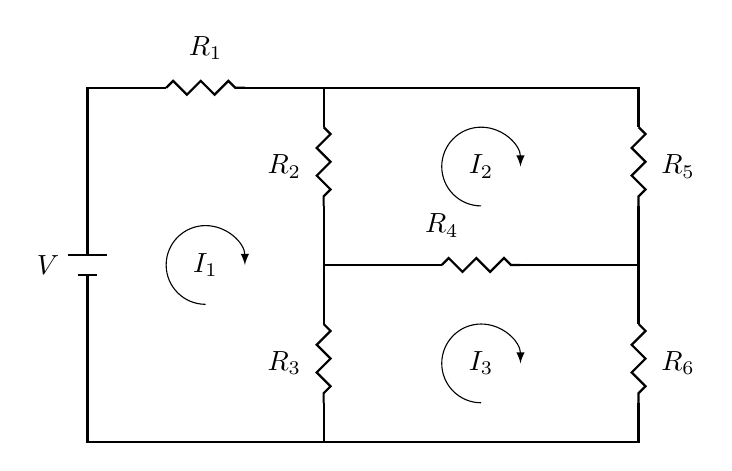
\begin{tikzpicture}
  \draw[thick] (-0.125,-0.125) -- (0.125,-0.125);
  \draw[thick] (-0.25,  0.125) -- (0.25,  0.125);
  \draw[thick] (0,0.125) -- (0,2.25) -- (1,2.25);
  \draw[thick,decorate,decoration=zigzag] (1,2.25) -- (2,2.25);
  \draw[thick] (2,2.25) -- (3,2.25) -- (3,1.75);
  \draw[thick,decorate,decoration=zigzag] (3,1.75) -- (3,0.75); 
  \draw[thick] (3,0.75) -- (3,-0.75);
  \draw[thick,decorate,decoration=zigzag] (3,-0.75) -- (3,-1.75); 
  \draw[thick] (3,-1.75) -- (3,-2.25) -- (0,-2.25) -- (0,-0.125); 
  \node at (-0.5,0) {$V$};
  \node at (1.5,0) {$I_1$};
  \draw[-latex] (1.5,-0.5) arc (270:0:0.5);
  \node at (1.5, 2.75) {$R_1$};
  \node at (2.5, 1.25) {$R_2$};
  \node at (2.5,-1.25) {$R_3$};
%%%%%
  \draw[thick] (3,2.25) -- (7,2.25) -- (7,1.75);
  \draw[thick,decorate,decoration=zigzag] (7,1.75) -- (7,0.75);
  \draw[thick] (7,0.75) -- (7,-0.75); 
  \draw[thick,decorate,decoration=zigzag] (7,-0.75) -- (7,-1.75);
  \draw[thick] (7,-1.75) -- (7,-2.25) -- (3,-2.25);
  \node at (5,1.25) {$I_2$};
  \draw[-latex] (5,0.75) arc (270:0:0.5);
  \node at (4.5,0.5) {$R_4$};
  \node at (7.5,1.25) {$R_5$};
%%%%
  \draw[thick] (3,0) -- (4.5,0);
  \draw[thick,decorate,decoration=zigzag] (4.5,0) -- (5.5,0);
  \draw[thick] (5.5,0) -- (7,0);
  \node at (5,-1.25) {$I_3$};
  \draw[-latex] (5,-1.75) arc (270:0:0.5);
  \node at (7.5,-1.25) {$R_6$};
\end{tikzpicture}
\caption{Example of an electrical circuit diagram.}
\label{Fig:linearAlgebra_electricalCircuit_Example1}
\end{center}
\end{figure}

Consider the following example in Fig.~\ref{Fig:linearAlgebra_electricalCircuit_Example1}. We proceed to write Kirchoff's rule for each loop within the system numbered by the index on the subscript of the current in that loop $I_i$. For the first loop, we write:
\begin{subequations}
\begin{align}
  I_1 R_1 + ( I_1 - I_2 ) R_2 + ( I_1 - I_3 ) R_3 = V.
\end{align}
Each term applies to a resistor in the loop, which are $j = 1, 2, 3$. The current is the net electric current with respect to the loop being analyzed. The first term is $I_1 - 0$ since there is no adjacent loop. For the second term, we must subtract off the current in the second loop. And likewise for the third. Finally, the right-hand side has the voltage applied to the circuit $V$. The second loop has the following equation:
\begin{align}
  ( I_2 - I_1 ) R_2 + ( I_2 - I_3 ) R_4 + I_2 R_5 = 0.
\end{align}
As with the first loop, there is a term for each resistor with the net current multiplied by each. The right-hand side is now zero since there is no applied voltage in this section of the loop. The third loop has the equation
\begin{align}
  ( I_3 - I_1 ) R_3 + ( I_3 - I_2 ) R_4 + I_3 R_6 = 0.
\end{align}
Taking these equations and rearranging to be in terms of the unknown electric currents gives the following linear system:
\begin{align}
  ( R_1 + R_2 + R_3 ) I_1 - R_2 I_2 - R_3 I_3 &= V, \\
  -R_2 I_1 + ( R_2 + R_4 + R_5 ) I_2 - R_4 I_3 &= 0, \\
  -R_3 I_1 - R_4 I_2 + ( R_3 + R_4 + R_6 ) I_3 &= 0.
\end{align}
The resulting matrix-vector form is
\begin{align}
  \left[ \begin{array}{c c c} 
  ( R_1 + R_2 + R_3 ) & -R_2 & -R_3 \\
  -R_2 & ( R_2 + R_4 + R_5 ) & -R_4 \\
  -R_3 & -R_4 &  ( R_3 + R_4 + R_6 ) \\ \end{array} \right]
  \left[ \begin{array}{c} I_1 \\ I_2 \\ I_3 \\ \end{array} \right]
  =
  \left[ \begin{array}{c} V \\ 0 \\ 0 \\ \end{array} \right] .
\end{align}
\end{subequations}
This system of equations can then be solved using Gaussian elimination.

%%%%%%%%%%%%%%%%%%%%%%%%%%%%%%%%%%%%%%%%%%%%%%%%%%%%%%%%%%%%%%%%%%%%%%%%%%%%%%%%%%%%%%%%%%%%%%%
%\subsection{Example: Thermodynamic Power Conversion Cycle}


%%%%%%%%%%%%%%%%%%%%%%%%%%%%%%%%%%%%%%%%%%%%%%%%%%%%%%%%%%%%%%%%%%%%%%%%%%%%%%%%%%%%%%%%%%%%%%%
\subsection{Matrix Inversion} \label{Sec:linearAlgebra_SystemsOfLinearEquations_MatrixInversion}

In Sec.~\ref{Sec:linearAlgebra_Matrices_MatrixInverse} we introduced the inverse of a matrix, but did not discuss how it may be computed except for providing some formulas for 2$\times$2 and diagonal matrices. In this section, we will discuss how to use Gaussian elimination to solve for the matrix inverse. Note that formally, we may solve the linear system equations as 
\begin{align}
  \mathbf{x} = \mathbf{A}^{-1} \mathbf{b}.
\end{align}
Therefore, if we know $\mathbf{A}^{-1}$, we could easily solve for $\mathbf{x}$ for any inhomogeneous column vector $\mathbf{b}$. This being said, it is rare, at least for large systems of equations, that we actually require solving for $\mathbf{A}^{-1}$. Rather Gaussian elimination can be used more efficiently to solve $\mathbf{Ax} = \mathbf{b}$ as we discussed, or, should $\mathbf{A}$ have a specific structure, there may be specialized techniques that can be employed.

Should we actually need to compute $\mathbf{A}^{-1}$, we start by writing the equation of the form
\begin{align}
  \mathbf{A} \mathbf{A}^{-1} = \mathbf{I} .
\end{align}
Here $\mathbf{A}$ is known and its inverse $\mathbf{A}^{-1}$ is not. As with Gaussian elimination, we apply elementary row operations that can be formally described by $\mathbf{T}_i$ on left side in the order according to the algorithm. This removes the matrix $\mathbf{A}$ on the left-hand side leaving the solution for $\mathbf{A}^{-1}$ on the right. Practically, this is done by constructing the augmented matrix of $\mathbf{A}$ with the identity matrix $\mathbf{I}$
\begin{align}
  \left[ \begin{array}{c c c c c | c c c c c} 
    a_{1,1}   & a_{1,2}   & \cdots & a_{1,N-1}   & a_{1,N}   & 1      & 0      & \cdots & 0       & 0      \\
  	a_{2,1}   & a_{2,2}   & \cdots & a_{2,N-1}   & a_{2,N}   & 0      & 1      & \cdots & 0       & 0      \\
	\vdots    & \vdots    & \ddots & \vdots      & \vdots    & \vdots & \vdots & \ddots & \vdots  & \vdots \\
	a_{N-1,1} & a_{N-1,2} & \cdots & a_{N-1,N-1} & a_{N-1,N} & 0      & 0      & \cdots & 1       & 0      \\ 
	a_{N,1}   & a_{N,2}   & \cdots & a_{N,N-1}   & a_{N,N}   & 0      & 0      & \cdots & 0       & 1      \\ 
	\end{array} \right]  \nonumber
\end{align}
in a similar manner to the system $\mathbf{Ax} = \mathbf{b}$. We then use the same three allowed operations, swapping, scaling, and replacing an equation with a linear combination of that equation with another, to arrive at the following augmented matrix:
\begin{align}
  \left[ \begin{array}{c c c c c | c c c c c} 
    1       & 0     & \cdots & 0       & 0      & \widetilde{a}_{1,1}   & \widetilde{a}_{1,2}   & \cdots & \widetilde{a}_{1,N-1}   & \widetilde{a}_{1,N}   \\
  	0      & 1      & \cdots & 0       & 0      & \widetilde{a}_{2,1}   & \widetilde{a}_{2,2}   & \cdots & \widetilde{a}_{2,N-1}   & \widetilde{a}_{2,N}   \\
	\vdots & \vdots & \ddots & \vdots  & \vdots & \vdots                & \vdots                & \ddots & \vdots                  & \vdots                \\
	0      & 0      & \cdots & 1       & 0      & \widetilde{a}_{N-1,1} & \widetilde{a}_{N-1,2} & \cdots & \widetilde{a}_{N-1,N-1} & \widetilde{a}_{N-1,N} \\ 
	0      & 0      & \cdots & 0       & 1      & \widetilde{a}_{N,1}   & \widetilde{a}_{N,2}   & \cdots & \widetilde{a}_{N,N-1}   & \widetilde{a}_{N,N}   \\ 
	\end{array} \right] . \nonumber
\end{align}
Here $\widetilde{a}_{i,j}$ are the coefficients of $\mathbf{A}^{-1}$.

As stated previously, algorithm for finding the matrix inverse first uses forward elimination in the same manner as with the $\mathbf{Ax} = \mathbf{b}$ solve before. The difference arises in that backward substitution is replaced with a second ``backward'' elimination step that mirrors the forward elimination step, except everything is done in reverse. If at any point during the forward elimination process, a row of all zeroes is detected, then the algorithm can stop as the matrix is singular and $\mathbf{A}^{-1}$ does not exist.

As an example, consider the matrix:
\begin{subequations}
\begin{align}
  \mathbf{A} = 
  \left[ \begin{array}{c c c c}
   1 &  0 & -1 &  2 \\
  -1 &  1 &  0 & -1 \\
  -1 &  0 &  1 &  0 \\
   0 &  2 &  1 & -1 \\ \end{array} \right] .
\end{align}
This matrix can be augmented with the identity matrix as follows:
\begin{align}
  \left[ \begin{array}{c c c c | c c c c }
   1 &  0 & -1 &  2 &  1 &  0 &  0 &  0 \\
  -1 &  1 &  0 & -1 &  0 &  1 &  0 &  0 \\
  -1 &  0 &  1 &  0 &  0 &  0 &  1 &  0 \\
   0 &  2 &  1 & -1 &  0 &  0 &  0 &  1 \\ \end{array} \right] .
\end{align}
Our goal is to turn the left side into the identity matrix where the right side becomes the matrix inverse. To do this algorithmically, we perform forward elimination on the left side. For the first column to make (2,1) and (3,1) zero, replace row $\circled{2}$ with the sum of $\circled{2}$ and $\circled{1}$ and $\circled{3}$ with the sum of $\circled{3}$ and $\circled{1}$:
\begin{align}
  &\left[ \begin{array}{c c c c | c c c c }
   1 &  0 & -1 &  2 &  1 &  0 &  0 &  0 \\
  -1 &  1 &  0 & -1 &  0 &  1 &  0 &  0 \\
  -1 &  0 &  1 &  0 &  0 &  0 &  1 &  0 \\
   0 &  2 &  1 & -1 &  0 &  0 &  0 &  1 \\ \end{array} \right]  
   : \circled{2} \rightarrow \circled{2} + \circled{1} : \nonumber \\
  &\left[ \begin{array}{c c c c | c c c c }
   1 &  0 & -1 &  2 &  1 &  0 &  0 &  0 \\
   0 &  1 & -1 &  1 &  1 &  1 &  0 &  0 \\
  -1 &  0 &  1 &  0 &  0 &  0 &  1 &  0 \\
   0 &  2 &  1 & -1 &  0 &  0 &  0 &  1 \\ \end{array} \right] , \\
%%%%%
  &\left[ \begin{array}{c c c c | c c c c }
   1 &  0 & -1 &  2 &  1 &  0 &  0 &  0 \\
   0 &  1 & -1 &  1 &  1 &  1 &  0 &  0 \\
  -1 &  0 &  1 &  0 &  0 &  0 &  1 &  0 \\
   0 &  2 &  1 & -1 &  0 &  0 &  0 &  1 \\ \end{array} \right] 
   : \circled{3} \rightarrow \circled{3} + \circled{1} : \nonumber \\
  &\left[ \begin{array}{c c c c | c c c c }
   1 &  0 & -1 &  2 &  1 &  0 &  0 &  0 \\
   0 &  1 & -1 &  1 &  1 &  1 &  0 &  0 \\
   0 &  0 &  0 &  2 &  1 &  0 &  1 &  0 \\
   0 &  2 &  1 & -1 &  0 &  0 &  0 &  1 \\ \end{array} \right] .
\end{align}
Moving onto the second column, make the (4,2) element zero by replacing row $\circled{4}$ with $\circled{4}$ minus twice $\circled{2}$:
\begin{align}
  &\left[ \begin{array}{c c c c | c c c c }
   1 &  0 & -1 &  2 &  1 &  0 &  0 &  0 \\
   0 &  1 & -1 &  1 &  1 &  1 &  0 &  0 \\
   0 &  0 &  0 &  2 &  1 &  0 &  1 &  0 \\
   0 &  2 &  1 & -1 &  0 &  0 &  0 &  1 \\ \end{array} \right]  
   : \circled{4} \rightarrow \circled{4} - 2 \times \circled{2} : \nonumber \\
  &\left[ \begin{array}{c c c c | c c c c }
   1 &  0 & -1 &  2 &  1 &  0 &  0 &  0 \\
   0 &  1 & -1 &  1 &  1 &  1 &  0 &  0 \\
   0 &  0 &  0 &  2 &  1 &  0 &  1 &  0 \\
   0 &  0 &  3 & -3 & -2 & -2 &  0 &  1 \\ \end{array} \right] .
\end{align}
Moving onto the third column, there is a zero in the (3,3) element, so we move down and swap rows $\circled{3}$ and $\circled{4}$:
\begin{align}
  &\left[ \begin{array}{c c c c | c c c c }
   1 &  0 & -1 &  2 &  1 &  0 &  0 &  0 \\
   0 &  1 & -1 &  1 &  1 &  1 &  0 &  0 \\
   0 &  0 &  0 &  2 &  1 &  0 &  1 &  0 \\
   0 &  0 &  3 & -3 & -2 & -2 &  0 &  1 \\ \end{array} \right]  
   : \circled{3} \leftrightarrow \circled{4} : \nonumber \\
  &\left[ \begin{array}{c c c c | c c c c }
   1 &  0 & -1 &  2 &  1 &  0 &  0 &  0 \\
   0 &  1 & -1 &  1 &  1 &  1 &  0 &  0 \\
   0 &  0 &  3 & -3 & -2 & -2 &  0 &  1 \\
   0 &  0 &  0 &  2 &  1 &  0 &  1 &  0 \\ \end{array} \right] .
\end{align}
This finishes the forward elimination phase. Next, we do the process in reverse, starting at the last column and working up and to the left. First, scale row $\circled{4}$ by $\rfrac{1}{2}$ and row $\circled{3}$ by $\rfrac{1}{3}$:
\begin{align}
  &\left[ \begin{array}{c c c c | c c c c }
   1 &  0 & -1 &  2 &  1 &  0 &  0 &  0 \\
   0 &  1 & -1 &  1 &  1 &  1 &  0 &  0 \\
   0 &  0 &  3 & -3 & -2 & -2 &  0 &  1 \\
   0 &  0 &  0 &  2 &  1 &  0 &  1 &  0 \\ \end{array} \right] 
   : \circled{4} \rightarrow  \rfrac{1}{2} \times \circled{4} : \nonumber \\
  &\left[ \begin{array}{c c c c | c c c c }
   1 &  0 & -1 &  2 &  1 &  0 &  0 &  0 \\
   0 &  1 & -1 &  1 &  1 &  1 &  0 &  0 \\
   0 &  0 &  3 & -3 & -2 & -2 &  0 &  1 \\
   0 &  0 &  0 &  1 & \rfrac{1}{2} &  0 &  \rfrac{1}{2} &  0 \\ \end{array} \right] , \\
%%%%%
  &\left[ \begin{array}{c c c c | c c c c }
   1 &  0 & -1 &  2 &  1 &  0 &  0 &  0 \\
   0 &  1 & -1 &  1 &  1 &  1 &  0 &  0 \\
   0 &  0 &  3 & -3 & -2 & -2 &  0 &  1 \\
   0 &  0 &  0 &  1 & \rfrac{1}{2} &  0 &  \rfrac{1}{2} &  0 \\ \end{array} \right]  
   : \circled{3} \rightarrow  \rfrac{1}{3} \times \circled{3} : \nonumber \\
  &\left[ \begin{array}{c c c c | c c c c }
   1 &  0 & -1 &  2 &               1 &           0 &             0 &             0 \\
   0 &  1 & -1 &  1 &               1 &           1 &             0 &             0 \\
   0 &  0 &  1 & -1 & \rfrac{-2}{3} & \rfrac{-2}{3} &             0 &  \rfrac{1}{3} \\
   0 &  0 &  0 &  1 & \rfrac{1}{2}  &  0            &  \rfrac{1}{2} &             0 \\ \end{array} \right] .
\end{align}
Now moving up the fourth column, replace row $\circled{3}$ with the sum of $\circled{3}$ and $\circled{4}$, row $\circled{2}$ with the difference of $\circled{2}$ and $\circled{4}$, and $\circled{1}$ with $\circled{1}$ minus twice $\circled{4}$:
\begin{align}
  &  \left[ \begin{array}{c c c c | c c c c }
   1 &  0 & -1 &  2 &               1 &           0 &             0 &             0 \\
   0 &  1 & -1 &  1 &               1 &           1 &             0 &             0 \\
   0 &  0 &  1 & -1 & \rfrac{-2}{3} & \rfrac{-2}{3} &             0 &  \rfrac{1}{3} \\
   0 &  0 &  0 &  1 & \rfrac{1}{2}  &  0            &  \rfrac{1}{2} &             0 \\ \end{array} \right] 
   : \circled{3} \rightarrow  \circled{3} + \circled{4} : \nonumber \\
  &\left[ \begin{array}{c c c c | c c c c }
   1 &  0 & -1 &  2 &               1 &           0 &             0 &             0 \\
   0 &  1 & -1 &  1 &               1 &           1 &             0 &             0 \\
   0 &  0 &  1 &  0 & \rfrac{-1}{6} & \rfrac{-2}{3} &  \rfrac{1}{2} &  \rfrac{1}{3} \\
   0 &  0 &  0 &  1 & \rfrac{1}{2}  &  0            &  \rfrac{1}{2} &             0 \\ \end{array} \right] , \\
%%%%%
  &\left[ \begin{array}{c c c c | c c c c }
   1 &  0 & -1 &  2 &             1 &             0 &             0 &             0 \\
   0 &  1 & -1 &  1 &             1 &             1 &             0 &             0 \\
   0 &  0 &  1 &  0 & \rfrac{-1}{6} & \rfrac{-2}{3} &  \rfrac{1}{2} &  \rfrac{1}{3} \\
   0 &  0 &  0 &  1 & \rfrac{1}{2}  &  0            &  \rfrac{1}{2} &             0 \\ \end{array} \right]  
   : \circled{2} \rightarrow  \circled{2} - \circled{4} :   \nonumber \\
   &\left[ \begin{array}{c c c c | c c c c }
   1 &  0 & -1 &  2 &             1 &             0 &             0 &             0 \\
   0 &  1 & -1 &  0 & \rfrac{ 1}{2} &             1 & \rfrac{-1}{2} &             0 \\
   0 &  0 &  1 &  0 & \rfrac{-1}{6} & \rfrac{-2}{3} & \rfrac{ 1}{2} & \rfrac{ 1}{3} \\
   0 &  0 &  0 &  1 & \rfrac{ 1}{2} &  0            & \rfrac{ 1}{2} &             0 \\ \end{array} \right] , \\
%%%%%
  &\left[ \begin{array}{c c c c | c c c c }
   1 &  0 & -1 &  2 &             1 &             0 &             0 &             0 \\
   0 &  1 & -1 &  0 & \rfrac{ 1}{2} &             1 & \rfrac{-1}{2} &             0 \\
   0 &  0 &  1 &  0 & \rfrac{-1}{6} & \rfrac{-2}{3} & \rfrac{ 1}{2} & \rfrac{ 1}{3} \\
   0 &  0 &  0 &  1 & \rfrac{ 1}{2} &  0            & \rfrac{ 1}{2} &             0 \\ \end{array} \right] 
   : \circled{1} \rightarrow  \circled{1} - 2 \times \circled{4} :   \nonumber \\
   &\left[ \begin{array}{c c c c | c c c c }
   1 &  0 & -1 &  0 &             0 &             0 &            -1 &             0 \\
   0 &  1 & -1 &  0 & \rfrac{ 1}{2} &             1 & \rfrac{-1}{2} &             0 \\
   0 &  0 &  1 &  0 & \rfrac{-1}{6} & \rfrac{-2}{3} & \rfrac{ 1}{2} & \rfrac{ 1}{3} \\
   0 &  0 &  0 &  1 & \rfrac{ 1}{2} &  0            & \rfrac{ 1}{2} &             0 \\ \end{array} \right] .
\end{align}
Moving onto the third column, we can replace row $\circled{2}$ with the sum of $\circled{2}$ and $\circled{3}$ and then also replace row $\circled{1}$ with the sum of $\circled{1}$ and $\circled{3}$:
\begin{align}
  &\left[ \begin{array}{c c c c | c c c c }
   1 &  0 & -1 &  0 &             0 &             0 &            -1 &             0 \\
   0 &  1 & -1 &  0 & \rfrac{ 1}{2} &             1 & \rfrac{-1}{2} &             0 \\
   0 &  0 &  1 &  0 & \rfrac{-1}{6} & \rfrac{-2}{3} & \rfrac{ 1}{2} & \rfrac{ 1}{3} \\
   0 &  0 &  0 &  1 & \rfrac{ 1}{2} &  0            & \rfrac{ 1}{2} &             0 \\ \end{array} \right] 
   : \circled{2} \rightarrow  \circled{2} + \circled{3} :   \nonumber \\
   &\left[ \begin{array}{c c c c | c c c c }
   1 &  0 & -1 &  0 &             0 &             0 &            -1 &             0 \\
   0 &  1 &  0 &  0 & \rfrac{ 1}{3} & \rfrac{ 1}{3} &             0 & \rfrac{ 1}{3} \\
   0 &  0 &  1 &  0 & \rfrac{-1}{6} & \rfrac{-2}{3} & \rfrac{ 1}{2} & \rfrac{ 1}{3} \\
   0 &  0 &  0 &  1 & \rfrac{ 1}{2} &  0            & \rfrac{ 1}{2} &             0 \\ \end{array} \right] , \\
%%%%%
  &\left[ \begin{array}{c c c c | c c c c }
   1 &  0 & -1 &  0 &             0 &             0 &            -1 &             0 \\
   0 &  1 &  0 &  0 & \rfrac{ 1}{3} & \rfrac{ 1}{3} &             0 & \rfrac{ 1}{3} \\
   0 &  0 &  1 &  0 & \rfrac{-1}{6} & \rfrac{-2}{3} & \rfrac{ 1}{2} & \rfrac{ 1}{3} \\
   0 &  0 &  0 &  1 & \rfrac{ 1}{2} &  0            & \rfrac{ 1}{2} &             0 \\ \end{array} \right]  
   : \circled{1} \rightarrow  \circled{1} + \circled{3} :   \nonumber \\
   &\left[ \begin{array}{c c c c | c c c c }
   1 &  0 &  0 &  0 & \rfrac{-1}{6} & \rfrac{-2}{3} & \rfrac{-1}{2} & \rfrac{ 1}{3} \\
   0 &  1 &  0 &  0 & \rfrac{ 1}{3} & \rfrac{ 1}{3} &             0 & \rfrac{ 1}{3} \\
   0 &  0 &  1 &  0 & \rfrac{-1}{6} & \rfrac{-2}{3} & \rfrac{ 1}{2} & \rfrac{ 1}{3} \\
   0 &  0 &  0 &  1 & \rfrac{ 1}{2} &  0            & \rfrac{ 1}{2} &             0 \\ \end{array} \right] .
\end{align}
Observe that the left side is the identity matrix, so therefore the right side is 
\begin{align}
  \mathbf{A}^{-1} =
  \left[ \begin{array}{c c c c}
   \rfrac{-1}{6} & \rfrac{-2}{3} & \rfrac{-1}{2} & \rfrac{ 1}{3} \\
   \rfrac{ 1}{3} & \rfrac{ 1}{3} &             0 & \rfrac{ 1}{3} \\
   \rfrac{-1}{6} & \rfrac{-2}{3} & \rfrac{ 1}{2} & \rfrac{ 1}{3} \\
   \rfrac{ 1}{2} &  0            & \rfrac{ 1}{2} &             0 \\ \end{array} \right] =
   \frac{1}{6} \left[ \begin{array}{c c c c}
   -1 & -4 & -3 &  2 \\
    2 &  2 &  0 &  2 \\
   -1 & -4 &  3 &  2 \\
    3 &  0 &  3 &  0 \\ \end{array} \right] 
\end{align}
\end{subequations}

%%%%%%%%%%%%%%%%%%%%%%%%%%%%%%%%%%%%%%%%%%%%%%%%%%%%%%%%%%%%%%%%%%%%%%%%%%%%%%%%%%%%%%%%%%%%%%%
\subsection{Tridiagonal Systems} \label{Sec:linearAlgebra_SystemsOfLinearEquations_TridiagonalSystems}

An important class of matrices are those that are tridiagonal. A tridiagonal matrix is zero everywhere except for the diagonal and the elements immediately above and below the diagonal, called the superdiagonal and subdiagonal respectively. This matrix is of the form:
\begin{align}
  \mathbf{A} = \left[ \begin{array}{c c c c c c c c c} 
  d_{1}    & u_{1}    & 0      & 0      & \cdots & 0          & 0          & 0        & 0       \\
  \ell_{2} & d_{2}    & u_{2}  & 0      & \cdots & 0          & 0          & 0        & 0       \\
  0        & \ell_{3} & d_{3}  & u_{3}  & \cdots & 0          & 0          & 0        & 0       \\
  \vdots   & \vdots   & \vdots & \vdots & \ddots & \vdots     & \vdots     & \vdots   & \vdots  \\
  0        & 0        & 0      & 0      & \cdots & \ell_{N-2} & d_{N-2}    & u_{N-2}  & 0       \\
  0        & 0        & 0      & 0      & \cdots & 0		  & \ell_{N-1} & d_{N-1}  & u_{N-1} \\ 
  0        & 0        & 0      & 0      & \cdots & 0          & 0          & \ell_{N} & d_{N}   \\ 
  \end{array} \right] . 
\end{align}
Here $d_i$, $u_i$, and $\ell_i$ are the diagonal, superdiagonal, and subdiagonal elements of the $i$th row.

Many linear systems in science and engineering have symmetry and the resulting matrix is symmetric. In this case, there are a series of relatively inexpensive rotations that can be performed to convert the linear system to a tridiagonal one. The other common case is for approximately solving a second-order ordinary differential equation. Suppose we have the equation:
\begin{align}
  \frac{d^2 f}{dx^2} + p(x) f(x) = q(x), \quad 0 \le x \le a, \quad f(0) = f_\ell, \quad f(a) = f_r,
\end{align}
where $f(x)$ is the unknown function and $p(x)$ and $q(x)$ are prescribed functions and $f_\ell$ and $f_r$ are known boundary conditions on the left and right sides of the problem. Unless $p(x)$ takes on a special form, e.g., a constant or monomial in $x$, there may not be an analytic solution for $f(x)$. We can, however, approximate the solution at discrete points $x_i$ separated by adjacent grid points by distance $\Delta$ using approximations to the derivative. We can rewrite this equation at $x_i$ approximately as
\begin{subequations}
\begin{align}
  &f(x_1) = f_\ell, \\
  &\frac{ f(x_{i-1}) - 2 f(x_i) + f(x_{i+1}) }{ \Delta^2 } + p(x_i) f(x_i) = q(x_i) \nonumber \\
  &f(x_{i-1})  + \left[ p(x_i) \Delta^2 - 2 \right] f(x_i) + f(x_{i+1}) =  q(x_i) \Delta^2, \quad i = 2, \ldots, N-1, \\
  &f(x_N) = f_r.
\end{align}
\end{subequations}
This system of equations can be written as
\begin{align}
  \left[ \begin{array}{c c c c c c c c c} 
  1      & 0      & 0      & 0      & \cdots & 0      & 0       & 0       & 0       \\
  1      & a_2    & 1  	   & 0      & \cdots & 0      & 0       & 0       & 0       \\
  0      & 1      & a_3    & 1      & \cdots & 0      & 0       & 0       & 0       \\
  \vdots & \vdots & \vdots & \vdots & \ddots & \vdots & \vdots  & \vdots  & \vdots  \\
  0      & 0      & 0      & 0      & \cdots & 1      & a_{N-2} & 1       & 0       \\
  0      & 0      & 0      & 0      & \cdots & 0      & 1       & a_{N-1} & 1       \\
  0      & 0      & 0      & 0      & \cdots & 0      & 0       & 0       & 1       \\ 
  \end{array} \right] . 
  \left[ \begin{array}{c} f_1    \\ f_2 \\ f_3 \\ \vdots \\ f_{N-2} \\ f_{N-1} \\ f_N \\ \end{array} \right] =
  \left[ \begin{array}{c} f_\ell \\ q_2 \\ q_3 \\ \vdots \\ q_{N-2} \\ q_{N-1} \\ f_r \\ \end{array} \right] .
\end{align}
where $a_i = p(x_i) \Delta^2 - 2$, $f_i = f(x_i)$, and $q_i = q(x_i)$.

In a general system, Gaussian elimination can be very inefficient and time consuming, especially for a large system of equations. The number of steps in a full Gaussian elimination solve for a square matrix scales as $N^3$, where $N$ is the number of columns. It turns out for a tridiagonal system, we can simplify this significantly and the time requirement scales as $N$.

The method of solving a tridiagonal system can be derived using a simplification of Gaussian elimination. Consider the augmented tridiagonal system:
\begin{align}
  \left[ \begin{array}{c c c c c c c c c | c} 
  d_{1}    & u_{1}    & 0      & 0      & \cdots & 0          & 0          & 0        & 0       & r_1	  \\
  \ell_{2} & d_{2}    & u_{2}  & 0      & \cdots & 0          & 0          & 0        & 0       & r_2	  \\
  0        & \ell_{3} & d_{3}  & u_{3}  & \cdots & 0          & 0          & 0        & 0       & r_3	  \\
  \vdots   & \vdots   & \vdots & \vdots & \ddots & \vdots     & \vdots     & \vdots   & \vdots  & \vdots  \\
  0        & 0        & 0      & 0      & \cdots & \ell_{N-2} & d_{N-2}    & u_{N-2}  & 0       & r_{N-2} \\
  0        & 0        & 0      & 0      & \cdots & 0		  & \ell_{N-1} & d_{N-1}  & u_{N-1} & r_{N-1} \\ 
  0        & 0        & 0      & 0      & \cdots & 0          & 0          & \ell_{N} & d_{N}   & r_N     \\ 
  \end{array} \right] .  \nonumber
\end{align}
We will use forward elimination to make the subdiagonal terms zero by iterating down the rows. While there is nothing to do for the first row yet, let's define, for notational consistency,
\begin{subequations}
\begin{align}
  \widetilde{d}_1 &= d_1, \\
  \widetilde{r}_1 &= r_1.
\end{align}
For the second row, we must get the term with $\ell_2$ to zero. To do this, we subtract $ell_2 / \widetilde{d}_1 $ times row 1 from row 2. This eliminates $\ell_2$ from the second row,
\begin{align}
  \widetilde{\ell}_2 = \ell_2 - \frac{\ell_2}{\widetilde{d}_1} \widetilde{d}_1 = \ell_2 - \ell_2 = 0,
\end{align}
and $d_2$ and $r_2$ are modified as follows:
\begin{align}
  \widetilde{d}_2 &= d_2 - \frac{\ell_2}{\widetilde{d}_1} u_1, \\
  \widetilde{r}_2 &= r_2 - \frac{\ell_2}{\widetilde{d}_1} \widetilde{r}_1.
\end{align}
\end{subequations}
Note that because the element above $u_2$ is zero, that entry is unmodified. The augmented matrix now appears as
\begin{align}
  \left[ \begin{array}{c c c c c c c c c | c} 
  \widetilde{d}_{1}    & u_{1}    & 0      & 0      & \cdots & 0          & 0          & 0        & 0       & \widetilde{r}_1	  \\
  0		   & \widetilde{d}_{2}    & u_{2}  & 0      & \cdots & 0          & 0          & 0        & 0       & \widetilde{r}_2	  \\
  0        & \ell_{3} & d_{3}  & u_{3}  & \cdots & 0          & 0          & 0        & 0       & r_3	  \\
  \vdots   & \vdots   & \vdots & \vdots & \ddots & \vdots     & \vdots     & \vdots   & \vdots  & \vdots  \\
  0        & 0        & 0      & 0      & \cdots & \ell_{N-2} & d_{N-2}    & u_{N-2}  & 0       & r_{N-2} \\
  0        & 0        & 0      & 0      & \cdots & 0		  & \ell_{N-1} & d_{N-1}  & u_{N-1} & r_{N-1} \\ 
  0        & 0        & 0      & 0      & \cdots & 0          & 0          & \ell_{N} & d_{N}   & r_N     \\ 
  \end{array} \right] . \nonumber
\end{align}

We then proceed to do this to the third row, then the fourth, and until we reach row $N$. The general expression for forward elimination of a tridiagonal matrix is therefore:
\begin{subequations}
\begin{align}
  \widetilde{d}_1 &= d_1, \\
  \widetilde{r}_1 &= r_1, \\
  \widetilde{d}_i &= d_i - \frac{\ell_i}{\widetilde{d}_{i-1}} u_{i-1}, \quad i = 2, \ldots, N, \\
  \widetilde{r}_i &= r_i - \frac{\ell_i}{\widetilde{d}_{i-1}} \widetilde{r}_{i-1}, \quad i = 2, \ldots, N.
\end{align}
\end{subequations}
After forward elimination, the augmented matrix is
\begin{align}
  \left[ \begin{array}{c c c c c c c c c | c} 
  \widetilde{d}_{1}    & u_{1}    & 0      & 0      & \cdots & 0          & 0          & 0        & 0       & \widetilde{r}_1	  \\
  0		   & \widetilde{d}_{2}    & u_{2}  & 0      & \cdots & 0          & 0          & 0        & 0       & \widetilde{r}_2	  \\
  0        & 0 & \widetilde{d}_{3}  & u_{3}  & \cdots & 0          & 0          & 0        & 0       		& \widetilde{r}_3	  \\
  \vdots   & \vdots   & \vdots & \vdots & \ddots & \vdots     & \vdots     & \vdots   & \vdots  & \vdots  \\
  0        & 0        & 0      & 0      & \cdots & 0 & \widetilde{d}_{N-2}    & u_{N-2}  & 0       & \widetilde{r}_{N-2} \\
  0        & 0        & 0      & 0      & \cdots & 0		  & 0 & \widetilde{d}_{N-1}  & u_{N-1} & \widetilde{r}_{N-1} \\ 
  0        & 0        & 0      & 0      & \cdots & 0          & 0          & 0 & \widetilde{d}_{N}   & \widetilde{r}_N     \\ 
  \end{array} \right] .  \nonumber
\end{align}
Now we use backward substitution to solve for the solution vector $\mathbf{x}$:
\begin{subequations}
\begin{align}
  x_N &= \frac{\widetilde{r}_N}{\widetilde{d}_N}, \\
  x_i &= \frac{\widetilde{r}_i - u_i x_{i+1} }{\widetilde{d}_i}, \quad i = N-1, \ldots, 1.
\end{align}
\end{subequations}

\begin{figure}[htb!]
\begin{center}
\noindent \rule{\textwidth}{1pt}
\begin{verbatim}
 1. initialize vectors td, tr, and x of length N
 2. td(1) = d(1), rd(1) = r(1)
 3. loop i down rows from 2 to N:
 4.   td(i) = d(i) -  u(i-1) * l(i)/td(i-1)
 5.   tr(i) = r(i) - tr(i-1) * l(i)/td(i-1)
 6. x(N) = tr(N) / td(N)
 7. loop i up rows from N-1 to 1:
 8.   x(i) = ( tr(i) - u(i)*x(i+1) )/td(i)
 9. return x
\end{verbatim}
\rule{\textwidth}{1pt}
\caption{Algorithm for solution of a tridiagonal linear system.}
\label{Fig:linearAlgebra_tridiagonalSolveAlgorithm}
\end{center}
\end{figure}

The pseudocode is given in Fig.~\ref{Fig:linearAlgebra_tridiagonalSolveAlgorithm}. Here \texttt{td(i)} and \texttt{tr(i)} are $\widetilde{d}_i$ and $\widetilde{r}_i$ respectively.

%%%%%%%%%%%%%%%%%%%%%%%%%%%%%%%%%%%%%%%%%%%%%%%%%%%%%%%%%%%%%%%%%%%%%%%%%%%%%%%%%%%%%%%%%%%%%%%
%%%%%%%%%%%%%%%%%%%%%%%%%%%%%%%%%%%%%%%%%%%%%%%%%%%%%%%%%%%%%%%%%%%%%%%%%%%%%%%%%%%%%%%%%%%%%%%
\section{Iterative Methods}

Gaussian elimination is an effective way of solving linear systems, however, it can be very inefficient if there are no simplifications that can be made because of some structure of the matrix. In general, for a square matrix, the scaling is the cube of the number of rows/columns, or $N^3$. Many modern engineering calculations involve systems of equations that are in the hundreds of thousands, millions, or more; and in these cases, Gaussian elimination may become impractical. Furthermore, computers use floating point arithmetic and operations induce errors because of numerical roundoff. In the Gaussian elimination algorithm, these errors tend to compound, meaning that solutions may become inaccurate, especially if the matrix or solution vector are of very different magnitudes.

Iterative methods have been developed and are useful for solving the large systems of equations found in many engineering calculations. The two that will be discussed in these notes are the Jacobi iteration and Gauss-Seidel iteration schemes.

The advantage of iterative schemes is that they tend to be more computationally efficient than Gaussian elimination and do not suffer to the same degree from accumulating errors from roundoff involved in floating point arithmetic---although those errors are still present, as they always are from any numerical calculation. 

A disadvantage is that we do not solve the system of linear equations, rather each iteration gives a successively better approximation (at least until errors from floating point arithmetic become important). Therefore, it is necessary to define a \emph{convergence criterion} that should be satisfied before the iteration stops. (It is also useful to define a maximum number of iterations in case issues related to errors from floating point arithmetic exceed the convergence criterion, as this guarantees the program stops.) A common choice a convergence criterion checks that the magnitude of the difference between the solution vectors in iterations $(k)$ and $(k+1)$ divided by the magnitude of the updated solution vector is less than a prescribed tolerance:
\begin{align}
  \frac{ \left| \mathbf{f}^{(k+1)} - \mathbf{f}^{(k)} \right| }{ \left| \mathbf{f}^{(k+1)} \right| } < \epsilon.
\end{align}
Another common choice checks to ensure the magnitude of the largest error is less than some tolerance:
\begin{align}
  \frac{ \left| \textrm{max} \left\{ \mathbf{f}^{(k+1)} - \mathbf{f}^{(k)} \right\} \right| }{ \left| \textrm{max} \left\{ \mathbf{f}^{(k+1)} \right\} \right| }  < \epsilon.
\end{align}
Note that some implementations do not divide the convergence measure by the magnitude, i.e. they use absolute versus relative metrics. The advantage of relative convergence criteria is they are mostly independent of the magnitude of the solution vector and therefore more robust measures.


%%%%%%%%%%%%%%%%%%%%%%%%%%%%%%%%%%%%%%%%%%%%%%%%%%%%%%%%%%%%%%%%%%%%%%%%%%%%%%%%%%%%%%%%%%%%%%%
\subsection{Diagonal Dominance and Convergence}

Before going into the specifics of the iterative methods, an important consideration is whether or not the iteration scheme will actually converge. It is possible that it may not. (It could stall out or even diverge.) While it is difficult to enumerate all possible cases whether a system of equations with a given iteration scheme will or will not converge, it is possible to state that for the two iteration schemes to be discussed here, convergence is guaranteed if the matrix is \emph{diagonally dominant}.

A matrix is diagonally dominant if for all rows, the magnitude of the diagonal element in a row is greater than the sum of the magnitudes of the off-diagonal elements in that row, i.e.,
\begin{align}
  | a_{i,i} | > \sum_{j=1,j \ne i}^N |a_{i,j}|, \text{ for all rows $i$.}
\end{align}
If a matrix is \emph{not} diagonally dominant, the iterative algorithm may still converge for a given matrix; however, this convergence cannot be assured. Another useful property is that if a matrix is diagonally dominant, then that matrix is also invertible. (This does not imply the converse: an invertible matrix is not necessarily diagonally dominant.)

%%%%%%%%%%%%%%%%%%%%%%%%%%%%%%%%%%%%%%%%%%%%%%%%%%%%%%%%%%%%%%%%%%%%%%%%%%%%%%%%%%%%%%%%%%%%%%%
\subsection{Jacobi Iteration}

The Jacobi iteration method is simplest of the iterative methods. First, we break a matrix $A$ into the sum of a diagonal matrix $D$, an upper triangular matrix $\mathbf{U}$, and a lower triangular matrix $\mathbf{L}$:
\begin{align}
  \mathbf{A} = \mathbf{D} + \mathbf{U} + \mathbf{L};
\end{align}
these are:
\begin{subequations}
\begin{align}
  \mathbf{D} &= \left[ \begin{array}{c c c c c} 
  a_{1,1}  & 0        & 0       & 0       & \cdots \\
  0        & a_{2,2}  & 0       & 0       & \cdots \\
  0        & 0        & a_{3,3} & 0       & \cdots \\
  0        & 0        & 0       & a_{4,4} & \cdots \\
  \vdots   & \vdots   & \vdots  & \vdots  & \ddots \\
  \end{array} \right] , \\
%%%%%  
  \mathbf{U} &= \left[ \begin{array}{c c c c c} 
  0        & a_{1,2}  & a_{1,3} & a_{1,4} & \cdots \\
  0        & 0        & a_{2,3} & a_{2,4} & \cdots \\
  0        & 0        & 0       & a_{3,4} & \cdots \\
  0        & 0        & 0       & 0       & \cdots \\
  \vdots   & \vdots   & \vdots  & \vdots  & \ddots \\
  \end{array} \right] , \\
%%%%% 
  \mathbf{L} &= \left[ \begin{array}{c c c c c} 
  0       & 0       & 0       & 0       & \cdots \\
  a_{2,1} & 0       & 0       & 0       & \cdots \\
  a_{3,1} & a_{3,2} & 0       & 0       & \cdots \\
  a_{4,1} & a_{4,2} & a_{4,3} & 0       & \cdots \\
  \vdots  & \vdots   & \vdots  & \vdots  & \ddots \\
  \end{array} \right] .
\end{align}
\end{subequations}
Given these definitions, one can rearrange $\mathbf{Ax} = \mathbf{b}$ as
\begin{align}
  \mathbf{Dx} = -( \mathbf{L} + \mathbf{U} ) \mathbf{x} + \mathbf{b} .
\end{align}
Next, we introduce iteration indices on $\mathbf{x}$ as follows:
\begin{align}
  \mathbf{D} \mathbf{x}^{(k+1)} = -( \mathbf{L} + \mathbf{U} ) \mathbf{x}^{(k)} + \mathbf{b} .
\end{align}
Here iteration indices are denoted with superscripts in parentheses. It is necessary to provide a guess for $\mathbf{x}^{(0)}$ and usually guessing the zero vector will suffice, unless there is information about an approximate form of $\mathbf{x}$ available. For the duration of the iteration, the right-hand side is held constant, and an updated value of the solution vector $\mathbf{x}$ is obtained by solving the resulting linear system. This new value of $\mathbf{x}$ is then used on the right-hand side and the process continues until some convergence criterion is satisfied. Explicitly, the iteration is
\begin{align}
  \mathbf{D} \mathbf{x}^{(1)} &=  \mathbf{b}, \nonumber \\
  \mathbf{D} \mathbf{x}^{(2)} &= -( \mathbf{L} + \mathbf{U} ) \mathbf{x}^{(1)} + \mathbf{b}, \nonumber \\
  \mathbf{D} \mathbf{x}^{(3)} &= -( \mathbf{L} + \mathbf{U} ) \mathbf{x}^{(2)} + \mathbf{b}, \nonumber \\
  &\vdots \nonumber
\end{align}
Each iteration is very simple since the matrix $\mathbf{D}$ is diagonal. If the right-hand side for the $k$th iteration is $\mathbf{r}^{(k)}$ then
\begin{align}
  x_i^{(k+1)} = \frac{r_i^{(k)}}{a_{i,i}} .
\end{align}

To illustrate the idea, consider the linear system $\mathbf{Ax} = \mathbf{b}$:
\begin{subequations}
\begin{align}
  \left[ \begin{array}{c c c c c c}
  3 & 1 & 1 & 0 & 0 & 0 \\
  0 & 5 & 0 & 1 & 1 & 2 \\
  2 & 0 & 4 & 0 & 0 & 1 \\
  0 & 1 & 0 & 3 & 1 & 0 \\
  1 & 1 & 1 & 1 & 6 & 1 \\
  0 & 0 & 1 & 0 & 2 & 4 \\ \end{array} \right]
  \left[ \begin{array}{c} x_1 \\ x_2 \\ x_3 \\ x_4 \\ x_5 \\ x_6 \\ \end{array} \right] =
  \left[ \begin{array}{c}  1 \\ -8 \\  6 \\  2 \\  0 \\ -6 \\ \end{array} \right] .
\end{align}
First, we can check that the system is indeed invertible by checking if $\det{A} = 0$, and indeed it is. Next, we can verify diagonal dominance: for row $\circled{1}$, the diagonal is 3 and the sum of the magnitudes of off-diagonal terms is 2; for row $\circled{2}$, the diagonal is54 and the off-diagonal magnitude is 4; for row $\circled{3}$, these are 4 and 4; row $\circled{4}$, 3 and 2; row $\circled{5}$, 6 and 5; and finally row $\circled{6}$ is 4 and 3. Since all diagonal magnitudes of each row exceed the magnitude of the off-diagonal elements, we can guarantee convergence.

We can then define the matrices:
\begin{align}
  \mathbf{D} =
  \left[ \begin{array}{c c c c c c}
  3 & 0 & 0 & 0 & 0 & 0 \\
  0 & 5 & 0 & 0 & 0 & 0 \\
  0 & 0 & 4 & 0 & 0 & 0 \\
  0 & 0 & 0 & 3 & 0 & 0 \\
  0 & 0 & 0 & 0 & 6 & 0 \\
  0 & 0 & 0 & 0 & 0 & 4 \\ \end{array} \right],
\end{align}
and
\begin{align}
  \mathbf{L} + \mathbf{U} =
  \left[ \begin{array}{c c c c c c}
  0 & 1 & 1 & 0 & 0 & 0 \\
  0 & 0 & 0 & 1 & 1 & 2 \\
  2 & 0 & 0 & 0 & 0 & 1 \\
  0 & 1 & 0 & 0 & 1 & 0 \\
  1 & 1 & 1 & 1 & 0 & 1 \\
  0 & 0 & 1 & 0 & 2 & 0 \\ \end{array} \right]
\end{align}
If we guess $\mathbf{x}^{(0)} = \mathbf{0}$, the zero vector, then the right-hand side for the first iteration becomes:
\begin{align}
  \left[ \begin{array}{c c c c c c}
  3 & 0 & 0 & 0 & 0 & 0 \\
  0 & 5 & 0 & 0 & 0 & 0 \\
  0 & 0 & 4 & 0 & 0 & 0 \\
  0 & 0 & 0 & 3 & 0 & 0 \\
  0 & 0 & 0 & 0 & 6 & 0 \\
  0 & 0 & 0 & 0 & 0 & 4 \\ \end{array} \right]
  \left[ \begin{array}{c} x_1^{(1)} \\ x_2^{(1)} \\ x_3^{(1)} \\ x_4^{(1)} \\ x_5^{(1)} \\ x_6^{(1)} \\ \end{array} \right] =
  \left[ \begin{array}{c}  1 \\ -8 \\  6 \\  2 \\  0 \\ -6 \\ \end{array} \right] .
\end{align}
Since the matrix is diagonal we can easily find $\mathbf{x}^{(1)}$:
\begin{align}
   \left[ \begin{array}{c} x_1^{(1)} \\ x_2^{(1)} \\ x_3^{(1)} \\ x_4^{(1)} \\ x_5^{(1)} \\ x_6^{(1)} \\ \end{array} \right] =
   \left[ \begin{array}{c} \rfrac{1}{3} \\ \rfrac{-8}{5} \\ \rfrac{3}{2} \\ \rfrac{2}{3} \\ 0 \\ \rfrac{-3}{2} \\ \end{array} \right] .
\end{align}
Proceeding to find the right-hand side for the second iteration:
\begin{align}
  -( \mathbf{L} + \mathbf{U} ) \mathbf{x}^{(1)} &= 
    \left[ \begin{array}{c c c c c c}
   0 & -1 & -1 &  0 &  0 &  0 \\
   0 &  0 &  0 & -1 & -1 & -2 \\
  -2 &  0 &  0 &  0 &  0 & -1 \\
   0 & -1 &  0 &  0 & -1 &  0 \\
  -1 & -1 & -1 & -1 &  0 & -1 \\
   0 &  0 & -1 &  0 & -2 &  0 \\ \end{array} \right]
  \left[ \begin{array}{c} \rfrac{1}{3} \\ \rfrac{-8}{5} \\ \rfrac{3}{2} \\ \rfrac{2}{3} \\ 0 \\ \rfrac{-3}{2} \\ \end{array} \right] =
  \left[ \begin{array}{c} \rfrac{1}{10} \\ \rfrac{7}{3} \\ \rfrac{5}{6} \\ \rfrac{8}{5} \\ \rfrac{3}{5} \\ \rfrac{-3}{2} \\ \end{array} \right] .
\end{align}
Adding on the solution vector $\mathbf{b}$ gives the right-hand side and the system
\begin{align}
  \left[ \begin{array}{c c c c c c}
  3 & 0 & 0 & 0 & 0 & 0 \\
  0 & 5 & 0 & 0 & 0 & 0 \\
  0 & 0 & 4 & 0 & 0 & 0 \\
  0 & 0 & 0 & 3 & 0 & 0 \\
  0 & 0 & 0 & 0 & 6 & 0 \\
  0 & 0 & 0 & 0 & 0 & 4 \\ \end{array} \right]
  \left[ \begin{array}{c} x_1^{(2)} \\ x_2^{(2)} \\ x_3^{(2)} \\ x_4^{(2)} \\ x_5^{(2)} \\ x_6^{(2)} \\ \end{array} \right] =
  \left[ \begin{array}{c}  \rfrac{11}{10} \\ \rfrac{-17}{3} \\ \rfrac{41}{6} \\ \rfrac{18}{5} \\ \rfrac{3}{5} \\ \rfrac{-15}{2} \\ \end{array} \right] .
\end{align}
Solving the system again gives the solution for the second iteration, $\mathbf{x}^{(2)}$:
\begin{align}
  \left[ \begin{array}{c} x_1^{(2)} \\ x_2^{(2)} \\ x_3^{(2)} \\ x_4^{(2)} \\ x_5^{(2)} \\ x_6^{(2)} \\ \end{array} \right] \approx
  \left[ \begin{array}{r} 0.3667 \\ -1.1333 \\ 1.7083 \\ 1.2000 \\ 0.1000 \\ -1.8750 \\ \end{array} \right].
\end{align}
Repeating the process gives $\mathbf{x}^{(3)}$:
\begin{align}
  \left[ \begin{array}{c} x_1^{(3)} \\ x_2^{(3)} \\ x_3^{(3)} \\ x_4^{(3)} \\ x_5^{(3)} \\ x_6^{(3)} \\ \end{array} \right] \approx
  \left[ \begin{array}{r} 0.1417 \\ -1.1100 \\ 1.0111 \\ -0.0444 \\ 0.1000 \\ -1.9771 \\ \end{array} \right],
\end{align}
and again to get $\mathbf{x}^{(4)}$:
\begin{align}
  \left[ \begin{array}{c} x_1^{(4)} \\ x_2^{(4)} \\ x_3^{(4)} \\ x_4^{(4)} \\ x_5^{(4)} \\ x_6^{(4)} \\ \end{array} \right] \approx
  \left[ \begin{array}{r} 0.1082 \\ -1.0025 \\ 1.9234 \\ 1.0515 \\ 0.0248 \\  -1.9241 \\ \end{array} \right].
\end{align}
If we do this several more times, we can observe the result of tenth iteration,
\begin{align}
  \left[ \begin{array}{c} x_1^{(10)} \\ x_2^{(10)} \\ x_3^{(10)} \\ x_4^{(10)} \\ x_5^{(10)} \\ x_6^{(10)} \\ \end{array} \right] \approx
  \left[ \begin{array}{r} 0.0071 \\ -0.9957 \\ 2.0019 \\ 1.0058 \\ 0.0054 \\  -1.9933 \\ \end{array} \right].
\end{align}
This process continues until we decide that our result is ``close enough'' to the exact answer, which in this case is
\begin{align}
  \mathbf{x} = \left[ \begin{array}{r} 0 \\ -1 \\ 2 \\ 1 \\ 0 \\  -2 \\ \end{array} \right] .
\end{align}
\end{subequations}
If we write the Jacobi algorithm on a computer and iterate until the error $\epsilon < 10^{-15}$, we see that it requires 118 iterations.

While the iterations are, in principle, straightforward, there are a few issues. First, the rate of convergence for Jacobi may be slow. In other words, the algorithm may require numerous iterations and this is almost always significantly greater than for Gauss-Seidel iteration. Second, performing the matrix multiplication involved in $( \mathbf{L} + \mathbf{U} ) \mathbf{x}^{(k)}$ can be computationally expensive unless there is some structure or sparsity to the matrix. For the case where $\mathbf{A}$ is dense (few sections of zeroes), it could be that the Jacobi iteration is actually \emph{slower} than Gaussian elimination. Thankfully, there exists a more efficient algorithm called Gauss-Seidel that will be discussed now.

%%%%%%%%%%%%%%%%%%%%%%%%%%%%%%%%%%%%%%%%%%%%%%%%%%%%%%%%%%%%%%%%%%%%%%%%%%%%%%%%%%%%%%%%%%%%%%%
\subsection{Gauss-Seidel Iteration}

Gauss-Seidel differs from Jacobi in how the matrices are split to the left- and right-hand sides. For Gauss-Seidel, the iteration scheme is as follows:
\begin{align}
  ( \mathbf{L} + \mathbf{D} ) \mathbf{x}^{(k+1)} = -\mathbf{U} \mathbf{x}^{(k)} + \mathbf{b} .
\end{align}
The matrix on the left-hand side is now a lower-triangular matrix. For a fixed right-hand side, the linear system may be solved with backward substitution alone, except now this is done descending the rows as opposed to the typical ascending.

At first glance, it may seem that worse than Jacobi iteration because now each iteration is more computationally involved, but it is actually better. The most important feature is that the number of iterations required to get a specific level of precision is fewer. Informally, the reason for this is that each iteration, by using the lower triangular form, is propagating more information per iteration than Jacobi. An additional benefit is that since $\mathbf{U}$ is all zeroes on its lower triangle, the matrix multiplication for $\mathbf{U} \mathbf{x}^{(k)}$ can be performed with few operations than the analogous operation in Jacobi. While it is true that each now requires a backward substitution, this increased cost is almost always more than offset by the rate of information gained each iteration as well as the simpler matrix multiply on the right-hand side.

Revisiting our example from the Jacobi iteration, we again wish to solve the linear system
\begin{subequations}
\begin{align}
  \left[ \begin{array}{c c c c c c}
  3 & 1 & 1 & 0 & 0 & 0 \\
  0 & 5 & 0 & 1 & 1 & 2 \\
  2 & 0 & 4 & 0 & 0 & 1 \\
  0 & 1 & 0 & 3 & 1 & 0 \\
  1 & 1 & 1 & 1 & 6 & 1 \\
  0 & 0 & 1 & 0 & 2 & 4 \\ \end{array} \right]
  \left[ \begin{array}{c} x_1 \\ x_2 \\ x_3 \\ x_4 \\ x_5 \\ x_6 \\ \end{array} \right] =
  \left[ \begin{array}{c}  1 \\ -8 \\  6 \\  2 \\  0 \\ -6 \\ \end{array} \right] ,
\end{align}
but this time using Gauss-Seidel iteration. For this we define:
\begin{align}
  \mathbf{L} + \mathbf{D} = \left[ \begin{array}{c c c c c c}
  3 & 0 & 0 & 0 & 0 & 0 \\
  0 & 5 & 0 & 0 & 0 & 0 \\
  2 & 0 & 4 & 0 & 0 & 0 \\
  0 & 1 & 0 & 3 & 0 & 0 \\
  1 & 1 & 1 & 1 & 6 & 0 \\
  0 & 0 & 1 & 0 & 2 & 4 \\ \end{array} \right]
\end{align}
and
\begin{align}
  \mathbf{U} = \left[ \begin{array}{c c c c c c}
  0 & 1 & 1 & 0 & 0 & 0 \\
  0 & 0 & 0 & 1 & 1 & 2 \\
  0 & 0 & 0 & 0 & 0 & 1 \\
  0 & 0 & 0 & 0 & 1 & 0 \\
  0 & 0 & 0 & 0 & 0 & 1 \\
  0 & 0 & 0 & 0 & 0 & 0 \\ \end{array} \right] .
\end{align}
As before, our initial guess is $\mathbf{x}^{(0)} = \mathbf{0}$, the zero vector. The first iteration satisfies the linear system:
\begin{align}
  \left[ \begin{array}{c c c c c c}
  3 & 0 & 0 & 0 & 0 & 0 \\
  0 & 5 & 0 & 0 & 0 & 0 \\
  2 & 0 & 4 & 0 & 0 & 0 \\
  0 & 1 & 0 & 3 & 0 & 0 \\
  1 & 1 & 1 & 1 & 6 & 0 \\
  0 & 0 & 1 & 0 & 2 & 4 \\ \end{array} \right]
  \left[ \begin{array}{c} x_1^{(1)} \\ x_2^{(1)} \\ x_3^{(1)} \\ x_4^{(1)} \\ x_5^{(1)} \\ x_6^{(1)} \\ \end{array} \right] =
  \left[ \begin{array}{c}  1 \\ -8 \\  6 \\  2 \\  0 \\ -6 \\ \end{array} \right] .
\end{align}
Since the matrix is triangular, we can solve this system with backwards substitution going down the rows:
\begin{align}
  &x_1^{(1)} = \frac{1}{3}; \\
  &x_2^{(1)} = -\frac{8}{5}; \\
  2 \left( \frac{1}{3} \right) + 4 &x_3^{(1)} = 6, \nonumber \\
  &x_3^{(1)} = \frac{4}{3}; \\
  \left( -\frac{8}{5} \right) + 3 &x_4^{(1)} = 2, \nonumber \\
  &x_4^{(1)} = \frac{6}{5}; \\
  \left( \frac{1}{3} \right) + \left( -\frac{8}{5} \right) + \left( \frac{4}{3} \right) + \left( \frac{6}{5} \right) + 6 &x_5^{(1)} = 0, \nonumber \\
  &x_5^{(1)} = -\frac{19}{90}; \\
  \left( \frac{4}{3} \right) + 2 \left( -\frac{19}{90} \right) + 4 &x_6^{(1)} = -6, \nonumber \\
  &x_6^{(1)} = -\frac{221}{180}.
\end{align}
Plugging in these results into the right-hand side for the second iteration gives:
\begin{align}
  \left[ \begin{array}{c c c c c c}
  3 & 0 & 0 & 0 & 0 & 0 \\
  0 & 5 & 0 & 0 & 0 & 0 \\
  2 & 0 & 4 & 0 & 0 & 0 \\
  0 & 1 & 0 & 3 & 0 & 0 \\
  1 & 1 & 1 & 1 & 6 & 0 \\
  0 & 0 & 1 & 0 & 2 & 4 \\ \end{array} \right]
  \left[ \begin{array}{c} x_1^{(2)} \\ x_2^{(2)} \\ x_3^{(2)} \\ x_4^{(2)} \\ x_5^{(2)} \\ x_6^{(2)} \\ \end{array} \right] &=
  \left[ \begin{array}{c c c c c c}
  0 & -1 & -1 &  0 &  0 &  0 \\
  0 &  0 &  0 & -1 & -1 & -2 \\
  0 &  0 &  0 &  0 &  0 & -1 \\
  0 &  0 &  0 &  0 & -1 &  0 \\
  0 &  0 &  0 &  0 &  0 & -1 \\
  0 &  0 &  0 &  0 &  0 &  0 \\ \end{array} \right]   
  \left[ \begin{array}{c}  \rfrac{1}{3} \\ \rfrac{-8}{5} \\ \rfrac{4}{3}  \\ \rfrac{6}{5} \\ \rfrac{-19}{90} \\ \rfrac{-221}{180} \\ \end{array} \right] +
  \left[ \begin{array}{c}  1 \\ -8 \\  6 \\  2 \\  0 \\ -6 \\ \end{array} \right] \nonumber \\
  &\approx \left[ \begin{array}{c}  1.2667 \\ -5.5333 \\  2.2111 \\  1.7278 \\  1.7278 \\ -6 \\ \end{array} \right] .
\end{align}
Doing backward substitution again gives the result of the second iteration:
\begin{align}
\mathbf{x}^{(2)} =
  \left[ \begin{array}{r} 0.4222 \\ -1.1067 \\ 1.7208 \\ 1.1059 \\ -0.0691 \\ -1.8957 \\ \end{array} \right].
\end{align}
Repeating this for the third iteration:
\begin{align}
\mathbf{x}^{(3)} =
  \left[ \begin{array}{r} 0.1286  \\ -1.0491 \\ 1.9096 \\ 1.0394  \\ -0.0221 \\ -1.9663 \\ \end{array} \right].
\end{align}  
And again for the fourth iteration:
\begin{align}
\mathbf{x}^{(4)} =
  \left[ \begin{array}{r} 0.0465  \\ -1.0169 \\ 1.9683 \\ 1.0130  \\ -0.0074 \\ -1.9884 \\ \end{array} \right].
\end{align}
If we keep iterating, we get after the tenth iteration:
\begin{align}
\mathbf{x}^{(10)} =
  \left[ \begin{array}{c} 7.952 \times 10^{-5}  \\ -1.0000 \\ 1.9999 \\ 1.0000  \\ -1.2742 \times 10^{-5} \\ -2.0000 \\ \end{array} \right].
\end{align}
This is getting very close to the reference solution (only four digits of precision are displayed, so the error is less than that), which is, again,
\begin{align}
  \mathbf{x} = \left[ \begin{array}{r} 0 \\ -1 \\ 2 \\ 1 \\ 0 \\  -2 \\ \end{array} \right] .
\end{align}            
\end{subequations}
If we continue iterating, the iteration convergence to a tolerance of $\epsilon < 10^{-15}$ in 35 iterations. This is significantly faster than what was observed for the Jacobi iteration, which requires 118 iterations to get to the same level of convergence. This is typical for these two iteration schemes and, generally speaking, Gauss-Seidel (or some more advanced method) is used in practice for this reason.

Gauss-Seidel is the last iteration method we will discuss in these notes, but it is worth mentioning an enhancement on Gauss-Seidel is called \emph{successive over-relaxation}. The general idea is to write the system iteration as
\begin{align}
  ( \omega \mathbf{L} + \mathbf{D} ) \mathbf{x}^{(k+1)} = -( \omega \mathbf{U} + (\omega - 1) \mathbf{D} ) \mathbf{x}^{(k)} + \omega \mathbf{b} .
\end{align}
Here $\omega$ is an over-relaxation parameter that is usually $1 < \omega < 2$. Values of $\omega \ge 2$ can lead to the iteration diverging. A good choice of $\omega$ will cause the linear system to converge at a significantly faster rate than standard Gauss-Seidel. Unfortunately, it is difficult to predict ahead of time for a given linear system which values of $\omega$ will lead to improvements in the convergence rates, let alone finding the optimal one, and usually this involves a bit of hand tuning for the application of interest.

%%%%%%%%%%%%%%%%%%%%%%%%%%%%%%%%%%%%%%%%%%%%%%%%%%%%%%%%%%%%%%%%%%%%%%%%%%%%%%%%%%%%%%%%%%%%%%%
%%%%%%%%%%%%%%%%%%%%%%%%%%%%%%%%%%%%%%%%%%%%%%%%%%%%%%%%%%%%%%%%%%%%%%%%%%%%%%%%%%%%%%%%%%%%%%%
\section{Eigenvalues and Eigenvectors} \label{Sec:linearAlgebra_EigenvaluesAndEigenvectors}

The final major topic of this chapter are a special type of linear system that leads to eigenvalues and eigenvectors. These eigenvalues and eigenvectors have numerous applications in nuclear engineering such as: defining the concept of nuclear criticality, finding the energy levels and wavefunctions in quantum mechanical systems, radioactive decay, understanding vibrations in nuclear systems, describing oscillatory behavior in fusion plasmas, and many more. It is, as we will see in a future chapter, important for obtaining solutions to systems of linear ordinary differential equations. We will see going forward that the space of solutions for such a problem can be described by a linear combination of eigenvectors. In the case where the largest eigenvalue is real, this along with its eigenvector provides information about its equilibrium behavior. 

The eigenvalue problem is defined as
\begin{align} \label{Eqn:linearAlgebra_EigenvalueProblemDefinition}
  \mathbf{Ax} = \lambda \mathbf{x},
\end{align}
where $\lambda$ is a scalar constant. In the context of linear algebra, $\mathbf{A}$ is a square matrix; however, in physics this can be any combination of linear operators and is often shorthand for describing a partial differential equation with the matrix $\mathbf{A}$ being an approximate description of the continuous operators from calculus.

To understand Eq.~\eqref{Eqn:linearAlgebra_EigenvalueProblemDefinition}, recall that a matrix acting on a vector can be viewed as a linear map that takes a vector (or set of vectors) to another set of vectors. The eigenvalue problem describes the case where when $\mathbf{A}$ is applied to a specific vector $\mathbf{x}$ that we call the eigenvector, we get that same vector scaled by a multiplicative constant $\lambda$, the eigenvalue corresponding to that eigenvector. In other words, the eigenvectors describe the axes that are invariant under the application of $\mathbf{A}$ to within a multiplicative scaling factor $\lambda$, or the eigenvalue.

To illustrate this concept, consider the matrix $\mathbf{A}$,
\begin{align}
  \mathbf{A} = \left[ \begin{array}{c c}
   4 & -1 \\
   2 &  1 \\ \end{array} \right] . \nonumber
\end{align}
Using techniques we will discuss, we can find that the eigenvalues are $\lambda = 3, 2$ with the respective eigenvectors $[ 1 \ 1 ]^\top$ and $[ 1 \ 2 ]^\top$ to within a multiplicative scaling constant. Let us consider two three vectors. Let $\mathbf{u}$ be the unit basis vector in the $x$ direction and the vectors $\mathbf{v}$ and $\mathbf{v}_2$ be the eigenvectors corresponding to the eigenvalue $\lambda = 3$ and $2$ respectively. Let us multiply $\mathbf{A}$  onto each of the vectors and plot the results in Fig.~\ref{Fig:linearAlgebra_illustrationEigenvectors}. Notice that $\mathbf{A}$ applies a rotation and stretching to $\mathbf{u}$ whereas $\mathbf{A}$ only stretches $\mathbf{v}_1$ by a factor of $\lambda = 3$, and $\mathbf{v}_2$ by a factor of $\lambda = 2$. 
\begin{figure}[tb!]
\begin{center}
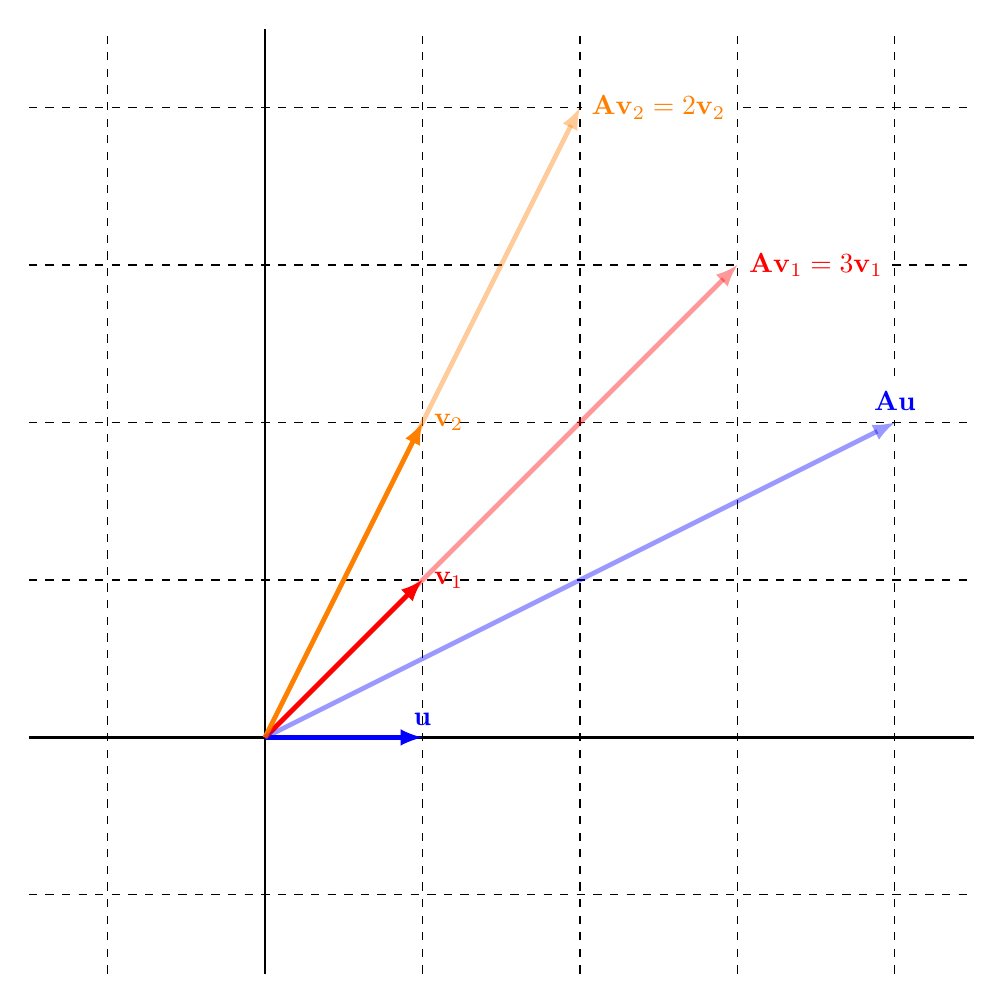
\begin{tikzpicture}
  \draw[thick] (-3,0) -- (9,0);
  \draw[thick] (0,-3) -- (0,9);
  \foreach \x in {-2,0,2,4,6,8}
    \draw[dashed] (\x,-3) -- (\x,9);
  \foreach \y in {-2,-2,0,2,4,6,8}
    \draw[dashed] (-3,\y) -- (9,\y);
  \draw[-latex,line width=0.6mm,color=blue]   (0,0) -- (2,0) node [above,color=blue]    {$\mathbf{u}$};
  \draw[-latex,line width=0.6mm,color=red]    (0,0) -- (2,2) node [right,color=red]     {$\mathbf{v}_1$};
  \draw[-latex,line width=0.6mm,color=orange] (0,0) -- (2,4) node [right,color=orange]  {$\mathbf{v}_2$};

  \draw[-latex,line width=0.6mm,color=blue,   opacity=0.4] (0,0) -- (8,4) node [above,color=blue,  opacity=1,fill=white] {$\mathbf{A u}$};
  \draw[-latex,line width=0.6mm,color=red,    opacity=0.4] (0,0) -- (6,6) node [right,color=red,   opacity=1,fill=white] {$\mathbf{Av}_1 = 3 \mathbf{v}_1$};
  \draw[-latex,line width=0.6mm,color=orange, opacity=0.4] (0,0) -- (4,8) node [right,color=orange,opacity=1,fill=white] {$\mathbf{Av}_2 = 2 \mathbf{v}_2$};
\end{tikzpicture}
\caption{Illustration of a the application of a matrix on a non-eigenvector $\mathbf{u}$ and an eigenvector $\mathbf{v}$.}
\label{Fig:linearAlgebra_illustrationEigenvectors}
\end{center}
\end{figure}

One thing to note is that eigenvectors are unique up to an arbitrary multiplicative scaling constant. So in the example, $[ 1/2 \ 1/2 ]^\top$ and $[ -3 \ -6 ]^\top$ are also eigenvectors. Also, many matrices we encounter in practical applications have entries that are real and symmetric or are Hermitian. In these cases, the eigenvalues are real and the eigenvectors are orthogonal, which can be then used to form an orthogonal basis. (As seen in the example, this is not true of a general matrix.)

Next, we will discuss computing the eigenvalues and eigenvectors using analytical techniques. Then, we will show how to decompose a matrix into a product of matrices containing the eigenvalues and eigenvectors. This decomposition permits numerous applications including the evaluation of a function of a matrix and the solution of differential equations. This section will briefly touch upon an iterative numerical method (there are unfortunately no direct methods like Gaussian elimination for computing eigenvalues) for computing a single dominant (largest in magnitude) eigenvalue and eigenvector pair. Numerical methods for computing the entire set of eigenvalues and eigenvectors are very complicated and involve multiple steps; these are therefore outside the scope of this text and left for a more advanced course on numerical linear algebra.


%%%%%%%%%%%%%%%%%%%%%%%%%%%%%%%%%%%%%%%%%%%%%%%%%%%%%%%%%%%%%%%%%%%%%%%%%%%%%%%%%%%%%%%%%%%%%%%
\subsection{Calculating Eigenvalues}

To compute the eigenvalues, we solve the system:
\begin{align}
  ( \mathbf{A} - \lambda \mathbf{I} ) \mathbf{x} = \mathbf{0}.
\end{align}
We know that for $\mathbf{x}$ to be non-zero, then the determinant of $\mathbf{A} - \lambda \mathbf{I}$ must be zero. Therefore, we compute:
\begin{align}
  \left| \begin{array}{c c c c c} 
    a_{1,1} - \lambda   & a_{1,2}   & \cdots & a_{1,N-1}   & a_{1,N}  \\
  	a_{2,1}   & a_{2,2} - \lambda   & \cdots & a_{2,N-1}   & a_{2,N}  \\
	\vdots    & \vdots    & \ddots  & \vdots      & \vdots   \\
	a_{N-1,1} & a_{N-1,2} & \cdots & a_{N-1,N-1} - \lambda & a_{N-1,N} \\ 
	a_{N,1}   & a_{N,2}   & \cdots & a_{N,N-1}   & a_{N,N}   - \lambda  \\ 
	\end{array} \right|  = 0. 
\end{align}
This yields, a polynomial up to degree $N$ in unknown $\lambda$, which has $N$ roots or eigenvalues. For $N > 4$, usually the roots $\lambda$ will have to be found numerically. (Rarely is numerical root finding used for large values of $N$, as there are more robust iterative methods available.)

An important special case is when $\mathbf{A}$ is a triangular matrix, which shows up frequently enough (e.g., in radioactive decay problems) to merit its own discussion. When $\mathbf{A}$ can be written in upper triangular form,
\begin{align}
  \left| \begin{array}{c c c c c} 
    a_{1,1} - \lambda   & 0   & \cdots & 0   & 0 \\
  	a_{2,1}   & a_{2,2} - \lambda   & \cdots & 0   & 0  \\
	\vdots    & \vdots    & \ddots  & \vdots      & \vdots   \\
	a_{N-1,1} & a_{N-1,2} & \cdots & a_{N-1,N-1} - \lambda & 0 \\ 
	a_{N,1}   & a_{N,2}   & \cdots & a_{N,N-1}   & a_{N,N}   - \lambda  \\ 
	\end{array} \right|  = 0, 
\end{align}
we can easily evaluate the determinant. As we decompose the matrix from an $N$$\times$$N$ determinant, to a $(N-1)$$\times$$(N-1)$, to a $(N-2)$$\times$$(N-2)$, and so on, we can observe that in all cases all but the first element of the first row are zero. This yields a product
\begin{align}
  \mathrm{det}(\mathbf{A} - \lambda \mathbf{I}) = ( a_{1,1} - \lambda ) ( a_{2,2} - \lambda ) \cdots ( a_{N,N} - \lambda ) = 0,
\end{align}
which means the roots $\lambda$ are the diagonal elements of the matrix. (As we will see, these corresponds to the radioactive decay constants.)

To show this in practice, let us do a few examples. 

%%%%%%%%%%%%%%%%%%%%%%%%%%%%%%%%%%%%%%%%%%%%%%%%%%%%%%%%%%%%%%%%%%%%%%%%%%%%%%%%%%%%%%%%%%%%%%%
\subsubsection{Example 1} 

First, consider the matrix
\begin{subequations}
\begin{align}
  \mathbf{A} =
  \left[ \begin{array}{c c c}
   5 &  4 & -2 \\
   4 &  5 &  2 \\
   0 &  2 & -2 \\ \end{array} \right] .
\end{align}
To find the eigenvectors of $\mathbf{A}$, we take the determinant of $\mathbf{A} - \lambda \mathbf{I} = 0$ and solve for $\lambda$:
\begin{align}
  \det{ \mathbf{A} - \lambda \mathbf{I} } &=
  \left| \begin{array}{c c c}
   5 - \lambda &            4 &           -2 \\
             4 &  5 - \lambda &            2 \\
             0 &            2 & -2 - \lambda \\ \end{array} \right| = 0, \nonumber \\
  &= ( 5 - \lambda) \left[ ( 5 - \lambda ) ( -2 - \lambda ) - 4 \right] \nonumber \\
  &- 4 \left[ 4 (-2 - \lambda) - 0 \right] \nonumber \\
  &+ (-2) \left( 8 - 0 \right) = 0, \nonumber \\
  &= \lambda^3 - 8 \lambda^2 - 15 \lambda + 54 = 0.
\end{align}
Solving for the roots $\lambda$ of this cubic polynomial gives the result:
\begin{align}
  \lambda = 9, 2, -3.
\end{align}
\end{subequations}

%%%%%%%%%%%%%%%%%%%%%%%%%%%%%%%%%%%%%%%%%%%%%%%%%%%%%%%%%%%%%%%%%%%%%%%%%%%%%%%%%%%%%%%%%%%%%%%
\subsubsection{Example 2} 

Next, consider the matrix
\begin{subequations}
\begin{align}
  \mathbf{A} =
  \left[ \begin{array}{c c c}
   3 & -1 &  2 \\
   3 & -1 &  6 \\
  -2 &  2 & -2 \\ \end{array} \right] .
\end{align}
To find the eigenvectors of $\mathbf{A}$, we again take the determinant of $\mathbf{A} - \lambda \mathbf{I} = 0$ and solve for $\lambda$:
\begin{align}
  \det{ \mathbf{A} - \lambda \mathbf{I} } &=
  \left| \begin{array}{c c c}
   3 - \lambda &           -1 &            2 \\
             3 & -1 - \lambda &            6 \\
            -2 &            2 & -2 - \lambda \\ \end{array} \right| = 0, \nonumber \\
  &= ( 3 - \lambda) \left[ ( -1 - \lambda ) ( -2 - \lambda ) - 12 \right] \nonumber \\
  &- (-1) \left[ 3 (-2 - \lambda) - (-12) \right] \nonumber \\
  &+ 2 \left[ 6 - (-2)( -1 - \lambda) \right] = 0, \nonumber \\
  &= \lambda^3 - 12 \lambda - 16 = 0.
\end{align}
Solving for the roots $\lambda$ gives:
\begin{align}
  \lambda = -4, 2, 2.
\end{align}
\end{subequations}
Note that here we have repeated eigenvalues.

%%%%%%%%%%%%%%%%%%%%%%%%%%%%%%%%%%%%%%%%%%%%%%%%%%%%%%%%%%%%%%%%%%%%%%%%%%%%%%%%%%%%%%%%%%%%%%%
\subsubsection{Example 3} 

Finally, consider a third matrix
\begin{subequations}
\begin{align}
  \mathbf{A} =
  \left[ \begin{array}{c c c}
   2 & -1 &  0 \\
   0 &  1 &  1 \\
  -1 &  1 &  2 \\ \end{array} \right] .
\end{align}
To find the eigenvectors of $\mathbf{A}$, we again take the determinant of $\mathbf{A} - \lambda \mathbf{I} = 0$ and solve for $\lambda$:
\begin{align}
  \det{ \mathbf{A} - \lambda \mathbf{I} } &=
  \left| \begin{array}{c c c}
   2 - \lambda &           -1 &            0 \\
             0 &  1 - \lambda &            1 \\
            -1 &            1 &  2 - \lambda \\ \end{array} \right| = 0, \nonumber \\
  &= ( 2 - \lambda) \left[ ( ( 1 - \lambda ) ( -2 - \lambda ) - 1 \right] + 1, \nonumber \\
  &= \lambda^3 - 5 \lambda^2 + 7 \lambda - 3 = 0.
\end{align}
Solving for the roots $\lambda$ gives:
\begin{align}
  \lambda = 3, 1, 1.
\end{align}
\end{subequations}
As with the previous example, this has a repeated root.

%%%%%%%%%%%%%%%%%%%%%%%%%%%%%%%%%%%%%%%%%%%%%%%%%%%%%%%%%%%%%%%%%%%%%%%%%%%%%%%%%%%%%%%%%%%%%%%
\subsection{Calculating Eigenvectors}

To find the eigenvectors, we solve the linear system
\begin{align}
  ( \mathbf{A} - \lambda \mathbf{I} ) \mathbf{x} = \mathbf{0}
\end{align}
for each value of $\lambda$. Since the determinant of the matrix $( \mathbf{A} - \lambda \mathbf{I} )$ is zero, the system does not have a unique solution and will have a rank that is less than the number of rows. All solutions may therefore be scaled by an arbitrary multiplicative constant. To illustrate the idea, let us revisit our examples. 

%%%%%%%%%%%%%%%%%%%%%%%%%%%%%%%%%%%%%%%%%%%%%%%%%%%%%%%%%%%%%%%%%%%%%%%%%%%%%%%%%%%%%%%%%%%%%%%
\subsubsection{Example 1} 

The first example matrix
\begin{subequations}
\begin{align}
  \mathbf{A} =
  \left[ \begin{array}{c c c}
   5 &  4 & -2 \\
   4 &  5 &  2 \\
   0 &  2 & -2 \\ \end{array} \right] .
\end{align}
has three eigenvalues: $\lambda_1 = 9, \lambda_2 = 2, \lambda_3 = -3$, which we index in descending order. Evaluating $( \mathbf{A} - \lambda \mathbf{I} )$ for $\lambda_1 = 9$ gives the matrix
\begin{align}
  \mathbf{A} - 9 \mathbf{I} =
  \left[ \begin{array}{c c c}
  -4 &  4 &  -2 \\
   4 & -4 &   2 \\
   0 &  2 & -11 \\ \end{array} \right] .
\end{align}
Now we use Gaussian elimination to put the matrix into a reduced-row echelon form. First, replace row $\circled{2}$ by the sum of rows $\circled{2}$ and $\circled{1}$:
\begin{align}
  \left[ \begin{array}{c c c}
  -4 &  4 &  -2 \\
   4 & -4 &   2 \\
   0 &  2 & -11 \\ \end{array} \right] 
   : \circled{2} \rightarrow \circled{2} + \circled{1} :
  \left[ \begin{array}{c c c}
  -4 &  4 &  -2 \\
   0 &  0 &   0 \\
   0 &  2 & -11 \\ \end{array} \right]   
\end{align}
Next, swap rows $\circled{2}$ and $\circled{3}$:
\begin{align}
  \left[ \begin{array}{c c c}
  -4 &  4 &  -2 \\
   0 &  0 &   0 \\
   0 &  2 & -11 \\ \end{array} \right]
   : \circled{2} \leftrightarrow \circled{3} :
  \left[ \begin{array}{c c c}
  -4 &  4 &  -2 \\
   0 &  2 & -11 \\
   0 &  0 &   0 \\  \end{array} \right] .
\end{align}
Now to eliminate the (1,2) element, replace row $\circled{1}$ with the difference of rows $\circled{1}$ and twice $\circled{2}$:
\begin{align}
  \left[ \begin{array}{c c c}
  -4 &  4 &  -2 \\
   0 &  2 & -11 \\
   0 &  0 &   0 \\  \end{array} \right] 
   : \circled{1} \rightarrow \circled{1} - 2 \times \circled{2}  :
  \left[ \begin{array}{c c c}
  -4 &  0 &  20 \\
   0 &  2 & -11 \\
   0 &  0 &   0 \\  \end{array} \right] .
\end{align}
Since we have a row of all zeros, we have one free parameter. Define 
\begin{align}
  x_3 = \alpha .
\end{align}
Then, using the second row:
\begin{align}
  2 x_2 - 11 \alpha &= 0, \nonumber \\
  x_2 &= \frac{11}{2} \alpha.
\end{align}
Finally, using the first row:
\begin{align}
 -4 x_1 + 20 \alpha &= 0, \nonumber \\
  x_1 &= 5 \alpha.
\end{align}
Writing out the solution vector:
\begin{align}
  \mathbf{x} = \alpha \left[ \begin{array}{c} 5 \\ \rfrac{11}{2} \\ 1 \\ \end{array} \right]
  \rightarrow \alpha \left[ \begin{array}{c} 10 \\ 11 \\ 2 \\ \end{array} \right] .
\end{align}
Since $\alpha$ is an arbitrary constant, we may redefine $\alpha$ to scale the results to get the solution vector in terms of whole numbers. This implies the eigenvector corresponding to $\lambda = 9$ is
\begin{align}
  \mathbf{v}_1 &= \left[ \begin{array}{c} 10 \\ 11 \\ 2 \\ \end{array} \right] .
\end{align}
Moving onto $\lambda_2 = 2$, the matrix
\begin{align}
  \mathbf{A} - 2 \mathbf{I} =
  \left[ \begin{array}{c c c}
   3 &  4 &  -2 \\
   4 &  3 &   2 \\
   0 &  2 &  -4 \\ \end{array} \right] .
\end{align}
After performing Gaussian elimination we obtain the matrix
\begin{align}
  \left[ \begin{array}{c c c}
   1 &  0 &  2 \\
   0 &  1 & -2 \\
   0 &  0 &  0 \\ \end{array} \right] .
\end{align}
As before, define
\begin{align}
  \alpha = x_3;
\end{align}
then,
\begin{align}
  x_2 - 2 \alpha &= 0, \nonumber \\
  x_2 &= 2 \alpha,
\end{align}
and
\begin{align}
  x_1 + 2 \alpha &= 0, \nonumber \\
  x_1 &= -2 \alpha.
\end{align}
Therefore, the solution vector is
\begin{align}
  \mathbf{x} = \alpha \left[ \begin{array}{c} -2 \\ 2 \\ 1 \\ \end{array} \right] 
\end{align}
and the eigenvector corresponding to $\lambda_2 = 2$ is
\begin{align}
  \mathbf{v}_2 = \left[ \begin{array}{c} -2 \\ 2 \\ 1 \\ \end{array} \right] .
\end{align}
Repeating the same procedure for $\lambda = -3$, we find the corresponding eigenvector
\begin{align}
  \mathbf{v}_3 = \left[ \begin{array}{c}  1 \\ -1 \\ 2 \\ \end{array} \right] .
\end{align}
\end{subequations}

%%%%%%%%%%%%%%%%%%%%%%%%%%%%%%%%%%%%%%%%%%%%%%%%%%%%%%%%%%%%%%%%%%%%%%%%%%%%%%%%%%%%%%%%%%%%%%%
\subsubsection{Example 2} 

For the second example, recall the matrix
\begin{subequations}
\begin{align}
  \mathbf{A} =
  \left[ \begin{array}{c c c}
   3 & -1 &  2 \\
   3 & -1 &  6 \\
  -2 &  2 & -2 \\ \end{array} \right] 
\end{align}
has eigenvalues $\lambda_1 = -4, \lambda_2 = 2, \lambda_3 = 2$ with one of these repeated. For $\lambda_1 = -4$, the process is identical to the previous example and we obtain the eigenvector
\begin{align}
  \mathbf{v}_1 = \left[ \begin{array}{c} -1 \\ -3 \\ 2 \\ \end{array} \right] .
\end{align}
For the $\lambda_2 = \lambda_3 = 2$ eigenvector, we obtain the matrix
\begin{align}
  \mathbf{A} - 2 \mathbf{I} =
  \left[ \begin{array}{c c c}
   1 & -1 &  2 \\
   3 & -3 &  6 \\
  -2 &  2 & -4 \\ \end{array} \right] .
\end{align}
We proceed with Gaussian elimination to obtain
\begin{align}
  \left[ \begin{array}{c c c}
   1 & -1 &  2 \\
   0 &  0 &  0 \\
   0 &  0 &  0 \\ \end{array} \right] .
\end{align}
Since we have a single nonzero row, the rank is 1 and we have 3 - 1 = 2 free parameters. Define
\begin{align}
  \alpha &= x_2, \\
  \beta &= x_3. 
\end{align}
Then,
\begin{align}
  x_1 = \alpha - 2 \beta .
\end{align}
This results in the solution vector
\begin{align}
  \mathbf{x} = 
  \alpha \left[ \begin{array}{c}  1 \\ 1 \\ 0 \\ \end{array} \right] +
  \beta  \left[ \begin{array}{c} -2 \\ 0 \\ 1 \\ \end{array} \right] .
\end{align}
Each of these column vectors corresponds to an eigenvector, so therefore
\begin{align}
  \mathbf{v}_2 &=  \left[ \begin{array}{c}  1 \\ 1 \\ 0 \\ \end{array} \right], \\
  \mathbf{v}_3 &=  \left[ \begin{array}{c} -2 \\ 0 \\ 1 \\ \end{array} \right].
\end{align}
\end{subequations}

%%%%%%%%%%%%%%%%%%%%%%%%%%%%%%%%%%%%%%%%%%%%%%%%%%%%%%%%%%%%%%%%%%%%%%%%%%%%%%%%%%%%%%%%%%%%%%%
\subsubsection{Example 3} 

Continuing to the third example, the matrix
\begin{subequations}
\begin{align}
  \mathbf{A} =
  \left[ \begin{array}{c c c}
   2 & -1 &  0 \\
   0 &  1 &  1 \\
  -1 &  1 &  2 \\ \end{array} \right] 
\end{align}
has eigenvalues $\lambda_1 = 3, \lambda_2 = 1, \lambda_3 = 1$. The eigenvector for $\lambda_1 = 3$ is
\begin{align}
  \mathbf{v}_1 &=  \left[ \begin{array}{c}  -1 \\ 1 \\ 2 \\ \end{array} \right] .
\end{align}
For the eigenvector $\lambda_2 = \lambda_3 = 1$, we obtain the following matrix in reduced-row echelon form:
\begin{align}
  \left[ \begin{array}{c c c}
   1 & -1 &  0 \\
   0 &  0 &  1 \\
   0 &  0 &  0 \\ \end{array} \right] .
\end{align}
From this, we know there will be one free nonzero parameter. However,
\begin{align}
  x_3 = 0, \\
  x_1 = x_2.
\end{align}
Since $x_3$ is uniquely determined at zero, we cannot assign the free parameter to it, so we are left with assigning the free parameter to one of the others. This implies the solution vector is
\begin{align}
  \mathbf{x} = \alpha \left[ \begin{array}{c}  1 \\ 1 \\ 0 \\ \end{array} \right] .
\end{align}
Therefore, we have only one linearly independent eigenvector corresponding to the repeated eigenvalue 1, which is
\begin{align}
  \mathbf{v}_2 =  \left[ \begin{array}{c}  1 \\ 1 \\ 0 \\ \end{array} \right] .
\end{align}

The upshot shown by these three examples is that if we have $N$ distinct eigenvalues, we will have $N$ distinct eigenvectors. If we have $N$ eigenvalues with some of them repeating, we may have $N$ distinct eigenvectors, but we could have fewer.

\end{subequations}

%%%%%%%%%%%%%%%%%%%%%%%%%%%%%%%%%%%%%%%%%%%%%%%%%%%%%%%%%%%%%%%%%%%%%%%%%%%%%%%%%%%%%%%%%%%%%%%
\subsection{Example: Nuclear Criticality}

The criticality of a nuclear system describes its ability to sustain a nuclear chain reaction. The criticality is described by the effective multiplication factor, which is an eigenvalue. The corresponding eigenvector (or eigenfunction) describes the neutron distribution throughout the system. Analysis or nuclear reactors depends upon being able to determine the criticality of a system. Furthermore, even outside the context of nuclear reactors, many industrial processes in the nuclear industry involve fissile materials and it is crucial to the safety of personnel that these processes never be in a configuration that would lead to a self sustaining chain reaction.

A simplified model of a nuclear system will treat it as an infinite homogeneous system (not a terrible first cut at analyzing a large reactor) where the dependent variable is the distribution of neutron kinetic energy $\phi(E)$ or the energy spectrum. The equation has the following form:
\begin{align}
  \sigma_t(E) \phi(E) - \int_0^\infty \sigma_s(E' \rightarrow E) \phi(E') dE' = \frac{\chi(E)}{k} \int_0^\infty \nu \sigma_f(E') \phi(E') dE'.
\end{align}
The first term on the left-hand side in the equation is the total collision rate of neutrons, the second term on the left-hand side describes the scattering process that leads to neutrons slowing down and thermalizing, and the term on the right-hand side describes the emission of fission neutrons. Note that the fission term has a factor of $\frac{1}{k}$, which describes the criticality of the system with $k$ being the effective multiplication factor. 

This equation is an integral equation (similar to a differential equation) and is difficult to solve except in the most simple conditions. As is the case when encountering a problem that is too difficult to solve, we develop an approximate form. This form is obtained by assuming the neutron kinetic energies can be described by a series of discrete \emph{energy groups}. We can do through a series of manipulations (you will see this in a reactor physics course) to obtain an approximate linear system for a group $g$:
\begin{align}
  \sigma_{tg} \phi_g - \sum_{g'=1}^G \sigma_{sg,g'} \phi_{g'} = \frac{\chi_g}{k} \sum_{g'=1}^G \nu \sigma_{fg'} \phi_{g'}.
\end{align}
Here: $\phi_g$ is the unknown neutron scalar flux (path-length density) in energy group $g$, $\sigma_{tg}$ is the cross section for total neutron interactions in group $g$, $\sigma_{sg,g'}$ is the rate that neutrons scatter from group $g'$ into group $g$, $\chi_g$ is the probability that a fission neutron is born in group $g$, and $\sigma_{fg}$ is the neutron fission production cross section in group $g$.

We can put this in matrix vector form by defining the neutron net removal matrix:
\begin{align}
  \mathbf{T} = \left[ \begin{array}{r r r r r r}
  \sigma_{t1} - \sigma_{s1,1} &             - \sigma_{s1,2} &   -\sigma_{s1,3} & \cdots &              -\sigma_{s1,G-1}   &              - \sigma_{s1,G} \\ 
               -\sigma_{s2,1} & \sigma_{t2} - \sigma_{s2,2} &   -\sigma_{s2,3} & \cdots &              -\sigma_{s2,G-1}   &              - \sigma_{s2,G} \\ 
                       \ldots &                      \ldots &           \ldots & \ddots &                        \ldots   &                       \ldots \\ 
             -\sigma_{sG-1,1} &             \sigma_{sG-1,2} & -\sigma_{sG-1,3} & \cdots & \sigma_{tG-1}-\sigma_{sG-1,G-1} &            - \sigma_{sG-1,G} \\ 
               -\sigma_{sG,1} &               \sigma_{sG,2} &   -\sigma_{sG,3} & \cdots &              -\sigma_{sG,G-1}    & \sigma_{tG} - \sigma_{sG,G} \\ 
  \end{array} \right] ;
\end{align}
and the neutron production matrix as a product of a column and row vector:
\begin{align}
  \mathbf{F} &= 
  \left[ \begin{array}{c} \chi_1 \\ \chi_2 \\ \chi_3 \\ \vdots \\ \chi_{G-1} \\ \chi_G \\ \end{array} \right]
  \left[ \begin{array}{c c c c c c}
  \nu \sigma_{f1} & \nu \sigma_{f2} & \nu \sigma_{f3} & \cdots & \nu \sigma_{fG-1} & \nu \sigma_{fG} \\ \end{array} \right] .
\end{align}
In matrix-vector form, this equation is then
\begin{align}
  \mathbf{T} \boldsymbol\phi = \frac{1}{k} \mathbf{F} \boldsymbol\phi
\end{align}
where $\boldsymbol\phi$ is a column vector of group neutron scalar fluxes.

It is often the case that $\mathbf{F}$ is non-invertable because $\chi_g \approx 0$ for low energy groups. Therefore, we can recast this problem as
\begin{align}
  k \boldsymbol\phi =  \mathbf{T}^{-1} \mathbf{F} \boldsymbol\phi .
\end{align}
Since $\mathbf{T}^{-1} \mathbf{F}$ is an operator, this is an eigenvalue problem. This is often written in terms of the fission source where we define
\begin{align}
  \mathbf{f} = \mathbf{F} \boldsymbol\phi,
\end{align}
which gives the rate that fission neutrons are born for each energy group. Multiplying the neutron balance equation by $\mathbf{F}$ we can obtain the form
\begin{align}
   \mathbf{F} \mathbf{T}^{-1} \mathbf{f} = k \mathbf{f}.
\end{align}
The operator $\mathbf{F} \mathbf{T}^{-1}$ has a physical significance. The meaning of $\mathbf{T}^{-1}$ is to transport neutrons from a source through the lifetime while treating fission as a loss (since the net removal operator does not involve fission). The meaning of $\mathbf{F} \mathbf{T}^{-1}$ is to transport neutrons from a source through a single fission generation. Therefore, the equation can be viewed as taking neutrons from a fission source, transporting them through one fission generation to form a new fission source, with $k$ being a scaling factor on the magnitude of that source. This gives an interpretation of $k$ as the number of neutrons in a fission generation divided by the number of neutrons in the previous fission generation.


%%%%%%%%%%%%%%%%%%%%%%%%%%%%%%%%%%%%%%%%%%%%%%%%%%%%%%%%%%%%%%%%%%%%%%%%%%%%%%%%%%%%%%%%%%%%%%%
\subsection{Matrix Eigendecomposition}

One of the most important applications of eigenvalues and eigenvectors is that many matrices can be expressed in terms of them. One example that we will encounter in the next chapter is in the solution of systems of linear ordinary differential equations. If an $N \times N$ matrix has $N$ linearly independent eigenvectors, then we say the matrix is \emph{diagonalizable} and can be written as
\begin{align}
  \mathbf{A} = \mathbf{V D V}^{-1} .
\end{align}
Here $\mathbf{D}$ is a diagonal matrix containing the eigenvalues,
\begin{align}
  \mathbf{D} = \left[ \begin{array}{c c c c c}
  \lambda_1		& 0				& \cdots	& 0				& 0				\\
  0				& \lambda_2		& \cdots	& 0 			& 0				\\
  \vdots		& \vdots		& \ddots	& \vdots		& \vdots		\\
  0				& 0				& \cdots	& \lambda_{N-1}	& 0				\\
  0				& 0				& \cdots	& 0				& \lambda_{N} 	\\ \end{array} \right] ,
\end{align}
and $\mathbf{V}$ is a matrix where its columns are the corresponding eigenvectors,
\begin{align}
  \mathbf{V} = \left[ \begin{array}{c c c c c}
  				&				&			&					&					\\
  \mathbf{v}_1	& \mathbf{v}_1	& \cdots	& \mathbf{v}_{N-1}	& \mathbf{v}_N		\\
  				&				&			&					&					\\ \end{array} \right] .
\end{align}
The ordering is arbitrary, but conventionally, the matrices are ordered such that $|\lambda_1| \ge |\lambda_2| \ge \cdots \ge |\lambda_N|$.

Most matrices encountered in science and engineering applications are diagonalizable. Occasionally, there are cases where a matrix does not have $N$ linearly independent eigenvectors. These matrices are called \emph{defective matrices}. It is possible to generalize the eigendecompositon in this case. The matrix $\mathbf{V}$ has the eigenvectors as columns plus additional vectors using something called the Jordan Normal Form. This is not encountered often, so is not discussed further here.
%For an eigenvector $\mathbf{v}_i$ with a repeated eigenvalue $\lambda_i$ with multiplicity $n$ with $k$ linearly independent eigenvalues, the remaining $n - k$ vectors can be obtained from the equation $( \mathbf{A} - \lambda \mathbf{I} ) \mathbf{v}_{i+1} = \mathbf{v}_i .
%\begin{align}
%  ( \mathbf{A} - \lambda \mathbf{I} ) \mathbf{v}_{k+i} = \mathbf{v}_{k+i-1}, \quad i = 1, \ldots , n - k.
%\end{align}

Revisiting our example, the matrix
\begin{align}
  \mathbf{A} =
  \left[ \begin{array}{c c c}
   5 &  4 & -2 \\
   4 &  5 &  2 \\
   0 &  2 & -2 \\ \end{array} \right]  \nonumber
\end{align}
has three unique eigenvalues $\lambda = 9, -3, 2$. Note the conventional ordering from largest to smallest magnitude. The eigendecomposition has the following matrices:
\begin{align}
  \mathbf{D} =  \left[ \begin{array}{c c c}
  9				& 0				& 0			\\
  0				& -3			& 0			\\
  0				& 0				& 2			\\ \end{array} \right] , \quad
 \mathbf{V} =  \left[ \begin{array}{c c c}
  10			& -2			&  1			\\
  11			&  2			& -1			\\
  2				&  1			&  2			\\ \end{array} \right]  . \nonumber
\end{align}
In the second example, 
\begin{align}
  \mathbf{A} =
  \left[ \begin{array}{c c c}
   3 & -1 &  2 \\
   3 & -1 &  6 \\
  -2 &  2 & -2 \\ \end{array} \right] \nonumber
\end{align}
the eigenvalues are $\lambda = -4, 2, 2.$ We have a repeated eigenvalue, but there are still three linearly independent eigenvectors. Therefore this matrix is diagonalizable:
\begin{align}
  \mathbf{D} =  \left[ \begin{array}{c c c}
 -4				& 0				& 0			\\
  0				& 2				& 0			\\
  0				& 0				& 2			\\ \end{array} \right] , \quad
 \mathbf{V} =  \left[ \begin{array}{c c c}
  -1			&  1			& -2			\\
   2			&  1			&  0			\\
   3			&  0			&  1			\\ \end{array} \right]  . \nonumber
\end{align}
For the third example, 
\begin{align}
  \mathbf{A} =
  \left[ \begin{array}{c c c}
   2 & -1 &  0 \\
   0 &  1 &  1 \\
  -1 &  1 &  2 \\ \end{array} \right] , \nonumber
\end{align}
there is only two linearly independent eigenvectors. This means this matrix is defective and not diagonalizable.

%%%%%%%%%%%%%%%%%%%%%%%%%%%%%%%%%%%%%%%%%%%%%%%%%%%%%%%%%%%%%%%%%%%%%%%%%%%%%%%%%%%%%%%%%%%%%%%
\subsection{Functions of Matrices}

One important application of the eigendecomposition is taking a function of a matrix $f(\mathbf{A})$. This arises, for example, when solving systems of ordinary linear differential equations. We can evaluate the function of any diagonalizable matrix provided that the function is analytic, in that it has a power series expansion:
\begin{align}
  f(\mathbf{A}) = c_0 + c_1 \mathbf{A} + c_2 \mathbf{A}^2 + \ldots = \sum_{n=0}^\infty c_n \mathbf{A}^n .
\end{align}
If $\mathbf{A}$ is diagonalizable, then we can expand it as an eigendecomposition:
\begin{align}
  f(\mathbf{A}) = \sum_{n=0}^\infty c_n \left( \mathbf{V} \mathbf{D} \mathbf{V}^{-1} \right)^n .
\end{align}
Next, for an arbitrary power $n$, we note
\begin{align}
  \mathbf{A}^n &= \left( \mathbf{V} \mathbf{D} \mathbf{V}^{-1} \right)^n =  
  \left( \mathbf{V} \mathbf{D} \mathbf{V}^{-1} \right) \left( \mathbf{V} \mathbf{D} \mathbf{V}^{-1} \right) \cdots \left( \mathbf{V} \mathbf{D} \mathbf{V}^{-1} \right) \left( \mathbf{V} \mathbf{D} \mathbf{V}^{-1} \right) \nonumber \\
  &= \mathbf{V} \mathbf{D} \mathbf{D} \cdots \mathbf{D} \mathbf{D} \mathbf{V}^{-1} = \mathbf{V} \mathbf{D}^n \mathbf{V}^{-1} .
\end{align}
Notice that for internal term has an adjacent $\mathbf{V}$ and $\mathbf{V}^{-1}$ so they all cancel, leaving only a single term on the end. Returning to the power series expansion:
\begin{align}
  f(\mathbf{A}) = \sum_{n=0}^\infty c_n \mathbf{V} \mathbf{D}^n \mathbf{V}^{-1} 
  = \mathbf{V} \left( \sum_{n=0}^\infty c_n \mathbf{D}^n \right) \mathbf{V}^{-1} =  \mathbf{V} f( \mathbf{D} ) \mathbf{V}^{-1}.
\end{align}
This means we need to evaluate the function of a diagonal matrix. Using the definition of a power series and noting that the sums and products of diagonal matrices are just diagonal matrices (they function as effectively independent variables), we have
\begin{align}
  \sum_{n=0}^\infty c_n \mathbf{D}^n &= 
  c_0 \mathbf{I} +
  c_1 \left[ \begin{array}{c c c}
  \lambda_1		& 0				& \cdots	\\
  0				& \lambda_2		& \cdots	\\
  \vdots		& \vdots		& \ddots	\\ \end{array} \right] +  
  c_2  \left[ \begin{array}{c c c}
  \lambda_1		& 0				& \cdots	\\
  0				& \lambda_2		& \cdots	\\
  \vdots		& \vdots		& \ddots	\\ \end{array} \right]^2 + \cdots \nonumber \\
  &= c_0 \mathbf{I} +
  c_1 \left[ \begin{array}{c c c}
  \lambda_1		& 0				& \cdots	\\
  0				& \lambda_2		& \cdots	\\
  \vdots		& \vdots		& \ddots	\\ \end{array} \right] +  
  c_2  \left[ \begin{array}{c c c}
  \lambda_1^2	& 0			& \cdots	\\
  0				& \lambda_2^2	& \cdots	\\
  \vdots		& \vdots		& \ddots	\\ \end{array} \right] + \cdots \nonumber \\
  &= \left[ \begin{array}{c c c}
  \displaystyle\sum_{n=0}^\infty c_n \lambda_1^n		& 0				& \cdots \vspace{0.2em}	\\
  0				& \displaystyle\sum_{n=0}^\infty c_n \lambda_2^n		& \cdots \vspace{0.2em}	\\
  \vdots		& \vdots		& \ddots	\\ \end{array} \right] 
  = \left[ \begin{array}{c c c}
  f(\lambda_1)		& 0			& \cdots 	\\
  0				& f(\lambda_2) 	& \cdots 	\\
  \vdots		& \vdots		& \ddots	\\ \end{array} \right] .
\end{align}
Therefore, the procedure for taking $f(\mathbf{A})$ is to first find the eigenvalues and eigenvectors of $\mathbf{A}$. The matrices $\mathbf{V}$ and $\mathbf{V}^{-1}$ are computed as before. The matrix $f(\mathbf{D})$ is a diagonal matrix where all of the elements are the function evaluations of the eigenvalues. 

Perhaps the most important example is matrix exponential, which arises in the solution of systems of linear ordinary differential equations. We have
\begin{align}
  \exp ( \mathbf{A} ) =  \mathbf{V} \exp ( \mathbf{D} ) \mathbf{V}^{-1} ,
\end{align}
where $\mathbf{D}$ contains the exponentials of the eigenvalues of $\mathbf{A}$. It is important to keep in mind that the matrix exponential is \emph{not} in general the exponential of the individual elements (diagonal matrices excepted). Rather, one needs to apply the eigendecomposition first.


%%%%%%%%%%%%%%%%%%%%%%%%%%%%%%%%%%%%%%%%%%%%%%%%%%%%%%%%%%%%%%%%%%%%%%%%%%%%%%%%%%%%%%%%%%%%%%%
\subsection{Power Iteration}

Solving for all of the eigenvalues and eigenvectors for a given matrix $\mathbf{A}$ on a computer is a complicated algorithmic task involving numerous steps. 

In many applications, we are primarily interested in the fundamental or largest (in magnitude) eigenvalue and its corresponding eigenvector, which we refer to as the dominant eigenpair. This eigenpair gives information about the long-time or asymptotic behavior of a particular system. In nuclear reactor analysis, the dominant eigenvalue is $k$, the effective multiplication factor and the corresponding eigenvector has information about the steady-state distribution of neutrons during continuous operation. Fortunately, there is an iterative algorithm that is fairly simple and can be used for obtaining this called the \emph{Power Iteration Method}. 

The general idea is that we make an initial guess of the eigenvector and make successive matrix multiplications of the matrix $\mathbf{A}$ upon it. Eventually, the resulting vector should, under certain circumstances, converge. The power iteration method is guaranteed to converge if the dominant eigenvalue is unique and all of the eigenvalues are real and positive, such as when $\mathbf{A}$ is a real-symmetric matrix. (In practice, this works extremely well for the application of nuclear criticality even though this has not rigorously been proven.) Problems with convergence may arise when eigenvalues are complex or when the second-largest eigenvalue is equal to or close to the largest.

The power iteration starts with a nonzero initial guess for a normalized eigenvector $\mathbf{v}^{(0)}$, and finds an updated guess by
\begin{align}
  \mathbf{u}^{(k)} &= \mathbf{A} \mathbf{v}^{(k-1)} , \\*
  \mathbf{v}^{(k)} &= \frac{ \mathbf{u}^{(k)} }{ | \mathbf{u}^{(k)} | } .
\end{align}
Here the superscript $k$ in parentheses is an iteration index. Note that the eigenvector needs to be normalized every iteration, else the magnitude of the eigenvector will grow without bound or decay to zero (unless the fundamental eigenvalue is 1).

The eigenvalue for the $k$th iteration is computed using something called the Rayleigh quotient. This can be derived by taking the dot product of $\mathbf{v}^{(k)}$ with the equation $\mathbf{A v}^{(k)} = \lambda^{(k)} \mathbf{v}^{(k)}$ and solving for $\lambda$:
\begin{align}
  \lambda^{(k)} = \frac{ ( \mathbf{A} \mathbf{v}^{(k)} ) \cdot \mathbf{v}^{(k)} }{ \mathbf{v}^{(k)} \cdot  \mathbf{v}^{(k)} } .
\end{align}
We then check the following convergence criterion:
\begin{align}
  | \mathbf{A} \mathbf{v}^{(k)} - \lambda^{(k)} \mathbf{v}^{(k)} | < \epsilon ,
\end{align}
where $\epsilon$ is a user-defined tolerance. If it is not met, we iterate again and again until the equation is satisfied to the specified tolerance; however, care needs to be taken to restrict the maximum number of iterations because there are situations (e.g., complex eigenvalues) where the algorithm will never converge. 

The power iteration method is quite robust for most linear systems that arise from approximating differential equations found in scientific and engineering applications. The primary issue with the method in practical applications is that it may exhibit slow convergence. Assuming the eigenvectors form an orthogonal basis that completely spans the space, the initial guess can be expanded as a linear combination of eigenvectors:
\begin{align}
  \mathbf{v}^{(0)} = c_1 \mathbf{v}_1 + c_2 \mathbf{v}_2 + \ldots + c_N \mathbf{v}_N .
\end{align}
Here the subscripts denote the eigenvectors $\mathbf{v}_i$ corresponding to the eigenvalues $\lambda_i$ such that $| \lambda_1 | \ge | \lambda_2 | \ge \cdots \ge | \lambda_N |$. To get the $k$th iterate of the eigenvector, we apply multiply the initial guess by the matrix $\mathbf{A}$ $k$ times:
\begin{align}
  \mathbf{v}^{(k)} = \mathbf{A}^k \mathbf{v}^{(0)} = c_1 \mathbf{A}^k \mathbf{v}_1 + c_2 \mathbf{A}^k \mathbf{v}_2 + \ldots + c_N \mathbf{A}^k \mathbf{v}_N .
\end{align}
Here $\mathbf{A}^k$ is the matrix to the $k$th power. Noting that the $\mathbf{v}_k$ are eigenvectors upon which $\mathbf{A}$ is being applied, we can then write:
\begin{align}
  \mathbf{v}^{(k)} = c_1 \lambda_1^k \mathbf{v}_1 + c_2 \lambda_2^k \mathbf{v}_2 + \ldots + c_N \lambda_1^N \mathbf{v}_N .
\end{align}
Factoring out $c_1 \lambda_1^k$ gives
\begin{align}
  \mathbf{v}^{(k)} = c_1 \lambda_1^k \left[ \mathbf{v}_1 + \frac{c_2}{c_1} \left( \frac{\lambda_2}{\lambda_1} \right)^k \mathbf{v}_2 + \frac{c_3}{c_1} \left( \frac{\lambda_3}{\lambda_1} \right)^k \mathbf{v}_3 + \ldots + \frac{c_N}{c_1} \left( \frac{\lambda_N}{\lambda_1} \right)^k\mathbf{v}_N \right].
\end{align}
By the ordering of the eigenvalues, the ratio of the eigenvalues is less then one in magnitude and $\lambda_2 / \lambda_1$ is the largest (in magnitude). This means when taken to the $k$th power, the $\lambda_2 / \lambda_1$ decays slower than the others. Therefore, the asymptotic rate of convergence is described the ratio of the second largest (in magnitude) eigenvalue to the largest:
\begin{align}
  \rho = \left| \frac{\lambda_2}{\lambda_1} \right| ,
\end{align}
sometimes referred to as the dominance ratio in the nuclear criticality discipline. When $\rho \approx 1$, this implies that the convergence rate is slow. In the application of nuclear reactor analysis, this is fairly typical of large, commercial reactors. Therefore, more advanced methods are used to accelerate convergence, but these are beyond the scope of this text.

To illustrate the power iteration method, let us revisit one of our examples:
\begin{align}
  \mathbf{A} =
  \left[ \begin{array}{c c c}
   5 &  4 & -2 \\
   4 &  5 &  2 \\
   0 &  2 & -2 \\ \end{array} \right] , \nonumber
\end{align}
where we found that the dominant eigenvalue and (normalized) eigenvector are
\begin{align}
  \lambda_1 = 9, \quad \mathbf{v}_1 = \frac{1}{15} \left[ \begin{array}{c} 10 \\ 11 \\ 2 \\ \end{array} \right] 
  \approx  \left[ \begin{array}{c} 0.66667 \\ 0.73333 \\ 0.13333 \\ \end{array} \right]. \nonumber
\end{align}
Let us guess the eigenvector
\begin{align}
  \mathbf{v}^{(0)} = \left[ \begin{array}{c} 1 \\ 1 \\ 1 \\ \end{array} \right] \nonumber
\end{align}
The first application of $\mathbf{A}$ gives the vectors
\begin{align}
  \mathbf{u}^{(1)} =   \left[ \begin{array}{c c c}
   5 &  4 & -2 \\
   4 &  5 &  2 \\
   0 &  2 & -2 \\ \end{array} \right]
   \left[ \begin{array}{c} 1 \\ 1 \\ 1 \\ \end{array} \right] =
   \left[ \begin{array}{c} 11 \\ 11 \\ 0 \\ \end{array} \right] , \quad
   \mathbf{v}^{(1)} =  \frac{\mathbf{u}^{(1)}}{| \mathbf{u}^{(1)} |} \approx \left[ \begin{array}{c} 0.536875  \\ 0.843661  \\ 0 \\ \end{array} \right] . \nonumber
\end{align}
The predicted eigenvalue is
\begin{align}
  \lambda^{(1)} = \frac{ ( \mathbf{A} \mathbf{v}^{(1)} ) \cdot \mathbf{v}^{(1)} }{ \mathbf{v}^{(1)} \cdot  \mathbf{v}^{(1)} } \approx 8.62353 . \nonumber
\end{align}
The error estimate on the equation is
\begin{align}
  | \mathbf{A} \mathbf{v}^{(1)} -  \lambda^{(1)} \mathbf{v}^{(1)} | \approx 2.39104. \nonumber
\end{align}
As expected the agreement with the equation is not good and the eigenvalue is still significantly different than the correct result of 9.

Multiplying $\mathbf{A}$ onto $\mathbf{v}^{(1)}$ and renormalizing gives
\begin{align}
  \mathbf{v}^{(2)} \approx
   \left[ \begin{array}{c} 0.677071  \\ 0.711353  \\ 0.188551 \\ \end{array} \right] , \quad \lambda^{(2)} \approx 8.88541 , \quad \text{Error $\approx$ } 0.725475 . \nonumber
\end{align}
Getting closer, but still not there. A few more iterations gives:
\begin{align}
  \mathbf{v}^{(3)} \approx
   &\left[ \begin{array}{c c c} 0.656610 & 0.745055 & 0.117286 \end{array} \right]^\top , \quad \lambda^{(3)} \approx 9.01291 , \quad \text{Error $\approx$ } 0.261228 . \nonumber \\
   \mathbf{v}^{(4)} \approx
   &\left[ \begin{array}{c c c} 0.668615 & 0.730455 & 0.139246 \end{array} \right]^\top , \quad \lambda^{(4)} \approx 8.99207 , \quad \text{Error $\approx$ } 0.082992 . \nonumber \\
   \mathbf{v}^{(5)} \approx
   &\left[ \begin{array}{c c c} 0.665714 & 0.734530 & 0.131490 \end{array} \right]^\top , \quad \lambda^{(5)} \approx 9.00214 , \quad \text{Error $\approx$ } 0.028480 . \nonumber \\
   \mathbf{v}^{(6)} \approx
   &\left[ \begin{array}{c c c} 0.666918 & 0.732988 & 0.133976 \end{array} \right]^\top , \quad \lambda^{(5)} \approx 8.99920 , \quad \text{Error $\approx$ } 0.009308 . 
\nonumber \\
   &\vdots \nonumber \\
    \mathbf{v}^{(10)} \approx
   &\left[ \begin{array}{c c c} 0.666670 & 0.733329 & 0.133341 \end{array} \right]^\top , \quad \lambda^{(10)} \approx 8.99999 , \quad \text{Error $\approx$ } 1.15591 \times 10^{-4} . \nonumber 
\end{align}
It appears that within ten iterations, the eigenvalue and eigenvector are fairly close and converging rapidly. Looking at the theoretical asymptotic convergence rate we have $\rho = \left| \frac{\lambda_2}{\lambda_1} \right| = \left| \frac{-3}{9} \right| = \frac{1}{3}$, which implies that the power iteration should quickly in this case.


%%%%%%%%%%%%%%%%%%%%%%%%%%%%%%%%%%%%%%%%%%%%%%%%%%%%%%%%%%%%%%%%%%%%%%%%%%%%%%%%%%%%%%%%%%%%%%%%
%%%%%%%%%%%%%%%%%%%%%%%%%%%%%%%%%%%%%%%%%%%%%%%%%%%%%%%%%%%%%%%%%%%%%%%%%%%%%%%%%%%%%%%%%%%%%%%%
\section{Singular Values}

Any matrix $\mathbf{A}$, even if it is not square, has a set of numbers called singular values, which are related to eigenvalues. Recall that the eigenvectors of a matrix give the directions that are invariant with respect to multiplication $\mathbf{A}$ up to a multiplicative scaling constant given by the corresponding eigenvalues. The singular vectors, on the other hand, give the directions of maximal action when multiplied by $\mathbf{A}$ where the respective singular values give a scaling constant. 

There has been a growing importance of singular values and the singular value decomposition (which is analogous to the eigendecomposition) over the last few decades, especially in the area of data science. One important application is finding the principal components, or the set of vectors that describe most of the information in a system. These singular vectors can be used to discern what quantities are most important for describing a system. They can also compactly approximate a matrix having information that describes a complicated system, allowing for data compression. In addition, we can use the singular value decomposition to compute a matrix called the pseudoinverse, which is a generalization of the normal inverse that exists for any matrix. This pseudoinverse can be used to solve optimization problems to find best fit for incomplete or even inconsistent data, which invariably arises in real-world measurements.

The equations that describe the singular values are
\begin{subequations}
\begin{align}
  \mathbf{A v} &= \sigma \mathbf{u}, \\
  \mathbf{A}^* \mathbf{u} &= \sigma \mathbf{v} .
\end{align}
\end{subequations}
Here $\mathbf{A}$ is any (even non square) matrix, $\sigma$ is a singular value, and $\mathbf{u}$ and $\mathbf{v}$ are respective left and right singular (unit) vectors, which are orthonormal. As with eigenvalues, there is a largest singular value $\sigma_1$. From this relationship, we can take the magnitude of the multiplicative action of $\mathbf{A}$ onto the corresponding right singular value $\mathbf{v}_1$ and get
\begin{align}
  | \mathbf{A v}_1 | = \sigma_1 .
\end{align}
The application of $\mathbf{A}$ onto $\mathbf{v}_1$ is the maximum possible stretching of any unit vector. In other words,
\begin{align}
  | \mathbf{A v}_1 | \ge | \mathbf{A x} | , \quad | \mathbf{x} | = 1 .
\end{align}

\begin{figure}[tb!]
\begin{center}
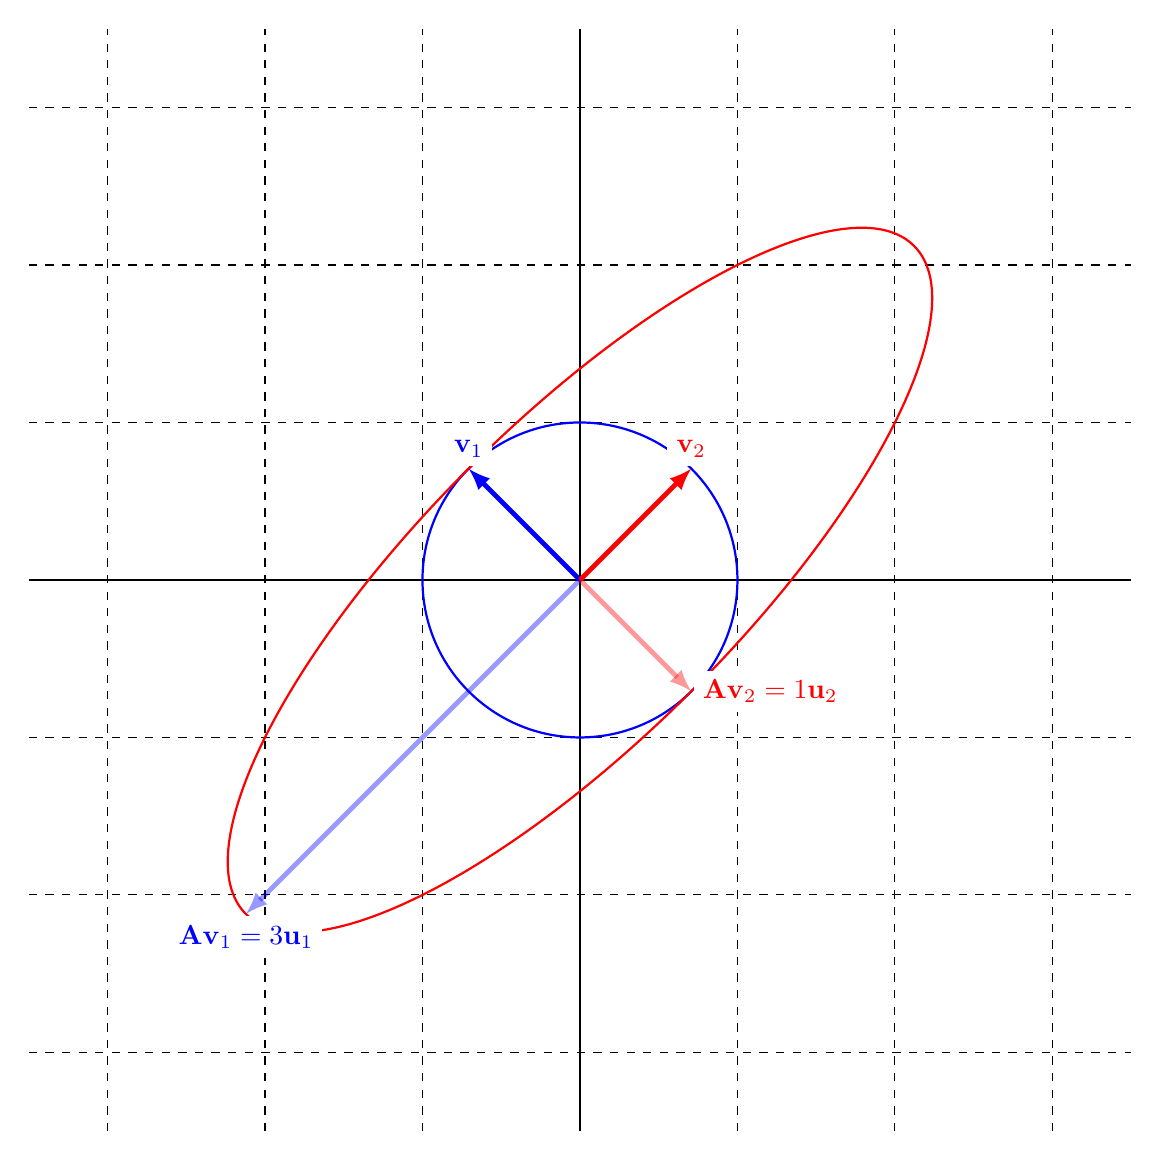
\begin{tikzpicture}
  \draw[thick] (-7,0) -- (7,0);
  \draw[thick] (0,-7) -- (0,7);
  \foreach \x in {-6,-4,-2,0,2,4,6}
    \draw[dashed] (\x,-7) -- (\x,7);
  \foreach \y in {-6,-4,-2,-2,0,2,4,6}
    \draw[dashed] (-7,\y) -- (7,\y);

  \draw[color=blue, thick]            (0,0) circle (2);
  \draw[color=red, rotate=45, thick]  (0,0) ellipse (6 and 2);

  \draw[-latex,line width=0.6mm,color=blue]    (0,0) -- (-1.414, 1.414) node [above,color=blue, fill=white] {$\mathbf{v}_1$};
  \draw[-latex,line width=0.6mm,color=red]     (0,0) -- ( 1.414, 1.414) node [above,color=red,  fill=white]  {$\mathbf{v}_2$};

  \draw[-latex,line width=0.6mm,color=blue,   opacity=0.4] (0,0) -- (-4.242,-4.242) node [below,color=blue,  opacity=1,fill=white] {$\mathbf{Av}_1 = 3 \mathbf{u}_1$};
  \draw[-latex,line width=0.6mm,color=red,    opacity=0.4] (0,0) -- ( 1.414,-1.414) node [right,color=red,   opacity=1,fill=white] {$\mathbf{Av}_2 = 1 \mathbf{u}_2$};


%  \draw[-latex,line width=0.6mm,color=orange, opacity=0.4] (0,0) -- (4,8) node [right,color=orange,opacity=1,fill=white] {$\mathbf{Av}_2 = 2 \mathbf{v}_2$};
\end{tikzpicture}
\caption{Illustration of a the application of a matrix on its right singular vectors.}
\label{Fig:linearAlgebra_illustrationSingularVectors}
\end{center}
\end{figure}

To illustrate this geometrically, let us consider the matrix
\begin{align}
  \mathbf{A} = \left[ \begin{array}{c c}
   2 & -1 \\
   1 & -2 \\ \end{array} \right] . \nonumber
\end{align}
Using techniques to be discussed, we will find that the singular values are $\sigma = 3, 1$; the corresponding right singular vectors are
\begin{align}
  \mathbf{v}_1 = \frac{1}{\sqrt{2}} \left[ \begin{array}{c} -1 \\ 1 \\ \end{array} \right] , \quad
  \mathbf{v}_2 = \frac{1}{\sqrt{2}} \left[ \begin{array}{c}  1 \\ 1 \\ \end{array} \right] ;
\end{align}
and the respective left singular vectors are
\begin{align}
  \mathbf{u}_1 = \frac{1}{\sqrt{2}} \left[ \begin{array}{c} -1 \\ -1 \\ \end{array} \right] , \quad
  \mathbf{u}_2 = \frac{1}{\sqrt{2}} \left[ \begin{array}{c}  1 \\ -1 \\ \end{array} \right] .
\end{align}
Observe that these two vectors within each set are orthonormal: their dot product $\mathbf{v}_1 \cdot \mathbf{v}_2 = 0$ and $\mathbf{u}_1 \cdot \mathbf{u}_2 = 0$  and their magnitudes are one. We can therefore draw the right singular values as two vectors on the unit circle. The application of $\mathbf{A}$ onto these vectors $\mathbf{v}$ yields the vectors $\mathbf{u}$ scaled by the respective singular values $\sigma$. These resulting vectors can now be thought of as the semi-axes of an ellipse. This is all illustrated in Fig.~\ref{Fig:linearAlgebra_illustrationSingularVectors}.

In general, the application of $\mathbf{A}$ maps its right singular vectors $\mathbf{v}$ from a $N$-dimensional sphere to an $M$-dimensional ellipsoid where $N \ge M$ with the left singular values $\mathbf{u}$ being the set of orthogonal directions of maximal stretching.

%%%%%%%%%%%%%%%%%%%%%%%%%%%%%%%%%%%%%%%%%%%%%%%%%%%%%%%%%%%%%%%%%%%%%%%%%%%%%%%%%%%%%%%%%%%%%%%
\subsection{Singular Value Decomposition} \label{Sec:linearAlgebra_singularValueDecomposition}

Any real $N$$\times$$M$ matrix $\mathbf{A}$ can be written as the product of three matrices using the singular value decomposition:
\begin{align} \label{Eqn:linearAlgebra_singularValueDecomposition}
  \mathbf{A} = \mathbf{U} \boldsymbol\Sigma \mathbf{V}^\top .
\end{align}
Here $\boldsymbol\Sigma$ is a $N$$\times$$M$ matrix where the diagonal elements $i = j$ contain the singular values with the remaining elements being zero, $\mathbf{V}$ is an $M$$\times$$M$ matrix containing the right singular values, and $\mathbf{U}$ is a $N$$\times$$N$ matrix containing the left singular values. An important property of $\mathbf{U}$ and $\mathbf{V}$ is that they are both unitary matrices, which means they equal their responses conjugate transposes (or just the transpose if all elements are real).

\begin{figure}[tb!]
\centering
\begin{subfigure}[b]{0.45\textwidth}
  \centering
  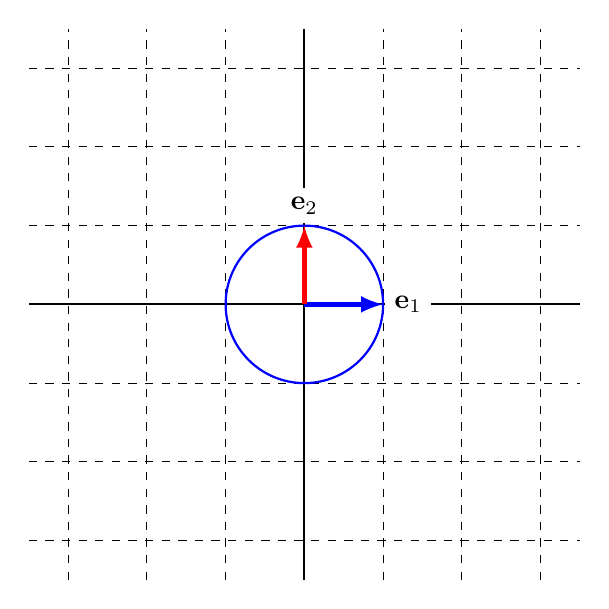
\begin{tikzpicture}
    \draw[thick] (-3.5,0) -- (3.5,0);
    \draw[thick] (0,-3.5) -- (0,3.5);
    \foreach \x in {-3,-2,-1,0,1,2,3}
      \draw[dashed] (\x,-3.5) -- (\x,3.5);
    \foreach \y in {-3,-2,-1,0,1,2,3}
      \draw[dashed] (-3.5,\y) -- (3.5,\y);

    \draw[color=blue, thick]            (0,0) circle (1);

    \draw[-latex,line width=0.6mm,color=blue]    (0,0) -- (1,0) node [right,color=black, fill=white]  {$\mathbf{e}_1$};
    \draw[-latex,line width=0.6mm,color=red]     (0,0) -- (0,1) node [above,color=black,  fill=white]  {$\mathbf{e}_2$};
  \end{tikzpicture}
  %\caption{$y=x$}
  %\label{fig:y equals x}
\end{subfigure}
\hfill
\begin{subfigure}[b]{0.45\textwidth}
  \centering
  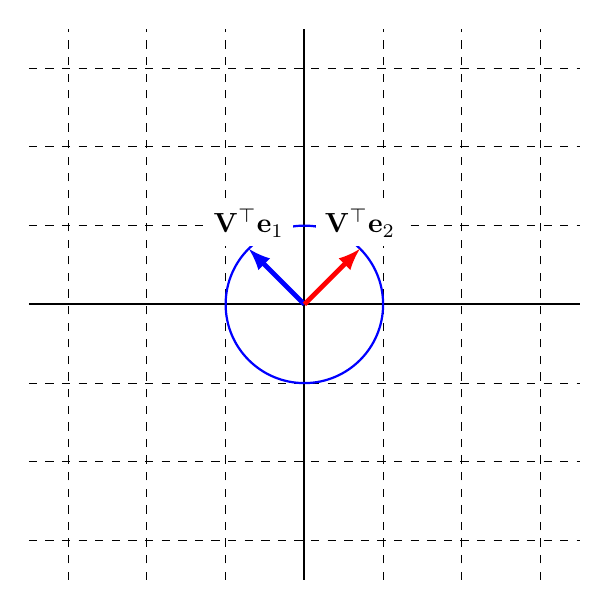
\begin{tikzpicture}
    \draw[thick] (-3.5,0) -- (3.5,0);
    \draw[thick] (0,-3.5) -- (0,3.5);
    \foreach \x in {-3,-2,-1,0,1,2,3}
      \draw[dashed] (\x,-3.5) -- (\x,3.5);
    \foreach \y in {-3,-2,-1,0,1,2,3}
      \draw[dashed] (-3.5,\y) -- (3.5,\y);

    \draw[color=blue, thick]            (0,0) circle (1);

    \draw[-latex,line width=0.6mm,color=blue]    (0,0) -- (-0.707, 0.707) node [above,color=black, fill=white]  {$\mathbf{V}^\top \mathbf{e}_1$};
    \draw[-latex,line width=0.6mm,color=red]     (0,0) -- ( 0.707, 0.707) node [above,color=black,  fill=white] {$\mathbf{V}^\top \mathbf{e}_2$};
  \end{tikzpicture}
  %\caption{$y=x$}
  %\label{fig:y equals x}
\end{subfigure}
\\ \vspace{1cm}
\begin{subfigure}[b]{0.45\textwidth}
  \centering
  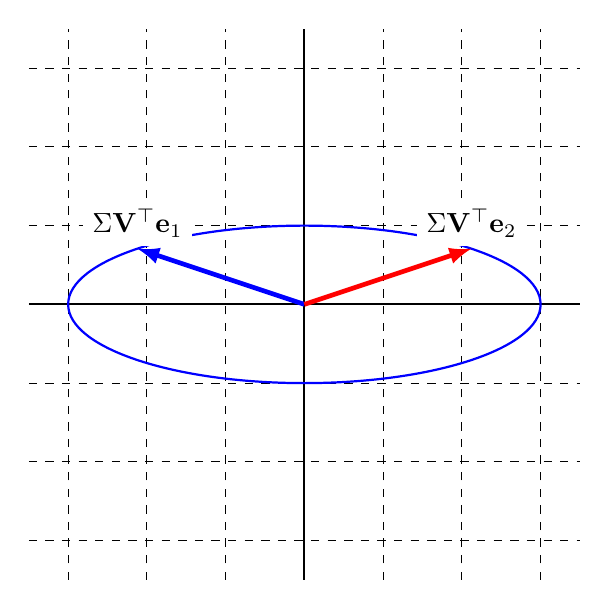
\begin{tikzpicture}
    \draw[thick] (-3.5,0) -- (3.5,0);
    \draw[thick] (0,-3.5) -- (0,3.5);
    \foreach \x in {-3,-2,-1,0,1,2,3}
      \draw[dashed] (\x,-3.5) -- (\x,3.5);
    \foreach \y in {-3,-2,-1,0,1,2,3}
      \draw[dashed] (-3.5,\y) -- (3.5,\y);

    \draw[color=blue, thick]  (0,0) ellipse (3 and 1);

    \draw[-latex,line width=0.6mm,color=blue]    (0,0) -- (-2.121, 0.707) node [above,color=black, fill=white]  {$\boldsymbol\Sigma \mathbf{V}^\top \mathbf{e}_1$};
    \draw[-latex,line width=0.6mm,color=red]     (0,0) -- ( 2.121, 0.707) node [above,color=black, fill=white]  {$\boldsymbol\Sigma \mathbf{V}^\top \mathbf{e}_2$};
  \end{tikzpicture}
  %\caption{$y=x$}
  %\label{fig:y equals x}
\end{subfigure}
\hfill
\begin{subfigure}[b]{0.45\textwidth}
  \centering
  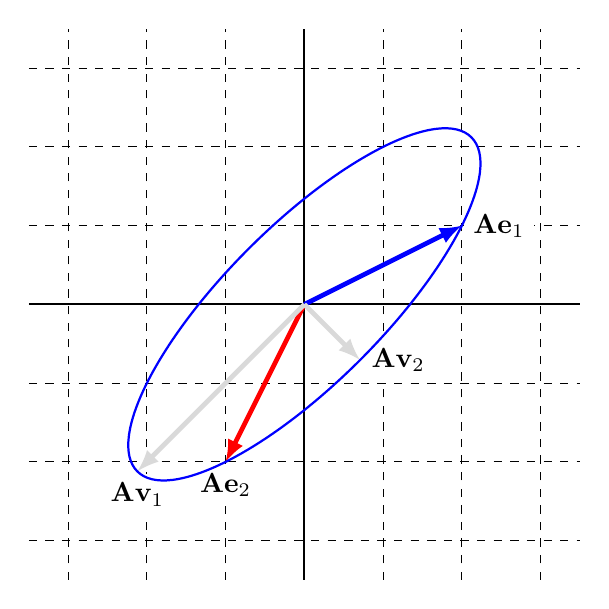
\begin{tikzpicture}
    \draw[thick] (-3.5,0) -- (3.5,0);
    \draw[thick] (0,-3.5) -- (0,3.5);
    \foreach \x in {-3,-2,-1,0,1,2,3}
      \draw[dashed] (\x,-3.5) -- (\x,3.5);
    \foreach \y in {-3,-2,-1,0,1,2,3}
      \draw[dashed] (-3.5,\y) -- (3.5,\y);



    \draw[-latex,line width=0.6mm,color=blue] (0,0) -- ( 2, 1) node [right,color=black,fill=white] {$\mathbf{A} \mathbf{e}_1$};
    \draw[-latex,line width=0.6mm,color=red] (0,0) -- (-1,-2) node  [below,color=black,fill=white] {$\mathbf{A} \mathbf{e}_2$};

    \draw[-latex,line width=0.6mm,color=gray!30] (0,0) -- (-2.121,-2.121) node [below,color=black,fill=white] {$\mathbf{A} \mathbf{v}_1$};
    \draw[-latex,line width=0.6mm,color=gray!30] (0,0) -- ( 0.707,-0.707) node [right,color=black,fill=white] {$\mathbf{A} \mathbf{v}_2$};

    \draw[color=blue, rotate=45, thick]  (0,0) ellipse (3 and 1);
  \end{tikzpicture}
  %\caption{$y=x$}
  %\label{fig:y equals x}
\end{subfigure}
\caption{Application of each operation from right to left of the singular value decomposition onto the unit basis vectors}
\label{Fig:linearAlgebra_illustrationSingularValueDecomposition}
\end{figure}

To illustrate the singular value decomposition, let us consider the action of $\mathbf{A} = \mathbf{U} \boldsymbol\Sigma \mathbf{V}^\top$ onto the unit basis vectors (i.e., the 2$\times$2 identity matrix), as depicted in Fig.~\ref{Fig:linearAlgebra_illustrationSingularValueDecomposition}. The top-left panel shows that the two unit basis vectors point along the $x$ and $y$ axes and lie on the unit circle. Note the description here applies to any unit vector, and the unit Cartesian basis vectors are chosen as an example.

Going from right to left, we first apply $\mathbf{V}^\top$ onto the unit basis vectors. Since $\mathbf{V}$ is unitary with all columns being unit vectors, the application of $\mathbf{V}$ or $\mathbf{V}^\top$ only reorients the vectors and does not stretch them. This reorientation is illustrated in the top-right panel of Fig.~\ref{Fig:linearAlgebra_illustrationSingularValueDecomposition}.

The application of $\boldsymbol\Sigma$ onto $\mathbf{V}^\top \mathbf{I}$ stretches the vectors along each principle coordinate direction by their respective singular value. In this case, the $x$ components are multiplied by a factor of $\sigma_1 = 3$ and the $y$ components are left as is because $\sigma_2 = 1$. This is shown in the lower-left panel of Fig.~\ref{Fig:linearAlgebra_illustrationSingularValueDecomposition}. The vectors after applying $\boldsymbol\Sigma$ now live on an ellipse rather than a circle.

Finally, the application of $\mathbf{U}$ onto $\boldsymbol\Sigma \mathbf{V}^\top \mathbf{I}$ completes the action of $\mathbf{A}$. This operation reorients the vectors, but does not change their magnitude because $\mathbf{U}$ is unitary, having columns that are orthonormal vectors. This also rotates the ellipse. This is drawn on the lower-right panel of Fig.~\ref{Fig:linearAlgebra_illustrationSingularValueDecomposition}; also depicted are the application of $\mathbf{A}$ onto the right singular vectors. The application of $\mathbf{A}$ onto any unit vector will yield another vector that points to some location on an ellipse. As can be seen in the figure, the application of $\mathbf{A}$ onto the right singular value $\mathbf{v}_1$, corresponding to the largest singular value $\sigma_1$, maps that vector onto the semi-major (or longest) axis of the ellipse, which is the maximum possible stretching. Note that the the application of $\mathbf{A}$ onto $\mathbf{v}_2$, which is the right singular vector corresponding to the smallest value, maps it onto the semi-minor axis, which is the smallest possible scaling.

The process for the singular value decomposition is as follows:
\begin{enumerate}
\item Given $N$$\times$$M$ matrix $\mathbf{A}$, compute $\mathbf{A}^\top \mathbf{A}$, which is an $M$$\times$$M$ real-symmetric matrix, and find its eigenvalues and eigenvectors. Since $\mathbf{A}^\top \mathbf{A}$ is real and symmetric, so we know its eigenvalues are real and nonnegative, there will be $r$ nonzero eigenvalues where $r$ is the rank of $\mathbf{A}$, and these $r$ eigenvectors should be orthogonal.
\item Sort the eigenvalues $\lambda_1 \ge \lambda_2 \ge \cdots \ge \lambda_r > 0$. Construct the matrix $\mathbf{V}$ by setting its columns equal to the eigenvectors of $\mathbf{A}^\top \mathbf{A}$ in the order of the eigenvalues.
\item Compute the singular values by taking the square root of the eigenvalues,
\begin{align}
  \sigma_i = \sqrt{\lambda_i} .
\end{align}
Construct the $N$$\times$$M$ matrix $\boldsymbol\Sigma$ by setting the diagonal elements $(i = j)$ to the singular values $\sigma_i$ in the same order as the eigenvectors. Note that a eigenvalue or singular value of zero occurs when the rank of the matrix $\mathbf{A}$ is smaller than~$N$.
\item Next, construct the first $r$ columns of the $N$$\times$$N$ matrix $\mathbf{U}$. This can be done by using the definition of the singular value decomposition given in Eq.~\eqref{Eqn:linearAlgebra_singularValueDecomposition}, noting that $\mathbf{V}$ is unitary and equal to its transpose (for real elements, or more generally its conjugate transpose), we can multiply the equation by $\mathbf{V}$ on the right to obtain
\begin{align} \label{Eqn:linearAlgebra_singularValueDecomposition}
  \mathbf{A V} = \mathbf{U} \boldsymbol\Sigma .
\end{align}
Since $\boldsymbol\Sigma$ is a diagonal matrix, we can write $\mathbf{U} \boldsymbol\Sigma$ as a matrix where each column is an (unknown) column of $\mathbf{U}$, call it $\mathbf{u}_i$, times the diagonal element $\sigma_i$ (a scalar singular value). Therefore, we can solve for each column as
\begin{align} \label{Eqn:singularValueDecomposition_computeUVectors}
  \mathbf{u}_i = \frac{1}{\sigma_i} \mathbf{A} \mathbf{v}_i .
\end{align}
\item If $r = N$, then we can go straight to the next step and form $\mathbf{U}$. Otherwise, if $r < N$, denoted by singular values $\sigma_i = 0$, then we need to find the remaining $N - r$ columns of $\mathbf{U}$. These columns must be orthonormal. These can be found using some orthogonalization procedure such as Gram-Schmidt process (see Sec.~\ref{Sec:linearAlgebra_CoordinateSystems_GramSchmidt}). To use this procedure, one needs to generate $N - r$ vectors that are linearly independent of all the other vectors in $\mathbf{U}$. Any linearly independent vector will do, so good candidates are often the unit basis vectors. Once these orthonormal vectors are computed, they should be inserted into the remaining columns of $\mathbf{U}$. Note that the $N - r$ orthonormal vectors are not unique, which implies the singular value decomposition is not unique when the rank of $\mathbf{A}$ is less than the number of rows~$N$.
\item Finally, we form $\mathbf{U}$ by using, from left to right, first the $r$ columns computed in step 4 in the same order as the singular values and then, if $r < N$, the remaining $N - r$ orthonormal vectors computed in step 5.
\end{enumerate}

Now we will do a few examples to illustrate this process.

%%%%%%%%%%%%%%%%%%%%%%%%%%%%%%%%%%%%%%%%%%%%%%%%%%%%%%%%%%%%%%%%%%%%%%%%%%%%%%%%%%%%%%%%%%%%%%%
\subsubsection{Example 1} 

Consider again the matrix we used earlier in this section:
\begin{align}
  \mathbf{A} = \left[ \begin{array}{c c}
   2 & -1 \\
   1 & -2 \\ \end{array} \right] .
\end{align}

Step 1 in the process involves computing $\mathbf{A}^\top \mathbf{A}$ and finding the eigenvalues and eigenvectors. First,
\begin{align}
  \mathbf{A}^\top \mathbf{A} = 
   \left[ \begin{array}{c c}
    2 &  1 \\
   -1 & -2 \\ \end{array} \right]
   \left[ \begin{array}{c c}
   2 & -1 \\
   1 & -2 \\ \end{array} \right] =
   \left[ \begin{array}{c c}
    5 & -4 \\
   -4 &  5 \\ \end{array} \right] .    
\end{align}
Observe that this a real symmetric matrix, which is guaranteed to have real and nonnegative eigenvalues. Compute the eigenvalues by evaluating
\begin{align}
   \left| \begin{array}{c c}
    5 - \lambda & -4 			\\
   -4 			&  5 - \lambda 	\\ \end{array} \right| = ( 5 - \lambda )^2 - 16 = \lambda^2 - 10 \lambda + 9 = 0, \quad \lambda = 9, 1.
\end{align}
Inserting each eigenvalue into the matrix $\mathbf{A}^\top \mathbf{A}$ and finding where it equals zero yields the eigenvectors. Doing this and applying elementary row operations gives
\begin{subequations}
\begin{align}
   &\lambda_1 = 9 : \quad 
   \left[ \begin{array}{c c}
   -4 & -4 	\\
   -4 & -4 	\\ \end{array} \right] \rightarrow
   \left[ \begin{array}{c c}
    1 &  1 	\\
    0 &  0 	\\ \end{array} \right] , \quad
    \mathbf{v}_1 = \frac{1}{\sqrt{2}} \left[ \begin{array}{c} -1 \\ 1 \\ \end{array} \right] ; \\
   &\lambda_2 = 1 : \quad 
   \left[ \begin{array}{c c}
    4 & -4 	\\
   -4 &  4 	\\ \end{array} \right] \rightarrow
   \left[ \begin{array}{c c}
    1 & -1 	\\
    0 &  0 	\\ \end{array} \right] , \quad
    \mathbf{v}_2 = \frac{1}{\sqrt{2}} \left[ \begin{array}{c} 1 \\ 1 \\ \end{array} \right] .
\end{align}
\end{subequations}
Note that the eigenvectors are normalized to be unit vectors and are orthogonal.

Step 2 involves forming the matrix $\mathbf{V}$ taking the eigenvectors and putting them as the columns in descending order of the magnitude of the eigenvalue:
\begin{align}
  \mathbf{V} = \frac{1}{\sqrt{2}}    \left[ \begin{array}{c c}
   -1 &  1 	\\
    1 &  1 	\\ \end{array} \right] .
\end{align}

Step 3 is to form the matrix $\boldsymbol\Sigma$ by taking the square root of the eigenvalues to compute the singular values and putting them along the diagonal and zeroes elsewhere:
\begin{align}
  \boldsymbol\Sigma = \left[ \begin{array}{c c}
   \sqrt{9} &  0 		\\
    0 		&  \sqrt{1} \\ \end{array} \right] = \left[ \begin{array}{c c}
    3	 	&  0 		\\
    0 		&  1		 \\ \end{array} \right] .
\end{align}

We observe that we have two nonzero singular values. Therefore, the rank of the matrix $\mathbf{A}$ is $r = 2$. Step 4 involves computing the first $r = 2$ columns of matrix $\mathbf{U}$ by Eq.~\eqref{Eqn:singularValueDecomposition_computeUVectors}. These are
\begin{subequations}
\begin{align}
  \mathbf{u}_1 &= \frac{1}{3} \frac{1}{\sqrt{2}} 
  \left[ \begin{array}{c c}
   2 & -1 \\
   1 & -2 \\ \end{array} \right] 
  \left[ \begin{array}{c} -1 \\ 1 \\ \end{array} \right] =
  \frac{1}{ \sqrt{2} } \left[ \begin{array}{c} -1 \\ -1 \\ \end{array} \right] , \\
  \mathbf{u}_2 &= \frac{1}{1} \frac{1}{\sqrt{2}} 
  \left[ \begin{array}{c c}
   2 & -1 \\
   1 & -2 \\ \end{array} \right] 
  \left[ \begin{array}{c} 1 \\ 1 \\ \end{array} \right] =
  \frac{1}{ \sqrt{2} } \left[ \begin{array}{c}  1 \\ -1 \\ \end{array} \right] .
\end{align}
\end{subequations}

Since the rank $r = 2$, which is equal to the number of rows (and columns) of the matrix, the matrix is said to be full rank. We therefore, have all the required orthonormal vectors to form $\mathbf{U}$ and can skip step 5 and proceed to step 6. Forming the matrix $\mathbf{U}$ with the vectors computing in step 4 gives the resulting matrix:
\begin{align}
  \mathbf{U} = \frac{1}{\sqrt{2}}    \left[ \begin{array}{c c}
   -1 &  1 	\\
   -1 & -1 	\\ \end{array} \right] .
\end{align}


%%%%%%%%%%%%%%%%%%%%%%%%%%%%%%%%%%%%%%%%%%%%%%%%%%%%%%%%%%%%%%%%%%%%%%%%%%%%%%%%%%%%%%%%%%%%%%%
\subsubsection{Example 2}

The previous example uses a full-rank matrix, so we could skip step 5 having an orthonormalization process. Let us now consider a case where the matrix is not full rank:
\begin{align}
  \mathbf{A} = \left[ \begin{array}{c c c c}
   1 &  0 & -1 &  0 \\
   0 &  1 &  0 &  1 \\
   1 &  1 & -1 &  1 \\
   1 & -1 & -1 & -1 \\ \end{array} \right] .
\end{align}
It is easy to observe that the third and fourth rows are, respectively, the sum and difference of the first and second rows.

Step 1 involves finding $\mathbf{A}^\top \mathbf{A}$ and computing the eigenvalues and the eigenvectors. First,
\begin{align}
  \mathbf{A}^\top \mathbf{A} = \left[ \begin{array}{c c c c}
   3 &  0 & -3 &  0 \\
   0 &  3 &  0 &  3 \\
  -3 &  0 &  3 &  0 \\
   0 &  3 &  0 &  3 \\ \end{array}  \right] .
\end{align}
Evaluate the determinant to find the eigenvalues:
\begin{align}
  \left| \begin{array}{c c c c}
   3 - \lambda &  0 & -3 &  0 \\
   0 &  3 - \lambda &  0 &  3 \\
  -3 &  0 &  3 - \lambda &  0 \\
   0 &  3 &  0 &  3 - \lambda \\ \end{array} \right| = \lambda^4 - 12 \lambda^3 + 36 \lambda^2 = \lambda^2 ( 6 - \lambda )^2 , \quad \lambda = 6, 6, 0, 0.
\end{align}
The eigenvectors, in the order of $\lambda_1 = 6, \lambda_2 = 6, \lambda_3 = 0, \lambda_4 = 0$ are
\begin{align}
  \mathbf{v}_1 = \frac{1}{\sqrt{2}} \left[ \begin{array}{c}  0 \\  1 \\  0 \\  1 \\ \end{array} \right] , 
  \mathbf{v}_2 = \frac{1}{\sqrt{2}} \left[ \begin{array}{c} -1 \\  0 \\  1 \\  0 \\ \end{array} \right] , 
  \mathbf{v}_3 = \frac{1}{\sqrt{2}} \left[ \begin{array}{c}  0 \\ -1 \\  0 \\  1 \\ \end{array} \right] , 
  \mathbf{v}_4 = \frac{1}{\sqrt{2}} \left[ \begin{array}{c}  1 \\  0 \\  1 \\  0 \\ \end{array} \right] .
\end{align}
Note that despite there being repeated eigenvalues, we still have four linearly independent eigenvectors.

In step 2, we construct the matrix $\mathbf{V}$ from the eigenvectors, which are already in the order of descending eigenvalue:
\begin{align}
  \mathbf{V} = \frac{1}{\sqrt{2}} \left[ \begin{array}{c c c c}
   0 & -1 &  0 &  1 \\
   1 &  0 &  1 &  0 \\
   0 &  1 &  0 &  1 \\
   1 &  0 &  1 &  0 \\ \end{array} \right] .
\end{align}
Note that one could swap the first and second columns or third and fourth columns, since they belong to a repeated eigenvalue.

Step 3 has us computing the matrix of singular values by taking the square root of the eigenvalues and placing them along the diagonal:
\begin{align}
  \boldsymbol\Sigma =  \left[ \begin{array}{c c c c}
   \sqrt{6} &  0 &  0 &  0 \\
   0 &  \sqrt{6} &  0 &  0 \\
   0 &  0 &  0 &  0 \\
   0 &  0 &  0 &  0 \\ \end{array} \right] .
\end{align}

Step 4 is computing the first $r$ columns of $\mathbf{U}$. Here $r = 2$, which corresponds to the number of nonzero singular values. We have
\begin{subequations}
\begin{align}
  \mathbf{u}_1 &= \frac{1}{\sqrt{6}} \frac{1}{\sqrt{2}} 
  \left[ \begin{array}{c c c c}
   1 &  0 & -1 &  0 \\
   0 &  1 &  0 &  1 \\
   1 &  1 & -1 &  1 \\
   1 & -1 & -1 & -1 \\ \end{array} \right] 
  \left[ \begin{array}{c}  0 \\  1 \\  0 \\  1 \\ \end{array} \right] =
  \frac{1}{ \sqrt{3} } \left[ \begin{array}{c} 0 \\  1  \\  1 \\ -1 \\ \end{array} \right] , \\
  \mathbf{u}_2 &= \frac{1}{\sqrt{6}} \frac{1}{\sqrt{2}} 
  \left[ \begin{array}{c c c c}
   1 &  0 & -1 &  0 \\
   0 &  1 &  0 &  1 \\
   1 &  1 & -1 &  1 \\
   1 & -1 & -1 & -1 \\ \end{array} \right] 
  \left[ \begin{array}{c} -1 \\  0 \\  1 \\  0 \\ \end{array} \right] =
  \frac{1}{ \sqrt{3} } \left[ \begin{array}{c} -1 \\  0  \\ -1 \\ -1 \\ \end{array} \right] .
\end{align}
\end{subequations}

Step 5 requires finding two additional orthonormal vectors with respect to $\mathbf{u}_1$ and $\mathbf{u}_2$. This may be done using the Gram-Schmidt orthogonalization procedure. To do this, we require any two additional vectors that are linearly independent with the others. Two acceptable choices are the unit basis vectors
\begin{align}
  \mathbf{w}_3 = \left[ \begin{array}{c} 1 \\  0  \\ 0 \\ 0 \\ \end{array} \right] , \quad
  \mathbf{w}_4 = \left[ \begin{array}{c} 0 \\  1  \\ 0 \\ 0 \\ \end{array} \right] .
\end{align}
It is easy to check that these cannot be written as a linear combination of each other or with $\mathbf{u}_1$ and $\mathbf{u}_2$. The unnormalized vector for $\mathbf{u}_3$ is obtained by taking
\begin{subequations}
\begin{align}
  \tilde{\mathbf{u}}_3 	= \mathbf{w}_3 
                   		- \left( \frac{ \mathbf{w}_3 \cdot \mathbf{u}_1 }{ \mathbf{u}_1 \cdot \mathbf{u}_1 } \right) \mathbf{u}_1
						- \left( \frac{ \mathbf{w}_3 \cdot \mathbf{u}_2 }{ \mathbf{u}_2 \cdot \mathbf{u}_2 } \right) \mathbf{u}_2 , \quad
  \mathbf{u}_3 =  \frac{1}{\sqrt{6}} \left[ \begin{array}{c} 2 \\  0  \\ -1 \\ -1 \\ \end{array} \right] .
\end{align}
Here $\tilde{\mathbf{u}}_3$ is the unnormalized version of $\mathbf{u}_3$. The actual vector $\mathbf{u}_3$ is computed by taking $\tilde{\mathbf{u}}_3/|\tilde{\mathbf{u}}_3|$. Finally, the vector $\mathbf{u}_4$ is computed by
\begin{align}
  \tilde{\mathbf{u}}_4 	&= \mathbf{w}_4 
                   		- \left( \frac{ \mathbf{w}_4 \cdot \mathbf{u}_1 }{ \mathbf{u}_1 \cdot \mathbf{u}_1 } \right) \mathbf{u}_1
						- \left( \frac{ \mathbf{w}_4 \cdot \mathbf{u}_2 }{ \mathbf{u}_2 \cdot \mathbf{u}_2 } \right) \mathbf{u}_2 
						- \left( \frac{ \mathbf{w}_4 \cdot \mathbf{u}_3 }{ \mathbf{u}_3 \cdot \mathbf{u}_3 } \right) \mathbf{u}_3, \nonumber \\
  \mathbf{u}_4 &=  \frac{1}{\sqrt{6}} \left[ \begin{array}{c} 0 \\  2  \\ -1 \\ 1 \\ \end{array} \right] .
\end{align}
\end{subequations}
It is important to note that the choices for $\mathbf{w}_3$ and $\mathbf{w}_4$ are arbitrary so long as they satisfy the criteria of being linearly independent with themselves and $\mathbf{u}_1$ and $\mathbf{u}_2$. This means that $\mathbf{u}_3$ and $\mathbf{u}_4$ are not unique, and there are infinitely many valid choices that could be used to form the matrix $\mathbf{U}$ and reproduce $\mathbf{A}$.

Step 6 forms the matrix $\mathbf{U}$ from the column vectors from steps 4 and 5:
\begin{align}
  \mathbf{U} = \frac{1}{\sqrt{6}} \left[ \begin{array}{c c c c}
   0 		& -\sqrt{2} &  2 &  0 \\
   \sqrt{2} &  0	 	&  0 &  2 \\
   \sqrt{2} & -\sqrt{2} & -1 & -1 \\
  -\sqrt{2} & -\sqrt{2} & -1 &  1 \\ \end{array} \right] .
\end{align}

%%%%%%%%%%%%%%%%%%%%%%%%%%%%%%%%%%%%%%%%%%%%%%%%%%%%%%%%%%%%%%%%%%%%%%%%%%%%%%%%%%%%%%%%%%%%%%%
\subsubsection{Example 3}

The previous two examples used square matrices. The singular value decomposition, however, is defined for any matrix. Let us compute this for a 2$\times$3 matrix:
\begin{align}
  \mathbf{A} = \left[ \begin{array}{c c c}
   2 &  0 & -1 \\
   1 &  1 &  0 \\ \end{array} \right] .
\end{align}

In step 1, we compute $\mathbf{A}^\top \mathbf{A}$,
\begin{align}
  \mathbf{A}^\top \mathbf{A} = 
  \left[ \begin{array}{c c}
   2 &  1 \\
   0 &  1 \\ 
  -1 &  0 \\ \end{array}  \right]
   \left[ \begin{array}{c c c}
   2 &  0 & -1 \\
   1 &  1 &  0 \\ \end{array}  \right] =
   \left[ \begin{array}{c c c}
   5 &  1 & -2 \\
   1 &  1 &  0 \\ 
  -2 &  0 &  1 \\ \end{array} \right] ,
\end{align}
and compute the eigenvalues,
\begin{subequations}
\begin{align}
  \lambda_1 = 6, \quad \lambda_2 = 1, \quad \lambda_3 = 0,
\end{align}
and the corresponding eigenvectors,
\begin{align}
  \mathbf{v}_1 = \frac{1}{\sqrt{30}} \left[ \begin{array}{c}  5 \\  1 \\ -2 \\ \end{array} \right], \quad 
  \mathbf{v}_2 = \frac{1}{\sqrt{ 5}} \left[ \begin{array}{c}  0 \\  2 \\  1 \\ \end{array} \right], \quad 
  \mathbf{v}_3 = \frac{1}{\sqrt{ 6}} \left[ \begin{array}{c}  1 \\ -1 \\  2 \\ \end{array} \right].
\end{align}
\end{subequations}
Note that there are two nonzero eigenvalues, signifying that $\mathbf{A}$ has a rank of 2. This is the maximum one could expect from a 2$\times$3 matrix.

Step 2 forms the matrix $\mathbf{V}$ from the eigenvectors. This is
\begin{align}
  \mathbf{V} = \frac{1}{\sqrt{30}} \left[ \begin{array}{c c c}
   5 &  0 			&   \sqrt{5} \\
   1 &  2\sqrt{6} 	&  -\sqrt{5} \\
  -2 &   \sqrt{6} 	&  2\sqrt{5} \\ \end{array} \right] .
\end{align}
Observe that the matrix $\mathbf{V}$ is a square matrix dimensioned by the number of columns of $\mathbf{A}$.

Step 3 computes the matrix $\boldsymbol\Sigma$ of singular values. This matrix is the same dimension as $\mathbf{A}$ or 2$\times$3. In this case, we populate the only two diagonal elements with the nonzero singular values, which are computed by taking the square root of the eigenvalues. This is then
\begin{align}
  \boldsymbol\Sigma = \left[ \begin{array}{c c c}
  \sqrt{6}	& 0		& 0		\\
  0			& 1		& 0		\\ \end{array} \right] .
\end{align}

In step 4, we compute the first $r = 2$ columns of the matrix $\mathbf{U}$. This is a square matrix with the dimension corresponding to the number of rows of $\mathbf{A}$, so 2$\times$2. Since the rank equals the number of columns of $\mathbf{U}$, we can determine all the left singular vectors $\mathbf{u}$ in this step. We have
\begin{subequations}
\begin{align}
  \mathbf{u}_1 &= \frac{1}{\sqrt{6}} \frac{1}{\sqrt{30}} 
   \left[ \begin{array}{c c c}
   5 &  1 & -2 \\
   1 &  1 &  0 \\ 
  -2 &  0 &  1 \\ \end{array} \right] 
  \left[ \begin{array}{c}  5 \\  1 \\ -2 \\ \end{array} \right] =
  \frac{1}{ \sqrt{5} } \left[ \begin{array}{c} 2 \\  1 \\ \end{array} \right] , \\
  \mathbf{u}_2 &= \frac{1}{\sqrt{5}} 
   \left[ \begin{array}{c c c}
   5 &  1 & -2 \\
   1 &  1 &  0 \\ 
  -2 &  0 &  1 \\ \end{array} \right] 
  \left[ \begin{array}{c}  0 \\  2 \\  1 \\ \end{array} \right] =
  \frac{1}{ \sqrt{5} } \left[ \begin{array}{c} -1 \\  2 \\ \end{array} \right] .
\end{align}
\end{subequations}

Since we have all the needed left singular values, we skip step 5 and move onto step 6 and form the $\mathbf{U}$ matrix from the vectors computed in step 4:
\begin{align}
  \mathbf{U} = \frac{1}{\sqrt{5}} \left[ \begin{array}{c c}
  2		& -1	\\
  1		&  2	\\ \end{array} \right] .
\end{align}

%%%%%%%%%%%%%%%%%%%%%%%%%%%%%%%%%%%%%%%%%%%%%%%%%%%%%%%%%%%%%%%%%%%%%%%%%%%%%%%%%%%%%%%%%%%%%%%
\subsection{Matrix Pseudoinverse}

A given matrix $\mathbf{A}$ only has an inverse if it is full rank, i.e., its rank is equal to the number of rows and columns. Just as the singular values exist for any matrix $\mathbf{A}$, there is a generalization of the inverse called the \emph{pseudoinverse} that exists for any matrix $\mathbf{A}$, which is denoted by $\mathbf{A}^+$. The singular value decomposition can always be used to compute $\mathbf{A}^+$.

The pseudoinverse is useful when finding optimal solutions given by linear systems that have incomplete information (such that there are infinitely many solutions) or are inconsistent (such that there are no unique solutions). This case often arises in practice because the amount of data we can collect is often far less than the number of model parameters, so we cannot uniquely determine the solution, but can only find one that best fits the data. Furthermore, when making experimental measurements, there is always some associated error or uncertainty, which means that the linear system could be inconsistent and, again, one has to settle for a solution that best matches the data. This notion is what connects the singular value decomposition, via the computation of the psuedoinverse, to optimization problems.

The pseudoinverse discussed here is sometimes called the Moore-Penrose inverse and is unique for a given matrix $\mathbf{A}$. There are four criteria that the psuedoinverse must satisfy
\begin{subequations}
\begin{align}
  &\mathbf{A} \mathbf{A}^+ \mathbf{A} = \mathbf{A}, \\*
  &\mathbf{A}^+ \mathbf{A} \mathbf{A}^+ = \mathbf{A}^+, \\*
  &\left( \mathbf{A} \mathbf{A}^+ \right)^* = \mathbf{A} \mathbf{A}^+ , \\*
  &\left( \mathbf{A}^+ \mathbf{A} \right)^* = \mathbf{A}^+ \mathbf{A} .  
\end{align}
\end{subequations}
Note that one could generalize an inverse to satisfy a subset of these four criteria, but then $\mathbf{A}^+$ would not be unique. Recall that the ``star'' superscript denotes the conjugate transpose, which, for real matrices is just the transpose. Another important property is that if $\mathbf{A}$ is full rank, then $\mathbf{A}^+ = \mathbf{A}^{-1}$. In a sense, the inverse is a special case of the pseudoinverse. One other fact about the pseudoinverse is that if $\mathbf{A}$ is $N$$\times$$M$ then $\mathbf{A}^+$ is $M$$\times$$N$.

There are special cases for which the pseudoinverse can be computed. One such important case is a rectangular $N$$\times$$M$ diagonal matrix $\mathbf{D}$, which has potentially nonzero values on the diagonal elements ($i = j$) and zeros everywhere else. (This is the case for the matrix $\boldsymbol\Sigma$ in the singular value decomposition). One can show (through) much effort, that the pseudoinverse of rectangular diagonal matrix is the transpose of that matrix with all of the nonzero diagonal elements inverted. For example:
\begin{align}
  \mathbf{D}_1 = \left[ \begin{array}{c c c}
  2		&  0	& 0		\\
  0		& -1	& 0		\\ \end{array} \right] , \quad 
 \mathbf{D}_1^+ = \left[ \begin{array}{c c}
  \frac{1}{2}	&  0	\\
  0				& -1	\\ 
  0				&  0	\\ \end{array} \right] ; \nonumber \\
  \mathbf{D}_2 = \left[ \begin{array}{c c}
  \frac{1}{3}	&  0			\\
  0				& \frac{2}{3}	\\ 
  0				& 0				\\
  0				& 0				\\ \end{array} \right] , \quad 
 \mathbf{D}_2^+ = \left[ \begin{array}{c c c c}
  3		&  0			&  0		&  0		\\
  0		&  \frac{3}{2}	&  0		&  0		\\ \end{array} \right] . \nonumber 
\end{align}
This can be shown by writing the general form for tall or wide rectangular diagonal matrices and showing that they satisfy the four criteria given above. (This is not done here because the derivation is rather tedious.)

The general method for computing a pseudoinverse uses the singular value decomposition and is given by
\begin{align}
  \mathbf{A}^+ = \mathbf{V} \boldsymbol\Sigma^+ \mathbf{U}^\top .
\end{align}
Since $\boldsymbol\Sigma$ is a rectangular diagonal matrix, it can be computed in the manner described previously.

To illustrate this, let us compute the pseudoinverse for the examples in Sec.~\ref{Sec:linearAlgebra_singularValueDecomposition}. The matrix for the first example is
\begin{align}
  \mathbf{A} = \left[ \begin{array}{c c}
   2 & -1 \\
   1 & -2 \\ \end{array} \right] . \nonumber
\end{align}
Using the previously obtained results, the pseudoinverse is then
\begin{align}
  \mathbf{A}^+ = 
  \frac{1}{2}    \left[ \begin{array}{c c}
   -1 &  1 	\\
    1 &  1 	\\ \end{array} \right] 
  \left[ \begin{array}{c c}
    \frac{1}{3}	 	&  0 		\\
    0 				&  1		\\ \end{array} \right] 
  \left[ \begin{array}{c c}
   -1 & -1 	\\
    1 & -1 	\\ \end{array} \right] = 
  \frac{1}{3} \left[ \begin{array}{c c}
    2	 	& -1 		\\
    1 		& -2		\\ \end{array} \right] .
\end{align}
Note that the pseudoinverse is identical to the actual inverse in this case since the matrix $\mathbf{A}$ is full rank.

In the second example, the matrix is
\begin{align}
  \mathbf{A} = \left[ \begin{array}{c c c c}
   1 &  0 & -1 &  0 \\
   0 &  1 &  0 &  1 \\
   1 &  1 & -1 &  1 \\
   1 & -1 & -1 & -1 \\ \end{array} \right] .
\end{align}
This matrix again is not full rank because the third and fourth rows are linear combinations of the first and second rows. The pseudoinverse is
\begin{align}
  \mathbf{A}^+ &= \frac{1}{\sqrt{2}} \frac{1}{\sqrt{6}}  \left[ \begin{array}{c c c c}
   0 & -1 &  0 &  1 \\
   1 &  0 &  1 &  0 \\
   0 &  1 &  0 &  1 \\
   1 &  0 &  1 &  0 \\ \end{array} \right] 
  \left[ \begin{array}{c c c c}
   \frac{1}{\sqrt{6}} &  0 &  0 &  0 \\
   0 &  \frac{1}{\sqrt{6}} &  0 &  0 \\
   0 &  0 &  0 &  0 \\
   0 &  0 &  0 &  0 \\ \end{array} \right]  
  \left[ \begin{array}{c c c c}
   0 		&  \sqrt{2} &  \sqrt{2} & -\sqrt{2} \\
  -\sqrt{2} &  0	 	& -\sqrt{2} & -\sqrt{2} \\
   2 		&  0 		& -1 		& -1 \\
   0 		&  2 		& -1 		&  1 \\ \end{array} \right] \nonumber \\
   &=
  \frac{1}{6} \left[ \begin{array}{c c c c}
   1 &  0 &  1 &  1 \\
   0 &  1 &  1 & -1 \\
  -1 &  1 & -1 & -1 \\
   0 &  1 &  1 & -1 \\ \end{array} \right] .
\end{align}

The matrix in the third example is
\begin{align}
  \mathbf{A} = \left[ \begin{array}{c c c}
   2 &  0 & -1 \\
   1 &  1 &  0 \\ \end{array} \right] . \nonumber
\end{align}
The pseudoinverse is
\begin{align}
  \mathbf{A}^+ &= 
  \frac{1}{\sqrt{30}} \frac{1}{\sqrt{5}}  \left[ \begin{array}{c c c}
   5 &  0 			&   \sqrt{5} \\
   1 &  2\sqrt{6} 	&  -\sqrt{5} \\
  -2 &   \sqrt{6} 	&  2\sqrt{5} \\ \end{array} \right] 
  \left[ \begin{array}{c c}
  \frac{1}{\sqrt{6}}	& 0		\\
  0						& 1		\\ 
  0						& 0		\\ \end{array} \right] 
  \left[ \begin{array}{c c}
  2		&  1	\\
 -1		&  2	\\ \end{array} \right] \nonumber \\
 &= \frac{1}{6} \left[ \begin{array}{c c}
   2 &  1 \\
  -2 &  5 \\ 
  -2 &  2 \\ \end{array} \right] .
\end{align}

%%%%%%%%%%%%%%%%%%%%%%%%%%%%%%%%%%%%%%%%%%%%%%%%%%%%%%%%%%%%%%%%%%%%%%%%%%%%%%%%%%%%%%%%%%%%%%%
\subsection{Example: Optimal Solution from Conflicting Data}

When taking measurements, for example, either in a controlled laboratory experiment or from sensor data of an industrial process, the data is never strictly consistent because of inherent uncertainties, random noise, and errors in collecting the data. A common task is to determine the ``best'' set of parameters that fits the measured data. There are many methods for doing this, and one approach applies the pseudoinverse. Suppose whatever process can be described by a system of linear equations with known coefficients (or at least those predicted from some model and taken as known) given in a matrix $\mathbf{A}$, measurement results given in a column vector $\mathbf{b}$, and a set of unknown parameters in solution vector $\mathbf{x}$. The matrix $\mathbf{A}$ need not be square and could simply contain multiple instances of the same equation or linear combinations thereof. 

In this case, there may be no inverse matrix and because of the contradictory information, there is no solution $\mathbf{x}$ that satisfies the system of linear equations $\mathbf{Ax} = \mathbf{b}$. Rather, we can find the ``best'' solution $\tilde{\mathbf{x}}$ from the equation
\begin{align}
  \mathbf{A}^+ \mathbf{b} = \tilde{\mathbf{x}}.
\end{align}
Here $\tilde{\mathbf{x}}$ is the best approximate for the solution vector $\mathbf{x}$ in that this choice minimizes
\begin{align}
  | \mathbf{b} - \mathbf{Ax} | , \nonumber
\end{align}
the magnitude of the difference between the measurements and $\mathbf{A}$ times the unknown model parameters $\mathbf{x}$.

For a numerical example, consider the mathematical model with three unknown variables and four measurements of different linear combinations of two of them
\begin{align}
  x + y &= 2, \nonumber \\
  y + z &= 1, \nonumber \\
  x - z &=  \frac{3}{2}, \nonumber \\
  x - z &=  \frac{3}{4}. \nonumber
\end{align}
Inspecting this system, the first two equations are independent. The third and fourth equations are identical except for the right-hand side being different (e.g. \, because of measurement uncertainties) and the left-hand side is the difference between the first and second equations. The matrix $\mathbf{A}$ for this system is
\begin{align}
  \mathbf{A} = \left[ \begin{array}{c c c}
   1 &  1 &  0 \\
   0 &  1 &  1 \\
   1 &  0 & -1 \\
   1 &  0 & -1 \\ \end{array} \right] .
\end{align}
Since this matrix is not square, we know that $\mathbf{A}^{-1}$ cannot exist. Furthermore, since the equations are obviously inconsistent, there is no solution vector that satisfies the linear system. While the inverse may not exist, the pseudoinverse does. This may be computed by taking the singular value decomposition and then computing the pseudoinverse from $\mathbf{A}^+ = \mathbf{V} \boldsymbol\Sigma^+ \mathbf{U}^\top$. The result of the singular value decomposition is
\begin{subequations}
\begin{align}
  \mathbf{V} &= \frac{1}{\sqrt{6}} \left[ \begin{array}{c c c}
  -\sqrt{3} 	&  1			&  \sqrt{2}			\\
   0			&  2			& -\sqrt{2}			\\
   \sqrt{3}		&  1			&  \sqrt{2}			\\ \end{array} \right] , \\
   \boldsymbol\Sigma &= \left[ \begin{array}{c c c}
   \sqrt{3}		&  0			&  0				\\
   0			&  \sqrt{5}		&  0				\\
   0			&  0			&  0				\\
   0			&  0			&  0				\\ \end{array} \right] , \\
  \mathbf{U} &= \frac{1}{\sqrt{30}} \left[ \begin{array}{c c c c} 
  -\sqrt{3}		&  \sqrt{15}	& -\sqrt{10}		& -\sqrt{2}				\\
   \sqrt{3}		&  \sqrt{15}	&  \sqrt{10}		&  \sqrt{2}				\\
  -2 \sqrt{3}	&  0			&  0				&  3 \sqrt{2}			\\
  -2 \sqrt{3}	&  0			&  \sqrt{10}		& -2 \sqrt{2}			\\ \end{array} \right] . 
\end{align}
\end{subequations} 
The pseudoinverse is then
\begin{align}
  \mathbf{A}^+ &= \frac{1}{15} \left[ \begin{array}{c c c c}
   4		&  1		&  3		& -3		\\
   5		&  5		&  0		&  0		\\
   1		&  4		& -3		& -3		\\ \end{array} \right] .
\end{align}
The solution vector that minimizes the difference between the measurement and $\mathbf{Ax}$ is
\begin{align}
  \tilde{\mathbf{x}} = 
  \frac{1}{15} \left[ \begin{array}{c c c c}
   4		&  1		&  3		& -3		\\
   5		&  5		&  0		&  0		\\
   1		&  4		& -3		& -3		\\ \end{array} \right]
   \left[ \begin{array}{c} 2 \\ 1 \\ \frac{3}{2} \\ \frac{3}{4} \\ \end{array} \right] =
   \left[ \begin{array}{c} \frac{3}{4} \\ 1 \\ -\frac{1}{20} \\ \end{array} \right] .
\end{align}
